\documentclass[a4paper,12pt]{article}
%\documentclass{aa}
\usepackage{conference}
\usepackage{latexsym}
\usepackage[perpage,symbol*]{footmisc}
%\usepackage[utf8]{inputenc}
\usepackage[utf8x]{inputenc}
\usepackage{textcomp}
\usepackage[french]{babel}
\usepackage{amssymb,amsfonts,amsmath} % blackboard math symbols
\usepackage{graphicx}                 % graphics
\usepackage{cite}
\usepackage[varg]{txfonts}
\usepackage{booktabs}                 % professional-quality tables
\usepackage{tabularx}
\usepackage{enumerate}
%\usepackage{enumitem}
\usepackage{multicol}
%\usepackage[utf8]{inputenc}          % allow utf-8 input
\usepackage[T1]{fontenc}              % use 8-bit T1 fonts
\usepackage{hyperref}                 % hyperlinks
\usepackage{url}                      % simple URL typesetting
\usepackage{nicefrac}                 % compact symbols for 1/2, etc.
\usepackage{microtype}                % microtypography
%\usepackage[final]{graphicx}
\usepackage{tocloft}
\usepackage{float}


%\marginsize{.5in}{.5in}{.75in}{.75in}
\cftsetindents{section}{0em}{2em}
\cftsetindents{subsection}{0em}{2em}
\renewcommand\cfttoctitlefont{\hfill\Large\bfseries}
\renewcommand\cftaftertoctitle{\hfill\mbox{}}
\setcounter{tocdepth}{3}

%\newcommand*{\grabto}[2]{\IfFileExists{#2}{}{\immediate\write18{curl \detokenize{#1 -o #2}}}}
%\grabto{https://www.pnas.org/content/pnas/15/3/168/F2.large.jpg}{hubble-orig.jpg}
%\begin{document}

\title{Retour au Cosmos}
\author{
  F.M. Sanchez~hol137\thanks{Professeur en retraite} \\
  Departement de physique\\
  Université Paris 11 Orsay \\
  Paris, FRANCE \\
  \texttt{hol137-at-yahoo.fr} \\
  %% examples of more authors
   \And
 M.H. Grosmann\thanks{Professeur en retraite} \\
  Departement de photonique\\
  Université de Strasbourg\\
  Strasbourg, FRANCE \\
  \texttt{michelgrosmann-at-me.com} \\
   \And
 D. Tassot\thanks{Ancien éleve de l'école des mines} \\
  Ecole des Mines\\
  %University of Strasbourg\\
  %Strasbourg, FRANCE \\
  \texttt{d.tassot-at-wanadoo.fr} \\
 %%  \And
 %% C. Bizouard\thanks{Astronome} \\
  % Observatoire de Paris\\
  % Paris, FRANCE \\
  %
 % \texttt{c.bizouard-at-obspm.fr} \\
  %% Coauthor \\
  %% Affiliation \\
  %% Address \\
  %% \texttt{email} \\
  %% \And
  %% Coauthor \\
  %% Affiliation \\
  %% Address \\
  %% \texttt{email} \\
  %% \And
  %% Coauthor \\
  %% Affiliation \\
  %% Address \\
  %% \texttt{email} \\
}


\begin{document}
\maketitle

%\{tableofcontents}
\tableofcontents
% \clearpage
% keywords can be removed
\keywords{Quantum \and Holography \and Cosmos}

\section*{Introduction}
\addcontentsline{toc}{section}{Introduction}

%\section{Introduction}

Le modèle dit du Big-Bang est une description de l'origine et de l'évolution de l’Univers datant du début du 20éme siècle.

De façon générale, le terme « Big Bang » est associé à toutes les théories qui décrivent notre Univers comme issu d'une dilatation rapide. Par extension, il est également associé à cette époque dense et chaude qu’aurait connue l’Univers il y a 13,8 milliards d’années, (sans que cela préjuge forcément de l’existence d’un « instant initial » ou d’un commencement à son histoire).

\subsection{Les deux modèles cosmologiques, le transitoire et le permanent}
\label{sec:headings}

Un modèle d'atome primordial a été initialement proposé en 1927 par l'astrophysicien  et chanoine catholique belge Georges Lemaître, qui décrivait dans les grandes lignes l’expansion de l'Univers, confirmée ensuite par les observations de l'astronome américain Edwin Hubble en 1929. Ce modèle fut désigné pour la première fois sous le terme ironique de « Big Bang » lors d’une émission de la BBC, The Nature of Things en 1949 (dont le texte fut publié en 1950), par le physicien britannique Fred Hoyle. C'était un terme qui se voulait moqueur, soulignant l'énormité d'une telle affirmation. Lui-même préférait les modèles d'état stationnaire, dans lequel la récession galactique est compensée par l'apparition spontanée de neutrons. Ceux-ci, se désintègrant après 880 secondes en proton, électron et neutrino, sont donc les "remontoires" de l'Univers, évitant ainsi la mort lente de l'Univers que nous promet le modèle trastoire des officiels.


Albert Einstein, en mettant au point la relativité générale, aurait pu déduire l'expansion de l'Univers, mais a préféré modifier ses équations en y ajoutant sa constante cosmologique, car il était persuadé que l'Univers devait être statique.


Il ne faut pas confondre ce modèle statique, d'ailleurs réfuté du fait de son instabilité foncière, avec le mdèle stationnaire de Hoyle dans lequel la récession galactique est justifiée, non pas par un Bang primordial, mais par la nécessité d'évacuer les galaxies, dont les soleils finiront par s'éteindre, pour faire de la place à de nouvelles galaxies. Ce modèle avait prévu l'accélération de la récession galactique, ce qui fut une totale surprise pour les officiels, qui ont cru, là encore, pouvoir s'en tirer en ajoutant un nouvel "épicycle", l'action d'une énergie noire répulsive. 


Pourquoi les officiels ont-ils choisi le modèle le plus compliqué, ajoutant les épicycles pour le sauver, comme au temps de Ptolémée. C'est que parmi ces 2 modèles un seul vraiment est réfutable, c'est-à-dire qu'on ne peut lui accoler d'épicyle, c'est le midèle permanent. Alors beaucoup se sont ingéniés à le réfuter. Une sociologie scentifique aberrante, détaillée dans le chapitre 6, a soutenu toute observation réfutant la permanece, et censuré toute observation la confirmant. C'est ainsi que les bébé-galaxies observées par Halton Arp ont été assimilées à des artéfacts.  

%Voir Section \ref{sec:headings}.

\subsubsection{La question du Cosmos}
%\lipsum[5]
Le concept général du Big Bang, à savoir que l’Univers est en expansion et a été plus dense et plus chaud par le passé, doit sans doute être attribué au Russe Alexandre Friedmann, qui l'avait proposé en 1922, cinq ans avant Lemaître. Son assise fut cependant considérée comme mieux établie en 1965 avec la découverte du fond diffus cosmologique. Georges Lemaître le qualifia d’« éclat disparu de la formation des mondes, attestant de façon définitive la réalité de l’époque dense et chaude de l’Univers primordial ». 

Mais il y a une interprétation beaucoup plus simple : c'est que notre Univers visible, tout immense qu'il soit, est immergé dans un Cosmos encore plus énorme qui lui envoie ce rayonnement. Le fait que ce soit un équilibre thermique quasi-parfait, avec une précision inégalée dans les laboratoires, milite en faveur de cette interprétation, car un Cosmos est forcément en équilibre thermique. 


On retrouve alors cete idée d'un Cosmos ordonné qui a traversé les âges (chapitre 1), mais qui a été oublié par nos contemporains, qui selon le mot du philosophe des sciences Jacques Merleau-Ponty, font de la "cosmologie sans Cosmos". C'est pourquoi cette solution beaucoup plus simple n'a même pas été considérée. Pour justifier la remarquable isotropie de ce rayonnement de fond, on a introduit un Big-Bang a 2 étapes, dans lequel une inflation qui gonfle l'Univer à une vitesse supra-luminique homgénéise ainsi l'espace. Ce grotesque "épicycle" est maintenant dénoncé par certains de ses partisans, car il pose plus de problèmes qu'il n'en résoud.


On a accepté cette inflation car elle explique une autre caractéristique révélée par le fond de rayonnement: le fait que la densité moyenne soit critique, c'est-à-dire celle d'un trou-noir. Or nous avons montré que la simple application du Principe Holographique implique cette condition critique. Les officiels n'ont pu appliquer ce principe à l'Univers, car ils considèrent son rayon d'horizon comme variable.

\subsubsection{la question de l'anti-matière}
   Selon le modèle standard le Big Bang aurait dû doner naissance à autant de matière que d'anti-matière. Or cette anti-matière ne se manifeste nulle part dans l'Univers. C'est ainsi que le cosmologue Jean-Pierre Petit a titré justement un ouvrange 'On a perdu la moitié de l'Univers". Le modèle standard des particules a été appelé à la escousse pour déceler une lègère dissymétrie entre particules et anti-particules pour justifier de l'anéantissement de ces dernières, mais sans succès.
   
   
    Certains ont introduits des univers parallèles évacuant l'anti-matière. Mais le plus simple est de rétablir la symétrie matière-anti-matière par la vibration très haute fréquence matière-antimatière (chapitre 3), une évidence logique qui a échappé aux pères fondateurs. 
    
    
    À noter l'intuition fulgurante de Matthieu Ricard dans son ouvrage écrit en commun avec l'astrophysicien Trinh Xuan Thuan\footnote{page 83, L'infini dans la paume de la main. Du big bang a l'éveil, avec Matthieu Ricard, Ed: Nil/Fayard, 2000}: ``Tant que toutes les causes et les conditions sont présentes, l'effet doit nécessairement être produit. S'il ne se produisait pas, cela voudrait dire qu'il manque encore quelque chose. Donc, si un principe créateur portait en lui toutes les causes et condition de l'univers, il devrait sans cesse créer la totalité de l'univers, un Big bang permanent en quelque sorte''. 
    
    
    En outre cet auteur note dans ses conclusions (page 419) : ``Pour le bouddhisme, quand on envisage la question d'un début, la seule position métaphysique qui résiste à l'analyse est celle de l'absence de début''.
    
   
   
 \subsubsection{la question du Multivers} 
Ultime épicycle: devant l'impossibilité d'expliquer les relations entre les paramètres physiques qui paraissent si favorables à la vie, certains cosmologues ont introduit l'idée du Multivers, provoquant un schisme sévère dans la communauté scentifique. Cette idée est réfutée ici par le rétablissement d'un Cosmos unique, parfaitement défini (chapitre 8) et l'identification des constantes biologiques et physiques (chapite 7).
 
 
  \subsubsection{la directive de Platon}

A la fin de ses Lois (ch 12, 961d) Platon déclare " pout éviter d'errer, les individus et les entités poltiques doivent se fixer un but unique et trouver le chemin singuier (statégie) qui conduit vers ce but.

Ce but unique est évidemment la compréhension du Cosmos. Le moyen qui conduit vers cette connaissance supr\^eme est la méthode scientifique de Pythagore : \textit {chercher les plus belles relations entre nombres entiers.}

Comme disait Hermès Trismégiste "ce qui est en bas est comme ce qui est en haut". L'homme peut appréhender l'énormité du Cosmos, car celui-ci l'a conçu pour l'accompagner dans sa qu\^ete de la plus belle relation entre les nombres entiers les plus petits et les plus grands.

      
    

\subsubsection{Retour au Cosmos}
Le chapitre 1 est donc consacré à l'historique de ce concept oublié, le Cosmos. L'idée de simplicité, si contraire aux préjugés officiels, conduit à réintroduire l'importance du concept de nombre entier, introduit par Pythagore (chapitre 2). Nous montrons ensuite (chapitre 3) comment des raisonnements très simples, basés sur l'holographie, conduisent à justifier l'énormité de l'Univers obervables, le modèle du Big Bang Permanent et préciser ses caractéristiques. Le chapitre 4 taite de la question si importante et si négligée des grands nombres. Le chapitre 5 rappelle l'état déplorable de la cosmologue standard, basée sur une sociologie aberrante, décrite chapitre 6. Le chapitre suivant explique comment on en est arrivé à perde quelques 30 ans en biologie médicale.

Le chapitre 8 précise la grande réunification philosophie-physique-arithmétique-biologie, la définition précise du Cosmos, ce qui conduit au chapitre 9 final sur les prospectives et prédictions.


\section{Le concept de Cosmos à travers les ages}

Brèves considérations historiques sur la notion de cosmos

On a souvent opposé les paysages de la Grèce, avec leur horizon toujours net et bien défini, et les paysages nordiques, souvent brumeux, où la ligne d'horizon échappe à l'observateur. Des premiers émerge l'idée qu'une perfection peut se réaliser dans la finitude, dans la statuaire par exemple ; des seconds l'attrait pour l'infini. 

Il n'est alors pas surprenant que l'Europe du Nord ait été le lieu de la grande révolution intellectuelle qui, au XVIIe siècle, fit passer « du monde clos à l'univers infini », pour reprendre le titre d'un ouvrage d'Alexandre Koyré. Ce dernier ramène le changement ainsi opéré « à deux éléments principaux, d'ailleurs étroitement liés entre eux, à savoir la destruction du cosmos et la géométrisation de l'espace, c'est-à-dire:

\textbf{a}) la destruction du monde conçu comme un tout fini et  \textbf{bien ordonné}, dans lequel la structure spatiale incarnait une hiérarchie de valeur et de perfection, monde dans lequel “au-dessus” de la terre lourde et opaque, centre de la région sublunaire, du changement et de la corruption, s'“élevaient” les sphères célestes des astres impondérables, incorruptible et lumineux, et la substitution à celui-ci d'un univers indéfini, et même infini, ne comportant plus aucune hiérarchie naturelle et uni seulement par l'identité des lois qui le régissent dans toutes ses parties, ainsi que par celle de ses composants ultimes placés, tous, au même niveau ontologique, et 

\textbf{b}) le remplacement de la conception aristotélicienne de l'espace, ensemble différencié de lieux intramondains, par celle de l'espace de la géométrie euclidienne – extension homogène et nécessairement infinie  – désormais considéré comme identique, en sa structure, avec l'espace réel de l'univers. Ce qui à son tour, implique le rejet par la pensée scientifique de toute considération basée sur les notions de valeur, de perfection, d'harmonie, de sens ou de fin, et finalement la dévalorisation complète de l’être, \textbf{le divorce total entre le monde des valeurs et le monde des faits} » \footnote{A. KOYRÉ, Du monde clos à l’univers infini (1957), trad. fr. Paris, Gallimard, 1973, p. 11-12.} [souligné par nous]

Sous ce langage un peu abstrait, l’historien des idées enseignant à Princeton, laissait entrevoir à quel point il s'agit d'une transformation profonde de la vision du monde, si profonde même qu'il nous est impossible, sans un effort de dépaysement, sans un minimum de sympathie pour les Anciens, de comprendre vraiment ce qu'ils ont dit et pensé. Les même êtres habitent leur monde et le nôtre, et leurs héros éprouvent les mêmes sentiments et les mêmes émotions que nous, mais leur terre, leur ciel et leur espace, bref leur habitacle, est tout autre.

Certes, la chrétienté avait modifié les relations entre les hommes \footnote{Il importe de ne pas idéaliser la société antique, comme l’ont fait les penseurs de la Renaissance. Admirer leur langage et leurs arts n’oblige pas à rester aveugles sur les multiples travers de ces civilisations polythéistes.} et transformé le culte divin, mais elle maintenait et même développait l'idée d'un « cosmos ». 
Le sens premier du mot, dans les dictionnaires du grec classique est « bon ordre », comme celui d'une armée qui défile. Il comporte une valeur, une appréciation. De quelque manière, le « et cela était bon » de Genèse 1 commandait la perception des êtres et des paysages. Il suffisait alors d'ouvrir les yeux pour découvrir un monde enchanté et vibrant où la beauté était omniprésente, y compris dans les objets usuels, les outils, les gestes \footnote{Ainsi « le geste auguste du semeur », inspirant à Victor Hugo son célèbre Saison des semailles. Le soir.} et les pensées. Le beau était d'ailleurs une des significations associée au mot « cosmos », celle qui s’est conservée dans « cosmétique » \footnote{Cosmetes ou cosmætria était l’esclave chargée de la toilette.}. 

On objectera que le « design » fait désormais partie de notre civilisation, que l'objet industriel a lui aussi sa beauté. Mais il s'agit d'une vertu surajoutée, d'un effort pour compenser ce qui n'était pas visé au départ, d’une forme de division du travail, d'une recomposition tardive de l'unité perdue au sein de l'acte producteur. C'est là une différence de nature entre l'objet artisanal où la visée esthétique peut être menée de front avec la fin utilitaire, et l’objet industriel dont la finalité première est l'utilité. De là encore cette note « humaine » qui transparaît dans les vieux objets et qui manque tant à notre environnement actuel. Dans « artisan » il y a « art ». Dans le dessin industriel, la beauté se présente encore, mais dans l’acte lui-même du dessinateur plus que dans le dessin réalisé ; ou alors c’est par ricochet, de par la beauté propre aux courbes géométriques.

Il semble que les pythagoriciens furent les premiers à donner à « cosmos » le sens de « monde », d'univers. Puis ce dernier mot s'est à ce point imposé que « cosmos » ne figure pas dans le Grand Larousse du XXe siècle. On y trouve bien cosmographie, cosmologie et cosmogonie, mais « cosmos » tout court y désigne une plante composée (le cosmos bipinnatus) et aussi le titre de la Description physique du globe d’Alexandre de Humboldt. 

Or il existe une nuance significative entre « cosmos » et « univers » \footnote{Le substantif « univers » apparaît au XVIe siècle.} : précisément celle qui différencie le monde des Anciens du nôtre. À l'époque où le charbon était encore un combustible courant, un bambin vint trouver sa mère qui bavardait au salon avec des amies. Il tenait à la main un morceau d'anthracite trouvé dans le jardin et dit : « Regarde, Maman, comme c’est beau ! » L'enfant vivait encore, à sa manière, dans le cosmos des anciens ; il suffira de quelques années sur les bancs de l'école pour qu'il apprenne que même un morceau d'anthracite, avec ses facettes brillantes, n'était qu'un corps très ordinaire, sans grande valeur marchande et, surtout, salissant.

Le « désenchantement du monde » \footnote{L’expression est attribuée au sociologue Max Weber.} était passé par là. Koyré – et il n'est pas le seul – fait commencer le processus au cardinal allemand Nicolas de Cues (1401-1464) « qui a inauguré le travail destructif qui mène à la démolition du cosmos bien ordonné, en mettant sur le même plan ontologique la réalité de la Terre et celle des Cieux. La Terre, nous dit-il, est une stella nobilis, une étoile noble, et c'est par là-même, autant que par l'affirmation de l'infinité ou plutôt de l'indétermination de l'univers, qu'il déclenche le processus de pensée qui aboutira à l'ontologie nouvelle, à la géométrisation de l'espace et à la disparition de la synthèse hiérarchique. \footnote{A. KOYRÉ, Etudes d’Histoire de la pensée scientifique, Paris, Gallimard, 1973, p. 54.} » 

Il convient donc, pour bien appréhender la « révolution » du XVIIe siècle, de revenir sur le cosmos des Anciens. On ne détruit bien que ce que l'on remplace, mais une dimension essentielle de l'antique vision du monde s'est perdue, nous allons le voir, en nous inspirant ici d'un essayiste et philosophe britannique, Philippe Scherrard \footnote{Ph. SHERRARD, Human Image : World Image. The death and resurrection of sacred cosmology, Limni, Evia, Grèce, Denise Harvey, 2004, (princeps par Golgonooza Press en 1992).}. Car les notions pourtant basiques d'espace, de temps, de cause et de mouvement n'ont plus aujourd'hui le sens plénier qui leur revenait dans le cosmos des anciens. Leur « physique », en effet, n'était pas une discipline autonome mais une partie d'un ensemble philosophique visant à appréhender les choses selon leur être profond, dont la quantité mesurable n'est qu'un aspect secondaire.

Alors l'homme, en tant que microcosme reflétant en lui-même tous les éléments de l'univers, tant immatériels que matériels, y trouvait sa place spécifique, aussi fondamentale qu’aujourd'hui la place du carbone ou de l'hydrogène. Ce composant non mesurable du cosmos y était même dominant, de par sa capacité à appréhender le monde archétypal des formes. 

Pour Platon la structure ou  \textbf{forme} qui est « dans » les choses naturelles ou dans les actes humains constitue leur essence. Celle-ci n'est pas la forme pure mais son imitation et, comme telle, aspire à la réalisation de la forme pure. Tout le monde de la nature est ainsi une copie de l'archétype des formes pures cherchant à atteindre la perfection et l'immortalité de ce modèle idéal. Ceci explique pourquoi notre monde est dans un perpétuel changement, mais avec une orientation objective finalisée. Et pourquoi la nature dépend-t-elle pour cette finalité de quelque chose qui la transcende ? Parce que – dit le Timée – « ce qui est engendré, c'est nécessairement par l'action d'une cause que cela est engendré. » \footnote{PLATON, Timée, 28c} Le monde de la nature est un monde de devenir et tout ce qui devient doit avoir une cause. Remarquons que par « cause » le grec ne se réfère pas, comme dans le langage moderne, purement à un évènement antérieur dans le temps à son effet ; il se réfère à tout ce qui donne une raison à l'existence, à l'apparence de quelque chose, sans référence temporelle nécessaire. 

Pour Aristote, le monde de la nature est animé d'un mouvement spontané. Mais ce changement n'est pas l'effet du hasard, il est dirigé vers une certaine fin. Comme pour Platon, les choses de la nature aspirent à réaliser certaines potentialités. Alors que dans le Timée, Dieu, le démiurge, façonne le monde selon le modèle des formes immatérielles archétypales du monde intelligible, chez Aristote Dieu, le seul moteur immobile, est identifié à ces formes qui constituent une sorte de pluralité d'intelligences formant un modèle immatériel et éternel. Pour Aristote comme pour Platon, la différentiation des choses dans la nature, de même que le processus de leur changement, dépendent logiquement (et même ontologiquement) mais non temporellement de la différentiation de leurs archétypes dans la réalité éternelle. C'est parce que ces archétypes représentent autant de modes intelligibles par lesquels Dieu manifeste sa propre activité, sa propre connaissance de Lui-même, qu'ils inspirent à toute la nature un désir ou un amour (eros) de Dieu, une aspiration vers Lui, chaque chose accomplissant cette aspiration dans la mesure où elle agit conformément à sa nature et à son rang et capacité. Tout ceci ne suppose aucune théorie de l'évolution au sens moderne. Le mouvement par lequel chaque chose croît et se développe afin de réaliser la loi de sa nature, n'est pas une évolution ; au contraire, il représente le processus de tension qui se produit entre chaque chose et son éternel archétype. 

Dans cette conception large du mouvement comme une transformation, comme le passage de la puissance à l’acte, le changement de lieu, le « mouvement local », n'était qu'un cas très particulier, inessentiel même, du mouvement. C'est pourquoi la physique aristotélicienne ne s'y est pas attardée, ce qui entraîna sa perte. Pour les Anciens, le repos est la fin naturelle visée par les choses, le point d'équilibre où elles réalisent leur nature. Le « bas » est ainsi le lieu naturel des corps « graves » \footnote{C’est l’étymologie du mot « gravitation ».} (les corps pesants), là où ils se tiennent en repos. Leur « mouvement local » naturel les fait donc tomber vers le centre de la Terre : ils réalisent ainsi leur nature, comme la flamme le fait en s’élevant vers le ciel. Dans cette perspective,  \textbf{tout mouvement (même non accéléré) requiert une cause agissante}, ainsi la tension de la corde qui propulse la flèche. Or, une fois lancée, la flèche poursuit son mouvement, et ce fut un point d'achoppement pour l'ancienne physique. On imagina, par exemple, que de petites fibres dans l'air propulsaient la flèche, entretenant ainsi le mouvement « violent » (appelé « violent » car entraînant la flèche hors de sa place propre dans l'univers, lui faisant donc violence). Aussi un tel mouvement doit-il s'arrêter un jour : rien de ce qui est contra naturam ne peut se perpétuer. Le « divin Archimède » lui-même ne sut élaborer que les principes d’une statique. 

Ce point, l'incapacité à bien expliquer la poursuite du mouvement des objets lancés, fut la chute de la physique aristotélicienne. On explique aujourd'hui ce mouvement par le principe d'inertie. On a ainsi érigé en postulat indémontré ce dont on ne sait toujours pas comprendre la cause. Le progrès a surtout consisté à montrer, et ce fut la gloire de Galilée, que le mouvement des corps obéit à des lois mathématiques, ce dont Aristote ne s'était jamais préoccupé puisque, pour lui, le mouvement « local » était secondaire, consistant en un simple déplacement sans nulle transformation au sens propre. Or la cause du mouvement, au sens véritable de « cause », n’est pas mieux atteinte parce qu'on a su quantifier ses différentes étapes, mesurant par exemple l'accélération de la chute des corps. 

La différence majeure a consisté ici plutôt en l'oubli des transformations qualitatives qui étaient l'objet principal des observations des Anciens. Il serait donc injuste de mépriser la science grecque et de la rejeter comme « dépassée ». La physique moderne a renoncé à expliquer la cause du mouvement ; elle ne prend en compte que l'accélération, la dérivée seconde. Alors, restée seule en scène, l'analyse mathématique devient reine et la découverte des lois du mouvement fut une avancée impérissable des fondateurs. Mais il y eut un prix à payer : la perte des qualités sensibles des corps, de leurs éléments qualitatifs. Ce fut la porte ouverte au grand « réductionnisme » encore à l'œuvre.

Les Kepler, Galilée, Descartes et Newton étaient de brillants mathématiciens, mais il leur manquait la sagesse. Par leur manque d'une plus profonde intelligence des choses, par leur ignorance de la vraie philosophie, ils identifièrent leur Dieu avec le grand mathématicien cosmique. Un système géométrique infini devint le véritable horizon métaphysique de la nature. Ceci veut dire que la structure de la nature est fondamentalement mathématique. Or une vision mathématique de la nature entraîne inévitablement une conception mécanique de ses opérations. Avec une telle vision, toutes les qualités non quantifiables du monde sont perdues, désacralisées, et les principes mathématiques en viennent à être des vérités supérieures à toutes les autres. 

Les pionniers de la science moderne instituèrent ainsi une nouvelle théorie de la nature, de ses changements et mouvements. Ceux-ci doivent être expliqués désormais par référence à l'action de choses matérielles déjà existantes. C'est l'action d'une ou plusieurs de ces choses matérielles qui engendre le mouvement d'autres choses, produisant ainsi les diverses structures de la nature. Selon cette vue, le changement n'est plus l'expression d'une aspiration vers un état transcendant et immortel de l'être ; il est simplement une fonction de la structure mathématique. À l'étude du pourquoi du mouvement est substituée l'étude du comment, et cette analyse est confiée aux mathématiques. Mais l'analyse mathématique du comment du mouvement implique inévitablement de considérer l'espace comme quelque chose de purement géométrique et le temps comme essentiellement mathématique. 

Traiter le mouvement mathématiquement revient à l'analyser en certaines unités de distance parcourues en certaines unités de temps. Mais alors, ceci veut dire que l'espace et le temps sont considérés comme des catégories objectives fondamentales, et que le monde réel est un monde de corps matériels se mouvant dans l'espace et le temps, le monde de la physique, considéré comme autonome et autosuffisant. Cette interprétation signifie que le temps et l'espace acquièrent un nouveau statut. Cela veut dire qu'on leur donne une nouvelle signification de continua mathématiques et qu'on les élève au rang de principes métaphysiques ultimes, indépendamment des corps matériels qui les occupent. Cette idée que la temporalité du mouvement est réductible en termes mathématiques signifie que le temps devient une irréversible quatrième dimension. Il est absolu, infini, homogène, continu, indépendant de tout objet sensible, coulant sans interruption d'éternité en éternité.

Sur ces points eut lieu un grand débat entre Leibniz et Newton. Selon la formulation du principe d’inertie par Newton, un corps demeure dans son état de mouvement rectiligne uniforme ou de repos, indépendamment de ce qui arrive aux autres corps, et demeurerait dans cet état de mouvement ou de repos, même s’il n’existait aucun autre corps. Mais alors, objecte Leibniz, « un tel mouvement ne produirait aucun changement observable, et  \textbf{serait sans but}. On \footnote{Ce « on » est ici le Dr Clarke qui prête sa plume à Newton dans cette correspondance avec Leibniz.} réplique maintenant que la vérité du mouvement est indépendante de l’observation ; et qu’un vaisseau peut avancer sans que celui qui est dedans s’en aperçoive.  \textbf{Je réponds que le mouvement est indépendant de l’observation ; mais qu’il n’est point indépendant de l’observabilité}. Il n’y a point de mouvement, quand il n’y a pas de changement du tout. Le contraire serait fondé sur la supposition d’une Espace réel absolu, que j’ai réfuté démonstrativement par le principe du besoin d’une raison suffisante des choses » \footnote{Correspondance Leibniz-Clarke présentée d’après les manuscrits originaux des bibliothèques de Hanovre et de Londres par André Robinet, Paris, P.U.F. 1957, n°52, p. 149.} [souligné par nous]

Se fait jour ici l'opposition entre un Leibniz philosophe, qui s'attache à sauver ce qui peut l'être de la métaphysique, qui fait du principe de raison suffisante une catégorie supérieure aux démonstrations quantitatives, et un Newton physicien qui n'hésite pas à faire de son espace un absolu. Or c’est Leibniz qui, avec la « force vive » ($mv^2$), a le mieux établi les fondements de la dynamique, réfutant l'erreur de Descartes qui croyait que la quantité de mouvement (mv) se conservait. On peut même dire que Leibniz fera de la statique un simple cas particulier de la dynamique : lorsque la vitesse tend vers l'infiniment petit. Pourtant, à la différence de Descartes ou de Newton, Leibniz, avec sa notion d’une « harmonie préétablie » s'efforçait de préserver la conception d'un cosmos cohérent. Ce mouvement perpétuel qu'on savait depuis les Grecs ne pas exister, il le voit régner à l'échelon global de la nature. 

Reste que la physique moderne a suivi les traces de Newton, fût-ce pour le dépasser. La compréhension du temps comme quelque chose dans laquelle nous  \textbf{vivons} réellement a disparu. Car si le temps est un  \textit{continuum} mesurable, il n'est rien de plus qu'une limite mathématique mouvante entre le passé et le futur. Il n'a plus d'actualité (au sens philosophique du terme) et même le moment présent ne possède plus de qualité temporelle : il est uniquement la limite éphémère dans un processus venant du passé et allant vers le futur avec indifférence et monotonie. Ensuite, cette conception du temps signifie que les humains en sont effectivement exclus. Car la notion de temps comme continuum mathématique oblige à penser la causalité seulement en termes de forces se révélant dans les mouvements de la matière exprimables mathématiquement. En fait, causes et effets sont maintenant vus comme des mouvements ; alors il n'y a plus qu'à affirmer que le monde est une vaste machine mathématique indépendante, consistant en mouvements de matière dans l'espace et le temps. Mais dans un monde vu comme une parfaite machine, il demeure peu ou pas de place pour l'homme.

Dans ce monde, l'homme est un hasard, un sous-produit passager et finalement superflu. Telle est la vision du monde, sûrement l'une des plus obscurantistes et inhumaines jamais sortie de l'esprit humain, qui est devenue la vision prédominante des temps modernes. Or la nature réelle, dans toute sa complexité, est aussi fondamentalement qualitative, composée de choses qui sont définies par leur finalité. Les catégories courantes par lesquels ces choses sont comprises et interprétées ne sont donc pas celles de temps, espace, masse, énergie, etc., mais bien celles de substance, essence, matière, forme, couleur, son, beauté, parfum, réceptivité à l'amour, à la joie, à la compassion, toutes qualités qui sont immédiatement présentes et pleinement intelligibles par nous dans les choses elles-mêmes. Lorsque l’on célèbre les fondateurs de la physique moderne, il ne faut donc pas oublier ce qu’ils ont laissé de côté dans leur marche triomphale pour mettre le monde en équations. Il y a une chose étrange dans Le Monde de Descartes. 

Il commence par présenter « son » Monde comme un monde imaginaire dans lequel opèrent de purs êtres mathématiques. Il s'épargne ainsi les critiques des philosophes aristotéliciens qui s'opposeraient à cette réduction des êtres à leurs dimensions quantitatives. C'est donc, avant la lettre, un « modèle » ne prétendant pas décrire la complexe réalité des choses. Puis, au fil des pages, on voit bien qu'il s'agit pour lui du monde réel qu’il se réjouit d'avoir traduit en lois et en propriétés mathématiques. De la même façon, l'espace newtonien s'identifie à un espace géométrique étendant à l'infini ses trois repères orthogonaux, espace dont la réalité ne doit rien aux corps matériels qui pourront éventuellement s’y trouver.

Aujourd'hui, trois siècles ont passé. Les innombrables applications de la science contemporaine semblent donner raison à Descartes : le monde réel serait donc bien tel qu'il l'avait imaginé « écrit en langage mathématique \footnote{« La filosofia è scritta in questo grandissimo libro, che continuamente ci sta aperto innanzi a gli occhi (io dico l’universo), ma non si può intendere se prima non s’impara a intender la lingua, e conoscer i caratteri, ne quali è scritto. Egli è scritto in lingua matematica, e i caratteri son triangoli, cerchi, ed altre figure geometriche, senza i quali mezi è impossibile a intenderne umanamente parola. ». GALILÉE, Il Saggiatore, in Le Opere di Galileo Galilei, Ed ; Nazionale, A. Favaro, Florence, 21 vol., 1890-1909, vol. VI, p. 232.} » (selon le mot de Galilée). Mais le prix à payer fut l'exclusion de cet univers de l'homme lui-même, devenu une sorte de spectateur étranger à l'habitacle qui est pourtant le sien. L'antique cosmos hiérarchisé, où la hiérarchie des êtres établit leur qualité, a pu sembler disparu à jamais. Reste cependant à savoir si le retour du cosmos, auquel nous assistons dans tous les domaines de la science, saura ressusciter les dimensions oubliées de l'ancien cosmos.






\subsection {La \textit{cosmologie sans le Cosmos} du philosophe Merleau-Ponty}

Extrait de Jean Seidengart et Jean-Jacques Szczeciniarz (éds.), Cosmologie et philosophie, en hommage à
Jacques Merleau-Ponty, Epistémologiques (Philosophie, sciences, histoire), vol. 1, n°1-2, 2000.



Et il constate
que les théoriciens de la physique, qui « malgré leurs traditionnelles dénégations
n'ont jamais cessé d'être philosophes », le sont redevenus au XXe siècle, « mais
c'est au sens réflexif et critique du mot “philosophie”, non au sens dogmatique de
la philosophie (soi-disant) perennis ». La méthode qu'il suit dans cet examen est
celle de l'épistémologie historique, qui ne s'interdit pas un regard récurrent tout en
respectant l'historicité. « Sans négliger l'histoire », écrit-il à ce sujet, « notre
méthode n'admet pas la règle stricte de ne pas chercher à comprendre un certain
présent par son avenir et c'est en fonction de ce que nous savons maintenant avoir
été leur avenir » qu'il a choisi les auteurs et les textes étudiés dans son ouvrage
(Galilée, Ampère, et Einstein).


Son livre La science de l'Univers à l'âge du positivisme, sous-titré
Etude sur les origines de la cosmologie contemporaine, paru en 1983, tout en étant
un livre d'histoire des sciences au sens propre, profite de l'éclairage que permet le
« devenir » des conceptions étudiées, réalisé tant dans la physique que dans la
cosmologie contemporaines. D'ailleurs, le problème examiné lui-même n'aurait pu
être formulé sans cet éclairage. Mais une fois qu'il est ainsi éclairé, c'est à une
analyse des oeuvres telles qu'on peut les connaître selon les textes et la pensée de
leurs auteurs que s'attache l'épistémologue-historien. Ces auteurs sont tout d'abord
« deux des plus grands cosmologues de tous les temps », Pierre-Simon Laplace et
William Herschel, qui travaillèrent indépendamment, tous deux à la charnière du
XVIIIe et du XIXe siècles, et sur des registres bien différents : Laplace en astronomie
mathématique, avec son Système du Monde et son essai de cosmogonie
scientifique, limité en fait au système solaire mais qui ouvrait sur la structure de
l'Univers entier ; Herschel en astronomie observationnelle, dirigée vers
l'exploration profonde de l'Univers et ouvrant la voie de la connaissance de la
« constitution des cieux ».


Jacques Merleau-Ponty montre ensuite comment l'astronomie du XIXe
siècle, préoccupée de précision numérique, abandonna l'idée cosmologique en se
repliant sur une « docte ignorance », avec pour certains savants une nostalgie de
l'idéal perdu (il étudie sous cet angle les pensées d'Alexandre von Humboldt et de
John Herschel). D'autres investirent leur pensée cosmique dans de nouvelles
sciences, au premier rang desquelles la science de la chaleur suivie par la
thermodynamique naissante. Parallèlement à cette \textit{« cosmologie sans le cosmos »}
des scientifiques, il examine la place et les modalités de la préoccupation
cosmologique chez des philosophes de la même période (1760-1860), comme
Emmanuel Kant, Auguste Comte, William Whevell, Augustin Cournot, qui
illustrent diversement « la cosmologie des philosophes entre l'Epistémologie,
l'Ethique et la Théologie ».



Dans ses derniers ouvrages, Jacques Merleau-Ponty a poursuivi ses
réflexions et ses analyses sur la cosmologie et sur la physique contemporaine. Son
livre Le spectacle cosmique et ses secrets, paru en 1988, peut être vu, au-delà de la
présentation pour un public large des perspectives les plus récentes de
l’astrophysique et de la cosmologie, comme la poursuite de sa méditation sur la
signification de l'Univers et sur celle de la connaissance. Son Einstein, de 1993, est
un essai d'aborder la pensée du savant dans ses différents domaines d'application,
avec une réflexion approfondie sur la théorie de la relativité générale et les travaux
de cosmologie, mené avec ce souci que nous avons noté précédemment, de profond
respect pour la pensée des auteurs analysés.



Comme il l'avait fait déjà avec son livre rédigé en collaboration avec
l'astronome Bruno Morando (disparu prématurément depuis), Les trois étapes de la
Cosmologie (de 1971), Jacques Merleau-Ponty s'est bien souvent prêté au dialogue
du philosophe avec les scientifiques, pour mieux établir celui de la philosophie avec
les sciences (comme on le voit à plusieurs textes des deux volumes posthumes, qui
sont suivis d’un débat). Un Colloque sur Cosmologie et philosophie, en hommage
à Jacques Merleau-Ponty, s’est tenu à Paris en octobre 1997, et a donné lieu à un
numéro spécial de la revue Epistémologiques (Philosophie, sciences, histoire), dont
il était membre du Comité de parrainage6.









\section{Le testament de Pythagore}

Où l’on reparle de Pythagore

Galilée, nous dit Alexandre Koyré, \textit{« tient pour totalement dépourvues de sens les spéculations numériques des pythagoriciens} \footnote{Alexandre Koyre, Etudes d’Histoire de la pensée scientifique, Paris, Gallimard, 1973, p.192.} ». Pourtant Galilée affirme dans son Dialogue : « Je sais parfaitement bien que les pythagoriciens avaient la plus haute estime pour la science des nombres et que Platon lui-même admirait l'intelligence de l'homme et croyait qu'il participe à la divinité pour la seule raison qu'il est capable de comprendre la nature des nombres. 

Je suis moi-même enclin à porter le même jugement \footnote{Galile} ». Koyré nous dit encore que « les contemporains de Galilée […] savaient que la qualité, aussi bien que la forme, étant par nature non mathématique, ne pouvait pas être analysée en termes mathématiques. La physique n'est pas de la géométrie appliquée. La matière terrestre ne peut jamais montrer de figures mathématiques exactes ; les formes ne l'“informent” jamais complètement et parfaitement. Il reste toujours une distance \footnote{Ibid p.189} ».

Et Simplicio explique dans le Dialogue : toutes ces subtilités mathématiques sont vraies in abstracto mais, appliquées à la matière sensible et physique, elles ne fonctionnent pas.

La modernité avait donc aboli la distinction antique entre le supra lunaire immuable, donc mathématisable, et le sublunaire, sujet à la corruption. Avec un espace désormais homogène, incluant et le ciel et la terre, on pouvait étendre au monde sublunaire les lois mathématiques du mouvement, ce que firent Galilée, Descartes ou Newton.

Mais quant à la manière de préserver la dimension qualitative de l'univers, comme le réclamaient les aristotéliciens, la question demeurait entière. Descartes considéra les corps comme de « l'étendue », les réduisant à une sorte d'extension spatiale dépourvue de qualités propres. Il en va de même avec notre notion de « point matériel », en réalité un point mathématique immatériel mais cependant doté fictivement d'une masse, ainsi le centre de gravité d’un corps. 

Que cette géométrisation de l'espace comme habitacle des corps, avec l'algébrisation subséquente des lois réelles du mouvement, ait constitué un progrès scientifique majeur est indiscutable : les fruits sont là. Koyré conclut en disant « [Galilée a prouvé] que le mouvement de la chute des corps est sujet à la loi des nombres. \textbf{Le mouvement gouverné par des nombres} ; l'objection aristotélicienne se trouvait enfin réfutée \footnote{Ibid., p.191}. » Et Galilée répond à Antonio Rocco : « Décidez en même temps qui raisonna le milieu, Platon qui dit que sans mathématiques on ne pourrait pas apprendre la philosophie, ou Aristote qui fit à ce même Platon le reproche d'avoir trop étudié la géométrie.\footnote{Ibid., p.192} » .

Mais en écartant d'un revers de main ce qu'ils qualifiaient d’aristotélisme, Galilée puis Descartes et leurs émules répudièrent par le fait même les grands principes qui, au-dessus et au-delà de la simple logique, constituaient une charpente pour la pensée. On distinguait par exemple deux modalités de l’être : en puissance et en acte. 

En oubliant cette distinction, on a traité comme un paradoxe incompréhensible les deux états de la lumière : onde et corpuscule, alors que la métaphysique médiévale les aurait acceptés comme deux états actuels possibles de la même substance. \footnote{A noter que la chimie a su retenir cette distinction et admet bien que la même eau puisse se présenter selon plusieurs « états » obéissant à des lois différentes (solide, liquide, gazeux, supercritique)}. 

Descartes s'était aussi cru tenu de récuser les causes finales : « Nous rejetterons entièrement de notre philosophie la recherche des causes finales \footnote{DESCARTES , Principia philosophiae, II, 28, in Œuvres, par S. de Sacy etG. Rodis-Lewis, Paris, Club français du Livre, 1966, p. 89.} » écrit-il dans ses Principes. 

De telles causes, en effet, ne se prêtent pas à la mathématisation comme les causes matérielles : elles sont d'un autre ordre. La science moderne est ainsi mal à l'aise pour étudier les êtres vivants. Ayant pris la physique pour archétype, elle se trouve dépourvue là où l'intelligence de l'objet passe par la compréhension synthétique de sa forme. Or la fin, disaient les scolastiques, « conspire » avec la forme. Prenons l'oiseau. En admettant le vol comme cause finale, on accède d’emblée à l'intelligence de ses différentes particularités formelles. L'oiseau est « fait pour voler » : chacun de ses organes diffère des organes équivalents chez les mammifères. 

Ainsi les os sont creux (pour gagner du poids), la circulation de l'air dans les bronches est permanente à sens unique (pour ne jamais interrompre l'oxygénation du sang), le cœur bat très vite (400 coups par minutes) pour maximiser l'apport d'oxygène aux muscles sans augmenter le poids (c'est le principe des moteurs de Formule 1 qui tournent très vite), les barbules des plumes sont attachées par un système de crochets spéciaux qui laissent passer l'air quand l'aile se soulève et le bloquent (pour donner de la portance) lorsqu'elle s'abaisse, la femelle pond ses œufs (de manière à rester légère et pouvoir encore voler), etc. 

Il est difficile de nier le fait de cette finalité, car elle concerne chacun des organes et leur agencement réciproque selon un plan d'ensemble. La seule cause matérielle, les ailes, reste donc bien en-deçà du problème : l’oiseau ne vole pas parce qu'il a des ailes, mais il a des ailes pour voler.

Or la biologie moderne avait érigé l'absence de finalité en véritable dogme ! Jacques Monod, Prix Nobel de médecine pour ses découvertes en biologie moléculaire, écrit dès la réception de son Prix : « La pierre angulaire de la méthode scientifique est le postulat de l’objectivité de la Nature. 

C’est-à-dire le refus systématique de considérer comme pouvant conduire à une connaissance « vraie » toute interprétation des phénomènes donnée en termes de causes finales, c’est-à-dire de « projet ». […] Postulat pur, à jamais indémontrable, car il est évidemment impossible d’imaginer une expérience qui pourrait prouver la non existence d’un projet, d’un but poursuivi, où que ce soit dans la nature. 

Mais le postulat d’objectivité est consubstantiel à la science. […] L’objectivité cependant nous oblige à reconnaître le caractère \textbf{téléonomique} des êtres vivants, à admettre que, dans leurs structures et performances, ils réalisent et poursuivent un projet. Il y a donc là, au moins en apparence, une contradiction épistémologique profonde. Le problème central de la biologie, c’est cette contradiction elle-même \footnote{J. MONOD, Le Hasard et la Nécessité, Paris, Seuil, 1970. p.37-38.}. »

Proscrire le mot ne fait pas disparaitre la chose. On se livre donc à des contorsions verbales, retenant un autre mot pour ne dire finalement que la même chose. Jacques Monod nous parle donc de « téléonomie » (du grec telos qui veut dire « fin ») ; François Jacob de « logique du vivant » ; Piveteau d'« antichaos », comme jadis Nägeli invoquant « l'entéléchie » (ici encore avec la racine telos), Hans Driesch une « cause non-mécanique », Cuénot un « déterminisme téléologique », Simpson « l’anti-hasard ». Au fond, ces pitoyables contorsions ne font que mieux ressortir l'évidence de la finalité, donc l'omniprésence d'une forme organisatrice. Agir intelligemment, c'est agir en vue d'une fin. On mesure ici tout ce que le mécanicisme issu de Descartes nous a coûté en compréhension de l’univers.

	L'ambition de Galilée ou de Descartes était d'atteindre la certitude. Galilée y visait en distinguant les simples « doctrines opinables » et les « doctrines démonstratives » \footnote{Galilée, Lettre à Christine de Lorraine (1615), trad. RUSSO, in Galilée, Aspects de sa Vie et de son Œuvre, Paris, P.U.F., 1968, p. 343.} (ces dernières procédant par déductions nécessaires, ce qu'apporte bien la mathématisation) ; Descartes en accédant intérieurement à des idées « claires et distinctes » (et, de ce seul fait, vraies).
La mathématisation croissante réalisée peu à peu surtout depuis trois siècles se traduit finalement par des successions de chiffres et l’évanescence des nombres. 

Il est caractéristique que l’Encyclopædia Universalis, à l’article « science » ne mentionne même pas Pythagore ! Alexandre Koyré accuse de Kepler, pourtant le génial inventeur du terme « inertie », de nostalgie : « Il raisonne encore en termes de cosmos » \footnote{A. Koyré, op. cit., p. 208.}, déplore-t-il, et approuve en revanche, chez Galilée, son « aversion contre la numérologie, aussi bien pythagoricienne que biblique » \footnote{Ibid. , p. 279.}. 

Apparaît ici la manière dont la science moderne s’est involontairement amputée au XVIIème siècle. Face à la géométrie se tenait jadis l’arithmétique. Grâce aux axes de coordonnées et à l’analyse (impulsée par Descartes), la géométrie fut absorbée dans l’algèbre, elle-même perçue comme rendant inutile l’arithmétique : tout problème arithmétique serait résolu plus facilement par l’algèbre, crut-on. 

Si l’arithmétique put survivre sous le nom plus relevé de « théorie des nombres », elle devint une discipline marginale, une curiosité réservée à quelques « mordus », écartée d’autant plus volontiers que la simplicité de ses énoncés va de pair avec la grande difficulté de ses preuves : le théorème de Fermat reste dans toutes les mémoires !

Or le mot « arithmétique », évoque le rythme, riche notion où l’on retrouve les idées de mesure, de cadence, de proportion et d’harmonie, donc le cosmos. La si fructueuse géométrisation d’un espace désormais homogène requérait l’abandon du cosmos aristotélicien, mais nullement l’abandon du concept général de « cosmos », ni l’abandon des notions de cause finale et donc de « forme ». Les nombres pythagoriciens n’étaient donc pas à rejeter avec les sphères de l’empyrée. 

Kepler ne l’aurait jamais fait, lui dont le grand ouvrage s’intitule Harmonices Mundi (1616). Il y reliait la consonance musicale fondée sur les écarts de ton entre les notes et les écarts de vitesse angulaires des planètes (mesurée à partir du Soleil). 

En reliant les orbites des planètes alors connues aux différents polyèdres réguliers, Kepler était encore mû par une intuition pythagoricienne, comme le seront Titius (en 1766) et Bode (en 1772) lorsqu’ils érigeront en série arithmétique les distances des planètes au Soleil. On a contesté la « loi » de Bode, soit comme approximative, soit parce les planètes extrêmes y dérogent. Cependant le fait demeure d’une régularité harmonieuse, d’une pertinence des nombres et d’une ordonnance dans le système des planètes. La précision des calculs n'est pas, en elle-même, un gage de certitude. 

Les constantes physiques sont connues avec un nombre impressionnant de décimales, du moins pour certaines. Mais que connaît-on vraiment à leur sujet, sinon leur rôle dans une équation ? Et que nous enseigne l'équation, si ce n'est une certaine proportion entre des valeurs prises par les inconnues ? Comprenons-nous pour autant ce qu'il en est vraiment ? Peut-on connaître sans accéder de quelque manière aux causes, et la causalité n’est-elle pas bien autre chose qu’une corrélation statistique ? 

Newton réclamait qu'on ne lui attribue pas la notion d'attraction, non démontrée à ses yeux (les mêmes équations se retrouvent d’ailleurs, selon Lesage, avec une répulsion universelle compensée localement par l'écran formé par les autres corps). Ses tenaces travaux d’alchimie ne lui ayant pas encore révélé les lois du microcosme, il ne souhaitait pas publier ses travaux sur le seul macrocosme (les Principia) : il fallut, pour qu’il y consente, l’insistance de Halley qui, pourtant peu aisé, paya l’imprimeur de sa poche et corrigea les épreuves \footnote{Avram HAYLI, Newton, Paris Seghers, 1970, p. 90.}. 

Comment comprendre vraiment la partie sans un minimum d'intelligence du tout ? Il y a ici une différence de nature entre les chiffres et les nombres entiers. Les chiffres décimaux qui nous permettent de mesurer avec précision les constantes G ou h, ne nous apprennent rien sur l'univers : ils nous permettent de faire des calculs mais non de comprendre. De plus, l’écriture avec des chiffres et une virgule mobile devient un obstacle à l’intelligence car la forme réside dans la proportion et non dans la grandeur absolue. 

En revanche, les nombres se classent par catégories, se répondent l’un à l'autre, évoquent des symboles, ont chacun une réalité propre et, à ce titre, une pertinence quant à notre compréhension générale de l'univers.

	La profonde intuition des pythagoriciens, « tout est nombre », se trouve amplement justifiée. Aux opérations sur les nombres correspondent bien des réalités physiques : à la multiplication correspond la surface. En musique, les rapports harmonieux relèvent des proportions numériques de longueur entre cordes vibrantes. 
  
  Le caractère objectif de tels rapports, outre qu’il est perçu par l’oreille, se démontre par l’influence de la musique sur les êtres : la musicothérapie était connue dans toutes les civilisations avant d’être formalisée par la médecine contemporaine. De même la « musique des sphères », notion pythagoricienne, inspire aujourd’hui des compositeurs. 
  
  Que les nombres et les formes puissent aller de pair avait été montré en détails dès 1917 par D’Arcy Wentworth Thompson (1860-1948) dans son gros ouvrage Croissance et Forme. 
  
  La pertinence des suites de Fibonacci (avec le nombre d’Or comme valeur limite du rapport entre deux termes) est particulièrement frappante dans le monde végétal. La découverte des fractales en a étendu le domaine : qui pourrait nier désormais que la mathématisation peut rejoindre le domaine des formes ? 
	S’ouvre donc une ère nouvelle : il devient possible, sans rien renier dans les apports des fondateurs de la science moderne, d’abandonner les préjugés qui avaient fait récuser la synthèse pythagoricienne à leurs successeurs. 
  
  Alors on pourra vraiment évoquer le retour du Cosmos, le retour d’une compréhension synthétique visant aussi les harmonies, proportions et rythmes qui montrent la beauté autant que la rationalité du monde qui nous entoure : revenir aux intuitions de Pythagore, certes, mais en les élevant à la hauteur de l’immense corpus accumulé de pensées et de connaissances qu’ont produit tant de découvreurs depuis quatre siècles. 









\section{Le désenchantement des sciences modernes}


\subsection{La Science, cette inconnue}

L'incompréhension générale de ce qu'est réellement la Science est illustrée par la célèbre formule d'Einstein "le plus incompréhensible est que le Monde soit compréhensible". Car la Science, qui se confondait jadis avec la Philosophie, terme forgé par Pythagore, le premier véritable homme de Science,  était unifiée, contrairement à l'actuelle éclatement des sciences, et concerne au premier chef le Monde, c'est-à-dire le Cosmos, la préoccupation centrale de Pythagore.

Donc, fondamentalement, la Science, ou Philosophie Naturelle, est la connaissance et compréhension du Cosmos, ce qui signifie sémantiquement un Univers bien ordonné. Noter que la cosmologie officielle définit l'Univers comme 'un ensemble de particules en interaction', donc régies par certaines lois. Mais il ne suffit pas qu'il y ait des lois, encore faut-il qu'elles soient bonnes, c'est-à-dire esthétiques,  acceptables par l'esprit humain. Il faut donc répondre à Einstein:

\textit {Le plus compréhensible, c'est que l'humain soit cosmique}

Cela implique que seule la connaissance du Cosmos peut expliquer ce qu'est l'humain et la Science. Pour cette raison, certains ont traité l'humain "d'animal cosmique", et introduisent une "conscience cosmique". En particulier, l'hypothèse d'un Cosmos calculateur implique que l'humain soit aussi calculateur, ce qui explique son attrait pour les nombres et l'harmonie musicale, liaison prêtée à Pythagore, qui, plus généralement, affirmait que tout est nombre. Mais Pythagore ne considérait que des nombres entiers : il anticipait ainsi la Physique Quantique.  

Celle-ci s'est imposée d'abord par l'observation des cristaux manifestant des formes géométriques spectaculaires, puis par la "loi des proportions définies" qui régit le nombre d' atomes composant une molécule. Le plus souvent ces rapports sont simples, ainsi l'eau se compose de deux parties d' Hydrogène pour une partie d'Oxygène. Les nombres entiers sont aussi apparus dans les longueurs d'onde spectrales, puis dans les interactions lumière-matière (Planck-Poincaré). A ce sujet l'intervention de Poincaré fut décisive, car Planck ne pouvait admettre une telle quantification.

D'où venait cette réticence de Planck ? C'est que Pythagore avait été oublié, comme montré dans le chapitre précédent, et les formalistes avaient voulu prendre le pouvoir. Les mathématiciens s'étaient séparés en trois groupes, les intuitionnistes, les formalistes et les logiciens. Les premiers, comme Poincaré, veulent rester en contact avec le Monde. Mais les formalistes, tel Hilbert, veulent tout axiomatiser à partir de l'Arithmétique. C'est ainsi que son sixième problème à résoudre parmi les 23 du millénium de 1900 était "d'axiomatiser la physique". On voit l'audace outrancière d'une telle proposition. 

Quant aux logiciens, ils voulaient pousser l'axiomatisation à son extrême, en démontrant l'Arithmétique elle-même. C'est ainsi que Bertrand Russell, dans son "Acta Mathematica" démontra 1 + 1 = 2, après 180 pages. Il est significatif que ce soit un soi-disant "philosophe" qui se soit livré à un si grotesque exercice. Cela illustre le fait que les philosophes modernes ont détesté les nombres entiers de Pythagore. Le ridicule de la situation fut dénoncé plus tard par le "théorème d'incomplétude" de Gödel. Il fut suivi par les informaticiens Turing et Von Neumann qui établirent aussi "un théorème d'indécidabilité". 

Mais cela ne découragea pas les formalistes et les logiciens, qui finirent par vouloir introduire le formalisme dans l'enseignement des mathématiques modernes, avec les conséquences désastreusess que l'on sait. 

De plus, Von Neumann osa même proposer un "théorème de complétude de la Théorie Quantique", qui fit autorité, avant d'être réfuté, mais seulement beaucoup plus tard, par David Bohm. C'était un rejet total du Cosmos, en ce sens que le hasard est censé intervenir en microphysique. Cela s'appuyait sur le principe d'indétermination de Heisenberg, qui n'était en fait qu'une simple application de la complémentarité onde-particule, le concept le plus troublant, et le plus mal compris de la physique moderne.

Le célèbre professeur Feynman, après avoir avoué dans ses célèbres cours de physique que personne ne comprenait rien à la physique quantique, aurait avancé la phrase décisive suivante : \textit{la lumière se propage par onde mais se réceptionne par quanta}. Malheureusement, il ne tira pas de cela la leçon assez évidente suivante: la propagation par onde concerne l'Espace Cosmique, car l'onde est la propension à envahir tout l'espace disponible, tandis que la réception quantique est l'apanage d'une sélection cosmique calculatoire spatio-temporelle ultra-précise qui veut que toute l'énergie, au départ concentrée sur un seul atome, se retrouve en final, intégralement, sur un autre. On ne peut qu'apprécier l'extrême beauté, ce sens annexe du mot Cosmos, de cette complémentarité Cosmos-Atome. 

Einstein eut été bien inspiré d'approfondir cette liaison Cosmos-Atome, comme on le verra plus loin. Il eut le mérite de s'opposer au hasard quantique quand il déclara "Dieu ne joue pas aux dés". Mais il eut le tort d'introduire le concept de "photon libre". Il le reconnut implicitement quand il déclara "si on vous dit avoir compris le photon, vous répondrez que c'est mensonge".

Généralisant la phrase ci-dessus de Feynman, on en déduit que tout se propage par onde, y compris la matière. Avec pour conséquence que chaque objet est construit et déconstruit en permanence, dans une oscillation très rapide. Autrement dit le Big Bang est permanent. La symétrie matière-antimatière s'interprète alors par une oscillation entre matière et antimatière. 

Ainsi chacun est le centre d'une bulle "Univers" qui le construit et le déconstruit en permanence. Le Cosmos se présente donc comme disait un philosophe antique: une sphère dont le centre est partout et la circonférence nulle part.

De plus, en introduisant un sens de rotation précis lors du balayage universel de reconstruction, cela introduit la "violation de la parité", c'est-à-dire la dissymétrie droite-gauche des réactions entre particules. 

A noter qu'on retrouve cette disymétrie chirale dans les molécules biologiques. Un sucre "inversé", c'est-à-dire qui a une orientation différente dans l'agencement de ses atomes, apparaît lors des synthèses chimiques, mais n'a aucun goût, ni aucune action biologique. Le fait que toute vie sur terre correspond au même ADN et avec la même orientation exclut l'intervention du hasard en biologie. En effet si le hasard jouait, la vie serait apparue plusieurs fois, avec les deux orientations possibles.

Cette oscillation matière-antimatière ouvre la porte à une explication simple de la mystérieuse "matière noire" qui constitue 25 \% de l'Univers. Ce serait une oscillation en quadrature, donc incapable de réagir avec la matière ordinaire. 


\subsection{Le carcan du réductionnisme moderne}

    Mais la Science a été trahie de façon encore plus profonde que ces divagations des formalistes et logiciens: on a systématiquement remplacé le raisonnement holistique naturel par le "réductionnisme". Au lieu d'expliquer les parties par le tout, on a prétendu expliquer le tout par les parties. C'est l'origine de l'éclatement officiel de la Science en plusieurs disciplines.

     En particulier, la Biologie s'est trouvée écartéedu cursus scientifique principal.  En effet, tandis qu'il est relativement facile de comprendre que chez l'être vivant les parties sont ordonnées au tout, les soi-disant scientifiques contemporains pensent qu'il n'en est rien dans le monde inerte. 

    Comme échappatoire, on invoque le concept d'"émergence" pour dire que "le tout est supérieur à l'addition de ses parties". Bien entendu, il faut introduire au contraire le "principe d'immergence", selon lequel, le tout explique l'agencement des parties. 

    Il est significatif que ce terme d'immergence soit un parfait néologisme. Autrement dit, le concept de Cosmos a été éradiqué de la pensée commune depuis longtemps. On peut attribuer l'origine de cette déviation au siècle des soi-disant "lumières" où Descartes, en particulier, cherchait à expliquer le mouvement des astres par des tourbillons d'éther faisant avancer les planètes dans le même sens. Hélas pour lui, on s'aperçut que certains objets celestes tels que certaines comètes avaient un mouvement rétrograde.


\subsection{Les principes holistiques}

Pour résoudre une question de physique il y a deux types de méthodes. L'une, réductionniste, consiste à étudier chaque détail dans un déroulement temporel. L'autre, holistique, invoque des principes généraux de conservation.

Le principe de la conservation d'énergie est le plus connu. L'énergie apparaît comme la monnaie d'échange universelle dans les interactions. Le simple fait que l'énergie ne peut être créée, mais seulement être transformée, est fondamental. Selon le mot de Lavoisier, qui s'applique particulièrement bien à l'énergie : "Rien ne se perd, rien ne se crée, tout se transforme". Cela montre que le Cosmos est un calculateur.  En effet, on voit mal comment une ménagère pourrait équilibrer son budget mensuel sans calculer.

La fameuse énergie sombre, qui constituerait 70 \% de l'énergie dans l'Univers, n'est qu'un faux problème, car les formules élémentaires de la physique de niveau bac montrent que l'énergie gravitationnelle de l'Univers n'est que 30\% de l'énergie totale (note 3.8.1). 

La grande majorité des cosmologues a suivi la première méthode réductionniste, en partant d'équations locales pour en espérer déduire le tout. Voila l'origine des problèmes terribles qu'ils rencontrent actuellement, détaillés chapitre 5. Par contre une minorité a voulu établir la cosmologie sur des grands principes, en particulier le Principe Cosmologique Parfait, qui veut que l'Univers est partout le même et en tout temps. C'est cette dernière condition temporelle, qui lui vaut l'adjectif de "parfait" qui fait toute la différence entre cette cosmologie permanente et la cosmologie officielle. Pour cette dernière il y a eu un Big Bang initial. Comme suggéré plus haut il faut le remplacer par un Big Bang permanent, ce qui sera prouvé par le principe holistique le plus simple, le Principe Holographique.

 Le Principe Holographique décrit la conservation de l'information dans un Cosmos parfaitement ordonné. L'exemple le plus simple s'applique à un disque de rayon unité : sa circonférence est le double de son aire, ce qui est le testament qu'Archimède a fait inscrire sur sa tombe. La note 3.2 rappelle comment ce simple facteur 2 est le même que celui qui figure dans l'énergie cinétique élémentaire, et la relation critique d'un trou noir.

La forme diophantienne, c'est-à-dire purement arithmétique, du Principe Holographique est le Principe Holique, dont le représentant le plus simple est la 3ième loi de Képler, qu'il mis 10 ans après avoir trouvé les 2 premières (la forme elliptique et la loi des aires), à savoir la proportionnalité du cube des rayons avec le carré des périodes. La note 3.3 montre que la symétrie entre les constantes cosmiques $G$ et $\hbar$ définies ci-dessous conduit à l'Univers critique.

\subsection{Les constantes cosmiques et l'Univers d'Eddington}

Newton avait l'esprit cosmique, contrairement au réductionniste Descartes. C'est ainsi qu'il chercha un lien entre la chute d'une pomme et le mouvement de la lune. Il introduisit donc G, la première "constante cosmique" appelée couramment "constante universelle", ce qui signifie que c'est une grandeur physique mesurable invariante en tout lieu et en tout temps. 

On rejoint alors le concept de la Permanence Cosmique de Parménide, qui contredisait Héraclite d'Elée, pour qui "rien n'est constant sauf le mouvement". Bien au contraire, la vraie Science  redémarrait avec cette constante cosmique permanente. Surtout que d'autres constante cosmiques allaient suivre, comme la fameuse constante de Planck ci-dessus. Contrairement à l'affirmation courante, réductionniste, qui veut que cette constante ne s'applique qu'en micro-physique, cette constante de Planck est absolument essentielle au niveau cosmique. Par exemple, elle apparaît déjà dans le calcul du rayon d'une étoile.

Les observations astronomiques ont permis de mesurer la vitesse-lumière, troisième constante cosmique. Il a suffit d'observer les satellites de Jupiter pour constater une déviation progressive pendant 6 mois, qui se compense pendant les 6 mois suivants, donc manifestement due au mouvement de la Terre, et à une vitesse finie de la lumière. Grâce à l'arpentage du système solaire réalisé par l'Académie de Paris, à partir de la distance Terre-Mars, obtenue par parallaxe stellaire dans une mission en Guyane, on put en inférer la distance Terre-Jupiter, et ainsi Roemer put en déduire c, à l'observatoire de Paris.

On se rendit compte que la vitesse-lumière était beaucoup trop rapide pour pouvoir être mesurée par des moyens terrestres. Mais, par contre, elle s'avéra très lente dès qu'on aborde les distances cosmiques. Ceci est d'une importance cruciale: l'opinion commune qui veut que la vitesse $c$ soit une vitesse limite est contradictoire avec un Cosmos bien ordonné, qui nécessite au contraire des vitesses d'interaction très rapides.

Rappelons que, en toute rigueur, la théorie de la Relativité de Poincaré, qu'Einstein s'est approprié, autorise deux domaines : l'un, le monde ordinaire, est peuplé de bradyons, dont la vitesse limite est effectivement $c$. L'autre est peuplé de tachyons dont $c$ est, au contraire, la vitesse limite inférieure. La constante cosmique $c$ est donc une frontière entre deux domaines. Beaucoup nient l'existence de ces tachyons, mais une observation confirme leur existence : l' oscillation non-Doppler dans les quasars. C'est un effet qui n'est pas considéré comme 'réaliste' par les officiels, car il contredit le dogme officiel qui nie l'existence des tachyons, donc cette oscillation cosmique n'est pas vérifiée, faute de crédits (voir le chapitre 7 qui détaille les procédures ineptes du système scientifique officiel).

\subsection{Le Principe Conceptuel}
 

Dans les 30\% d'énergie cosmique effective ci-dessus, le nombre d'atomes d'Hydrogène, a été prédit correctement par Eddington dans une formule très élégante et simple, précise au millième près, rappelée dans la note 3.4. De plus son interprétation statistique de la corrélation des grands nombres conduit à une formule du rayon critique de l'Univers, qui, précisément, ne dépend pas de $c$. Le rapprochement des deux méthodes conduit à une valeur de $G$ au milliardième (Annexe 2).

Le point essentiel est que la formule du rayon d'Eddington est du même type que celle de l'atome, apparaissant comme une élimination de $c$ entre la longueur d'onde de l'électron et le rapport de force quantique-gravitation. Le rapport du rayon de l'atome à cette longueur d'onde de l'électron est la constante électrique $a \approx 137.0359991$ (voir ch. 4).
  
Mais Eddington, pourtant d'abord reconnu comme étant le meilleur théoricien de l'époque, a été unanimement rejeté par ses soi-disant "pairs" (sauf Schrödinger, le plus lucide des pères fondateurs classiques). Il faut reconnaître que sa "Fundamental Theory" est très difficile à comprendre, même pour des spécialistes comme Schrödinger. 


Mais surtout, dans le contexte réductionniste ambiant, on ne pouvait imaginer que la cosmologie puisse être aussi simple. On a invoqué que la sénilité d'Eddington était responsable de son net glissement vers un traitement pythagoricien de la physique.

C’est une sorte de miracle qu’à partir des considérations complexes, utilisant des mathématiques de haute volée, qu’on peut tirer des formules finales d’ Eddington une image simple et claire de l’univers (note N.3.5). C’est la claire manifestation du Principe Conceptuel qui fonde la Science.



\subsection{Le Cosmos anthropique}

A partir des trois constantes cosmiques ci-dessus, $G$, $\hbar$ et $c$ on peut calculer trois quantités fondamentales, qu'on appelle les unités de Planck. La masse de Planck, 22 nano-gramme a une interprétation directe claire, mais signalée nulle part : elle est voisine de la masse de la plus grosse cellule humaine, l'ovocyte. Par contre, la longueur et le temps de Planck sont beaucoup trop petits pour avoir une interprétation directe: elles sont interprétées à tort comme des quanta d'espace et de temps. Mais il est vrai qu'elles interviennent de façon décisive dans les relations holographiques gouvernant l'Univers critique (note N.3.6). 

Noter qu'une autre circonstance vient brouiller encore plus cette Science cosmique si claire. On a osé introduire un système d'unités international faisant intervenir 7 grandeurs fondamentales, grotesque déviation détaillée dans l'annexe 1. 

La conscience humaine ayant retrouvé, grâce à la cette possibilité d’interpréter simplement les résultats Eddington, une place centrale dans le Cosmos, qu'en est-il des autres constantes biologiques ?

D'après le livre prophétique de Shrödinger "Qu'est-ce que la vie?", qui annonçait la biologie moléculaire, une caractéristique biologique essentielle est la température, élément essentiel des mutations. En effet, l'ours polaire et l'antilope africaine ont la même température, ce qui est, à priori, un gâchis terrible d'énergie. Il faut donc que l'impératif de température soit primordial.

En introduisant les longueurs d'onde de l'électron et de l'Hydrogène, le principe holographique définit la température de l'Univers (note 3.7). En la comparant à la température des mammifères, on obtient le facteur d'échelle, correspondant à $37.2^{\circ}$C, qui est lié au rayon d'une cellule, elle-même moyenne entre le rayon de l'Univers et la longueur de Planck ci-dessus. 

    Par ailleurs nous avons détecté dans l'ADN la présence manifeste des constantes principales de la physique. Par exemple la masse moyenne des quatre nucléotides A,T,G,C est voisine de la masse de Fermi, si importante en physique de particules. Les couples AT et GC ayant pratiquement la même masse, la masse du codon complet, comportant 6 nucléotides, est bien définie, et est voisine de 1837 fois la masse d'un atome d'Hydrogène, lui-même 1837 fois la masse d'un électron. Personne n’a signalé ce fait essentiel, car il prouve le caractère universel de la vie. On voit sur cet exemple combien est néfaste la séparation entre les disciplines, les biologistes n’ayant vu aucun intérêt à considérer la masse atomique des nucléotides.

    De plus cette masse du bi-codon s'inscrit dans l'analyse tachyonique de la période non-Doppler des quasars (note 6). Donc les codons de l'ADN sont en connexion avec l'horloge cosmique absolue. Rappelons que tout ordinateur s'appuie sur une horloge. D'où la proposition que l'hélice d'ADN soit un hologramme-ligne. La prédiction qu'elle est effectivement parcourue par un courant électrique a été confirmée récemment. Du coup, les découvertes de Benvéniste sur la mémoire de l'eau reposent sur une base solide  (chapitre 6).

La vie est donc bien un phénomène cosmique. Par ces correspondances, la vie trouve une place centrale dans l'Univers. 

A noter que les officiels ont introduit un "principe anthropique" qu'ils ont utilisé à contre-sens, prétendant que le Cosmos servait l’humain. En fait, il est plus logique de considérer que le Cosmos calculateur se dote de  "périphériques" pour accompagner ses calculs. 


\subsection{La longueur critique de l'Univers en 3 minutes}

     L'université d'Orsay a octroyé une année sabbatique 1997-98 au professeur d'holographie Sanchez pour qu'il présente deux rapports sur l'application du principe holographique à la physique théorique. Dans ses trois premières minutes, il a appliqué ce qu'il enseigne à ses étudiants : tout domaine doit d'abord s'appuyer sur les trois constantes universelles les plus adaptées au domaine considéré. En cosmologie, il faut donc remplacer c, vitesse beaucoup trop lente, par une autre constante universelle. Le plus immédiat est la masse moyenne de l'électron, du proton et du neutron, les trois particules principales de la physique atomique, ce qui revient à la formule d'Eddington ci-dessus, puisque les masses du proton et du neutron sont voisines. 

Le demi-rayon critique de l'Univers, donc sa masse, ont été ainsi obtenu en trois minutes d’un calcul élémentaire obligatoire, que personne n’a fait pendant un siècle.

Quelques semaines après, "l'holographie toponique" (Note 3.10) était mise en évidence, et devant le refus de l'Université d'Orsay de prendre l'article correspondant au sérieux "L' Univers conserve-t-il l'information ?", il fut mis sous pli cacheté en Mars 1998 à l'Académie des sciences. Le doyen d'Orsay, Jean-Claude Roynette, s'est basé sur une expertise anonyme négative, dont une indiscrétion fait penser qu'il s'agit de Jean-Jacques Lévy-Leblond (annexe 3). 


\subsection{Notes du chapitre 3}
 
F.M. Sanchez. Coherent Cosmology Vixra.org,1601.0011. Springer International Publishing AG 2017. A. Tadjer et al. (eds.), Quantum Systems in Physics, Chemistry, and Biology, Progress in Theoretical Chemistry and Physics 30, pp. 375--407. DOI 10.1007/978-3-319-50255-7-23. 

F. M. Sanchez, V. A. Kotov,  M. H. Grosmann, R. Veysseyre, D. Weigel, C. Bizouard, N. Flawisky, D. Gayral, L. Gueroult, Back to Cosmos, Progress in Physics, vol 15, p. 123-142 (2019). 



\subsubsection{Taux 30\% d'énergie gravitationnelle critique  }

L'énergie gravitationnelle d'une boule homogène de masse $M$ et de rayon $R$ est de module $E_{grav} = (3/5)GM^2/R$. La vitesse de libération à la surface d’une spère de rayon $R$ est $v =\sqrt(2GM/R)$. La condition critique est $v = $c, d'où  $R/2 = GM/c^2$, et donc $E_{grav} = (3/10) Mc^2$, où $Mc^2$ est l'énergie de Poincaré. Il y a donc 70\% de l'énergie qui est sous une forme ineffective. \textit{La question de l’énergie noire est donc un faux problème}.


De plus, l'énergie cinétique non-relativiste des amas galactiques en cosmologie Permanente (un univers critique à loi de récession exponentielle, qui correspond à une 'constante cosmologique' égale à $R^2$), est précisément $(3/10) Mc^2$, ce qui montre que la condition critique est en fait justifiée par l'égalisation entre de deux énergies, l'une potentielle, l'autre cinétique. Il se confirme donc que \textit{les Relativités restreinte et générale sont des théories locales qui ne s'appliquent pas à l'échelle cosmique}.


\subsubsection{Le facteur 2 holographique d'Archimède}

Archimède a montré que dans un cercle de rayon unité, la circonférence est le double de son aire. Il en résulte directement la condition critique. En effet, appliquant ceci au disque médian de la sphère universelle, en utilisant pour unité d’aire le carré de la longueur de Planck, cela revient à compter sur sa circonférence le nombre de quanta de longueur (topon) qui s’identifie avec la longueur d’onde associée à la masse universelle. Cette longueur est $10^{61}$ plus petite que la longueur de Planck, considérée par les officiels comme le quantum d’espace. Le mur de Planck vole en éclats : il est repoussé d’un facteur $10^{61}$. Voir la note N.3.6. qui justifie, à partir de là, l’énormité du Cosmos. 



\subsubsection{L'Univers Holique}

 Le mouvement d'un mobile $(r,v)$ dans un champ de gravitation est caractérisé par $rv^2 = Gm_G$, où $m_G$ est une masse caractéristique. Considérant la 3ème loi de Kepler comme Diophantienne, c’est-à-dire concernant les nombres entiers de Pythagore, elle se résoud en $T^2 = L^3 = n^6$. D'où $L = n^2$, la loi des orbites dans l'atome d'Hydrogène, caractérisée par la forme $rv = \hbar/m$. Il y a donc une sorte de symétrie entre les constantes cosmiques $G$ et $\hbar$. Considérons le mouvement défini par le système suivant :
 
\begin{equation}
r v^2 = Gm_e
\end{equation}

\begin{equation}
r v = \hbar/m_p
\end{equation}

utilisant les masses de l'électron et du proton. D'où, avec la masse de Planck $m_P = \sqrt{\hbar c/G}$ :

\begin{equation}
c/v = m_P^2/m_em_p = \sqrt{M/m_e}                 ~~~~           M = m_P^4/m_em_p^2
\end{equation}

En identifiant cette masse à la masse critique de l'Univers, c'est  l'Univers statistique d'Eddington, voir note suivante.


\subsubsection {L’Univers d'Eddington} 

Par des raisonnements très généraux, associés à la matrice symétrique $16 \times 16$, qui comporte $136$ éléments indépendants, Eddington arriva à la conclusion que le nombre d'atomes dans l'Univers est $N_{Edd} = 136 \times 2^{256}$. En fait, cela s'applique pour la partie effective $3/10$ ci-dessus. On en déduit la masse $M$  et le rayon $R$ de l'Univers critique d'Eddington:

\begin{equation}
N_{Edd}  = 136 \times 2^{256}  =   (3/10) M/m_H   ~~ \Rightarrow   M = 8.7848 × 10^{52} kg   ~~ \Rightarrow    R = 13.79 Gal \footnote{Gal signifie Milliard d'années lumière}
\end{equation}

Cela confirme l'exitence de la matère noire, qui occupe une part importante des 30 \% effectifs de l'Univers. D'autre part, la condition critique a été vérifiée à partir des propriétés du rayonnement de fond, et en supposant que ce rayon critique $R$ est lié au décalage spectral relatif proportionnel à la distance galactique $d$, par la formule la plus simple: $\Delta l/l = d/R$, on en déduit que le rayon de Hubble s'identifie avec ce rayon critique  $R$. En effet, La mesure directe par les supernovae de type 1a est de  $13,6(6) Gal$, est bien compatible avec $R$ ci-dessus.

D'autre part, Eddington interpréta la relation des grands nombres par la relation statistique élémentaire :

\begin{equation}
R/2 \sigma = \sqrt{M/m_1}
\end{equation}


où $m_1$ est une masse de référence et $\sigma$ l'écart quadratique moyen pour une seule particule. La racine carrée est classique en physique statistique. En posant $\sigma  = \hbar /cm_2$, où $m_2$ est une seconde masse de référence, la vitesse $c$ s'élimine, et la masse de Planck s'introduit :$ m_P  = \sqrt{\hbar c/G} \approx 22 \times 10{-9}g$ soit 22 nano-gramme, voisine de celle de l'ovocyte humain. En identifiant les masses $m_1$ et $m_2$ avec celles de l'électron et du proton on obtient la valeur limite du rayon d'une étoile quand son nombre d'atomes tend vers l'unité : 

\begin{equation}
R = 2\hbar^2/Gm_em_p^2 \approx 13.8 Gal 
\end{equation}
Ce résultat de 13.8 milliards d'années-lumière, est basé sur une formule où la vitesse de la lumière c s'élimine 

On retrouve donc le même rayon $R$, qui est conforme à l'estimation officielle actuelle de l'âge de l'Univers, sauf que ce ne peut être un âge, car on n'a utilisé que des constantes cosmiques, donc invariantes. La masse de l'Univers s'écrit :

\begin{equation}
M = m_P^4/m_em_p^2
\end{equation}

Le rapprochement des deux formules pour $M$ implique, en introduisant la masse du neutron:

\begin{equation}
M = m_P^4/m_em_pm_n
\end{equation}

 
Le terme correcteur est significatif et permet de préciser $G$ au milliardième près, voir Chapitre 8.
 


\subsubsection {L'holographie "toponique", la fréquence de l'oscillation universelle et l'énormité de l'Univers}

       La considération des longueurs d'onde de l'électron, du proton et de l'Hydrogène, à la fois atomique et moléculaire se sont avérées décisives, confirmant que ces particules se propagent par onde, donc qu'elles sont soumises à une oscillation universelle matière-antimatière. Pour calculer celle-ci, il est logique de considérer la longueur d'onde de l'Univers lui-même, appelée "topon" 


\begin{equation}
d = \hbar/Mc  \approx 4\times \approx 10^{-96} m 
\end{equation}


c'est une longueur encore plus petite que la longueur de Planck, et ceci par un facteur énorme $10^{61}$. On en déduit la fréquence universelle : 


\begin{equation}
f = c/d \approx  7 \times 10^{103} H_z
\end{equation}

c'est une fréquence énorme. En appliquant la croissance de Moore qui suppose un doublement annuel des fréquences accessibles, il faudrait plus d'un siècle pour atteindre cette valeur.
     En tenant compte de la relation critique : $d = 2l_P^2/R$ , ce qui s'écrit sous forme holographique :

\begin{equation}
\pi(R/l_P)^2 = 2 \pi R/d 
\end{equation}


qui s'identifie avec l'entropie de Bekenstein-Hawking d'un trou noir ayant le rayon de l'Univers. Le facteur 2 est considéré comme le rapport de la circonférence sur l'aire d'un disque de rayon unité, ce qui est le testament d'Archimède dans l'espace $2D$.


      Comment passer à l'espace $3D$ ? Il suffit de faire tourner ce disque autour d'un diamètre. On considère donc une série de $N$ cercles, ce qui prolonge la relation holographique en introduisant la longueur d'onde $\lambdabar_N = N d$  :,


\begin{equation}
\pi (R/l_P)^2 = 2 \pi R/d  = N 2\pi R/\lambdabar_N 
\end{equation}


Pour que cela donne un quantinuum, c'est-à-dire une quasi-continuité, $ N$ doit être très grand. Or nous avons rencontré deux grands nombres, d'Eddington et de Lucas, qui sont liés respectivement au proton et à l'électron :


\begin{equation}
R/2\lambdabar_p \approx 2\sqrt{(10/3})N_{Edd}     ~~~~   R/2\lambdabar_e \approx N_L 
\end{equation}



On interprète donc la relation ci-dessus $R/2\lambdabar_e \approx N_L$ comme une condition de résonnance, et l'électron est associé au double du grand nombre de Lucas : $R/\lambdabar_e \approx 2 N_L = 2^{128}-2$. Or $2^{128}$ est un nombre courant en informatique : l'Univers se comporte bien comme un ordinateur.

En confrontant les deux grands nombres, on arrive à la corrélation au milliardième, obtenue en faisant intervenir le boson de jauge W : 
\begin{equation}
(40/3)136/72 \approx \Gamma(a/137)2 p2/pW\sqrt(pW H)
\end{equation}, où $\Gamma$ est  la constante d'Atiyah, qui réunit la physique et les mathématiques, voir chapitre 8. Il apparaît le rapport canonique entre la constante d'Eddington et l'entier canonique 137, ainsi que $p_W = 6\pi^5$, l'approximation de Lenz-Wyler du rapport de masse proton-électron p, tandis que H est le rapport de masse Hydrogène-électron, voir annexe 2 sur les constantes physico-mathématiques. 


\subsubsection{La température holographique de l'Univers }

     Si on introduit la longueur d'onde réduite de l'électron $\lambdabar_e =  \hbar/m_ec$, le rayon $R$ vérifie :

\begin{equation}
R/2\lambdabar_e = \hbar c/Gm_p^2 = F_q/FG \approx N_L
\end{equation}


où $N_L = 2^{127}-1$ est le grand nombre premier de Lucas et $F_G$ est la force gravitationnelle dans la molécule d'Hydrogène $Gm_p^2/r^2$ et $F_q$ la force nominale quantique $\hbar c/r^2$, ce qui s'écrit sous forme holographique suivante, en introduisant la longueur d'onde $\lambdabar p$ du proton et celle $\lambdabar H2$ de l'Hydrogène:

\begin{equation}
2\pi R/\lambdabar_e = 4\pi (\lambdabar_p /l_P)^2  \approx (4\pi 3) (\lambdabar_{CMB}/\lambdabar_{H2})^3
\end{equation}


d'où la forme holographique composée :

\begin{equation}
N_L \approx 2\pi (\lambdabar_{CMB}/\lambdabar_{e}) \times \pi (\lambdabar_{CMB}/\lambdabar_{H})^2   ~~  \Rightarrow T_{CMB}  \approx 2.72582045  Kelvin
\end{equation}    
Sachant que la mesure officielle est de 2.7255(6) K

La température du fond cosmique est bien invariante, contrairement aux thèses officielles.

En multipliant cette température cosmique par le facteur d'échelle $8 \pi^2/\ln{2}$ \footnote{Constante de Sternheimer}, on obtient 310.50 Kelvin, soit $37.3^{\circ}$C, la température des mammifères.


\subsubsection{La connexion cosmo-tachyonique de l'ADN} 

      On observe que la longueur qui correspond à la période non-Doppler des quasars est donnée par la combinaison tachyonique des constantes $G$,  $\hbar$ et $m_{cd}$, la masse du bi-codon d'ADN, dans une formule encore plus simple :
      
\begin{equation}
l_K = ct_K  = \hbar^2/2Gm_{cd}^3 
\end{equation}      
     
Les codons de l'ADN sont donc connectés à l'horloge absolue des quasars. On en déduit que l'hélice ADN est un hologramme-ligne. On a effectivement observé qu'un courant électrique circule le long de l'ADN, ce qui réhabilite la "mémoire de l'eau", voit chapitre 6.




\subsubsection{Le calcul en 3 minutes du demi-rayon de l’Univers}

La physique de base énonce que, avant d’aborder un problème, il faut examiner quelles sont les quantités physiques lièes aux trois constantes universelles les plus pertinentes dans le problème considéré. Pourquoi trois ?, car c’est le nombre des entités de base : le  temps, la longueur et la masse. Or en cosmologie la vitesse de la lumière est beaucoup trop lente pour assurer une cohésion cosmique, comme expliqué dans le chapitre 3 ci-dessus. A côté des constantes inévitables de Newton et de Planck, le plus simple est de prendre la moyenne des trois masses principales de la physique quantique : l'électron, le proton et le neutron. On ne peut alors calculer qu’une longueur et un temps. Or les mesures astrophysiques sont des mesures de longueur, 


On obtient ainsi la moitié de 13.8 milliards d'années-lumière 


Le facteur 2 est caractéristique de la relation critique d’un trou-noir-univers. Comme les masses du neutron et du proton sont très voisines, on obtient la même formule que celle d’Eddingon ci-dessus, mais celui-ci n’a pas signalé ce point essentiel que la vitesse de la lumière c n’apparaît pas dans la formule. En effet, comme tous les théoriciens, Eddingon a utilisé un système d’unités où $c = 1$. Cette circonstance malencontreuse assimile le temps et l’espace, ce que même Poincaré, le concepteur de la Relativité et de l’espace-temps à 4 dimensions, avait fortement déconseillé de faire.


L’erreur générale a été de considérer la vitesse lumière comme incontournable, ce qui est contraire à la cohérence cosmique, inhérente au concept de Cosmos.

 
 
 
 
 
 
 
 
 
\section{La question des grands nombres} 

Cette question des grands nombres est centrale dans l'histoire de la Science. La légende raconte que l'inventeur du jeu d'échec demanda pour tout paiement un grain de blé sur la première des 64 cases, à condition de doubler le nombre à chaque case. Tous les greniers de l'empire n'ont pu satistaire la demande. C'est le type m\^eme de la croissance exonentielle, ou comment des grands nombres peuvent être liés à des petits nombres. Dans ce cas la bases est 2 et l'exposant 64. On a affublé cet exposant de l'appellation barbare "logarithme", tandis que 2 est, dans ce cas, la ``base''. Il s'agit de la base la plus simple, celle utilisée en informatique. On montre qu'il existe une base théorique optimale, notée ``e'', mais qui n'est pas un nombre entier (tableau 1). La base entière la plus voisine est 3, qui est la base entière optimale, voir chapitre 8.    

\subsection{Turbulence à Cambridge : la rivalité Eddington-Dirac}
       Ce fut la lutte entre l'intuition cosmique d'Eddington et le formalisme étriqué de Dirac. Nous avons prouvé dans de multiples publications (voir notes du chapitre précédent) que c'est le premier qui avait raison, ayant prédit correctement la masse et le rayon de l'univers visible, ainsi que le nombre d'atomes d'hydrogènes qu'il contient. 

Malheureusement, les fondateurs commirent une série d' erreurs, détaillées au chapitre suivant, et Eddington ne fut pas reconnu. C'était pourtant au départ le meilleur théoricien de la planète, le seul a vraiment ma\^itriser à la fois la Relativité, la Quantique et les algèbres supérieures. Mais il avait osé toucher des tabous séculaires et on décréta qu'il avait perdu la tête.

Car le réductionnisme est si enraciné dans les esprits que, m\^eme maintenant, les officiels refusent toujours d'admettre que ces trois quantités cosmiques aient pu être prédites par le raisonnement pur, dans une approche utra-simpliste.

En effet, il est enseigné partout que la cosmologie est le domaine le plus complexe, dont la résolution finale devrait unifier les deux grands piliers théoriques, la Relativité et la Quantique qui semblent inconciliables. Pour cela on cherche ce qui s'est passé lors du fameux 'Big Bang', le soi-disant début de l'Univers.

Sauf que, précisément, Eddington avait supposé que l'Univers était permanent. Il disait même : ``Le Big Bang me laisse froid'', se moquant gentiment de ceux qui se targuent de préciser que le Big Bang est très chaud. D'ailleurs, le terme même de Big Bang résulte, lors d'une émission radio, d'une moquerie de Fred Hoyle, le défenseur le plus tenace de la Permanence cosmique.

     Ces deux chercheurs de Cambridge avaient remarqué, et pris au sérieux (contrairement à la plupart, comme Robert Dicke, le fameux inventeur du ``principe anthropique dévoyé'' (voir ci-dessous) qui n'imaginent même pas la possibilité d'une simplicité cosmique) les coïncidences suivantes : on obtient le même type de grand nombres (de l'ordre de $10^40$) dans quatre circonstances :

1/ le rapport du rayon de l'électron au rayon du trou-noir de même masse que le proton.

2/ Le rapport entre les forces électrique et gravitationnelle dans l'atome d'Hydrogène.

3/ Le rapport entre le rayon $R$ de fuite des galaxies et le rayon du noyau atomique $r_H \approx 10^{-15}$m.

4/ La racine carrée du nombre d'atomes dans l'Univers.


Pour un mathématicien conventionnel comme Dirac, une constante mathématique est nécessairement voisine de l'unité, donc les grands nombres en question doivent résulter du grand âge de l'Univers, donc être variables dans le temps. Pour expliquer les corrélations, Dirac a donc proposé une variation temporelle de la constante de Newton $G$. Cela fut démenti par la suite. Heureusement, car toute variation d'une constante universelle poserait des problèmes insurmontables, comme Poincaré l'avait souligné. 

Pourtant, le nombre premier le plus célèbre des mathématiques est le nombre de Lucas-Mersenne, précisément de l'ordre de $10^{40}$ (note 4.1). Dirac ne pouvait imaginer que l'arithmétique puisse expliquer le Monde.\textit{ C'était pourtant la suite logique de la pensée quantique.}

Et tous suivirent l'iconoclaste Dirac, à part Shrödinger et Whittakert, qui préférèrent suivre Eddington. On montra plus tard qu'une telle variation de $G$ aurait dû faire bouillir les océans depuis longtemps. Mais le mal était fait et la réputation de Dirac était en jeu : il devint à la mode de chercher à faire varier d'autres constantes. C'était évidemment une atteinte au principe même de l'existence de la Science, comme rappelé au chapître précédent. \textit{Les avertissements de Poincaré avaient été oubliés.}
     
     Par contre, pour Eddington, ces corrélations infirmaient le scénario cosmologique du Bang Primordial et l'atome primitif de Lemaître, car le rayon de fuite galactique $R$ devait être constant, ainsi que l'équivalent masse $M$ de l'Univers observable, selon la relation critique  $R/2 = GM/c^2$, identifiant l'horizon de l'Univers observable à l'horizon d'un trou noir (dans les deux cas la vitesse frontière est $c$). Cela nécessite une appartion continue de bébé-galaxies : c'était une conclusion conforme à la Cosmologie Permanente précisée plus tard par Gold, Bondi et Hoyle, qui allait devenir la principale théorie concurrente du Bang Primordial. 

Moralité : le culte excessif de la personnalité a frappé dans cette affaire. On a trop admiré Dirac, à qui on a attribué faussement la découverte de l’anti-matière (puisqu’il pensait à tort que l’antiélectron était le proton). De plus, Dirac fut incapable de reconnaître l'oscillation matière-antimatière.


\subsection{L'erreur du siècle : la fuite des galaxies n'implique pas l'impermanence}

    \textit{ Quand une rivière coule, cela n'implique pas qu'elle va se tarir. Il suffit qu'il y ait en amont des glaciers qui entretiennent son débit.}
     

Cette simple constatation a été oubliée par les ``pères fondateurs''. Ils ont commis l'erreur impardonnable suivante, qui est encore annonée par les pseudo-scientifiques officiels, comme le fameux Hawking qu'on a osé comparer à Newton:

``Puisque les galaxies nous fuient, en remontant le temps, elles étaient reserrées entre elles lors d'un Big Bang chaud, un début de l'Univers''.

On oublie que la fuite des galaxies peut être compensée par une apparition constante de matière, de sorte que le rayon et la masse de l'Univers visible restent constants, donc que les prédictions d' Eddington avaient du sens.

Mais alors n'est-il pas plus simple de considérer un univers sans récession galactique ? Non, car le second principe de la thermodynamique annonce la fin de toutes structures : le soleil et les étoiles sont vouées à une mort certaine. Cela signifierait la fin de l'univers dans une glaciation fatale.  C'est aussi cette triste fin qui est annoncée par la cosmologie officiele, dont les errements seront détaillés dans le chapitre suivant.

\textit{Pour compenser la récession galactique il suffit qu'il apparaisse dans les espaces inter-sidéraux un neutron par siècle dans le volume d'une cathédrale}.

\subsection{Le Principe Cosmologique Parfait}

Cette hypothèse cruciale a été invoquée par Gold, Bondi et Hoyle, suite au visionnage d'un film "the dead of the night", où la fin se ramène au début. Cela les a tellement troublé qu'ils ont envisagé que le Cosmos pouvait êtte régi par le  Principe Cosmologique Parfait, qui veut que la Permanence globale soit la règle, coiffant des mouvements locaux. C'est le principe même et la condition essentielle de la Science: la Permanene des quantités importantes.

C'était la vision de Parménide, qui s'opposait à celle d'Héraclite, lequel faisait de la variation la règle ultime. Noter que si l'on admet comme Pythagore que tout est fondé sur les nombres, alots il y a forcément des quantités invariables, car \textit{les nombres entiers ne varient pas.}

Mais les cosmologues officiels ont rejeté cette Permanence, en refusant d'admettre la création continue de nouveaux atomes. Ils ont invoqué le principe de Lavoisier: ``rien ne se perd, rien ne se crée''. En fait cette affirmation est trompeuse. Il est plus précis de dire : ``dans un système bien défini, l'énergie est constante''. 

Or si l'on définit l'univers par une sphère dont le rayon est celui de la fuite des galaxies (la distance où la vitesse atteint la votesse-lumière, ou rayon de Hubble), la conservation de l'énergie implique l'apparition de nuvelle matière. 

Mais a-t-on le droit de considérer la sphère de Hubble comme un système bien défini ? Le principe cosmologique restreint est admis par tous: il y a en moyenne une densité uniforme dans tout l'Univers. Donc, en considérant une sphère de plus en plus grande centére sur un observateur, on arrive au rayon critique de trou-noir, où la vitesse de libération est précisément la vitesse lumière. 

Donc chaque observateur, ou même chaque particule, est au centre d'un trou noir-Univers. Or les théoriciens prédisent qu'un tel centre est une "singularité" : c'est précisément ce qu'est une particule: une singularité dans l'espace-temps.

\textit{Il faut donc associer à chaque particule un ``univers particulaire''.}

\subsection{La Théorie Fondamentale d'Eddington}

Eddigton chercha a établir par la théorie pure les valeurs de 7 paramètres pour décrire un univers particulaire. Il attacha une importance primordiale à la 'constante cosmologique' qui décrivait la fuite des galaxies. De ce fait, il avait prévu l'accélération de la récession galactique, ce qui fut une totale surprise pour les officiels au tournant du millénaire,(voir chapitre 5). 

Parmi ces 7 paramètres figure la constante électrique qui devait être, selon Eddington, un nombre entier, en toute logique quantique. Il proposa d'abord 136, la somme de tous les entiers jusqu'à 16 (formant un triangle de base 16). Ensuite il fut conduit à rajouter une unité, privilégiant le 137, qui est un nombre premier très particulier (notes 4.2 et 4.3).

Après les travaux de Sommerfeld sur les spectres atomiques, où apparaissait les puissances de l'inverse de $a$, celle-ci fut appelée "constante de structure fine" et désignée par $\alpha$, et on oublia purement et simplement la liaison arithmétique avec le 137, qui fut récemment (2018) réhabilité par le célèbre mathématicien Sir Michael Atiyah, voir chapitre 8.

Eddington généralisa l'équation de Dirac en introduisiant des matrices $16 \times 16$, et des algèbres de Clifford dans des espaces à 8 et 9 dimensions. A l'époque c'était parfaitement incompréhensible, mais maintenant, on s'aperçoit que cela préfigurait la théorie des supercordes \footnote{Salingaros, \textit{Remarks on Eddington's algebra}}.

Il a aussi prévu le tau, l'électron super-lourd. Il considéra que le couple électron - muon (électron lourd) devait se prolonger par une symétrie proton-tau. Eddington donna une bonne estimation de la masse de ce tau, 35 ans avant sa découverte surprenante. En effet le modèle standard des particules est toujours incapable d'expliquer pourquoi il y a 3 familles de particules, et à quoi servent les deux familles supplémentaires, en particulier le muon (électron lourd) et le tau (électron super-lourd).

De nos jours la 'Fundamental Theory' d'Eddington est introuvable en bibliothèque. Heureusement elle a été placée sur le net par un inconnu méritoire.  



\subsection{L'ostracisation Eddington}
Non seulement la simplicité Cosmique du Principe Parfait ci-dessus a été rejetée, mais les détracteurs se sont acharné sur la théorie d'Eddington.

La réaction fut féroce, de ceux pour qui l'Univers ne peut être que le fruit du hasard. Les physiciens Beck, Bethe et Rizler publièrent un article ridicule, en faisant de la numérologie stérile entre 137 et la température 273 Kelvin du point triple de l'eau. C'était destiné à ridiculiser Eddington, mais, vue d'aujourd'hui, cette perfidie ne ridiculise que leurs auteurs.

On lui repprocha son pythagorisme. En particulier, les moqueries portérent sur son grand nombre qui est ainsi devenu d'autant plus fameux (voir les notes du chapitre 3). Ainsi Wolfang Pauli traita cette approche de \textit{délire complet}. Bohr déclara ne rien comprendre à la démarche d' Eddington, qui le lui rendit bien lors de leur rencontre au congrès de Solvay.

En plus, on s'est moqué du fait qu'Eddington soit passé de 136 à 137. Oubliant que c'est un processus normal de procéder ainsi par approximations successives, on s'est moqué de "monsieur plus", sans se rendre compte que ce nombre premier était si particulier en arithmétique qu'il était connu des égyptiens (note du chapitre 3). Quand $a$ apparut légèrement différent de 137, on abandonna complètement l'approche d'Eddington, sans se rendre compte que la différence des carrés est voisine de $\pi^2$, et que cette valeur de $\pi$ est très particulière (chapitre 8).
 
Max Born se signala aussi dans ce dénigrement, en rapprochant le nombre triangulaire 136 du nombre triangulaire 666, basé sur 36, le fameux ``nombre de la Bête de l'apocalypse''. Manque de chance pour Born, ce nombre est central en physique nucléaire (chapitre 8). 

\textit{C'est devenu à la mode : pour décrier les pythagoriciens qui pratiquent la saine nombrologie, on les accuse de numérologie arbitraire et stérile.}

Personne n'a remarqué que le 137 était connu des égyptiens, ainsi que sa liaison avec le grand nombre de Mersenne, pourtant le grand nombre le plus célèbre des mathématiques (notes 4.4, et 4.5). 


\textit{Le dialogue avait été rompu entre physiciens, philosophes et mathématciens.}


\subsection{La synthèse de Wyler}

Par la suite, la véritable constante électrique s'avéra légèrement différente de 137. Mais Armand Wyler, à partir de principes cosmiques généraux introduisant des espaces à 5 et 7 dimensions, trouva une formule qui expliquait l'écart. Les moqueries reprirent de plus belle. Armand-Jocelyn Vebel écrivit dans une revue de vulgarisation: 

Les tentatives de Wyler iront rejoindre  celles d'Eddington dans les archives de la numérologie moderne. Il est intéressant de remarquer l'attrait que conserve une sorte de néo-pythagorisme implicite : ramener la vision actuelle si complexe du monde à quelques nombres "purs et simples", voilà un idéal inavoué bien ancré sans doute chez de nombreux physiciens... Ne pourrait-on y voir un comportement collectif analogue à certaines conduites régressives individuelles que la théorie psychanalytique met en évidence".

Autrement dit, "si vous cherchez la simplicité, il faut d'urgence vous faire soigner". On voit sur cete exemple combien la simplicité est à priori écartée par les soi-disant scientifiques modernes.

Le théoricien Ralph Roskies publia un article dans Physics Today "Un nouveau passe-temps: calculer la constante alpha au millionième près" dans lequel il montrait quelques combinaisons de nombres donnant alpha au millionième. Dans la même page, un autre théoricien, Asher Peres, montrait que le calcul des probabiltés corroborait les résultats de Roskies. C'est consternant: ils répondent par de la numérologie aveugle au travail remarquable de Wyler qui ne peut être fortuit. Il est maintenant complètement réhabilité (chapitre 8).

Plus sérieusement, le physicien B. Robertson crut détecter une anomalie dans le raisonnement de Wyler. Celui-ci prouva l'inanité de l'objection. Mais le doute s'était installé. 

Wyler aussi justifia la formule de Lenz pour le rapport de masse proton-électron, d'une simplicité biblique : le produit de la surface par le volume d'un cube de côté $\pi$. L'article de Lenz est le plus court de l'histoire : une seule ligne, qui allait se révéler prophétique (voir chapitre 8).


La réaction de Vebel fut encore plus furieuse "on voit mal comment le rapport des masses de deux particules aussi différentes pourrait avoir une interprétation purement géométrique".  

Ce qu'on voit ici surtout c'est la suffisance crasse d'un réductionniste forcené. Ce n'est pas parce que le proton est divisible en quarks qu'il ne forme pas une entité complète. D'ailleurs sa masse est mesurée au milliardième près, ce qui est loin d'être le cas pour les quarks.



\subsection{Le réglage fin}

Le modèle standard actuel de la physique des particule est incomplet. Il y a une trentaine de paramètres qui ne sont pas définis numériquement, et sont appelés péremptoirement ``paramètres libres''. Comme ces paramètres ne sont pas reconnus par les mathématiciens, il se présente l'alternative suivante. 


Soit ces paramètres sont vraiment libres, soit les mathématiques actuelles sont aussi imcomplètes, ce que ceux-ci, qui ont cru pouvoir diriger la recherche, ont du mal à accepter.

C'est donc la première hypothèse qui est retenue officiellement. On peut alors imaginer des mondes dans lesquels ces 30 valeurs seraient différentes: c'est le fameux, et fumeux, Multivers disparate. Le problème c'est qu'on observe que toute variation de ces paramètres entrainerait une impossibilté vitale. Qu'à cela ne tienne répondent les officiels : c'est que notre univers est très particulier, parmi une série d'univers stérile.

Cette opinion est majoritaire, mais plusieurs scientifiques officiels s'insurgent à juste titre contre une telle atteinte au principe d'économie dont la Nature nous a habitué, le fameux rasoir d'Occam, qui dit qu'il est vain d'ajouter des complexités inutiles. 

Il reste donc la seconde hypothèse : les mathématiques sont vraiment incomplètes. Des découvertes récentes vont dans ce sens. Grace à la théorie des cordes, on a déjà relié deux domaines mathématiques qui semblaient séparés: la théorie modulaire et la théorie des groupes, à la grande surprise des mathématiciens qui sont obligés maintenant de reconaître que la physique prend le pas sur les mathématiques. Le fameux Grothendick, qui a opéré des jonctions remarquables en mathématiques était loin du compte quand il a déclaré dans ``Récoltes et semailles'' que mathématiques et physique étaient disjointes.

Le mathématicien Michael Atiyah a pris au sérieux l'unification mathématiques-physique, et, en particulier, de relier la théorie des groupes à l'algèbre ultime, celle des octonions. C'est ce que nous verrons au chapitre 8. 


\subsection{Le principe anthropique et son dévoiement moderne}
 
Devant l'échec de la tentative de Dirac pour expliquer la corrélation des grands nombres, on aurait dû se rabattre sur celle d'Eddington, en reconnaissant une harmonie profonde entre le Cosmos et l'humain, capable par le seul raisonement pur d'embrasser l'étendue cosmique : c'est le véritable principe anthropique, que nous avons désigné plutôt par ``Principe Conceptuel'' car c'est le fondement m\^eme de la Science. 


Las, Robert Dicke, un inconscient cosmique  se fit fort de montrer que nous vivons une époque particulière qui explique cette corrélation. Pour ce partisan du Bang Primordial, puisque la vie utilise les atomes de carbone qui sont produits dans les supernovae, il faut que l'Univers soit assez vieux pour cela, ce qui nécessite plusieurs milliards d'années.

Cela fut reintroduit quelques années plus tard par Brandon Carter, dans son ``principe anthropique faible'', qui n'est qu'une simple tautologie. Certes, cela justifie une des coïncidences ci-dessus entre les grands nombres, mais seulement en ordre de grandeur. Mais la corrélation portant sur le nombre d'atomes dans l'Univers est maintenant expliquée par le fait que l'Univers est assez proche de sa condition critique, ce qui demande des conditions initiales très spéciales au moment du Bang. Cela ressort du 'principe anthropique fort' : tout se passe comme si l'Univers avait été spécialement conçu pour que la vie puisse apparaître. Là encore, il ne s'agit que d'une adéquation en ordre de grandeur. Les tableaux du chapitre 8 montrent au contraire la grande précision de la corrélation entre les grands nombres.

Le prolongement de cette application dévoyée du véritable principe anthropique conduit à la malencontreuse hypothèse du Multivers disparate ci-dessus.
 
Ayant ainsi appliqué le principe anthropique à contre-sens, on ne s'est pas aperçu que les constantes physiques sont présentes dans l'ADN et les acides aminés (chapitre 6).  La vie est donc universelle et le Bang Primordial, ainsi que le Multivers disparate sont définitivement réfutés. De même, la vie intelligente est universelle puisque les constantes physiques se retrouvent aussi dans la structure musicale (note 4.6).


\subsection{Notes}


\subsubsection{Le grand nombre premier de Lucas et la Hiérarchie Combinatoire} 

      Les nombres de Mersennes sont les nombres de type $2^n -1$ qui sont premiers. Le plus célèbre est $2^{127}-1$  qui fut reconnu comme premier, à une époque sans ordinateurs. Ce record du plus grand nombre premier obtenu 'à la main' tena pendant presque un siècle.

La raison de ce succès tient au fait que 127 est lui-même un nombre de Mersenne: $127 = 2^7 -1$, ainsi que $7 = 2^3-1$ et $3 = 2^7-1$. 

Donc le nombre de Lucas résulte de la suite étagée des nombres de Mersenne partant du 3, la base entière optimale. Cette série s'appelle la Hièrarchie Combinatoire, et à été étudiée par l'équipe de Kilmister à Cambridge. En effet, alors que le terme final est voisin du fameux $10^40$ des physiciens, la somme des trois premiers termes donne 137, voisine de la constante électrique $a \approx 137,036$.

Cette équipe montra que la série s'arrête au quatrième terme. Mais ils ne firent pas de liaison avec la cosmologie, à cause de l'opinion majoritaire d'un horizon universel \textit{variable}. 


\subsubsection{Le 137 et le grand nombre d'Eddington}

     C'est pour des raisons théoriques qu'Eddington proposa pour la constante électrique le 136, puis le 137. En effet, il utilisa des algèbres qui utilisent des tableaux de nombres (matrices) à 16 colonnes et 16 rangées. Elle contient 256 composants, mais quand elle est symétrique, ce nombre se réduit à 136. L'équipe de Kilmister réussit à expliquer de manière plus claire qu'Eddingon le passage de 136 à 137.

      \textit{ La note N.3.7 explique comment ces deux grands nombres, d' Eddington et de Lucas, sont liés par la cosmologie, respectivement au proton et à l'électron.}


\subsubsection{Le 137, les fractions égyptiennes et les séries de Riemann}
  
       Les égyptiens ne considéraient comme fractions que les inverses de l'unité. Or en additionnant les 5 premiers inverses, le 137 apparait. Il est facile de vérifer que $1+1/2+1/3+1/4+1/5 = 137/60$. Donc le 137 était forcément connu des égyptiens.

L'une des énigmes mathématiques actuelle est la conjecture de Riemann, qui consiste à prouver une propriété commune à toutes les séries de Riemann, dont la série ci-dessus est la seule qui donne une suite infinie. On appelle ça le pôle, et généralement, il est d'importance centrale dans tout problème mathématique. Or ces séries de Riemann sont censées être liées à la mystérieuse distribution des nombres premiers. 


\textit{Il fallait donc examiner quels sont les nombres premiers qui apparaissent dans la série-pôle, la série égyptienne (appelée ``série harmonique''). Si cela avait été fait, les physiciens ne se seraient pas demandé pendant un siècle, d'où sortait ce nombre 137}.


\subsubsection{Ptolémée, la Bible et la Kabbale}

      Parmi les approximations du nombre $\pi$, celle de l'épytien Ptolémée est très précise : 377/120. Or c'est 2 + 137/120, c'est-à-dire 2 + (1/1 + 1/2 + 1/3 + 1/4 + 1/5)/2, de loin la plus belle forme parmi toutes les approximations rationnelles de $\pi$  Cela confirme que le 137 était repéré par les égyptiens. 
      
      
      Selon la Bible, Ismaël, le fils d'Abraham et de la servante \textit{égyptienne} Agar vécut 137 ans.  Par opposition son frère Judas, issu de son épouse Sara, vécut 180 ans, typique nombre babylonien, à haute divisibilité, comme le 60 ci-dessus. On voit que ces deux nombres sont reliés à l'approximation de Ptolémée. 
      
      
      Dans la tradition hébra\H ique on associe un nombre à chaque mot, et le nombre correspondant à \textit{Kabbale} est précisément 137.


\subsubsection{Le 137 et le temple de Karnak}

     Dans le temple d'Amon à Karnak (voir figure \ref{fig:4:figure4}), entre le $2^{ème}$ et le $3^{ème}$ pylones, est située une salle hypostyle monumentale remplie de 16 rangées de colonnes géantes. Or leur nombre total est de 134. Avec les 3 pylones, cela fait 137. Est-ce un hasard  ? Pas du tout, car au centre sont placées 10 colonnes super-géantes, \textit{10 représentant la somme 3+7 des deux premiers termes de la Hiérarchie Combinatoire} ci-dessus. Ce nombre était vénéré par les égyptiens et appelé textit{tétraktis}. Il est représentable sous forme triangulaire comme la somme de 4 plus petits nombres. Il a été repris par la suite par les francs-maçons.


Ces 10 colonnes sont séparées en deux rangées de 5 par ``l'axe divin'' de symétrie générale de la salle, tandis qu'un ``axe royal'' sépare de chaque coté les 5 en 3 plus 2.  Or une colonne super-géante supplémentaire est demi-immergée dans la paroi, de chaque coté. Cela illustre le fait que 6 – 1 = 5 = 2 + 3, où on trouve la somme des diviseurs de 6. \textit{C'est la définition d'un nombre parfait dont 6 est l'archétype}.


      Le deuxième nombre parfait est 28, matérialisé par un ensemble de 4 rangées de 7 colonnes. Le rapprochement avec le cycle lunaire et féminin à conduit les égyptiens à introduire la division de l'année en mois, en ajoutant 2 jours pour obtenir le nombre associé aux 6 jours de la semaine travaillée: $6 \times 5 = 30$, calendrier qui a perduré jusqu'à aujourd'hui \footnote{La nouvelle astronomie, science de l'univers sous la direction de J-C Pecker, Ed. Hachette 1975, p.16, ISBN 2.01.001543.6}. Il est bon de remarquer que d'autres civilisations avaient repéré le cycle lunaire de 28 jours (voir la civilisation Maya et son fameux calendrier).
      
      \textit{Le calendrier provient de la fascination des prêtres égyptiens pour les nombres parfaits.}
      

      De plus les colonnes latérales sont rangées par rangs de 7, ce qui illustre ce nombre de Mersenne comme étant 8 moins 1, cette unité étant representée par une des super-colonnes centrales.
      

L'histoire raconte que Pharaon venait méditer au croisement des 2 axes, comme si les prêtres avaient deviné que le terme suivant définissait l'univers. \textit{Ils en savaient donc plus que notre siècle de faux scientifiques qui ont oublié le Cosmos}.


\subsubsection{Le 137 et la musique}

Dans les temps anciens, la musique faisait partie de la philosophie naturelle. Dans la gamme occidentale à 12 notes, chaque ton, environ le sixième de l'octave, comprend 9 commas, que l'oreile des experts arrive à distinguer. Cela fait un total de 54 commas. Mais la gamme indienne est plus précise: l'octave se divise plutôt en 53 véritables commas, que l'oreille exercée d'un violoniste arrive à distinguer. 


La $137^{ème}$ véritable comma donne le facteur 6, le premier nombre parfait, correspondant à la dominante supérieure. Ainsi, le pianiste dont les deux mains sont séparées en moyenne de cet intervalle (par exemple, entre le do et le sol supérieur) est centré sans le savoir sur le 137.


Dans la cour des empereurs chinois de la dynastie des Han tout était réglé par la musique. L'octave comportait alors 60 notes, donc faisait intervenir la puissance 60 de 3, qui est la puissance 137 du nombre d'or. Beaucoup ont cherché en vain à relier ce nombre d'or, célèbre en architecteure, avec la gamme musicale. L'introduction du 137 répond à cette question anscestrale.


Le 137 occupe donc une place centrale en musique. Comment se fait-il que ce ne soit signalé nulle part? Commme vu ci-dessus, c'est en raison de l'aversion qu'ont les soi-disant scientifiques et philosophes modernes pour les nombres entiers. 


La signification de la présence du 137 en harmonie musicale est claire : Euler avait relevé que \textit{la musique est un calcul inconscient}. Or si l'on admet que le cerveau est un Cosmos en miniature, c'est donc bien un calculateur. Et le Cosmos utilise effectivement 137 et son déviant 137.036 comme bases de calcul privilégiées (voir chapitre 8).
   











\section{Chapitre 5. L'état catastrophique de la cosmologie officielle}

La Cosmologie moderne se targue d'être à la pointe extr\^eme de la Science actuelle. On a vu dans le chapitre précédent l’erreur du siècle, conduisant au Big Bang initial. D’autres erreurs des « pères fondateurs » sont décrites ici  et conduisent au blocage catastrophique actuel :

L'antimatière a disparu de façon inexplicable

La majorité de l’Univers (95\%) échappe à tout contrôle

On ignore la nature d’une composante importante (25\%), appelée « matière noire »

Une « énergie noire »  encore plus mystérieuse accélère la soi-disant « expansion de l’Univers ». Certains raisonnements prédisent  même qu’elle devrait être liée à l’énergie quantique du vide, donc $10^{61}$ fois plus importante. Cet écart est reconnu comme la plus grave anomalie théorique actuelle.
La note 3.1 montre que la soi-disant ``énergie sombre'', est un faux problème trivial. 

On nous annonce que l’Univers courre à sa perte, dans un refroidissement général . 

Au lieu de corriger les erreurs successives, on s’est ent\^eté dans ce modèle du Bang primordial, et on a accumulé les « épicycles », comme au bon vieux temps de Ptolémée, illustrant une fois de plus \textit{la principale leçon de l'Histoire : les peuples ne retiennent pas les leçons de l'Histoire}. Cela illustre la déconfiture totale d'un Système scientifique sans éthique,  aberrant et corrompu (voir le chapitre 7) promis à  la risée des siècles futurs.



\subsubsection{Il fallait des astronomes bien formés à la méthode scientifique.}

 On a désigné Edwin Hubble, un avocat raté, pour utiliser le plus grand télescope de l’époque, au mont Wilson. Il n’avait été embauché au départ que pour développer les plaques photographiques.


 Son aide, Milton Humason, était au départ le muletier qui assurait le ravitaillement. Il a  été bombardé astronome de classe mondiale.


Il en a résulté une mesure complètement fausse (facteur 10), pourtant annoncée comme très précise, du paramètre caractérisant la soi-disant « expansion de l’Univers ».


De plus, cette « constante de Hubble »  n’est m\^eme pas correctement définie.




\subsubsection{Il fallait se référer à ce qui est effectivement mesuré.}

Dans la proportionnalité entre la distance galactique et le décalage spectral, ce dernier est un pourcentage achromatique (car l'effet Doppler ne dépend pas de la zone spectrale) : on mesure donc un décalage spectral relatif, proportionnel à la distance. Pour un décalage de 100\%, cela définit donc une distance R, rayon d'horizon de l'Univers observable où la vitesse de fuite galactique atteint c, et non l'inverse d'un temps comme professé depuis un siècle.


Pourquoi Hubble a-t-il défini sa constante comme l’inverse d’un temps ? Tout simplement, comme tous les mauvais scientifiques, il savait d’avance ce qu’il devait trouver. Car Georges Lema\^itre, s’appuyant sur les équations de la Relativité Générale de Hilbert, que Einstein s’était approprié,  avait cru pouvoir en conclure qu’un décalage spectral devait être proportionnel à la distance.


Lemaître n’était pas le seul à avancer cette idée. Mais cela ne semblait pas concorder, avec les  décalages spectraux des 42 galaxies connues. Lema\^itre passa outre et proposa une constante de récession fausse d’un facteur 10.


Et c’est précisément une valeur proche de cette fausse estimation que Hubble et Humason publièrent en 1969, dans deux articles séparés dans le m\^eme journal. L’article de Humason ne concernait qu’une seule galaxie lointaine, notée NGC 7619, qui venait confirmer la moyenne ridicule de Hubble dans un schéma où les points ne s’alignaient pas. 


Le plus incroyable, c’est que la communauté scientifique, y compris Eddington, a pris au sérieux cette mesure ridicule, à la fois par sa présentation et la précision excessive revendiquée.


La cosmologie moderne avait démarré sur la base de la seule mesure d’un muletier.


\subsubsection{Il fallait séparer le groupe local de galaxies.} 

Comment a-t-on pu en arriver là ? C’est que, tout simplement, les galaxies du groupe local ne suivent pas la loi de récession. Cette loi ne se vérifie que pour les amas de galaxies. 


Lemaître s’était trop fié à la théorie pure, qui ne fait pas la distinction entre galaxies locales et lointaines.

Personne n’insiste sur cette distinction fondamentale, qui remet en question toute l’approche théorique (voir chapitre 8). 


Par la suite, on attribua l’erreur à un défaut de calibrage. Mais le mal avait été fait, et les prédictions d’Eddington étaient passées à la trappe.



\subsubsection{Il fallait adopter des lois holistiques intégrales, surtout pas uniquement la Relativité Générale.}
 
En effet, comme Poincaré l'avait expressément souligné, la Cosmologie ne saurait s'appuyer sur des équations différentielles, car l'Univers étant, suivant son jargon, ``tiré à un seul exemplaire'', on ne saurait décider les constantes d'intégration. 


Voila pourquoi la cosmologie moderne se débat maintenant avec 6 paramètres libres, qu'elle n'arrive d'ailleurs pas à ajuster puisque le soi-disant ``modèle de concordance'' est en pleine discordance : il y a un écart de 9\% entre la ``constante de Hubble officielle'' et la valeur directement mesurée par les supernovae de type 1a \footnote{aussi connu sous le nom de SN1a par les spécialistes}.


    On professe que chaque discipline a son domaine de validité. Donc, ce n'est pas parce que les GPS s'appuient efficacement sur la Relativité Générale que celle-ci s'applique au niveau cosmologique. Les cosmologues modernes, en extrapolant une théorie locale vers le global ont pris un risque fatal. 

Noter que la Relativité Générale est incapable de définir un référentiel galiléen, ce qui fait qu'on ne peut m\^eme pas expliquer correctement le simple pendule de Foucault, que chacun peut admirer au Musee des Arts et Techniques a Paris Panthéon, voir la véritable explication cosmologique ci-dessous.

    
\subsubsection{Il fallait interpréter la loi thermique du fond par un équilibre thermique.}


Il ne fallait pas l’interpréter comme la trace refroidie d'un Big Bang car rien n'est plus éloigné d'un équilibre thermique qu'une explosion. Donc le rayonnement de fond, présenté à grand renfort médiatique comme la confirmation du Bang Primordial, confirme en fait la Cosmologie Permanente. 


D'ailleurs on obtient une valeur correcte 2.7 K de la température de fond simplement à partir du taux d'Hélium, en une ligne de calcul élémentaire, car chaque noyau d'Hélium correspond à un dégagement d'énergie connu. (alors que la prévision du Bang Primordial donnaient, après des calculs compliqués, une température supérieure à 5K).  


Le modèle de Big Bang n’est m\^eme pas capable d’expliquer, ne serait-ce que l'homogénéité du fond.  Il a fallut rajouter cet épicycle grotesque qu'est l'inflation. 


    Dans le modèle de la Cosmologie permanente, il manquait simplement un élément thermalisant : il suffit d'admettre que c'est le Cosmos qui est la source du rayonnement de fond. Le Cosmos est l'élément essentiel de la nouvelle cosmologie, la Cosmologie Cohérente. Il représente donc le référentiel galiléen privilégié qui manque cruellement à la physique classique. En particulier la vitesse absolue de notre amas, mesurée par Doppler est de 620 km/s (celle du soleil étant de 370 km/s dans la direction contraire).

 
   De plus les observations de Lyuty et Kotov sur l'absence d'effet Doppler dans l'oscillation du rayonnement du soleil et de plusieurs quasars, à la période 9600.61(2) s, ainsi que la constance de sa phase sur plusieurs décennies, rétablissent le concept de temps absolu. L'élimination de c entre les paramètres gravitationnels en électro-faibles explique directement cette période, et montre une symétrie entre les constantes de Newton et Fermi qui permet d'interpréter la reconstruction cosmique comme un balayage, ce qui explique enfin la non-parité droite-gauche.


\subsubsection{La seule prédiction correcte du rayonnement de fond, et de sa température.}

Contrairement aux calculs compliqués des tenants du Big Bang pour justifier la température du fond, la cosmologie permanente l'obtient par un calcul élémentaire.

   Les 3 principaux adeptes de la cosmologie permanente, Fred Hoyle, Herman Bondi et Thomas Gold se sont réunis en 1955 pour discuter de l'Hélium, Admettant qu'il est synthetisé dans les étoiles, cela implique un rayonnement micro-ondes à la température de correspond à une température de 3 Kelvin, proche de la température maintenant bien mesurée  2.7258   Kelvin (note 5.1).

Mais cette prédiction remarquable n'a as été publiée, car les 3 compères n'ont pas pu identifier l'élément capable de thermostater cette énergie, le tranfert du  visible vers le domaine des miro-ondes. 

Par la suite Hoyle et Bondi regretèrent amèrement de ne pas avoir suivi l'avis de Gold, selon lequel la Nature trouvait toujours un moyen pour thermaliser les phénomènes, et donc il n'était nul besoin d'identifier l'élément thermalisateur.

C'était bien sûr le Cosmos, que tout le monde avait oublié. 
    

\subsubsection{le ratage de la cosmologie, le plus simple domaine scientifique.}


 Il se confirme donc que les Relativités ne s'appliquent pas en Cosmologie, alors que s'applique la technique de base qu'est l'analyse dimensionnelle. Donc, contrairement à l'idée majoritaire, la Cosmologie est la plus simple des Sciences. Il faut donc partir d'elle pour expliquer tous les autres domaines, en introduisant le concept nouveau ``d'immergence'', remplaçant la classique 'émergence', généralement incompréhensible et stérile. 


Le plus simple domaine scientifique ayant été ainsi raté, on peut craindre le pire pour la Biologie. C’est effectivement le cas, comme le montre le chapitre suivant.

\subsection{Notes du chapitre 5}

\subsubsection {Le rayonnement thermique : la loi quantique de Planck-Poincaré}

C'est le rayonnement électromagnétique, émis quand on chauffe un corps, qui absorbe par ailleurs tous les rayonnements qu'il reçoit : c'est pourquoi il est appelé « rayonnement du corps noir » : c'est le cas d'un four par exemple.


Sa distribution énergétique en fonction des longueurs d'onde (« spectre ») est restée une énigme pendant longtemps, mais c'est cependant une fonction mathématique très simple, découverte par Planck en 1900, qui correspond bien aux spectres mesurés.


Mais le physicien allemand ne put l'obtenir qu'en introduisant des transferts d'énergie discontinus qui violaient les présupposés des physiciens de l'époque, à savoir que le Monde est continu ; des mathématiciens particulièrement maladroits avaient osé baptiser « nombres réels » des nombres affectés à la description de l'invraisemblable « continu », une anomalie linguistique qui n'est toujours pas corrigée à ce jour, en 2020... 


En fait, les transferts d'énergie matière-rayonnement sont des multiples entiers du produit de la fréquence radiative par une nouvelle constante universelle : h (la constante de Planck). Personne n'y avait cru, jusqu'à ce qu'Henri Poincaré démontrât qu'il n'y avait pas d'autre moyen pour justifier cette loi thermique (qu'il faudrait donc appeler loi de Planck-Poincaré). 


C'est donc bien Poincaré qui est le vrai père de la Physique quantique. De même, la relation E = mc² est due à Poincaré, comme Einstein l'a reconnu lui-même dans un article de 1906 – après qu'il eut corrigé son article de 1905, où il ne citait pas le génial physicien français – et qui n'était qu'une pure tautologie, « démontrant » que 0 = 0 ! Rares sont ceux qui, comme Jules Leveugle, dénoncent la supercherie.



      La science qui traite des corps en équilibre est appelée maladroitement « thermodynamique » ; il faudrait bien sûr dire « thermostatique ». Des corps constituant un ensemble finissent par interagir moyennant un rayonnement d'équilibre thermique. 
Ainsi, dans le modèle cosmique le plus simple, constitué d'étoiles à une certaine température, réparties de façon homogène, le ciel nocturne devrait montrer cette même température. Or il est pratiquement noir : c'est le « paradoxe d'Olbers ».



Réciproquement, l'observation d'un rayonnement céleste à la température T implique l'existence d'un ensemble quasi-infini d'univers extérieurs, eux-mêmes à cette même température T : le Cosmos. Or celui-ci n'est pas infini, car l'infini est exclu de la Physique (voir le glossaire) ; l'équilibre thermique n'est donc pas absolument parfait, d'où les inhomogénéités du fond de rayonnement.








\subsubsection{Le calcul élémentaire donnant la température de fond.}

Admettant que l'Helium est synthetisé dans les étoiles, la transformation d'un gramme d'hydrogène en un gramme d'hélium correspond à un dégagement d'énergie d'environ $6 x 10^{18}$ erg. Or l'hélium  constitue environ 25\% de la masse observable dont on avait estimé la densité à $3 x 10^{-31}$ grammes par $cm^3$. Cela implique l'existence d'un rayonnement de fond de $4.5 x 10^{-13}$ erg par $cm^3$,  très supérieur au rayonnement moyen des étoiles, de l'ordre de $10^{-14}$ erg $cm^{-3}$, ce qui correspond à une température de 3 Kelvin, proche de la température maintenant bien mesurée  2.7258   Kelvin.

En utilisant les unités plus usuelles, la dentité volumique moyenne de l'Hélium est $8 x 10^-29 kg/m^3$, et un kg d'Helium correspond à $6 x 10^{14}$ Joules. Cela conduit à une densité volumique de $5x 10^-14 J/m^3$. En utilisant la formule du rayonnement thermique pour la densité d'énergie: $(\pi^{2/15}) \hbar x c/\lambdabar^4$, on en déduit la longueur d'onde nominale du rayonnement $\lambdabar = 8x 10^-4$ m, correspondant à la température $\hbar c/k_ B lambdabar = 2.8$ Kelvin.








\section{Chapitre 6. Sociologie d'un système scientifique en perdition}

\subsection {L’ineptie des procédures scientifiques officielles}

\textit{Toute vérité passe par trois étapes, d'abord elle est ridiculisée, ensuite elle est violemment combattue et enfin elle est acceptée comme une évidence.}
- Arthur Schopenhauer
      
    Le public s’étonne à juste titre des affaires médico-scientifiques qui se multiplient. On tente de leur expliquer que ces querelles d’experts sont trop compliquées pour eux. Mais tout s’éclaire si l’on examine comment fonctionne effectivement ce syst\^eme.

D’abord l’avancement des chercheurs est basé sur le nombre de publications.

Ensuite, il a été décrété que le temps des découvreurs isolés était révolu, donc les revues scientifiques principales ne publient que les articles provenant de labos prestigieux. Tout chercheur doit donc s’intégrer dans une équipe de recherche. 

Il faut donc des meneurs qui ont fait leurs preuves. Mais, pour avancer dans la hiérarchie, ceux-ci ont résolus des problèmes faciles. Il y donc forcément inversion des compétences. 

Voilà pourquoi, comme le dénonce Rémy Chauvin depuis des décennies (note 1), toute publication scientifique n’est acceptée que sur la base du prestige de l’institution dont elle émane. 


\subsection {Le dilemne du chercheur}
Un chercheur a le choix entre 2 attitudes. Soit il dirige ses recherches vers les " sujets fondamentaux ", tel par exemple le problème lancinant de l’explication des " paramètres libres ", soit vers ceux " qu’on peut résoudre ", suivant le mot d’un collègue normalien. Or le Système veut qu’un labo est évalué, donc alimenté en moyens financiers, sur la base du nombre de publications. Il est donc tentant effectivement de ne se concentrer que sur des problèmes locaux, à résolution quasi-immédiate et publication rapide, et de délaisser les problèmes de fond… Et ceci d’autant plus que ces énigmes n’ont pu être résolues par les " pères fondateurs " 

Ce raisonnement fallacieux constitue une trahison de la méthode scientifique. En effet, celle-ci doit se baser sur l’observation chiffrée par des mesures, et tel problème, non résoluble dans le passé, peut l’être maintenant, ne serait-ce que par la meilleure précision qu’on a atteint dans la mesure des données expérimentales. Ainsi certains paramètres libres, tel la constante électrique 137.035999, et les rapports de masse proton/électron 1836.152673, et neutron/électron 1838.683661… sont connues maintenant avec 10 chiffres significatifs, sans qu’aucune théorie mathématique ne puisse les expliquer. Ces nombres ont donc officiellement le statut de " paramètres libres ", tirés au sort lors du fameux " Big Bang ".

Il y a donc, suivant l’expression consacrée, " prise de risque ", pour un chercheur qui veut diriger sa recherche librement. Sauf qu'en l’occurrence, c’est le Système qui prend un risque terrible : celui qu’un découvreur isolé, du fait même de cet isolement, ne soit pas reconnu à temps.

Seule la résolution des problèmes de fond intéresse le véritable scientifique, et il ne s’occupe pas de questions annexes telles la " carrière ". Il en résulte évidemment un renversement des compétences dans la pyramide hiérarchique. Ce qui provoque un phénomène d’emballement, car ce sont ces mandarins-carriéristes qui ont tout intérêt à orienter les chercheurs " aux ordres " vers des problèmes secondaires et à nier toute découverte provenant d’un chercheur isolé.

textit {Les chercheurs censurent donc les trouveurs}. C'est ce que ne pouvait comprendre le politicien qui déclarait 'les chercheurs on en trouve, les trouveurs on en cherche.


\subsection {Le scandale des expertises anonymes}

Et le mode de sélection des articles dans les grandes revues est particulièrement contraire à l’éthique la plus élémentaire : il est fondé sur " l’expertise anonyme ". On sait que pour la notation des copies d’étudiants, la loi exige exactement le contraire : un anonymat de l’élève et la signature datée du correcteur… Cette pratique de l’anonymat dans l’expertise est restée longtemps une pratique occulte non écrite. Un comité d’éthique a entériné ce point effarant : ce document est révélateur d’une éthique "maffieuse" : voici le passage particulièrement révélateur :

\textit{"Les évaluateurs ne doivent pas avoir à craindre que leurs propos puissent être transmis à l'extérieur par d'autres membres du comité évaluateur, éventuellement de façon tronquée. Ils doivent être à l'abri de pressions de la part des évalués : c'est le principal argument justifiant l'anonymat des experts des comités de lecture. Ceci n'interdit pas à un expert de s'identifier s'il le souhaite."} 


Mais l’affaire se gâte vraiment quand la découverte "inopportune " est vérifiable par le public. Comme par exemple Galilée, qui faisait vérifier à tous l’existence des satellites de Jupiter dans sa lunette, en violation flagrante avec le dogme du centre unique de rotation terrestre. Dans ce cas il ne reste plus qu’à nos mandarins de décrédibiliser le découvreur isolé en l’accusant de diverses perversions : c’est un tyran, un fou… 

Dans les temps anciens, celui-ci était " possédé du démon ", c’est ainsi que Giordano Bruno, qui prétendait que l’Univers était infini, s’est vu condamné au bûcher par une Eglise, qui par là même se déconsidérait pour les siècles à venir. Mais les mandarins n’ont cure des siècles futurs : ils ne s’occupent, par définition, que de leur précieuses personnes. Ils sont donc irresponsables à long terme, ce qui peut générer les catastrophes les plus épouvantables dans le domaine biologique. Voilà probablement l’origine profonde des catastrophes biologiques en série qui se sont abattues sur l’humanité depuis que l’on mélange recherche biologique et intérêts mercantiles.

Comme disait Peter Ustinov : « Si le monde explose, la dernière voix audible sera celle d'un expert, disant que la chose est impossible. » 

C’est ainsi que Maurice Allais s’est vu refusé un article scientifique par l’Académie des Sciences, sur la base d’un rapport anonyme.  Devant la menace d’un procès retentissant, l'Académie a finalement publié son article, le président de l’époque, Hubert Curien, reconnaissant ainsi implicitement que cet anonymat des expertises devait rester caché du public,  ayant déclaré « publions et n’en parlons plus ». Ce en quoi il se trompait lourdement car ce scandale de l’anonymat ressurgit quand certains membres de l’Académie attaquèrent Séralini dans l’affaire des OGM, en produisant un rapport anonyme, voir ci-dessous. 


L’éthique scientifique est donc bafouée, et ce n’est plus seulement la crédibilité du Système qui est en jeu mais bel et bien la survie de l’Humanité. Les autorités, dûment averties, ne réagissent pas, voir la lettre recommandée au CEA ci-dessous, restée sans réponse (note 2).


Tandis que les officiels soutiennent que l’observation est le guide ultime de la Science, il n’en est rien dans la pratique : certaines observations expérimentales "dérangeantes" sont censurées, quand elles menacent le Dogme : voir ci-dessous l’alerte de Halton Arp (note 3). Et on vous affirme ensuite que la théorie standard est celle qui vérifie le mieux observations et mesures.


Les temps sont donc venus que la société demande des comptes à cette institution scientifique véreuse. En particulier, on pourra vérifier directement les preuves numériques présentées en faveur de la nouvelle cosmologie (Chapitre 8), ce qui montre combien la simplicité a été bafouée.




\subsection {L'inversion des compétences conduit à l'intégrisme scientifique}

Les scientifiques travaillent souvent comme des moutons. Dès qu'une idée sensationnelle est lancée par un organisme prestigieux, ou consacrée par un prix Nobel, elle fait immédiatement la une des quotidiens (ça commence généralement aux États-Unis, qui prétendent diriger la recherche mondiale). Alors, c'est la ruée, l'effet de mode. 
Mais si, par malheur, une erreur de base s'est glissée dès le départ, il devient impossible de la corriger par la suite : c'est la course folle vers l'abîme. Cela provient du mode de fonctionnement des laboratoires : un appel permanent aux crédits. Il faut donc motiver les décideurs par du sensationnel immédiat, avec un nombre de publications toujours croissant.
 
Une fois que leur carrière est lancée, certains arrivistes prennent le pouvoir et bloquent toute initiative dérangeante, en particulier par la pratique de l'expertise scientifique anonyme1, qui permet la collusion générale d'une « communauté d'experts » auto-proclamée et la censure de toute déviation, y compris toute observation « hérétique ». 

Ainsi les chercheurs censurent-ils les trouveurs. Maurice Allais a déclaré en ce sens : « Cette résistance aux idées nouvelles, d'autant plus virulente qu'elle est plus ignorante et incompétente, dérive d'un postulat toujours sous-jacent : toute théorie, tout modèle, toute expérience, toute étude, qui s'écarte des vérités établies ou les contredit, ne peut être qu'erronée. » 

Et quand l'Académie des Sciences refusa un article d'Allais, celui-ci menaça d'instruire un procès retentissant, si bien que l'Académie s'exécuta, prouvant par là qu'elle savait pertinemment que sa pratique de l'expertise anonyme serait intenable devant le public. Le président de l'Académie déclara d'ailleurs : « Publions et n'en parlons plus ! » Ce en quoi il se trompait lourdement, car lors de l’affaire Séralini et des OGM, un hebdomadaire s’est étonné de voir l’Académie rendre un rapport anonyme, ce qui lui valu le nom de « comité de l'ombre » (note 4).

En France, l'inversion des compétences est amplifiée par le fait que les normaliens, sélectionnés pour leur aptitude à gérer la Pensée unique, ont été placés en tête de la Recherche, suite à un décret malheureux de Charles de Gaulle. Une conséquence lourde est que l'on utilise toujours des constantes arbitraires, présentées comme constantes universelles, comme la constante de Boltzmann ou les ridicules perméabilités et permittivité du vide, ce qui nuit grandement à l'enseignement de la physique : comment s’étonner de voir le nombre de ses étudiants scientfques décroître ?

Un bel exemple de fourvoiement de la Science Américaine fut l’exil de David Bohm, le pourfendeur de l’orthodoxie quantique de Bohr. Bohm avait réfuté enfin le faux théorème de Von Neuman qui osait prétendre démontrer la complétude de la théorie Quantique… Bien sûr, Einstein, De Broglie, et compagnie, n’y avaient vu que du feu … 


En France le dogmatisme est encore pire : ignorant l’avancée de Bohm, le (faux) théorème de Von Neuman a été répété par les normaliens,  avec battage publicitaire d’Alain Aspect… Une mystification, à l’opposé de la saine vulgarisation… Un retour en arrière, basé sur la ridicule dispute entre Einstein et Bohr, où le premier s’accrochait à la barrière $c$, et l’autre à sa non moins ridicule " complétude "… La cosmologie est le domaine où le dogmatisme est le plus marqué (Note 5).







\subsection {L'affaire Einstein}

 Le cas le plus flagrant de copiage entériné est celui d’Einstein, dénoncé comme plagiaire par de nombreux auteurs, l’étude la plus complète et étayée étant due à Jules Leveugle (note 6). Einstein travaillait au bureau des brevets, et avait donc accès aux articles les plus novateurs. Il a commencé par plagier Nenrst et Gibbs en thermodynamique, ce que Planck a laissé faire, étant lui-même auteur de plagiats, ce qu’Einstein lui a bien rappelé par la suite quand leurs relations se sont envenimées.

Les deux compères se tenaient, liés par un pacte du silence 

Le fait qu’un tel scandale ait pu se produire, faire passer un plagiaire pour un génie, montre bien le manque de sérieux de l’institution scientifique.

Mais, à l’époque, c’était le « secret de polichinelle ». C’est pourquoi il n’y eu aucun prix Nobel pour la théorie de la Relativité. Lorentz ayant fort justement rappelé au comité Nobel que le véritable découvreur était Henri Poincaré, qui hélas, étant décédé très jeune dans des circonstances mystérieuses, ne pouvait recevoir ce prix Nobel.

De même, il n’y eut pas de prix Nobel pour la Relativité Générale, car les experts savaient que c’était en fait David Hilbert qui avait résolu cette question. 

Mais les médias s’étaient emparés de l’affaire, lors de la fameuse éclipse du soleil, où on crut pouvoir vérifier les prédictions de la Relativité Génerale. Cette théorie prévoit par une déviation des faisceaux lumineux qui rasent le soleil, d’une valeur double de la prédiction classique et avaient présenté Einstein comme le nouveau Newton. Leveugle suggère que cete mesure avait été faite à Odessa, et qu'Einstein en avait été averti.

Même la relation $E = mc^2$ est due à Poincaré, comme Einstein a été obligé de le reconnaître dans un article de 1906, après que Planck lui eut fait remarquer que son célèbre article de 1905 revenait en fait à 0 = 0 (Herbert IVES, Derivation of the Mass-Energy Relation \cite{Ives}, ainsi que Christian BIZOUARD, $E = mc^2$, l'équation de Poincaré, Einstein et Planck, mis en ligne par l’Observatoire de Paris).


Mais la légende était née, il lui fallait donc absolument un prix Nobel. Alors on ressortit un article sur l’effet photo-électrique: où Einstein soutenait que la lumière se propage par quanta, ces paquets d’énergie appelés plus tard « photons ». C’était son seul article totalement original, et pour cause. Personne n’avait fait attention à une telle incongruité, car on savait que la lumière se propage par ondes. Avec le recul, on ne peut attribuer une telle audace qu’au fait qu’Einein tenait absolument à de faire remarquer.

Le pire, c’est que cette attribution de prix Nobel allait précipiter le siècle dans l’incompréhension la plus totale des phénomènes quantiques (voir Chapitre 8).




\subsection {Le copiage généralisé}

Après une telle réussite d’Einstein, pourquoi se gêner ?, le copiage devint la règle. Comme le signale Vladimir Arnold : « De même que l’Amérique ne porte pas le nom de Colomb, les résultats mathématiques ne portent presque jamais le nom de ceux qui les ont découverts... C’est arrivé systématiquement à mes maîtres (Kolmogorov, Petrovski, Pontriaguine, Rohlin) comme à mes élèves. Le professeur Michael Berry a formulé les deux principes suivants. Principe d’Arnold : si une notion porte un nom propre, ce n’est pas celui de son créateur ; principe de Berry : le principe d’Arnold s'applique à lui-même. » 
Les deux figures suivantes prouvent que des résultats erronés sont retrouvés de nombreuses fois par différents labos, ce qui leur procure des publications faciles. Ce schéma est présenté dans les « history plots » « par le Particle Data Group » \cite{Tanabashi}, qui présente cette suite de copiages flagrants sans aucun complexe, comme s’il était parfaitement normal que des labos prestigieux retrouvent des valeurs fausses (voir figure complète). 

La première figure \ref{fig:6:figure6} montre la durée de vie du neutron libre. C’est une mesure très importante, car le neutron est le « remontoire » cosmique. Sans lui les galaxies s’éteindraient inexorablement, voir chapitre 8.


%\begin{figure}
%\centering
%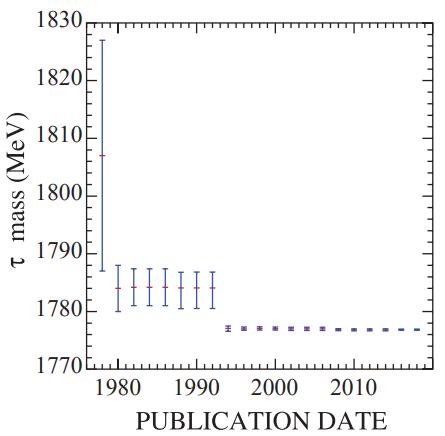
\includegraphics[width=13.5cm,height=8.6cm]{./figures/tau-mass-pdg.png}
%\caption [Mesures de la masse du Tau depuis 1978]{\textit{Mesure de la masse du Tau d'apres Particle Data Group 2019} - Tracé historique.} 
%\label{fig:7:figure7}
%\end{figure}



La seconde figure \ref{fig:7:figure7} publie par \cite{Tanabashi} concerne la masse du Lepton Tau. Cette particule inattendue est toujours inexpliquée par la théorie standard, mais Koyde a trouvé une relation simple permettant de prédire sa valeur, ce qui survint à un moment où la mesure fut corrigée de 3 sigma ( l’écart type représenté par la demie-longueur des traits). On remarquera que l’échelle des masses est donnée en MeV, qui est une unité d’énergie, est la coutume maladroite, alors qu’il est clair, selon la relation de Koide qu’il faut prendre la masse de l’électron comme unité. 

Le comble est ainsi atteint. Comme la relation de Koide ne reçoit aucune interprétation théorique dans le cadre du modèle standard, on l’ignore. Certains évoquent même le hasard. Sa validité sera justifiée dans le chapitre 8 dans le domaine - indiscutable- du milliardième. 



\subsection {scandale dans la mesure de G}
Vers 2014, les mesures de la constante de Newton G étaient contradictoires. Les plages d’incertitude des mesures des différents labos ne se recouvraient pas, elles ne convergeaient pas vers une valeur précise, voir la figure \ref{fig:8:figure8} \cite{Wu}.
 Alors le CODATA commit l’irréparable : ce comité présenta la valeur moyenne entre ces mesures comme la valeur officielle de la constante G.
La suite était prévisible : plusieurs laboratoires ont confirmés cette valeur. Le chapitre 8 indique la bonne valeur, qui est compatible avec les mesures plus sérieuses, celles de Terry Quinn au BIPM. Mais la domination américaine a encore frappé, et ces mesures furent purement et simplement oubliées, tout en reconnaissant officiellement qu’on ignore d’où vient l’erreur.
Le lecteur attentif voit très bien d’où vient l’erreur. 


%\begin{figure}
%\centering
%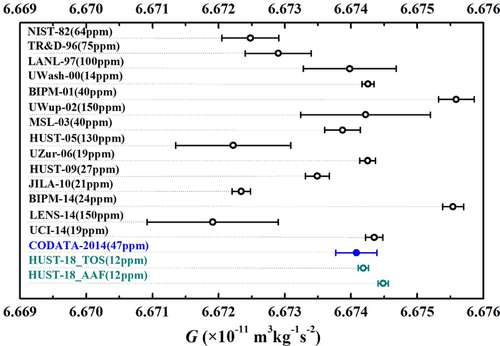
\includegraphics[width=14.5cm,height=8.6cm]{./figures/ProgressinPreciseMeasurementsoftheGravitationalConstant.png}
%\caption [Mesures de la constante de gravitation G depuis 1982]{\textit{Mesures de la constante de gravitation G depuis 1982 d'apres Progress in Precise Measurements of the Gravitational Constant \cite{Wu} par Junfei Wu  Qing Li  Jianping Liu  Chao Xue  Shanqing Yang  Chenggang Shao  Liangcheng Tu  Zhongkun Hu  Jun Luo} - Tracé historique.} 
%\label{fig:8:figure8}
%\end{figure}






\subsection {La fable de l'origine humaine du réchauffement climatique entre 1975 et 2003}

L’enracinement de cette fable dans les esprits montre bien la puissance de la collusion généralisée entre les milieux scientifiques corrompus et les politiques. Une troisième mafia intervient : les média officiels.

Ceux-ci ne montrent que des endroits où la banquise recule. On oublie de parler de ceux où elle avance.

Personne ne signale que pendant la période de réchauffement (indéniable entre 1975 et 2003, mais pas depuis), on a constaté aussi un échauffement de Mars et des satellites de Jupiter et de Neptune. L’échauffement vient donc des variations du rayonnement électromagnétique solaire. Les astronomes ont relevés un nette corrélation entre ces phénomènes.

Personne ne rappelle que le fameux « comité d’experts » le GIEC, a abandonné, en toute discrétion, le faux schéma initial qui avait lancé le mouvement.

L’analyse des carottes polaires a montré que lors des grandes variations paléo-climatiques, l’augmentation de gaz carbonique suivait et non précédait les augmentations de température, et provenait d’un dégazage des océans.

De toute façon le gaz carbonique joue un rôle négligeable dans l’effet de serre, beaucoup moins efficace que celui de la vapeur d’eau.

La raison de cette folie ? Elle se cache derrière les 3 mafias ci-dessus, une quatrième mafia : la Finance.




\subsection {Folie collective dans la dérive des continents}

\subsection {Conclusions sur le Système scientifique}

\subsection {Notes du chapitre 7}

\subsubsection{La dérive formaliste}

Préfigurant le schisme désastreux des mathématiques formelles, Napoléon transforme en 1802,  l'école 
polytechnique en école militaire à dominance mathématique. C'est le début de la décadence militaire française.

1880 : Cantor introduit les classes d'infinis, c'est le début de la théorie des ensembles et des maths formelles, par opposition aux maths intuitionnistes (Poincaré, Kronecker, Bouwers,Arnold).

1900 : Hilbert encense Cantor et propose 23 problèmes, le 6ième étant rien moins que l'axiomatisation de la physique !

1905: Poincaré publie la Relativité (Lorentz, Whittacker). Hilbert en fait signer une version par Einstein (Leveugle 2002).  

1910-13 : Bertrand Russel et Alfred Whitehead : Principia Mathematica : 1+1 = 2 démontré en 160 pages ! 

1916 : Einstein copie la Relativité Générale de Hilbert, prisonnier de l'affaire 1905.

1922 Le Nobel est attribué à Einstein pour le concept désastreux de 'photon baladeur'. 0 prix Nobel pour la Relativité.

1924 : De Broglie applique à la matière la catastrophique dualité onde-particule d'Einstein. L'aspect ondulatoire de la matière fut confirmé, mais il fallait préciser que ''tout se propage par ondes et se receuille par quanta''. Du coup, on rate que la matière est une oscillation matière-antimatière (Sanchez et al 2011) : on recherche vainement l'antimatière.

1927 : Des normaliens (groupe Bourbaki) reprennent la logique mathématique, voir la critique de Vladimir Arnold.

1929 : Hubble, influencé par l'atome primitif de Lemaître, prétend 'découvrir' la récession des galaxies, en retrouvant l'estimation (fausse d"'un facteur 7) de Lema\^itre. Einstein, au lieu d'y voir l'effet de son terme répulsif ('constante cosmologique'), admet l'interprétation du Bang, et rate ainsi la prédiction essentielle de l'accélération de la récession.

1930 : Partant de la Corrélation des grands nombres, Eddington réfute le Bang en évaluant correctement le rayon de l'Univers par un calcul élémentaire statistique. Par contre, Dirac s'accroche au Bang et introduit une variation de la constante G. Dicke en déduit une nouvelle théorie de la gravitation et propose que la Corrélation est liée à l'âge de l'Univers (principe anthropique faible). Dirac introduit l'antimatière mais pas l'oscillation matière-antimatière.

1932 : Von Neumann croit démontrer la complétude de l'interprétation probabiliste de Bohr-Heisenberg-Born en Physique Quantique, niant l'existence de variables cachées, contrairement à Einstein qui soutient que 'Dieu ne joue pas aux dés'. Mais Einstein s'accroche à la vitesse-limite de la lumière, ratant l'existence du sous-monde tachyonique.

1951 : Bohm démolit le théorème de Von Neumann. De Broglie revient à sa 'double solution', entretenant la confusion.

1965 : Dicke publie à la une du New-York Times que le rayonnement de fond est la trace refroidie du Bang.

1970-80 Le fond montre un spectre d'équilibre thermique, signe évident de Permanence, Les banguistes sont incapables d'expliquer ne serait-ce que son homogénéité : ils introduisent l'inflation. Mais le problème de l'antimatière demeure, car son élimination lors du Bang exige qu'on sorte de l'équilibre thermique (une des '3 conditions de Sakharov').

1990-2010:  Les théoriciens des cordes débouchent sur une multiplicité énorme de solutions. Les banguistes invoquent le Multivers comme épicycle ultime, soutenu par une majorité, mais contesté par Paul Steinhardt, David Gross ...

Le schisme formaliste a fait éclater les disciplines. Dès 1930, Kurt Godel avait ridiculisé les formalistes. En outre, ceux-ci ont relié les séries de Riemann avec les nombres premiers sans s'apercevoir que le 137 apparaît comme un monstre dans la plus simple des séries, la série harmonique des égyptiens, clairement illustrée dans la salle Hypostyle de Karnak. De plus 137 apparaît dans la série de Catalan-Mersenne, le terme suivant donnant le rayon de l'Univers à 0.6\% près (Sanchez, College de France 2004), montrant que la Compréhension antique était plus 'sensée' que le Savoir officiel moderne. Dés 1910, Arthur Haas avait calculé le rayon de l'atome, 3 ans avant Bohr, préfigurant l'oscillation matière-antimatière, calcul impliquant le rayon de l'univers visible par simple symétrie électricité-gravitation (Sanchez 2016). Cela confirme l'approche statistique d'Eddington, et rétablit la cosmologie permanente de Hoyle, Gold et Bondi (1948), dont l'apparition continue de matière fut généralement mieux acceptée que le brutal Bang, avec prédiction de l'accélération de la récession galactique et de la criticité de l'Univers. Le boudhiste Matthieu Ricard, dans son ouvrage avec Trinh Xuan Thuan (p. 83) \footnote{L'infini dans la paume de la main. Du big bang a l'éveil, avec Matthieu Ricard, Ed: Nil/Fayard, 2000}, retrouve le Bang Permanent (Sanchez et al, 2011), montrant que la Philosophie n'est pas séparée de la Science, (Sanchez, CEP, 2017). La théorie bosonique des cordes, écartée en raison de son caractère tachyonique, est réhabilitée (Sanchez, Springer 2017, 2018 à paraître) : le Multivers disparate officiel doit être remplacé par le Cosmos, l'élément oublié (appelé 'variables cachées') par un siècle de réductionnisme, et qui se manifeste par le rayonnement de fond.
















\subsubsection {le catastrophique systeme officiel d'unités}

 Alors qu'au moyen Age, la diversité des unités générait la plus grande confusion dans le commerce et autres activités humaines, on pourrait croire que ce genre de problème est réglé de nos jours. Loin s'en faut   : l'anarchie règne toujours.
 

Le système international d'unités est inutilement compliqué. Il en résulte que les diverses discipline utilisent en pratique leurs propres unités, un frein pour  une Science unifiée. 


C'est ainsi qu'une mission martienne a échoué pour cause de confusion entre le mètre et le mile, tandis qu'un avion de ligne s'est trouvé en plein vol à court de carburant après confusion entre litre et gallon.

\subsubsection{l'éclatement recherche-enseignement}

Mais le plus grave c'est que cette gangrène sévit même et surtout en physique, car le système S.I. officiel est tellement idiot que les chercheurs ne l'utilisent pas. Personne ne signale ce terrible dysfonctionnement de la Science, d'où la persistance du S.I dans ses coupables, néfastes et ridicules errements.


Dans plusieurs Écoles d'ingénieur, des étudiants ont poursuivi en justice certains professeurs venant de la recherche scientifique, et qui donc n'utilisent pas le système S.I. Comme les USA contrôlent la Recherche, cela ne les encourage nullement à adopter le système métrique, utilisant même cette spécificité à des fins commerciales.


\textit{Les aberrations du S.I. provoquent une césure fatale entre recherche et enseignement.}

Beaucoup d'élèves se plaignent que la Physique est incompréhensible. Il faudrait déjà réconcilier l'enseignement et la recherche. Mais il faut d'abord pour cela définir les grandeurs fondamentales. Déjà, les théoriciens ne sont pas d'accord entre eux. 

\subsubsection{le nombre des entités fondamentales}

Un débat portant sur le \textit{nombre de constantes fondamentales} a opposé récemment trois théoriciens, qui ont identifiés ce nombre avec le nombres d'entités indépendante (masse, longueur, temps, ...?). 

Le russe Lev Okun défend la position conforme au sens commun, il y a trois entités fondamentales: la masse, la longueur et la durée, la célèbre trilogie M,L,T. L'italien Gabriele Veneziano soutient que deux suffisent, tandis que Duff prétend que ce nombre peut être quelqonque, comme les sept grandeurs universelles du système international, et peut être réduit à zéro. 

Ainsi Planck, en suivant Boltzman, a ajouté le concept de température comme fondamental. Mais la pseudo-cosntante de Boltzmann, loin d'être une constante cosmique est complètement arbitraire: ce n'est qu'un convertisseur d'unité Energie-Température. Bien qu'elle figure sur sa tombe de Boltzman, elle n'a rien de fondamental, elle dépend de la définition du Kelvin, donc de certaines propriétés de l'eau.

Nous avons montré que, une fois de plus, c'est la loi du plus simple qui prévaut, puisque \textit{l'analyse dimensionnelle ternaire M,L,T, donne la longueur critique, le demi-rayon de Hubble}. Mais Okun commet l'erreur fatale d'identifier le nombre d'entités fondamentales avec celui des grandeurs fondamentales. Ainsi il ne considére pas la masse de l'électron comme une grandeur universelle.



\subsubsection {Lettre de Rémy Chauvin à Maurice Allais}

" Il y a plus d’un demi siècle que je me bat dans la même direction, sans aucun succès d’ailleurs ; j’ai fait partie des Comités du CNRS comme tout le monde ; j’ai mesuré la pusillanimité et, tranchons le mot, la lâcheté de beaucoup de collègues. Les universitaires ne sont pas des héros, on le sait depuis longtemps ; mais tout de même ! non pas la déviation des normes mais même la plus légère suspicion d’une telle déviation peut ruiner une carrière. 

Je voudrais prendre un exemple précis : le système des censeurs ou des " referees " comme on dit. J’ai appartenu au conseil scientifique d’un journal international dont j’ai démissionné pour la raison suivante : un auteur s’était plaint à moi du refus d’un article dans ledit journal, article que je trouvais fort bon ; j’interviens auprès du rédacteur du journal, qui me répond qu’on ne peut discuter la décision du censeur, par ailleurs anonyme ; j’ai démissionné tout de suite de mon poste au conseil de rédaction, en prétextant que dans ces conditions je ne voyais pas à quoi je servais. 
Qu’il existe une censure anonyme et toute-puissante, mes amis journalistes ne voulaient pas le croire " on s’est fait tuer contre ça jadis " m’ont-ils dit.


C’est évidemment la porte ouverte à toutes les lâchetés et aux vengeances personnelles. Ce système invraisemblable a été inventé par les américains qui pourtant en connaissent l’imbécillité. Il y a eu des histoires savoureuses ; un malicieux gredin a présenté à " Nature " un article qui avait été publié plusieurs années auparavant venant d’un labo prestigieux, mais il avait changé le titre, le nom de l’auteur et la provenance ; l’article a été refusé : il a donc montré que les articles n’étaient souvent même pas lus, s’ils venaient d’un labo prestigieux et non plus s’ils venaient d’un labo qui ne l’était pas. Le censeur regardait seulement le nom du labo, pour accepter dans le premier cas et le refuser dans l’autre. La même blague a d’ailleurs été refaite deux fois pour d’autres journaux, ça marche toujours.


Ce système est propre à la science. Il soulèverait les plus graves objections partout ailleurs. Un grand journal américain (Journal of Scientific Exploration) l’a d’ailleurs compris. Il accepte un article, mais il va en publier à la suite la critique, et la réponse de l’auteur à la critique ; comme cela personne n’a plus rien à dire. Mais je crois l’exemple à peu près unique.
Ou allons-nous ? La recherche biologique française (à part la biologie moléculaire) est souvent dans un état lamentable, à cause de systèmes vicieux et de la prédominance absolue des mandarins (j’en fus un, sans nulle vanité). 


\subsubsection{ Lettre Ouverte Recommandée A.R. à la Direction du CEA  }

13 Février 2001. Chacun est conscient de l’importance d’un nouveau type de communication entre le Public et le Monde Scientifique. C’est un domaine dans lequel j’ai moi-même investi 15 ans (1975-1990) où j’ai assuré quelque 150 stages de formation Laser, dans le Cadre de la Formation Permanente du CEA, au lieu de sombrer dans le ridicule " Publish or Perish "…

Ce qui a été essentiel dans cette démarche c’est que la Pédagogie était délibérément orientée vers le maillon " en principe " le plus faible de l’auditoire. Ainsi, à Pierrelatte, lors de l’importante réorientation des personnels vers les technologies de séparation isotopique par laser, on me demanda s’il était souhaitable de prévoir des " niveaux " distincts… ce à quoi j’ai répondu : " vu d’avion les différences se nivellent "… 


Cette boutade signifiait que cette Formation Permanente, contrairement au schéma scolaire, n’a pas pour but de créer ou d’accentuer un phénomène de caste, mais au contraire de souder les liens d’une équipe multidisciplinaire : j’entends par là que le chercheur de pointe doit travailler à égalité avec le modeste technicien en informatique… 


La supériorité de l’efficacité allemande provient pour beaucoup de cette autre façon, non militaire, d’aborder le travail de groupe… La confrontation qui s’annonce avec l’Europe naissante entre ces deux conceptions radicalement opposées ne peut avoir qu’une issue : la déconfiture totale du système de caste militaire français, et les historiens pourront enfin comprendre les raisons profondes, évidentes pour un pédagogue, de la décadence française…


 Les bars des sciences ne sont que les vitrines d’un système dogmatique et corrompu.  
Il est maintenant impératif d’organiser des débats sur le fonctionnement même du système scientifico-médical.


Note 3 Alerte de Halton Arp
Voici le cas d’un alerteur qui appartient au Système Scientifique et qui le dénonce de l’intérieur. Halton Arp est diplômé de Harvard (1949), puis Caltech (1953). C’est un ancien assistant de Edwin Hubble. Il a travaillé comme astronome aux Monts Wilson et Palomar pendant 29 ans avant de rejoindre l’Institut d’Astrophysique Max Planck à Munich. Ses observations des galaxies et quasars sont célèbres. Il est l’auteur d’un Atlas de Galaxies Singulières (1963), de " Quasars, Redshifts and Controversies " (1987). Il fut président de la Société Astronomique du Pacifique entre 1980 et 1983… Mais ses observations furent considérées comme " trop dérangeantes " pour le modèle standard, et on lui coupa aux US tous crédits et moyens d’observation … 


Voici donc ce qu’écrit Halton Arp dans la préface de son récent livre " Seeing Red ". près avoir observé des chaines de galaxies qui présentaient des décalages spectraux différents – ce qui est contradictoire avec le modèle officiel- :


\textit{« Je considère que mes observations ont réfuté le modèle du Big Bang. Il y a maintenant nécessité de diffuser ces nouvelles observations, ce qui est normalement le rôle des instances académiques, mais qui cherchent plutôt à les supprimer ou les ignorer. Ce livre va sûrement outrager beaucoup de scientifiques conventionnels. Beaucoup de mes collègues vont être choqués. Pourquoi alors l’ais- je écrit ? C’est que chacun a le devoir de dire sa vérité, surtout quand il s’agit de sujets d’importance. Le fait que la majorité des professionnels soient intolérants nuit au développement de la science. Il leur semble qu’abandonner leur principal modèle ne peut conduire qu’au chaos.Le seul espoir est l’intervention d’interdisciplinaires, qui peuvent remettre en question les dogmes officiels, et sont tolérants avec les théories nouvelles. Je pense qu’un débat honnête est la seule solution pour débloquer la situation. »}


\subsubsection{Témoignage de Bonnet-Bideau}

Un entretien,  paru dans Le Monde du 14 mai 20121, d'un des auteurs de l'ouvrage Un autre Cosmos ? , qui s'interroge pertinemment sur la sous-détermination des hypothèses cosmologiques – ce qui signifie qu'on est obligé de rajouter des « épicycles » –, se termine par la question suivante :

Pierre Barthélemy. \textit{Dans ce livre, vous « remerciez » les astrophysiciens et les cosmologistes qui vous ont traités par le mépris... En caricaturant, on a l'impression qu'il faut accepter le modèle dominant pour avoir le droit de faire de la cosmologie et d'entrer dans la caste. Qu'est-ce que cela nous dit sur le fonctionnement de la recherche ?}

Jean-Marc Bonnet-Bidaud : \textit{Cela nous dit quelque chose de pas très amusant. Il y a de nombreux cas dans l'histoire qui montrent que, quand on s'accroche à une description, quand les pensées se figent et deviennent très peu perméables aux critiques, la science perd dix, vingt ans, voire des siècles. J'aimerais bien que la science bouge, que les débats s'instaurent, que les connaissances progressent, mais j'ai le sentiment personnel que cet aspect frigorifié ralentit l'avancée de la recherche. C'est peut-être lié à son économie : pour proposer un projet, il faut pratiquement que vous soyez sûr du résultat que vous allez trouver. Or ce n'est pas la démarche naturelle de la science : on devrait explorer et faire autant d'expériences pour invalider les concepts que pour les valider. Dans ce livre, nous voulions souligner à quel point notre conception de l'Univers est fragile. Le modèle du Big Bang nous sert de colonne vertébrale et je n’ai rien contre. Cette façon de penser l'Univers dans sa globalité et son évolution était un bon excitateur de neurones au départ. Mais cela fait sans doute vingt ou trente ans qu'on aurait dû s'apercevoir qu'on est sur une forme de fausse piste. Quand cela ne marche pas, il faut regarder ailleurs, mais trop peu d'efforts sont faits dans cette direction. On ne veut pas trop aller dans l'inconnu et il faudra sans doute des découvertes fortuites très fortes pour faire basculer les choses. Je serais un jeune chercheur, je serais moyennement enthousiaste à l'idée de me lancer dans la cosmologie puisqu'on nous dit que tout est trouvé. Cela me fait penser à lord Kelvin qui prétendait, à la fin du XIXe siècle, qu'il n'y avait plus rien à découvrir en physique et qu'on allait seulement raffiner des décimales. C'était juste quelques années avant l'arrivée de la relativité et de la mécanique quantique.}

\subsubsection{"Expertise" anonyme sur la découverte du rayon de Hubble} 

Nota : il pourrait s'agir de Jean-Loup Puget, directeur de recherche émérite au CNRS à l'Institut d'astrophysique spatiale (CNRS/Université Paris Sud). %% \footnote{voir https://fr.wikipedia.org/wiki/Jean-Loup_Puget}

Face aux plaintes de l’auteur, qui s'étonne d’être rejeté à cause du conservatisme de la communauté scientifique face à ses idées hétérodoxes, j’ai tenté de lire son article, mis j’ai dû très vite me rendre compte que les critères habituels pour juger de la qualité d’un travail scientifique étaient inopérants.

L’auteur en effet se livre à des considérations numérologiques ; certes il y a de nombreux précédents dans l’histoire des sciences : en combinant différentes grandeurs on en fait apparaître une autre, à priori sans connexion avec celles que l’on a utilisé, et l’on conclut que cela ne peut être une coïncidence. L’auteur définit donc une longuer de Hubble, et pour ne pas utiliser la vitesse de la lumière « puisque cette vitesse est très faible par rapport à la vitesse requise pour traverser l’univers observable en un temps typique de l’atome » (il faut noter le puisque qui n’a pas le sens usuel d’une déduction tirée d’une hypothèse), il s’émerveille qu’elle coïncide avec :

 $R = 2 \hbar^2/Gm_pm_nm_e$

où interviennent très arbitrairement les masses des protons, neutrons et électrons « particules principales de la physique atomique ». Bien entendu on aurait pu mettre tout aussi naturellement n’importe quoi d’autre, la masse du quark ou celle du soleil. En divisant la constante de Planck au carré, par celle de Newton et le cube d’une masse, on obtient bien une longueur mais l’échelle des masses disponibles est telle que l’on peut fabriquer la longueur que l’on veut. Avec trois masses on fait deux rapports de masse, c’est-à-dire qu’on a deux paramètres arbitraires, et donc beaucoup de libertés.

Si l’on poursuit on tombe au paragraphe suivant sur la remarque habituelle de ce genre de considération : cette coïncidence ne peut être due au hasard. L’auteur essaye de « l’objectiver » : « La probabilité maximale d’une telle coïncidence est dans  le rapport des logarithmes de M/m où M est la masse totale de l’univers. » L’auteur ne prend pas la peine de nous dire d’où sort cette affirmation.

Or si l’on poursuit, on constate qu’il n’est pas un paragraphe qui ne soit une suite d’assertions arbitraires, parfois absurdes (par exemple l’idée que dans un système d’unité particulier « on se prive de l’apport de l’analyse dimensionnelle »), sans jamais le moindre essai pour préciser les hypothèses et en tirer les conséquences.

Dans cette suite d’assertions, toute relation à la méthode scientifique, toute rationalité sont absentes. Aucune revue scientifique ne peut accepter de telles billevesées.



Réponse dans une lettre au Secrétaire Perpétuel de l’académie des Sciences Jean Dercourt.
CC/ Présidence de l’Institut
Présidence de l’Acaémie des Sciences
Présidenced’Orsay
Minitère de la Recherche
Ministère de l’Education
JC Pecker

Monsieur

Pouvez vous me confirmer les points suivants qui ressortent de la récente « expertise » anonyme provenant, selon vous, d’un « expert reconnu », au sujet de mon projet de Lettre « Le Grandcosmos Holophysique », en souffrance de publication depuis 17 mois.

1. L’analyse dimensionnelle c’est de la numérologie.

2. Dans le système d’unité des théoriciens,  Temps = Longueur, on ne limite pas l’apport de l’analyse dimensionnelle.

3. La Méthode Scientifique exclut l’analyse « à priori » des données expérimentales.

En vous remerciant de ces confirmations, le vous prie d’agréer les meilleures salutations d’un enseignant qui en apprend tous les jours

Francis Sanchez, 22 Avril 2003.


\subsubsection{expertise anonyme sur la demande de Jean-Claude Roynette, doyen d’Orsay} 

Au sujet du premier rapport de l’année sabbatique de Francis Sanchez (Janvier 1998). Une indiscrétion l’attribue à Jean-Marc Lévy-Leblond, qui se targue partout, dans de multiples conférences, de relier la science et la culture. Q’on en juge :

Il est difficile d’écrire un rapport sur un article dont l’approche est orthogonale à celle d’un article scientifique tel que je le comprends. Je ne critique pas le fait de se lancer dans des hypothèses non orthodoxes, mais dans ce cas, il faut être capable d’en déduire des conséquences observationnelles qui soient concurrentielles avec celles du modèle standard.

Je ne peux prendre au sérieux les résultats qui sont d’origine purement numérologique et ne s’appuient sur aucun raisonnement physique. La concordance des résultats avec l’observation est arrangée à l’aide d’hypothèses sur la microphysique qui sont totalement injustifiées. Par exemple l’auteur affirme page 2 que « la microphysique utilise principalement la masse de l’électron ». Or, s’il y a un résultat dont nous sommes certains aujourd’hui, c’est que l’origine de la masse reste un des problèmes non résolus de la physique des particules. De même aucun physicien des particules ne peut prende au sérieux l’affirmation selon laqelle « les trois particules principales sont les plus stables ». Les masses des quarks (pour autant qu’on puisse les définir) sont certainement plus fondamentales que celles du proton ou du neutron. Le fait de choisir arbitrairement certaines particules plutôt que d’autres de façon à faire coïncider les résultats numérologiques avec les données n’est absolument pas convaincant. A ce propos il est étonnant que l’auteur n’ait pas remarqué que son rapport $(p+n)/2 \approx 1852,3$ , ce qui est à mieux de $10^{-3}$, la valeur du mille marin en mètres. Cette coïncidence ne me semble pas moins profonde que celles remarquées par l’auteur.    



\subsubsection{Trois cas de censure académique}

Voici 5 cas exemplaires de la médiocrité, de l’obscurantisme et de la répression de la pensée qui gouvernent actuellement la recherche et l’enseignement supérieur en France. La vraie recherche, celle qui ne sait pas à l’avance ce qu’elle va découvrir, ne serait-ce qu’une impasse épargnant aux suivants une perte de temps, se heurte à la conception officielle, qui croit avoir ce qu’il convient de découvrir. Et aucune discipline n’es épargnée. En fait, tout chercheur, tout enseignant est libre en France, sauf de contester le darwinisme, le génie d’Einstein, la Relativité, le Big Bang et autres dogmes scientifiques en matière d’énergie nucléaire, de biologie, de santé publique, d’économie etc...  

Fabienne Wolff-Bacha a soutenu en 1997 une thèse sur le sujet suivant « Siulation de transmutation de déchets nucléaires à vie longue ». Sujet actuel et crucial s’il en est. L’EDF avait par contrat subventionné les premières années de cette recherche. Malheureusement, Fabienne avait pris le mot « recherche » au sérieux et s’est trouvée contrainte, à la fin de son travail, d’infirmer, sans même le soupçonner, les conclusions qu’on attendait d’elle. Elle a perdu son contrat et a dû s’inscrire à l’ANPE pour terminer sa thèse. Bien qu’elle ait satisfait à toutes ls démarches, le CNRS a rejeté sa candidature au prétexte qu’elle avait plus de 24 ans. Sommé de démissionner, son directeur de thèse a refusé. On l’a alors muté d’office dans un placard à Orsay. Le « groupe de calcul parallèle »  qu’il dirigeait a été dissous, son matériel informatique confisqué de nuit, câbles coupés pour faire plus vite. Fabienne résumesa recherche et l’agression dont elle est victime dans un texte publié sur le forum du sénat.

Bernard Dugué, diplômé de l’Ecole des Mines de Saint-Etienne, docteur en pharmacologie, a exercé les fonctions de Maître de Conférences à Bordeaux. Au terme de ses tros années de stage, il a été licencié pour avoir entamé de sa propre initiative des travaux en biologie théorique et l’avoir malencontreusement fait savoir., notament en mentionnant un projet d’article dont la qualité fut remarquée par René Thom, alors président de la société française de biologie théorique. Suie à cet événement et face aux difficultés tant morales que matérielles, il poursuit ses recherches, publie ses travaux théoriques, en avance de dix ans puisqu’il anticipe la nécessité de faire appel à la théorie quantique our comprendre la complexité du vivant. En suite il écrit un long mémoire présentant sur 600 pages une esquisse de système métaphysique. Ce travail est remarqué par cinq universitaires qui lui accordent le doctorat de philosophie. Il publie ensuite une représentation de son système en le recadant dans une perspective ontologique et historique (« l’Expressionnisme, prolégomènes à une métaphysique des temps nouveaux, l’Harmathan, 1998 »). Malgré son profil transdisciplinaire, son niveau bac+21, sa quadruple compétence en « sciences dures », sciencesbiologiques, théorie des systèmes et philosophie, son dossier est rejetté d’année en année par les commissions d’universitaires, peu disposées à tolérer l’originalité affirmée et l’innovation intellectuelle.

Francis Michel Sanchez enseigne normalement la physique à Orsay. Il a d’autre part l’habitude rédhibitoire de se poser des questions d’ordre philosophique et d’émettre des doutes, études à l’appui sur la théorie du Big Bang. Pour cette seule raison, il n’a jamais été nommé professeur. Ses travaux sur la cosmologie ont été rejetées sur la base d’expertises anonymes, en contradiction avec des avis favorables dûment sgés par des spécialistes tels que Pecker. Un beau jour un professeur vertueux a fait irruption dans ses TP à Orsay et lu a interdit de pzrler de ses recherches dans un module d’orientation. Depuis lors sa hiérarchie tente de lui interdire d’enseigner, en ne lui attribuant aucune affectation. Il est le fondateur d’une nouvelle discipline, l’holophysique, qui se propose d’unifier tous les champs scientifiques. Certains résultats sont directement vérifiables par un large public non spécialiste. Quoi ue l’on pense de son approche pythagoricienne, elle a au moins le mérite de relancer, à propos de la méthode scientifique, une controverse malheureusement perdue dans le brouillard de la médiocrité et du talibanisme général qui caractérise la pensée actuelle. Francis plaide pour une charte scientifique inexistante dans le système actuel dont l’effondrement lui semble inéluctable.

\subsubsection{De l'Optique au Cosmos}

Francis Michel Sanchez sort major de l’Ecole Supérieure d’Optique en 1969 et entreprend une refonte totale de l’Optique, en reprenant à la base les expériences fondamentales avec les élèves-ingénieurs de l’ESO, qui le désignent spontanément comme leur meilleur enseignant. Il présente une thèse d’Etat en 1975 sur la cohérence d’ordre supérieur du laser dont il a lui-même défini le thème et le déroulement, et dans laquelle il introduit un nouveau concept, " l’holographie temporelle ". Il participe alors de façon massive à la Formation Permanente des personnels (150 stages), dans laquelle il privilégie l’approche vraiment scientifique au détriment de l’approche scolaire. Il perfectionne et révolutionne les techniques holographiques à tel point qu’il réalise en 1987 un hologramme en couleur infalsifiable de 1 mètre carré avec un faisceau laser de 1 mW. Cette performance est tellement extraordinaire et révélatrice qu’il entreprend d’étendre le " Principe Holographique " à toute la Physique. L’idée est que la Nature conserve toute l’information, ce qui pourrait enfin unifier la Physique avec la Biologie et la Cosmologie…En particulier, l’expansion de l’Univers dans un GrandCosmos s’explique alors simplement, en assimilant la Matière et l’Espace à des mémoires saturables, ce qui présente l’ADN sous un jour nouveau… Il trouve dès 1994 des corrélations de type holographiques entre les Paramètres libres du Modèle Standard, ces nombres purs dont aucune mathématique connue ne rend compte, et présente à Cambridge son " Holic Principle ", qui veut que l’Univers se recalcule lui-même à chaque quantum de temps. Il est systématiquement censuré de publication en France, en particulier par la fondation de Broglie et l’Académie des Sciences où seul l’astrophysicien Jean-Claude Pecker devine l’importance de ses travaux. Dans le même temps, coïncidence bizarre, le prix Nobel t’Hooft publie aussi un " Principe Holographique ", mais sans savoir vraiment l’utiliser et réaliser qu’il réfute le modèle Standard du Big Bang, ce qui explique que tout le système universitaire rejette les travaux de Sanchez, qui les publie donc, à partir de 1999, sur l’Internet où il ressort que sa théorie rejoint la Théorie Fondamentale d’Eddington, le fameux physicien qui avait été critiqué dans les années 30 pour avoir osé relier les paramètres libres avec les paramètres cosmologiques… Seul Chadraseckar reconnaît qu’Eddington avait préfiguré les algèbres qui apparaissent maintenant dans la Théorie des Cordes, dont la série particulière 2 + 4p apparaît nettement dans le fameux " Axe Topologique " de Sanchez, où les données de la Microphysique se prolongent harmonieusement vers celles de la Cosmologie, confirmant l’avancée d’Eddington… Le faisceau de recoupement est tel que Sanchez prévoit scientifiquement que l’expansion doit être de type exponentiel (de récentes observations confirment effectivement une accélération) et que le fond de l’Univers doit être froid (2.7 Kelvin) et non chaud comme le veut la théorie officielle du Big Bang… Il s’agit là d’une prévision cruciale qui montrera à tous que le système scientifique a déraillé depuis les années 1930.


\subsubsection{Les pères de l’astrophysique française Shatzman, Pecker et Audouze}
        Ce sont les deux normaliens Evry Schatzman et Jean-claude Pecker qui relancèrent, en 1945, l’institut d’Astrophysique de Paris. 
         En bons normaliens il commencèrent par rédiger un traité Astrophysique Générale. D’après Schatzman, c’est ce qui a retenu Pecker qui voulait partir aux USA. 
            Dans la tradition normalienne toujours, ils se sont attaqués à des problèmes mineurs, Shatzman pour l’étude du coeur des étoiles, Pecker pour celle des atmosphères stellaires.

Heureusement Pecker révèle assez tôt son intérêtpour la cosmologie : on lit dans son auto-biographie : « Je dois dire ici l'intérêt très vif que j'ai pris dès les années cinquante au débat cosmologique auquel j'ai consacré de nombreuses publications. J'ai régulièrement exprimé des doutes sur le modèle standard (dit du « big bang ») et suggéré des solutions alternatives, mais partielles. Je continue à penser que l'on est loin d'une solution cohérente des problèmes cosmologiques. »

C’est seulement pour cette raison que Pecker a émis un avis positif sur la découverte 3 minutes de la longueur critique de l’Univers par Sanchez. L’Université d’Orsay eut à choisir entre ce rapport signé de Pecker, et l’expertise anonyme ridicule attribuée à Lévy-Leblond.

Mais dans son rapport Pecker étale son ignorance de la physique fondamentale : il y déplore que cette longueur est la moitié du rayon de Hubble, alors que c’est bien R/2 qui est la distance critique. Par la suite il m\^elera le nom de Sanchez avec celui d’un numérologue, prouvant par là qu’il n’avait rien compris à ce pilier de la  physique qu’est l’analyse dimensionnelle.

Pecker était un mondain. Quand il accepta d’être secrétaire de l’International Astronomical Union, un collègue l’avait prévenu : sa carrière de chercheur s’arrêterait là. Mais, suite à ses nombreux déplacements dans le monde, il rencontra ainsi beaucoup d’astronomes, en créant des liens d’amitiés. Ce fut le cas avec Valery Kotov, astronome de Crimée. Plus tard, celui-ci, avec son collègue l’astronome russe Viktor Luyty, proposèrent à l’Académie de Sciences un article sur les oscillations non-Doppler dans le rayonnement solaire et dans plusieurs quasars. Si Pecker n’avait pas été à la direction de la section astronomie des Comptes Rendus, il est certain que cette Lettre décisive eut été rejetée, car elle contrevient à la physique la plus élémentaire. Mais Pecker n’y a pas prêté plus d’attention, même après la conférence au Collège de France ou Sanchez et Bizouard ont montré que cette période définissait la valeur de la constante G avec une précision inégalée.

Bref, Pecker a été décisif, notament pour cette initiative d'organiser cette conférence, mais il n’a pas saisi l’ampleur de la découverte. Il a préféré se ranger au coté de son ami Jayant Narlikar, qui, lui, a bien senti le danger pour ses propres théories des avancées de Sanchez, et s'opposa à leur publication. Mais Pecker passa outre, et il se décida enfin, aorès 9 ans d'effort, à publier enfin la découverte.

    Schatzman fut longtemps président de l’Union Rationaliste, et a toujours prétendu vouloir défendre la Science. Il a publié en particulier « La Science Menacée », où il écrit dans la page de couverture  « Nous vivons dans un monde de douleur, de souffrance, et il n’est que trop facile d’accuser les applications techniques des découveres scientifiques. L’opinion a radicalement changé depuis des siècles : la science sert aujourd’hui de bouc émissaire, au mépris de tout un ensemblre de causes sociales, économiques, politiques, beaucoup moins visibles que les manifestaions matérielles de la technologie avancée. Combattre sur tous les fronts ce mouvement anti-science, rendre à la passion de savoir sa place dans la culture et l’éducation, faire admettre à tous, et parfois à des dirigeants parfois irresponsables, l’enjeu social de  la recherche : en un mot, donner une vision nouvelle de l’avenir de la science, tel est l’objectif de ce livre »

 Quand Schatzman fut alerté du blocage institutionnel devant la Découverte, voila sa réponse consternante  (voir doc jointe) 

Quand au troisième normalien de l’astrophysique, bien que dûment alerté, Jean Audouze, il n’a pas pris la peine de répondre.

En bref, la crème de note système éducatif, ces normaliens qui sont, de part leur formation scolaire où tout est parfaitement défini, incapables de grandes avancées, sont de plus incapables de reconna\^itre une avancée décisive quand elle se présente à eux. Ce fut le cas en particulier pour le prix Nobel Claude Cohen-tannoudji, qui s'est permis de répondre " je ne peux vous recevoir que dans 2 ans".


 
\section{Chapitre 7. 30 ans de perdus en Bio-médecine}

\section{Chapitre 8. La grande réunification}

La philosophie naturelle est ici reprise sur des bases solides. Ce sont en premier lieu les observations astronomiques, le fameux "sauvetage des phénomènes" d'Aristote. En second lieu, sont repérées les relations entre les nombres simples et les nombres mystéreux qui apparaissent en physique et biologie. De la sorte, ces trois domaines qu'on pensait séparés, l'Arithmétique, la Physique et la Biologie sont réunifiés par la simple constatation suivante : \textit{ le Cosmos calcule}

L'outil utilisé pour cette démonstration est cette merveille technologique qu'est la calculatrice scientifique. C'est l'équivalent de la lunette astronomique des temps dits modernes.

C'est ainsi que s'applique la phrase prémonitoire d'Augustin Fresnel, \textit{"Quand une hypothèse est vraie, elle doit conduire à la découvere de rapports numériques qui lient entre eux les faits les plus éloignés".} 

\subsection{La loi du plus simple}

La vérité réside dans la simplicité. Le philosophe anglais Guillaule Occam a ainsi introduit son "rasoir d'Occam", qui veut qu'entre deux solutions, il faut choisir la plus simple.


C'est le contre-pied de la démarche académique usuelle, qu'on peut résumer par "pourquoi faire simple quand on peut faire compliqué". Comme si la simplicité était repoussante. Ainsi au lieu de dire qu'un grand nombre est un petit nombre $n$ multiplié $N$ fois par lui-même, on préfère enseigner que $N$ est le logarithme à base $n$ du grand nombre. 


Ainsi le regretté Jean-Claude Pecker, le parangon de l'astronomie mondiale, qui avait accumulé une somme énorme de connaissances sur l'histoire de l'astronomie, ayant passé le plus clair de son temps dans les conférences internationales, ose écrire, page 284 dans son livre-testament "l'Univers exploré, peu à peu expliqué"\textit{"Faut-il démolir les idoles d'Occam (s'il en est), pour manifester nos réticences vis-à-vis des constructions pythagoriciennes, dont il est en quelque sorte le point de départ mental (nombres entiers, harmonies, figures simples, symétries...)?}

On  ne peut être plus clair : une aversion totale pour la simplicité. C'est précisément parce qu'il trouvait le modèle officiel du Big Bang trop simpliste qu'il a soutenu Sanchez aux prise avec son Université d'Orsay, qui plutot que d'admettre une telle révolution en cosmologie lui avait conseillé de prendre 2 ans de repos dans une maison spécialisée.


Pecker va même va jusqu'à critiquer le concept de symétrie, rejetant ainsi la physique des particules. Mais Il a oublié de mentionner dans l'extrait ci-dessus un concept qu'il a détesté tout particulièrement : celui d'analogie, voir son expertise sur le premier rapport de l'annee sabbatique de Sanchez:

Voir figure \ref{fig:17:figure17}

%\begin{figure}
%\centering
%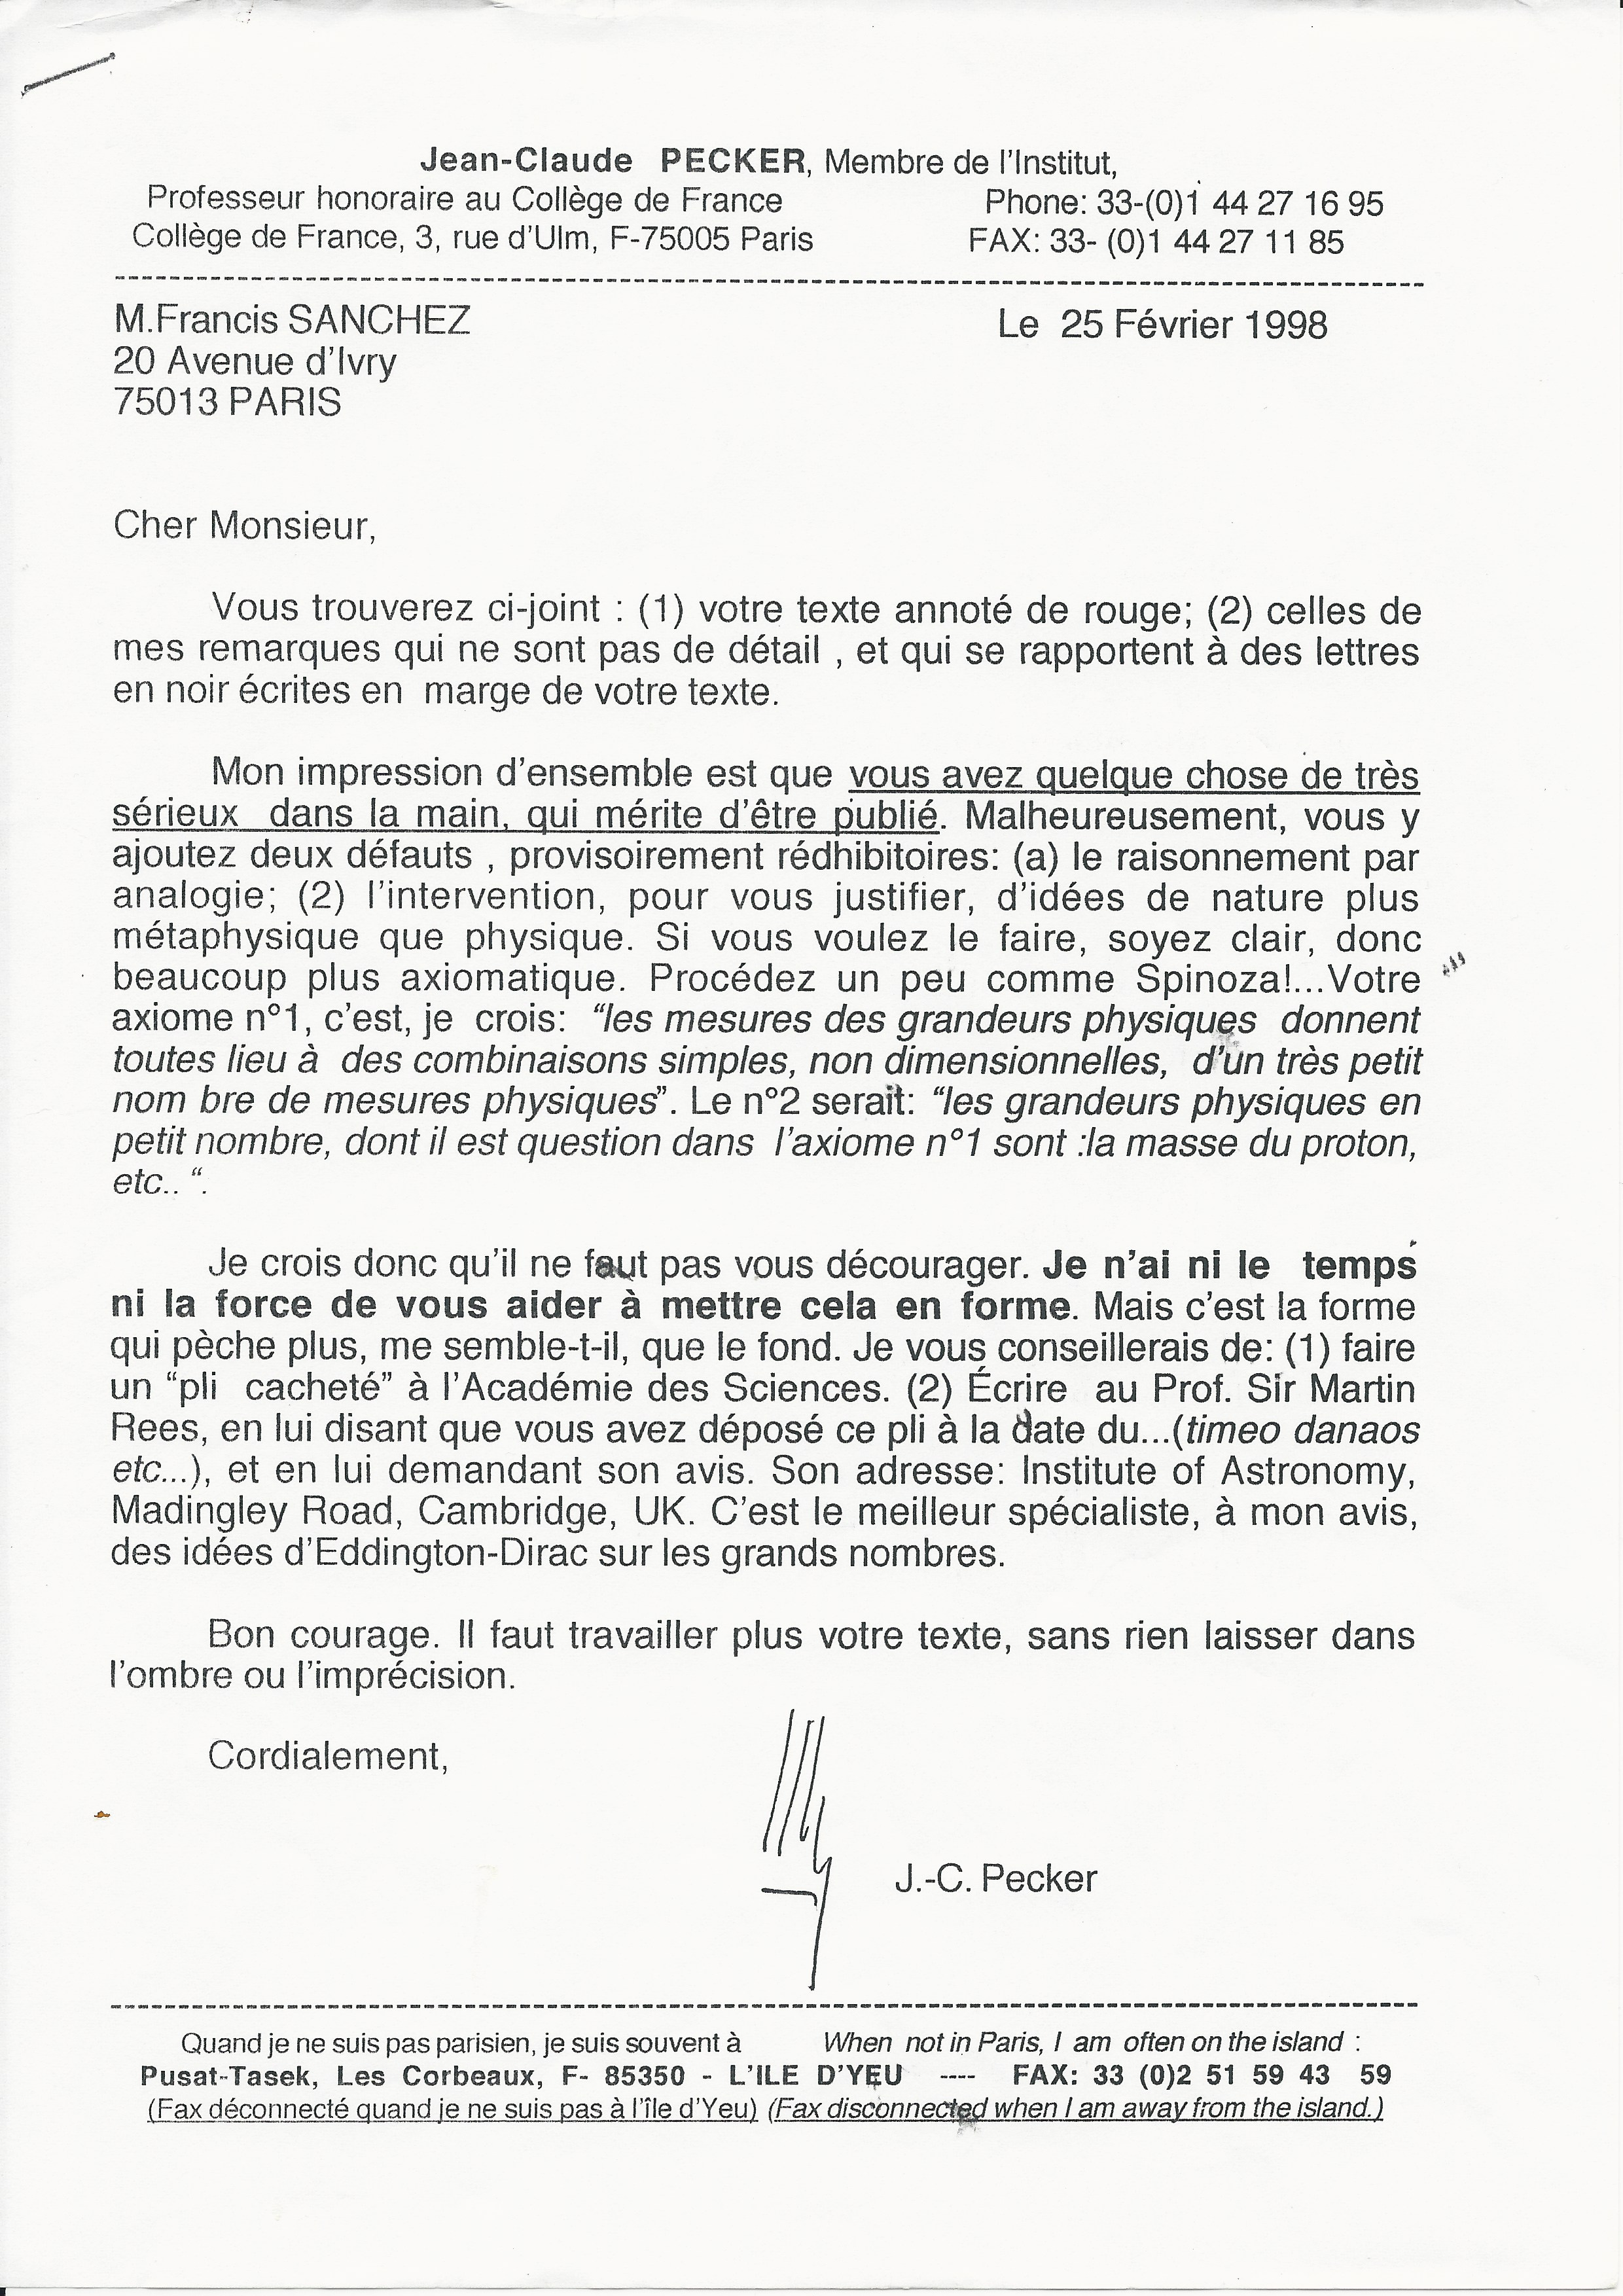
\includegraphics[width=8.5cm,height=11.5cm]{./figures/Pecker98.jpg}
%\caption [Rapport de JC Pecker évaluant le travail en cosmologie de Francis M. Sanchez]{\textit{Rapport de J-C Pecker membre de l'Institut professeur honoraire au college de France} - 25 Fev 1998.} 
%\label{fig:17:figure17}
%\end{figure}


Car Pecker n'a jamais pu admette que la simple analogie entre l'atome et l'Univers permettait de calculer le demi-rayon de celui-ci (chapitre 3). Le calcul du rayon de l'atome est le même que celui de l'Univers, sauf que, précisément, ce dernier est plus immédiat, car \textit{il est intuitif d'enlever la vitesse $c$, vitesse évidement trop lente pour assurer une cohérence cosmique.}


C'est évident, mais nul scientifque officiel ne peut l'admettre, encroe aujourd'hui : le calcul le plus simple de la physique donne le demi-rayon de l'Univers. Tout lycéen possède l'Univers dans son cartable. Mais il a fallut longuement batailler pour que wikipédia français l'admette, en Avril 2020, dans la section "analyse dimensionnelle". L'argument décisif fut que Jean Maruani avait reproduit le m\^eme calcul dans un aticle, en mentionnant Sanchez. 

Donc, si vous n'êtes pas copié, vous n'avez aucune chance d'être entendu.

Une difficulté, c'est que l'Univers visible, sans parler du Cosmos, est déjà tellement grand que beaucoup n'osent y songer. Mais, précisément, la vitesse de la pensée n'a pas de limite : elle remplace avantageusement la vitesse de la lumière. Voila la signification de ce calcul : \textit{l'Univers a un visage humain.}


Quand au rayon du Cosmos, il a fallut synthétiser sur un graphe les principales longueurs de a microphysique et de la cosmologie. Mais le résultat est sans ambiguité, et il réhabilite la théorie des cordes qu'on croyait perdue (note 1 : l'Axe topologique). Donc \textit {le Cosmos est compréhensible}.


\subsection {le Cosmos}

Le Cosmos ne peut être que la plus belle des structures. Or que constate-t-on chez l'enfant ? : il pose sponanément des questions. L'humain est donc fondamentalement un chercheur : la résolution des problèmes le fascine. Le Cosmos est donc aussi un chercher, qui s'équipe d'humains pour optimiser sa quête, comme un ordinateur s'entoure de périphériques.

Voilà la réponse à la plus fondamentae des questions "pourquoi posons-nous des questions ?' Blaise Pascal avait repéré ce fait que l'humain est caractérisé par le questionnement.

Plus connue est cette autre question " pourquoi y a-t-il quelque chose plutot que rien ?". La réponse s'en déduit : pour que le questionnement puisse se manifester.


\subsection{La vérité des nombres entiers}

Certains philosophes ont affirmé péremptoirement qu'il ne peut y avoir de vérité absolue. Pourtant, un enfant reconnaît bien que 2+3=5 est une vérité absolue.

La vérité réside donc dans les nombres les plus simples, les nombres entiers. Pas étonnant que le Monde se révèle quantifié , comme montré chapitre 3.

\subsection{L'harmonie musicale}

L'harmonie musicale résulte d'un \textit{calcul inconscient de l'âme}, comme disait Euler. En effet les rapports les plus simples interviennent en musique dans une série très simple, voir la note 2, où, les rapports entre les entiers les plus simples impliquent l'apparitions des deux principales constantes mathématiques, la base de calcul optimale $e$ et le nombre d'Archimède $\pi$, le rapport de la demi-circonférene d'un cercle à son rayon.

Ces nombres $e$ et $\pi$ ont en principe un nombre infini de décimales. Ils appartiennent à l'ensemble des "nombres réels", mais qui n'ont rien de réel. Le mathématicien Kronecker disait même "Dieu a inventé les nombes entiers, tous les autres sont des inventions humaines".

Dans la salle des mathématiques du palais de la découverte de Paris, le promeneur est invité à contempler les 700 premières décimales de $pi$. Ca donne un tournis tout-à-fait inutile et trompeur: un simple developemnt en fractions successives montre le nombre caractéristique du neutron (note 3).

En fait ces nombres ne sont que des idéalisations : aucun ordinateur ne peut faire de calculs avec ces nombres. Seules des approximations peuvent être utilisées. C'est ce que fait le Cosmos, puisqu'on retrouve aussi une constante physique essentielle dans le développement fractionnaire de $e$. 



\subsection{La voie d'Archimède}










\subsection{Le principe Holographique}
\subsection{Le Principe Holique}
\subsection{L'Axe Topologique}
\subsection{L'unification géo-dimensionnellle}
\subsection{Le testament d'Atiyah}




\subsection{Notes}
\subsubsection{l'Axe topologique}

Voir figure \ref{fig:2:figure2}.
%\begin{figure}
%\centering
% \fbox{\rule[-.5cm]{4cm}{4cm} \rule[-.5cm]{4cm}{0cm}}
%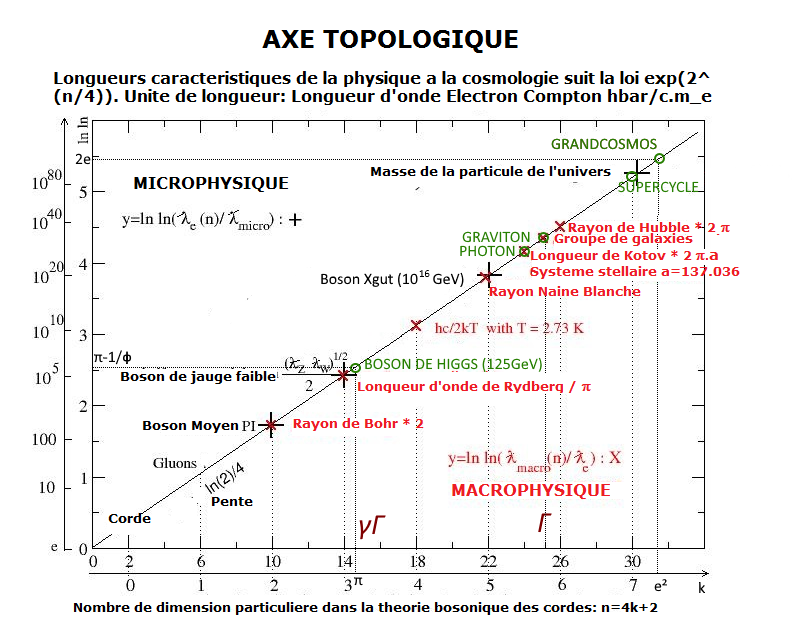
\includegraphics[width=15cm,height=16cm]{./figures/figure.png}
%\caption[Axe Topologique]{L'axe topologique. Le double logarithme naturel (y = lnln(Y)) de quantités physique sans dimensions (Y) corresponds à la corde dimensionelle de series n = 4k + 2, de k = 0 a k = 7, montrant la périodicité de Bott qui est à l'origine du nom Axe Topologique.}
%\label{fig:2:figure2}
%\end{figure}






\subsubsection{L'harmonie numérique musicale et les constantes $e$ et $\pi$}

\subsubsection{Le neutron dans le $\pi$}

\subsubsection{Le nombre hiérarchique dans la base $e$}


L'harmonie musicale résulte d'un \textit{calcul inconscient de l'âme}, comme disait Euler. En effet les rapports les plus simples interviennent en musique dans la série, où dans la gamme de Do, les notes sont respectivement Sol, Fa, Mi, Mibémol:

%\begin{equation}

%(3/2)^{2+3} \approx (4/3)^{3+4} \approx (5/4)^{4+5} \approx (6/5)^{5+6} ...... \rightarrow e^2

%\end{equation}

La constante $e^2$ est le carré de la base optimale $e \approx 2.718281828... $. Si l'on considère tous les nombres de la forme $x^N/x$ on obtient la valeur maximale pour $x = e$.


La relation musicale ci-dessus est d'autant plus précise qu'on considère une fraction plus complexe. Or cela semble violer la loi du plus simple : le premier terme doit donc révéler une importante propriété des nombres. En effet, la calculette montre que:


%\begin{equation}

%e^2 \approx (3/2)^{\pi ^2/2} 

%\end{equation}

où appara\^it la constante d'Archimède $\pi$.



\subsubsection{Transfert dimensionnel et Principe Holographique }
 
Comme nous l'avons vu, la Cosmologie permanente n'utilise pas les équations différentielles de la Relativité générale, qui doivent être remplacées par des équations intégrales, où il n'y a pas de constante d'intégration. Les plus simples de ces relations intégrales sont des « transferts dimensionnels » : on égalise des quantités géométriques de dimensions différentes, par exemple une surface et un volume.


D'où le rapprochement avec l'holographie, cette technique permettant de visualiser des scènes 3D, à partir d'un hologramme mince 2D. C'est ainsi que des théoriciens ont introduit un « principe holographique », qui apparaît comme essentiel en physique théorique.



Mais il s'agit d'un abus de langage, car ce n'est pas ce qui se passe vraiment dans un hologramme, lequel transforme une surface d'onde dénuée d'information (la surface d'une sphère) en une autre surface d'onde, mais celle-là chargée d'information (surface sphérique déformée). Cela se produit par diffraction sur des micro-strates (invisibles à l’œil) situées sur la surface de l'hologramme. 


Et comment réalise-t-on ces micro-strates ? Il suffit d'enregistrer (par photographie à grain très inférieur à la longueur d'onde dans les hologrammes optiques) les franges d'interférences entre une onde pure, sphérique, avec l'onde chargée d'information qui provient de la scène à holographier. 


C'est une technique d'une extrême simplicité, et aussi d'une grande généralité, applicable à toutes formes d'ondes, des ondes acoustiques aux brogliennes associées aux particules, mais une  technique qui exige que les franges d'interférences soient immobiles pendant la prise de vue, donc qu'une seule fréquence soit utilisée. C'est pourquoi les hologrammes optiques nécessitent un laser suffisamment cohérent, donc suffisamment monochromatique (contrairement à une opinion trop répandue, les lasers ne sont pas tous aptes à l'holographie).



Alors pourquoi parle-t-on de 3D en holographie ? C'est que la vision est liée à une reconstruction mentale 3D. Le cerveau reconstruit le volume, d'après l'expérience acquise (c'est pour ça qu'un bébé attrape tout), grâce à la vision binoculaire, puisque chaque œil voit la scène sous un angle différent, et le mouvement de l'observateur produit une variété de points de vue, mais ce, toujours à partir d'une surface d'onde 2D.



\subsubsection{Rappel sur l'holographie}

L'holographie est la ma\^itrise de l'information véhiculée par les ondes. Or comme tout se propage par onde,\textit {l'holographie est centrale en Science}. Limiter l'holographie au domaine optique est un grave contre-sens. C'est pourtant ce qu'on trouve dans l'Encyclopédie Universalis. 



Rappelons que même la matière se propage par ondes, ce qui fut une surprise totale quand de Broglie a avancé cette idée. 



L'idée de base est très simple : toute interaction est un phénomène à deux étapes : d'abord l'émission qui combine l'information ondulatoire avec une onde pure, sans information, c'est-à-dire cohérente, qu'on appelle onde porteuse. Un hologramme est ainsi formé. Ensuite, la détection utilise la même porteuse pour décoder l'information utile contenue dans l'hologramme.


C'est par exemple le principe des émissions radio à modulation de fréquence. Ainsi le récepteur radio doit disposer d'un oscillateur interne pour reproduire la fréquence qui permet d'extraire le signal utile. Dans ce cas le milieux holographique est l'espace, et l'information est déployée dans le temps.


Pour l'holographie proprement dite, l'information est déployée dans l'espace et le milieu holographique est un multi-récepteur, dont la cellule est inférieure à la longueur d'onde.


Cette idée simpliste est apparue plusieurs fois. Ainsi Mieczysław Wolfke l'a suggéré en 1920 pour les fasceaux X en cristallographie, mais ne l'a pas concrétisé \cite{Gabor}. Ensuite Dennis Gabor, désirant l'appliquer pour les ondes de la microscopie électronique, l'a développé en optique en 1947. Ce fut une surprise totale pour le opticiens. Ceux-ci n'avaient pas songé à cette technique, car ils ne disposaient d'un moyen direct pour traiter l'information optique: ce sont les instruments classiques, la lunette, le microscope.



L'histoire raconte que l'idée a germée dans l'esprit de Dennis Gabor, alors qu'il était assis dans un parc. Confronté au problème délicat du microscope électronique, où les lentilles électroniques sont de très mauvaise qualité, il s'est posé la question : peut-on faire de l'imagerie sans lentilles ? Poser la question appelait la réponse immédiate : il suffit de disposer d'une onde cohérente, comme en radiophonie. Cela anticipait le laser, voir ci-dessous.


Gabor a ajouté un concept additif : si on agrandit le récepteur d'un facteur $F$, et si l'on le démodule avec un faisceau de restitution ayant une géomtrie ( y compris la longueur d'onde) du même facteur $F$, on obtient une restitution parfaite agrandie du même facteur. Ce 'principe de Gabor' allait être très utile par la suite, et il a conduit récemment à la formulation théorique donnant les masses du photon et du graviton \cite{Sanchez}.



Mais l'holographie de Gabor présentait un grave défaut, dû au fait que la porteuse n'était pas spatialement séparée du faiscau utile. Dans un tel "montage en ligne", il se produit une onde restituée parasite qui vient brouiller l'image utile. Pour cette raison, les physiciens furent peu interessés par cette technique. Cependant, Roger l'utilisa en holographiant un seul point source, pour fabriquer un "élément optique holographique". La thèse d'Hussein El-Sum l'appliqua aux faisceau X en cristallographie. 


L'idée a été retrouvée vers 1970 par Yuri Denisyuk, en utilisant une porteuse allant en sens contraire du signal. Les effets d'épaisseur dans l'émulsion photographique ont éliminé l'image parasite, mais il n'a pu matérialiser cette technique que pour enregistrer une scène contenant une seule information : il holographia un simple miroir convexe, fabricant ainsi un autre type d' "élément optique holographique" \footnote{aussi appelé EOH ou HOE en anglais}, nettement supérieur à celui de G. L. Rogers.


La raison de cette limitation drastique en optique est que lorsqu'on extrait une onde cohérente d'une source thermique, on perd trop d'énergie. Même en partant d'une lampe spectrale, comme l'arc au mercure, et en isolant la raie verte principale, la longueur de cohérence est faible. 


Puis vint le tour des ondes radar. Car les militaires avaient beaucoup investi dans ce domaine, et, dans le laboratoire du Michigan, Emmett Leith voulut utiliser l'idée de Gabor, en se ramenant à l'optique, mais en séparant spatialemnt la porteuse de l'onde-signal, il résolvait le problème de l'image parasite. Il obtint ainsi, avec son collègue estonien Upatnieks, qui n'avait pas le droit de s'occuper des questions radar, ultra-secrètes, des images de transparents 2D de bonne qualité. L'étape suivant était de passer à l'holographie d'objets 3D. Mais la lumière diffusée était trop faible. Par un curieux concours de circonstance, c'est à ce moment précis que le labo vit arriver le premier laser à gaz Néon/Hélium. Bien que de faible puissance nominale (milliwatt), le gain en luminosité cohérente était énorme, et près d'un an pour régler le problème des franges parasites que donnait une telle cohérence, Leith et Upatnieks obtinrent les premières images holographiques.


Le succès fut immédiat, à tel point que le nouveau directeur de laboratoire, fraichement débarqué depuis l'Europe, George Stroke voulut s'approprier une telle avancée, conformément à la coutume des labos européens. Surtout que E. Leith n'avait pas encore obtenu sa thèse de doctorat. Stroke écrivit rapidement le premier ouvrage sur l'holographie, en faussant la réalité historique et milita pour que le prix Nobel soit octroyé à Gabor seul, avec éventuellement lui-même. Gabor reçut le prix en 1971, mais, dans son discours, il minimisa l'apport décisif de Leith et Upatnieks.


Dans l'intervalle trois laboratoires américains redécouvrirent par hasard la méthode à porteuse arrière de Denisyuk, qui du coup fut finalement reconnu en Russie. Quelques années plus tard, Denisyuk put enfin accéder au laser, il put alors bénéficier pleinement des améliorations décisives qu'il avait effectué avec Rebekka Protas à l'Institut d'Optique Vavilov de Leningrad pour réaliser des émulsions super-sensibles à grains très fins (0,2 microns). 


C'est ainsi que l'école russe produisit des hologrammes de meilleures qualité que les hologrammes américains et européens. En effet il suffisait d'un simple spot de lumiere blanche ponctuel pour restituer l'image alors que les autres nécessitaient une lampe spectrale puissante, voir m\^eme un laser pour les plus grands modèles.



C'est alors que l'école française reprit la main, en éliminant totalement la nécessité d'un lourd et co\^uteux banc optique, par la méthode de l'hologramme contact, et la possibilté du balayage permettant de faire de grands hologrammes avec de faibles faisceaux lasers, ce qui conduisit à la réalisation d'un metre carré avec un fasceau d'un milliwatt (Juillet 1987). Par la suite Yves Gentet \cite{Gentet} utilisa ces techniques pour obtenir les hologrammes-couleurs, les plus belles images, qui viennent compléter les célèbres images 2D en vraies couleurs de Gabriel Lippmann \footnote{Prix Nobel 1908}. 



A noter que Denisyuk s'était inspiré de ces travaux préccurseurs, qu'on ne peut qualifier d'holographie, car seule la vraie couleur est enregistrée localement, gr\^ace au bain de mercure servant de miroir en contact avec l'émulsion photographique à grains ultra-fins.


Mais à cause de ces décalages temporels, la littérature officielle ne fit pas grand cas des hologrammes restituables en lumière blanche, et les textes présentaient le montage de Leith comme indispensable. Ceci à tel point que, avec le laser Argon plus puissant, plusieurs labos ne parvinrent pas à faire le moindre hologramme: à cause du refroidissement qui faisait vibrer. Aucune mention n'était faite sur ce point essentiel : la rigidité du montage n'est nécessaire qu'après séparation des faisceaux, c'est pourquoi il est indispensable d'installer le laser sur une table séparée.


Ainsi plusieurs thèses discordantes furent développées dans les différents ouvrages, sans parler de l'emballement médiatique qui suivit. Même Gabor ne put s'empécher de faire le rapprochement entre l'hologramme et la mémoire humaine, en remarquant que chaque point de l'hologramme contient de l'information sur l'ensemble de la scène, de même que la mémoire n'est pas localisée dans une zone particulière du cerveau.


Plus fondamentalement, du fait de l'universalité de l'holographie il fallait introduire un Principe Holographique en Physique Théorique, voir plus haut.




\subsubsection{Histoire des applications de l'holographie}

Les premières applications de l'holographie remontent aux années 1960. Elles concernèrent l'optique (EOH); par la suite de nombreux domaines furent explorés et notamment dans le domaine des applications militaires (détonique, spectroscopie TeraHertz, balistique et propulseurs...) \cite{ISL}, aéronautique (aérodynamique et écoulement d'air, HUD), physique des particules et microscopie (chambres a bulles CERN), médicales, interferométrie, muséologie/archéologie (Ecu d'or de St Louis Bibliotheque Nationale), archivage (CD), crypto-holographie, Cine-holographie \cite{Bjelkhagen} ...
L'holographie s'applique a tout type d'onde; on peut compter l'holographie sismique et sonore.


\subsubsection{L'Holographie Quantique : masses du photon et du graviton}

\subsubsection{Rappel sur le laser}

L'histoire véridique du laser et de la fable du photon libre
Correction des idées (mal) reçues
F. M. Sanchez, janvier 2020

Pour marquer le 60ème anniversaire du laser, lié à tort par beaucoup au concept de « photon libre »,  voici le récit de son histoire. Elle est édifiante à plus d'un titre. D'abord pour rappeler à quel point l'Histoire officielle des Sciences peut être erronée. Ensuite, et surtout, pour montrer l'aveuglement des scientifiques officiels, le plus souvent des mathématiciens (mal) reconvertis.

On affirme que le père du laser est Einstein, en 1917. Il est vrai qu'il a mis en évidence l'émission induite (ou stimulée), contenue de façon évidente dans la formule du rayonnement thermique. Mais il a omis de préciser que c'est une amplification conforme (ou cohérente), ce qui est l'essence même du laser.

En effet, dans «Einstein, le Livre du Centenaire » \cite{French}, Alfred Kastler écrit, page 157 : Notons ici que cette émission induite a des caractères très différents de l'émission spontanée. Alors que l'émission spontanée se fait au hasard dans toutes les directions de l'espace, l'émission induite se fait uniquement dans la direction du faisceau lumineux stimulateur qu'elle renforce, ce qui lui vaut le nom d'absorption négative. De plus, la phase de la vibration émise est commandée par celle du rayonnement stimulateur et cohérente avec celle-ci. Einstein n'a d'ailleurs pas relevé ces caractéristiques spécifiques de l'émission stimulée dans son mémoire.

Mes cours laser au CEA présentent effectivement l'amplification stimulée comme un phénomène collectif dans un milieu homogène. Cette condition d'homogénéité est absolument nécessaire pour préserver la structure de l'onde, donc conserver l'information, que ce soit en absorption ou en amplification.

Quand on affirme que c'est un photon incident qui oblige le système à émettre un photon équivalent, c'est contraire au principe d'incertitude nombre/phase du photon. L'effet laser n'est pas un effet local, mais global. Kastler précise aussi ce point :

L'idée d' Einstein d'attribuer les interférences lumineuses à une interaction entre quanta lumineux s'est avérée incorrecte dans la suite. Nous savons que, dans un dispositif d'interférences, nous obtenons des franges même lorsque les corpuscules (photons ou électrons) traversent un à un le montage interférentiel. Le pouvoir d'interférer est donc une propriété ondulatoire indépendante de la densité de corpuscules. Il détermine le comportement d'un corpuscule unique, aussi bien dans le cas de la lumière que la matière .

Donc le photon n'apparaît qu'à la détection : durant la propagation ce n'est qu'une onde (appelée « photonde » dans mes cours). La confiance aveugle dans le soi-disant génie d' Eintein a généralisé ce type d'erreur. Noter qu'il a reçu un prix Nobel pour la seule découverte qu'on savait vraiment de lui, et pour cause, le « photon libre ». Le prestige injustifié d'Einstein a plongé tout le siècle dans cette errance du dualisme onde-particule. Le rapprochement lumière-matière de Louis de Broglie était correct, mais, en copiant Einstein, il commit une double erreur retombant sur une vérité : la matière se propage aussi par ondes. Mais il n'en a pas tiré la conséquence inéluctable : la matière vibre dans une oscillation matière-antimatière, et il s'enferma dans une vaine recherche de double solution, surtout après que David Bohm ait démontré que le théorème de complétude de Von Neumann ne s'appliquait pas.

Il était donc évident dès le départ que la physique est non-locale, mais Alain Aspect fut tout surpris quand on lui rappela qu'il pouvait y avoir des variables cachées non-locales : il avait défoncé des portes ouvertes. Lors de sa thèse, le normalien André Maréchal, directeur de l'Institut d'Optique, contrairement aux règles, a essayé en vain d'empêcher toute discussion avec les docteur es-sciences. Le journal Monde refusa de publier l'affaire car les contestations de l'école de de Broglie auraient nuit au sacro-saint consensus scientifique. C'est Olivier Costa de Beauregard qui a lancé cette affaire grotesque avec la complicité de Christian Imbert, qui cherchait à promouvoir l'Ecole Supérieure d'Optique qu'il dirigeait. Imbert a osé soutenir devant moi la réalité physique du « rayon lumineux ». Encore une victime du photon baladeur. Il fut tout surpris quand j'ai demandé ma rotation dans l'Université d'Orsay, ce qui m'a permis d'obtenir une année sabbatique décisive, voir ci-dessous. Un autre sommet du ridicule est Roland Lehoucq, ce normalien féru de science-fiction, qui dans une vidéo sur le « sabre laser », témoigne que deux faisceaux laser se traversent.

Revenons à la découverte effective du laser. Selon une confidence du normalien  Pierre Jacquinot, professeur à Orsay : ``nous avions le laser sous le nez depuis des années, mais vaut mieux ne pas le dire''. Que s'est-il s'est donc passé ?

Le prédécesseur naturel du laser, le maser, fut découvert par Charles H. Townes en 1954, qui les baptisa ainsi. L'initiale m signifiant ``micro-onde'', tandis que le L de « LASER » vient de l'anglais « light » \footnote{traduction de lumière}. Les autres lettres viennent de « Amplified by Stimulated Emission of Radiation ». 

La condition essentielle est d'obtenir une inversion de population entre deux niveaux d'énergie. C'est beaucoup plus difficile à obtenir dans le domaine visible qu'en micro-onde, car l'émission spontanée qui vide les niveaux est beaucoup plus rapide. 

Mais, contrairement au triage magnétique de Charles H. Townes dans le maser, Arthur Kastler obtint cette inversion de population par un moyen beaucoup plus général, le pompage optique,  C'est ce qu'a pu apprécier Charles H. Townes, en 1956, lors de son année sabbatique  chez Kastler, à l'ENS de Paris. Dés 1958, il publia l'article de base sur le laser, notamment l'utilisation de deux miroirs comme cavité ultra-simple. En 1958, il déposait le brevet du laser avec Arthur L. Schawlow, puis en Juillet 1960, Theodore H. Maiman bricolait un flash de photographie autour d'un barreau de rubis, dont les faces avaient été légèrement métallisées. Personne n'a cru que le premier laser était né, et son article fut refusé. 

L'ENS, qui favorise les mathématiques au détriment de la physique, avait raté le coche, pourtant évident. Gordon Gould avait même pris un brevet d'avance sur le laser qui n'avait pas encore été découvert, ce qui donna lieu à 30 ans de procédure pour définir les droits de chacun ! L'année suivante une dizaine de lasers apparurent dans des milieux très différents. Ce blocage provenait donc des théoriciens qui avaient exagéré la difficulté par des calculs trop savants.

Beaucoup de pseudo-scientifiques s'obstinent à affirmer que le laser est la preuve de l'efficacité de la physique quantique, et que le laser n'a pas été découvert par un bricoleur en Californie, oubliant l'exploit de Theodore Harold "Ted" Maiman. Richard Feynman est beaucoup plus réaliste : il avoue qu'on ne comprend pas vraiment ce qui se passe. Le laser en est la parfaite illustration. Et d'autres surprises suivirent, comme les effets Josephson et Hall quantique, qui conduisirent à revoir le système d'unité international d'unités.

Charles H. Townes était un découvreur-né. Après le maser et le laser, il appliqua en astronomie sa passion pour les molécules. En découvrant des molécules biologiques dans l'Espace, il devenait ainsi le père de l'astro-biologie. Il découvrit aussi des effets masers naturels dans l'Espace, et le trou noir géant au centre de la galaxie.    

La plupart des applications des lasers utilisent le faisceau fin pour des travaux de précision, mais l'application la plus révolutionnaire est celle en faisceau large, l'holographie, la maîtrise totale de l'information spatiale, qui exige un laser cohérent. Beaucoup croient que tous les faisceaux laser sont cohérents. C'est loin d'être le cas, aussi bien en cohérence spatiale (uniformité) que temporelle (une seule fréquence) comme je l'ai montré dans ma thèse sur l'effet « multiphotonique », en 1975, qui confirme que le photon ne se propage pas. En 1974, quand Michel H. Grosmann a voulu développer les applications de l'holographie, l' Institut d'Optique lui a répondu que tout avait été fait dans ce domaine. c'est ainsi que le centre des applications de l'holographie photonique se déplaça à Strasbourg.







\section{Chapitre 9. Prospective}

\subsection {Diagnostic sur l'état actuel des sciences}
\subsubsection{La domination américaine}



\subsection {Les remèdes} 
\subsubsection {Organisation de la Recherche}
La cosmologie doit occuper une place centrale
\subsubsection {Organisation de l'Enseignement}
\subsubsection {Organisation de la Cité}


\subsection {Prédictions}
\subsubsubsection{Prédictions en cosmologie}
\subsubsubsection{Prédictions en astro-biologie}
\subsubsubsection{Prédictions en mathématiques}
\subsubsubsection{Prédictions en informatique}
\subsubsubsection{Prédictions en sociologie}
Le développement de l'intelligence artificiele conduira à la traduction simultanée des quelqques 3000 langues actuelles dans le monde. C'en sera fini de l'hégémonie scientifique des USA.
Les sciences actuelles, qui fonctionnent sur le modèle américain, vont s'effondrer. 









\section{Conclusions}
\label{sec:headings}

Les récentes découvertes expérimentales en macro- et micro- Physique permettent d'imaginer un modèle d'Univers qui résoudrait élégamment les contradictions actuelles entre ces deux sous-disciplines. De nouvelles expériences (en préparation) devraient permettre de confirmer la pertinence de ce modèle face aux très nombreux autres actuellement en compétition. Nous essayons actuellement de le représenter sous forme d'un hologramme. Dans la conception de celui-ci nous avons réalisé des stéréoscopies dont l'une est présentée sur la Figure.

On y voit la représentation (étonnamment sous forme d'une droite!) de divers paramètres tant de la MACRO- que de la micro- Physique.


\subsection{Figures}

Figure \ref{fig:1:figure1} Tri-Axis: voir texte en anglais \footnote{http://www.ptep-online.com/2019/PP-57-12.PDF}

Figure \ref{fig:2:figure2} Axe Topologique.

Figure \ref{fig:3:figure3} Tableau du Cours d'holographie.

Figure \ref{fig:4:figure4} Temple de Karnak.

Figure \ref{fig:5:figure5} L'Est eclair.

Figure \ref{fig:6:figure6} Duree de vie du Neutron (s).

Figure \ref{fig:7:figure7} Masse du Tau .

Figure \ref{fig:8:figure8} Precision de la constante de gravitation G \cite{Wu}.

Figure \ref{fig:9:figure9} Oscillateur du LASER Nd3+ \cite{Lecompte}.

Figure \ref{fig:10:figure10} Systeme de controle  LASER Nd3+ \cite{Mainfray}.

Figure \ref{fig:11:figure11} Systeme de controle  LASER Nd3+.

Figure \ref{fig:12:figure12} Systeme de controle  LASER Nd3+.

Figure \ref{fig:13:figure13} Systeme de controle  LASER Nd3+.

Figure \ref{fig:14:figure14} Systeme de controle  LASER Nd3+.


\begin{appendix}

%This is the appendix section

\section{Glossaire}

Petit glossaire des expressions et termes utilisés dans cet essai.

\begin{itemize}


\item \textbf{Antimatière}(re-définition): matière qui oscille en opposition de phase avec la matière environnante (voir antiparticule ???)

\item \textbf{Axe Topologique}(néologisme): ordonnancement suivant un axe (topologique et cosmologique) des structures principales du Cosmos.

\item \textbf{Big-Bang} (redefinition): Terme utilisé pour la première fois par Fred Hoyle. Phase de reconstruction d’un univers particulaire. Dans la cosmologie cohérente il est permanent. big-bang Sujet a interpretation

\item \textbf{Big crunch} (re-définition) phase de déconstruction d’un univers particulaire

\item \textbf{Black Hole}

\item \textbf{Chaos}: Etat de chaos: ordre non ordonne

\item \textbf{Chronon}(néologisme): atome insécable de temps, entre un bang et un crunch (cf topon)

\item \textbf{Continu}: Idéalisation anti-quantique qui introduit le concept dangereux d'infini dans le microcosme.

\item \textbf{Continuum}(obsolète): idéalisation des formalistes, rendant toute compréhension impossible.

\item \textbf{Cosmologie cohérente} (néologisme) : cosmologie où tous les Univers particulaires sont équivalents. S’oppose au Multivers disparate officiel qui attribue des propriétés différentes à une série indéfinie et non observable d’univers. ???

\item \textbf{Cosmos}: ensemble de tout ce qui existe, non infini. C'est la réunion d'un ensemble fini d'Univers, chacun d'entre eux étant lié à une particule.

\item \textbf{Dé-synchronisation}: décalage temporel provoqué lors d’un déplacement, provoqué par déphasage dans le processus de reconstruction.

\item \textbf{Equation Diophantienne} équation portant sur des nombres entiers

\item \textbf{Gravitonde} (néologisme): désigne l’onde associée à un graviton, quantum d’énergie qui disparaît d’un atome émetteur pour se retrouver sur un atome récepteur après un calcul cosmique.

\item \textbf{Groupe local} : groupe de galaxies contenant la Galaxie, notre voie lactée.

\item \textbf{Gluonde}:

\item \textbf{Hol}: 

\item \textbf{Holic}: qui se rapporte au Principe Holique, simplifiant à l'extr\^eme les équations diophantiennes.

\item \textbf{Horizon Visible}:

\item \textbf{Immergence} (néologisme) Faculté du tout à expliquer les parties. S’oppose à la classique ``émergence", qui attribue à un ensemble des propriétés nouvelles, étrangères à celles de ses éléments constitutifs.

\item \textbf{Impermanence} (néologisme) : variabilité fondamentale des phénomènes, qui s'opose au concept cosmique fondamental de Permanence.



\item \textbf{Inertie} Reconstitution cosmique d’un objet et de son mouvement par rapport au Cosmos

\item \textbf{Infini} (obsolète) concept inventé par les formalistes pour simplifier certains calculs, notamment les séries. D'après l'étude de Alexandre Koyré, "Du monde clos à l'univers infini", le siècle des lumières serait caractérisé par l'introduction de ce concept d'infini.

\item \textbf{Inflation} : Dans le modèle du Bang inital, extension très rapide de l'Univers pour justifier l'homogénéité observée du rayonnement cosmique.  Cet épicycle ridicule, ce Bang à deux étages, a été adopté car c'est le seul moyen dans ce modèle pour justifier le caractère critique de l'Univers. En fait, le Principe Holographique explique directement ce caractère critique. Mais les tenants du Bang initial considérent à tort que le rayon critique de l'Univers est variable, donc ne peuvent appliquer lui appliquer le principe holographique.



\item \textbf{Intrication} (ou Non-séparabilité) : manifestation de l’ordonnancement cosmique entre les univers particulaires

\item \textbf{Matière noire} : matière qui oscille en quadrature de phase avec la matière environnante


\item \textbf{Multivers} : Dans le modèle du Bang initial, ensemble d'Univers disparates, possédant toutes les propriétés possibles. Son introduction permet de se dispenser d'opérer l'unification mathémtiques-physique. Cet épicycle grotesque s'oppose au Cosmos qui regroupe des Univers identiques. 


\item \textbf{Mur de Planck} (obsolète) : limite spatio-temporelle officielle. La cosmologie Cohérente le repousse d’un facteur $10^{61}$, résolvant ainsi l’énigme de la densité du vide quantique, $10^{122}$ fois l’énergie moyenne cosmique.

\item \textbf{Neutrons} : particules remontant l’organisation de l’Univers, en apparaissant dans les espaces inter-sidéraux, à raison de 5 neutrons par siècle dans le volume d’une pyramide.

\item \textbf{Nombre réel} (trompeur et obsolète): type de nombre inventé par les mathématiciens formalistes, mais qui interdit tout calcul pratique, donc cosmique.

\item \textbf{Nombrologie} (néologisme). Etude directe des relations entre les nombres cosmiques. S'oppose à la très répandue "numérologie" qui cherche des relations entre des nombtes arbitraires.


\item \textbf{Permanent Big bang}

\item \textbf{Photonde} (néologisme): désigne l’onde associée à un photon, quantum d’énergie qui disparaît d’un atome émetteur pour se retrouver sur un atome récepteur, après un calcul cosmique.

\item \textbf{Préscience}(néologisme): connaissances partielles hors cosmos.

\item \textbf{Principe anthropique}:

\item \textbf{Principe Conceptuel} (néologisme): Le Cosmos est ordonné suivant des lois esthétiques, compréhensibles par les humains. Il remplace le Principe anthropique officiel, mal défini et objet de graves contre-sens.

\item \textbf{Principe Cosmologique Parfait} (re-définition) : chaque Univers particulaire est globalement homogène, isotrope et invariant.

\item \textbf{Principe Holique} Idéalisation diophantienne du Principe Holographique

\item \textbf{Principe Holographique} principe expliquant la structuration du Cosmos en identifiant des variétés topologiques de différentes dimensions. Il relie l’énormité du cosmos, à partir de la quantification nécessaire de la constante d’Archimède pi.

\item \textbf{Quantinuum} (néologisme) : ensemble d’états discrets, par opposition au continuum.

\item \textbf{Rayonnement thermo-cosmique} rayonnement interne du Cosmos. Appelé CMB (Cosmic Microwave Background) par la science pré-science.

\item \textbf{Rayon critique} : rayon de chaque univers particulaire. Il s’identifie avec le ``rayon de Hubble'' directement mesurable. C’est aussi le Rayon de Schwarzschild de chaque Univers particulaire considéré comme un trou noir dont la particule est la singularité centrale.

\item \textbf{Récession galactique} : répulsion entre amas de galaxies permettant de renouveler l’Univers au profit de nouveaux neutrons

\item \textbf{Référentiel d’inertie} tout référentiel en mouvement linéaire dans le Cosmos. La pré-science était incapable de le définir.

\item \textbf{Rayon de Schwarzschild}:

\item \textbf{Science} (re-définition) : connaissance des lois du Cosmos.

\item \textbf{Tachyon}: particule se déplaçant plus vite que la lumière. Il a été exclu par la pré-science.

\item \textbf{Toponde/Topon} : (néologisme) atome insécable d’espace

\item \textbf{Trou noir} : miniaturisation d’un univers particulaire. Les trous noirs ont pour fonction d’évacuer la matière interne d’un amas galactique.

\item \textbf{Univers}: l'écume immergente du Cosmos, $10^{122}$ fois moins énergétique

\item \textbf{Univers Observable}: 

\item \textbf{Univers particulaire}(néologisme): partie de l’Univers qui construit et déconstruit chaque particule.

\item \textbf{Variables cachées} (obsolète): dans la pré-science, causes invoquées pour expliquer l’Univers. Elles s’identifient au Cosmos.
\item \textbf{Vide quantique}: partie principale du Cosmos.

\item \textbf{Vitesse absolue} : vitesse par rapport au Cosmos. La vitesse absolue du groupe local est de $620 km/s$.

\item \textbf{White Hole}
\end{itemize}


\listoftables{}   % table list
\listoffigures{}
%%\subsection{Lists}

\clearpage

\begin{figure}
\centering
%  \fbox{\rule[-.5cm]{4cm}{4cm} \rule[-.5cm]{4cm}{0cm}}
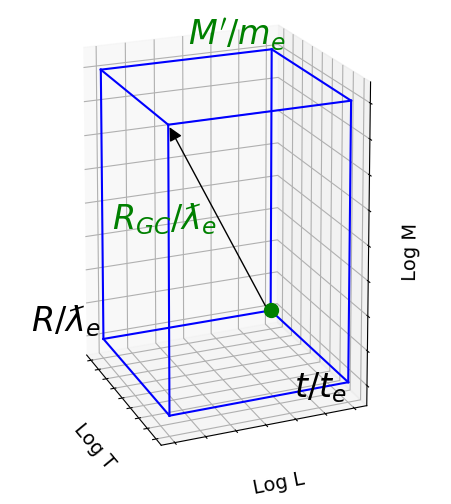
\includegraphics[width=5cm,height=6cm]{./figures/triaxis.png} 
\caption[Representation Geo-dimensionelle du couple Univers-Grandcosmos]{Representation Geo-dimensionelle du couple Univers-Grandcosmos. Dans un super espace 3D, les logarithmes naturels de temps, de longueurs et de masses sont considérés comme vecteurs. Le rapport logarithmique du rayon du grand cosmos avec la longueur d'onde de l'électron Compton fait apparaitre un vecteur normé projetant longueur et temps avec une proportion commune; le rayon de Hubble par la longueur d'onde de l'électron Compton et pour le rapport de masse; on considere $M^{\prime}$ par la masse de l'électron. $M^{\prime}$ étant la masse critique dans le Grandcosmos réduit a un hologramme spherique, ceci démontre la confirmation géometrique du principe holographique étendu (2D-1D)appliqué a l'univers d'entropie de Bekenstein-Hawking. L'existence d'un grand cosmos ne peut plus \^etre niée depuis que la relation entre $e$, $a$ et les logarithmes impliqués atteignent une précision de $10^{-7}$.}
\label{fig:1:figure1}
\end{figure}

\begin{figure}
\centering
% \fbox{\rule[-.5cm]{4cm}{4cm} \rule[-.5cm]{4cm}{0cm}}
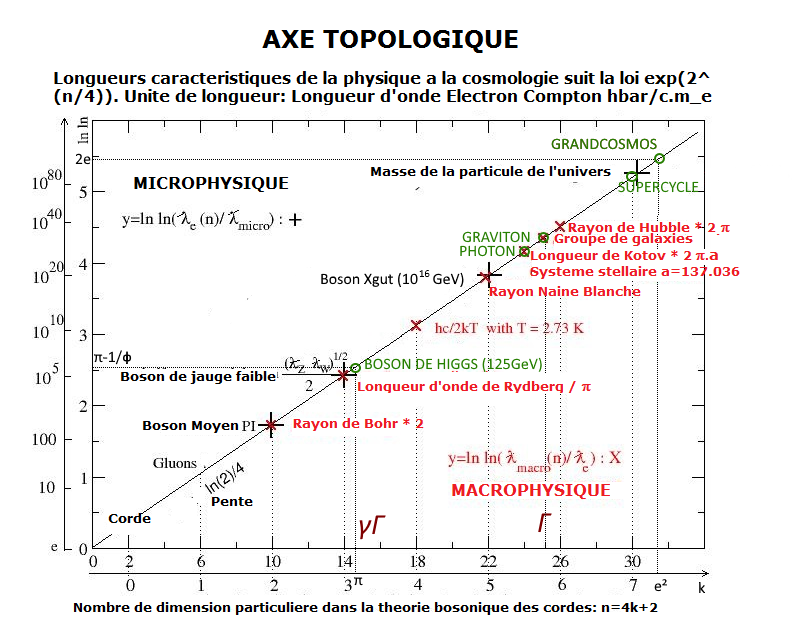
\includegraphics[width=15cm,height=16cm]{./figures/figure.png}
\caption[Axe Topologique]{L'axe topologique. Le double logarithme naturel (y = lnln(Y)) de quantités physique sans dimensions (Y) corresponds à la corde dimensionnelle de series n = 4k + 2, de k = 0 a k = 7, montrant la périodicité de Bott qui est à l'origine du nom Axe Topologique.}
\label{fig:2:figure2}
\end{figure}

\clearpage

\begin{figure}[h]
\centering
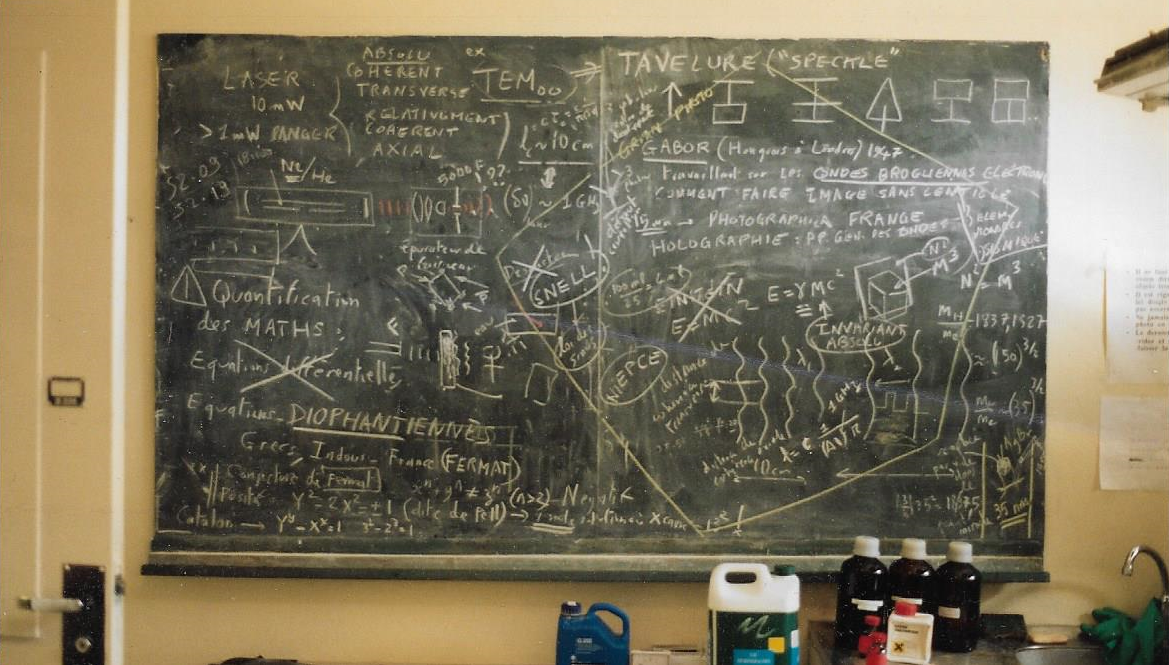
\includegraphics[width=14.5cm,height=10.5cm]{./figures/fs-tab.png}
\caption[Cours d'holographie à l'Institut d'Optique d'Orsay]{\textit{Cours d'holographie de Francis M. Sanchez à l'Institut d'Optique d'Orsay fin des années 1980}, remarquer les quelques formules ainsi que les références aux équations diophantiennes.} 
\label{fig:3:figure3}
\end{figure}

\clearpage

\begin{figure}
\centering
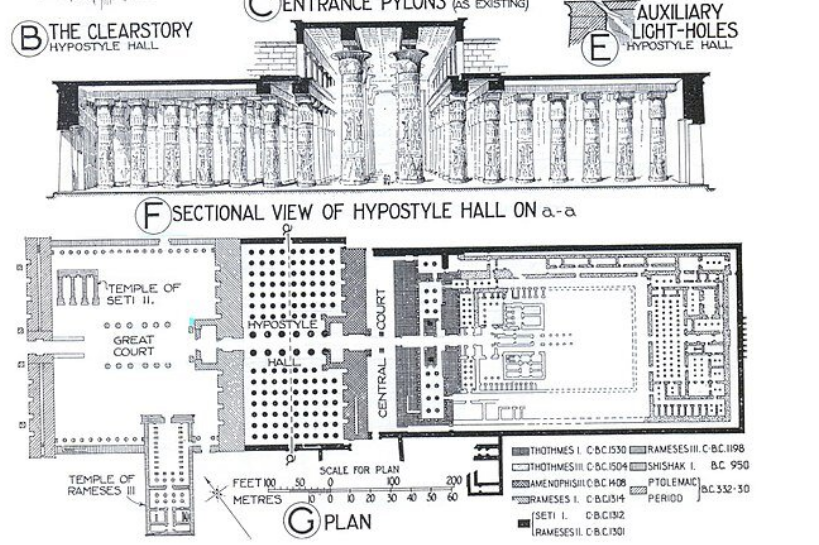
\includegraphics[width=14.5cm,height=8.6cm]{./figures/karnak.png}
\caption[Plan du Temple de Karnak]{\textit{Vue de la salle Hypostyle du Temple de Karnak en Haute Egypte} - Plan et coupe.} 
\label{fig:4:figure4}
\end{figure}

\begin{figure}
\centering
%%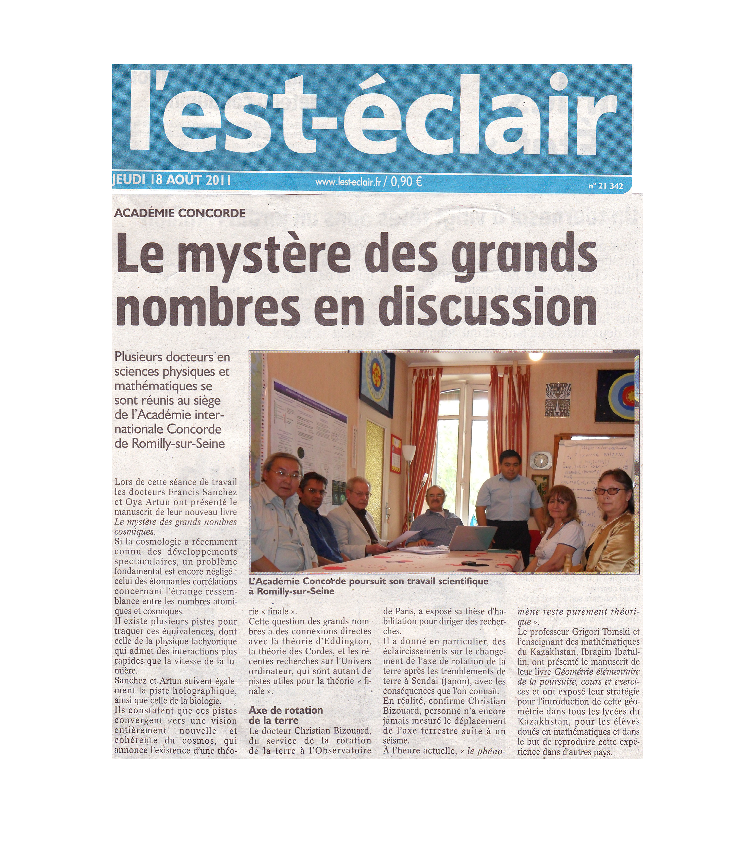
\includegraphics[width=13.5cm,height=11.0cm]{./figures/lesteclair.png}
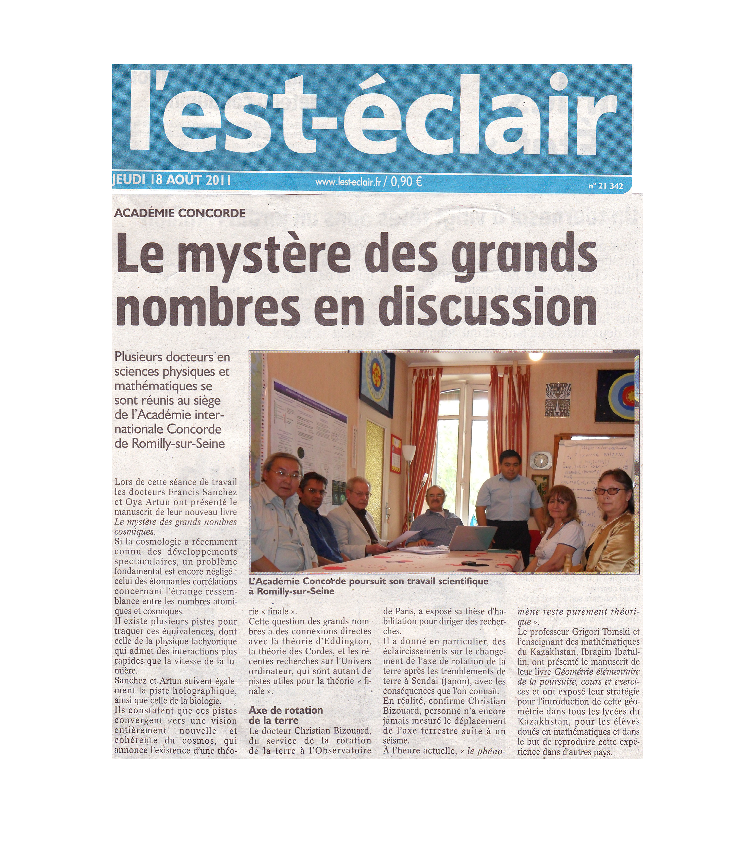
\includegraphics{./figures/lesteclair.png}
\caption [L'est-Eclair: Le mystere des grands nombres]{\textit{Le mystere des grands nombres} - Article du quotidien regional l'Est-Eclair du 18 Ao\^ut 2011.} 
\label{fig:5:figure5}
\end{figure}

\clearpage

\begin{figure}
\centering
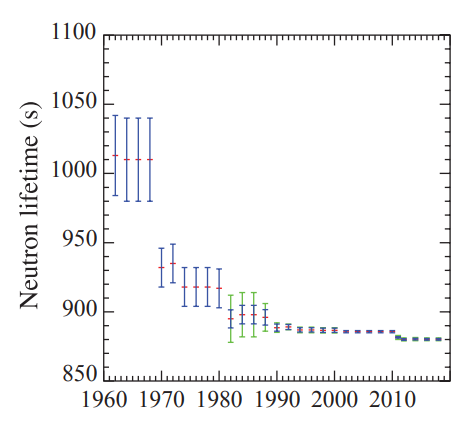
\includegraphics[width=8.5cm,height=4.5cm]{./figures/neutron-lifetime-pdg.png}
\caption[Mesures de la duree de vie du neutron depuis 1962]{\textit{Duree de vie du Neutron d'apres Particle Data Group 2019} - Tracé historique.} 
\label{fig:6:figure6}
\end{figure}

\begin{figure}
\centering
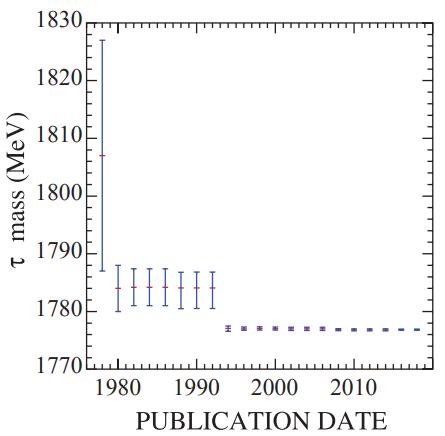
\includegraphics[width=8.5cm,height=4.5cm]{./figures/tau-mass-pdg.png}
\caption[Mesures de la masse du Tau depuis 1978]{\textit{Mesure de la masse du Tau d'apres Particle Data Group 2019} - Tracé historique.} 
\label{fig:7:figure7}
\end{figure}

\clearpage

\begin{figure}
\centering
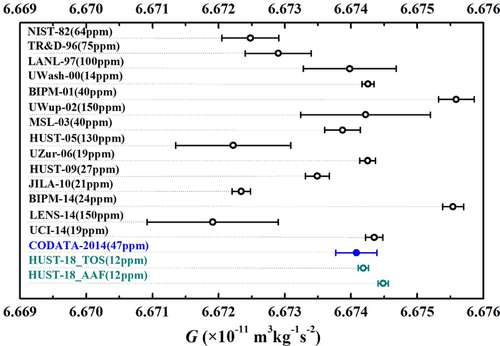
\includegraphics[width=8.5cm,height=4.5cm]{./figures/ProgressinPreciseMeasurementsoftheGravitationalConstant.png}
\caption[Mesures de la constante de gravitation G depuis 1982]{\textit{Mesures de la constante de gravitation G depuis 1982 d'apres Progress in Precise Measurements of the Gravitational Constant \cite{Wu}} - Tracé historique.} 
\label{fig:8:figure8}
\end{figure}

\clearpage

\begin{figure}
\centering
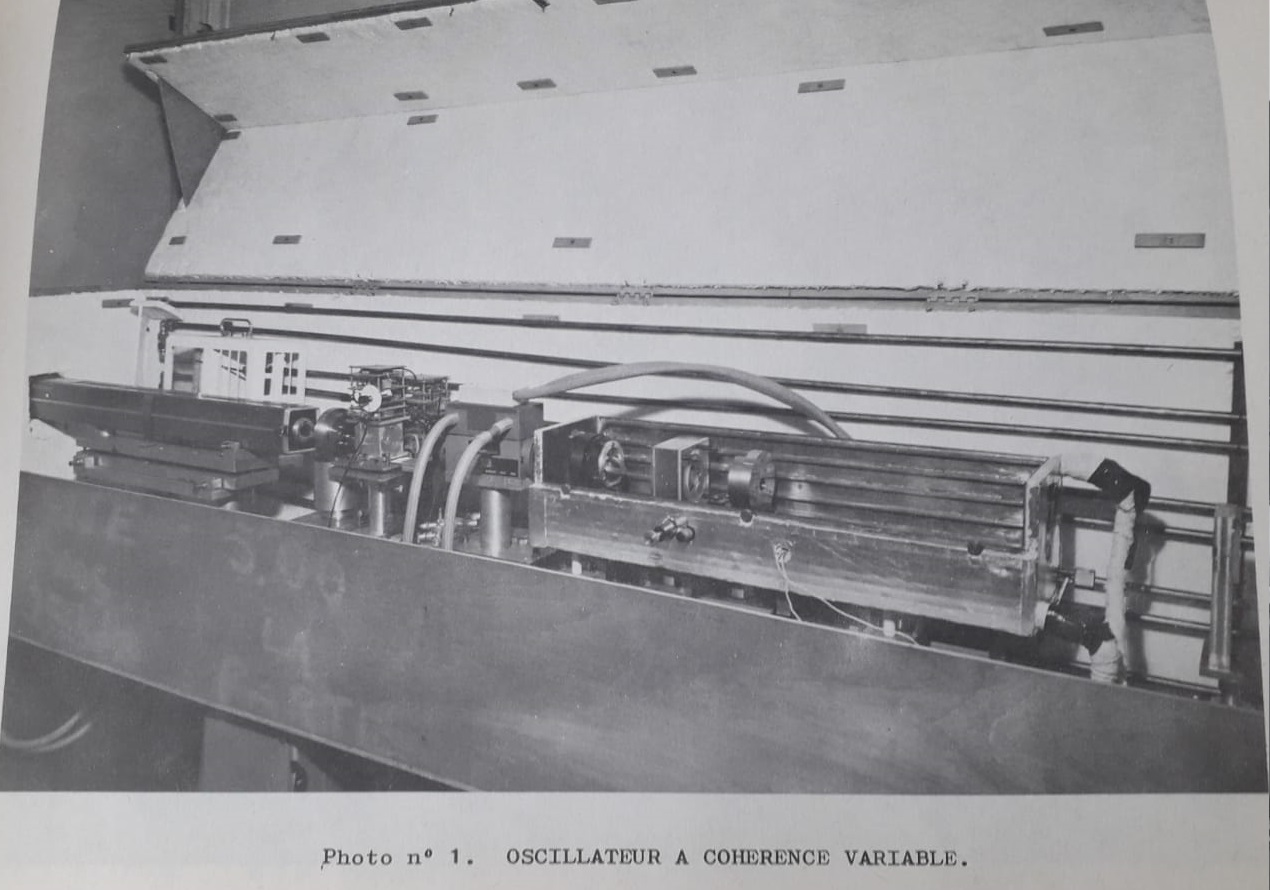
\includegraphics[width=14.5cm,height=8.6cm]{./figures/oscillateur-CEA-multiphotonGroup.jpg}
\caption[Vue de l'oscillateur du LASER $Nd^{3p+}$]{\textit{Oscillateur du LASER $Nd^{3p+}$ } - Photo realise au CEA en 1973.} 
\label{fig:9:figure9}
\end{figure}

\begin{figure}
\centering
%%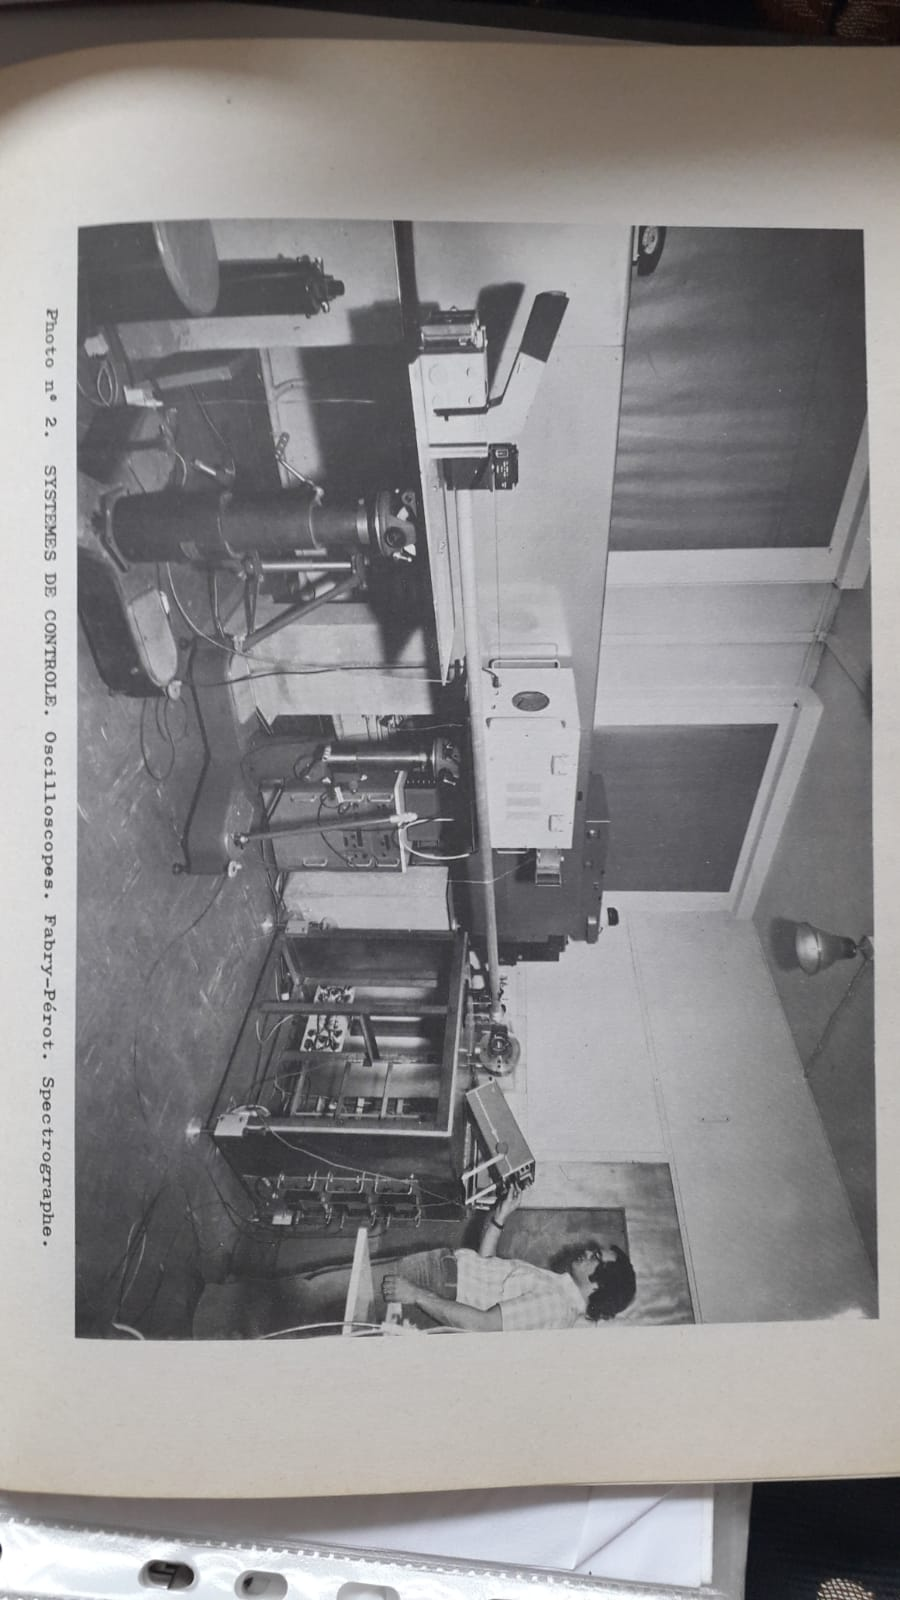
\includegraphics[width=14.5cm,height=8.6cm]{./figures/ControlSystemOscilloFabryPerot-CEA-multiphotonGroup.jpg}
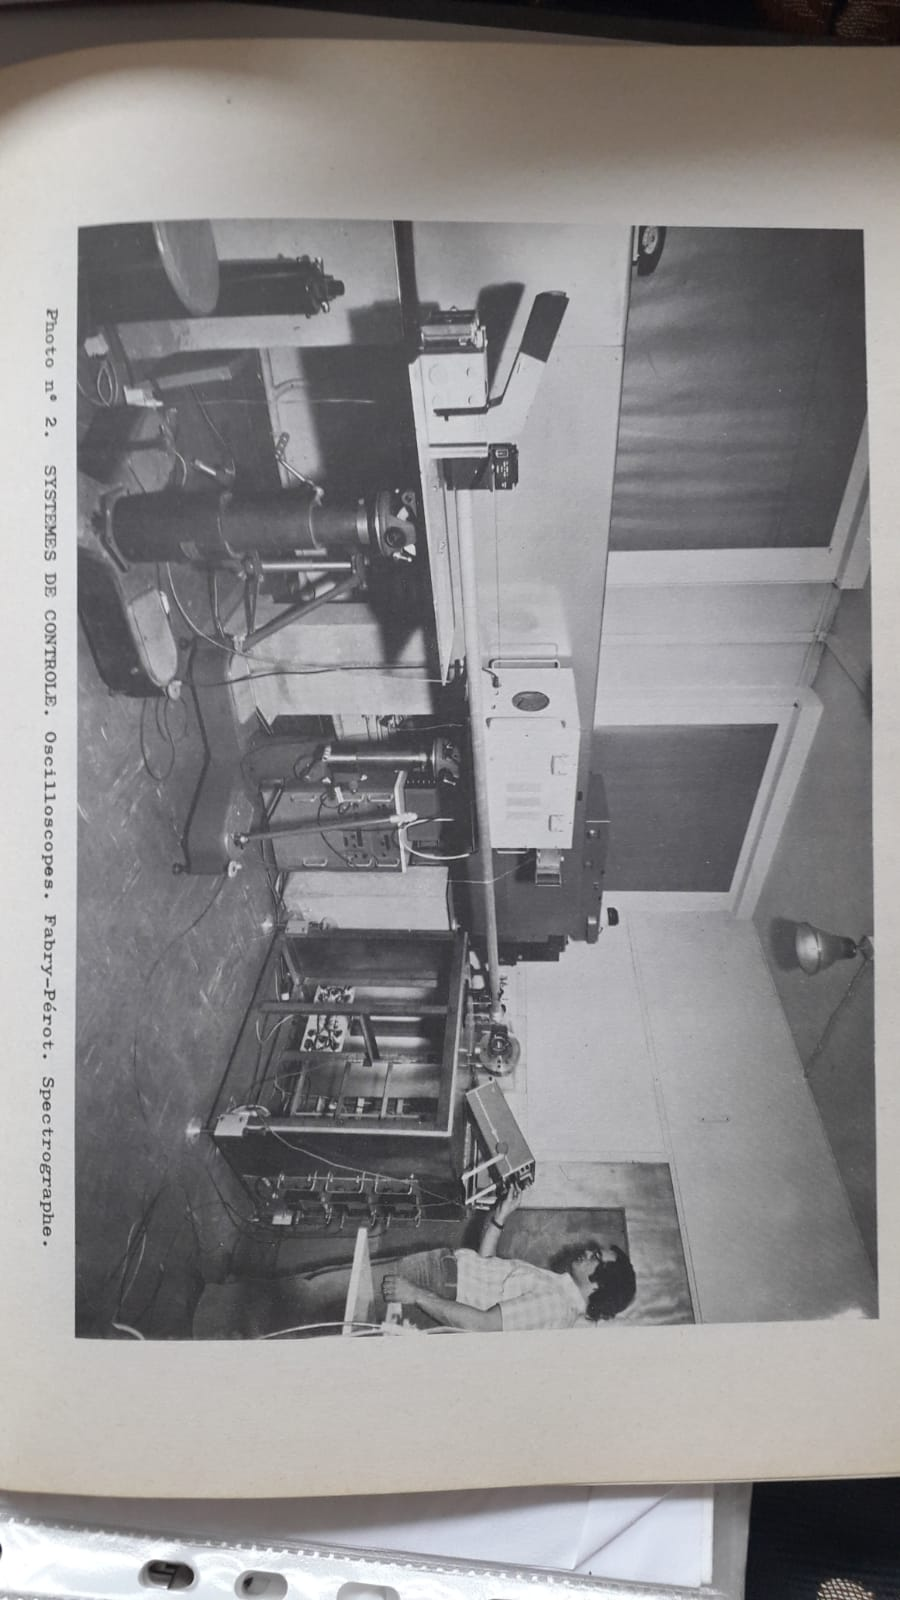
\includegraphics[width=14.5cm,height=8.6cm]{./figures/ControlSystemOscilloFabryPerot-CEA-multiphotonGroup.jpg}
\caption[Vue du systeme de controle du LASER $Nd^{3p+}$]{\textit{Systeme de controle du LASER $Nd^{3p+}$ muni d'oscilloscope, de spectrographe et de cavite Fabry-Perot} - Photo realisé au CEA en 1973.} 
\label{fig:10:figure10}
\end{figure}

\clearpage

\begin{figure}
\centering
\includegraphics[width=12.5cm,height=7.5cm]{./figures/Cambridge.jpg}
\caption[La conference de l'ANPA a Cambridge en 1995]{\textit{La conference de l'ANPA a Cambridge: 2eme rang assis de droite a gauche: Mike Manthey, Clive Kilmister, Francis Sanchez, ... debout: K. Bowden, Geoffrey Constable, Peter Marcer, ..., ..., P. Noyes} Sept 1995 }
\label{fig:11:figure11}
\end{figure}


\begin{figure}
\centering
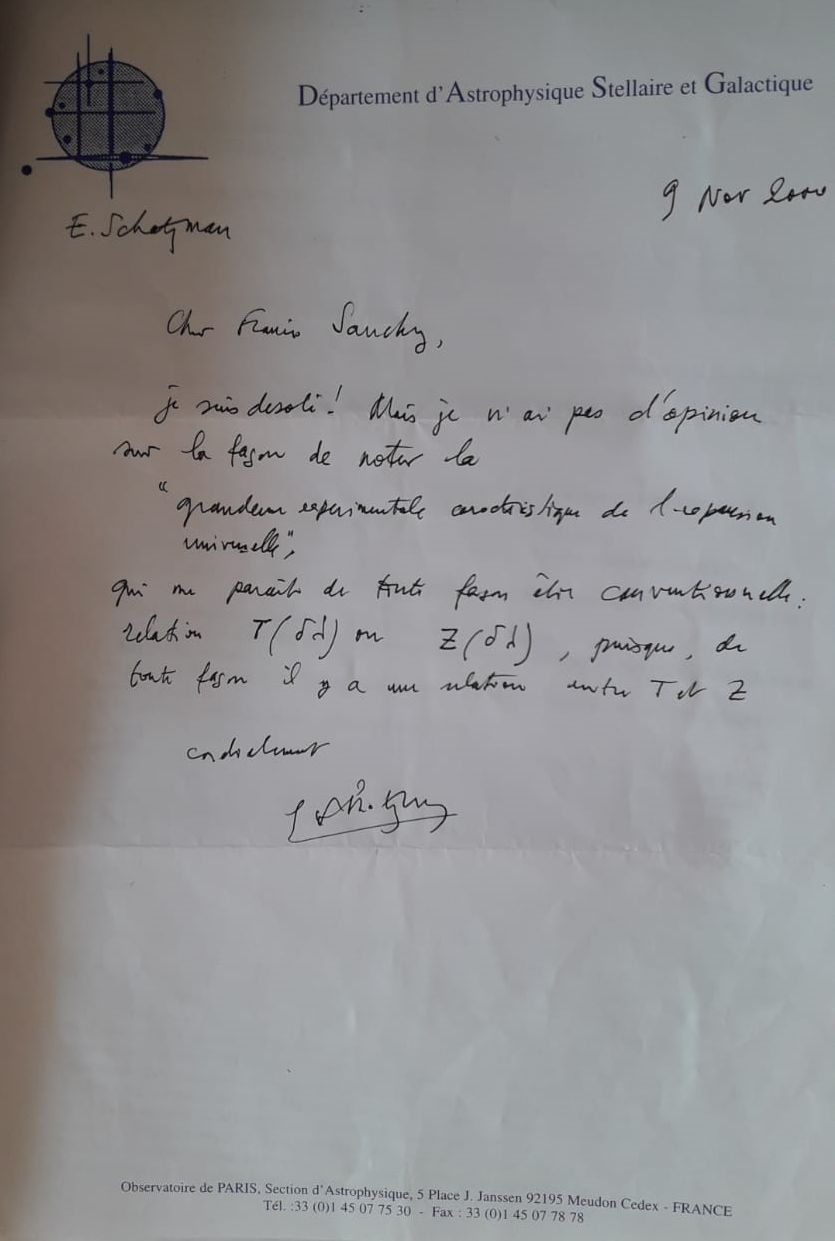
\includegraphics[width=8.5cm,height=14.5cm]{./figures/schatzmann.png}
\caption[Courrier d evaluation d E.Schatzman]{\textit{Courrier de E.Schatzman du Département d'Astrophysique Stellaire et Galactique évaluant le rapport sur la cosmologie de Francis M. Sanchez} - 9 Nov 2000.} 
\label{fig:12:figure12}
\end{figure}


\begin{figure}
\centering
%%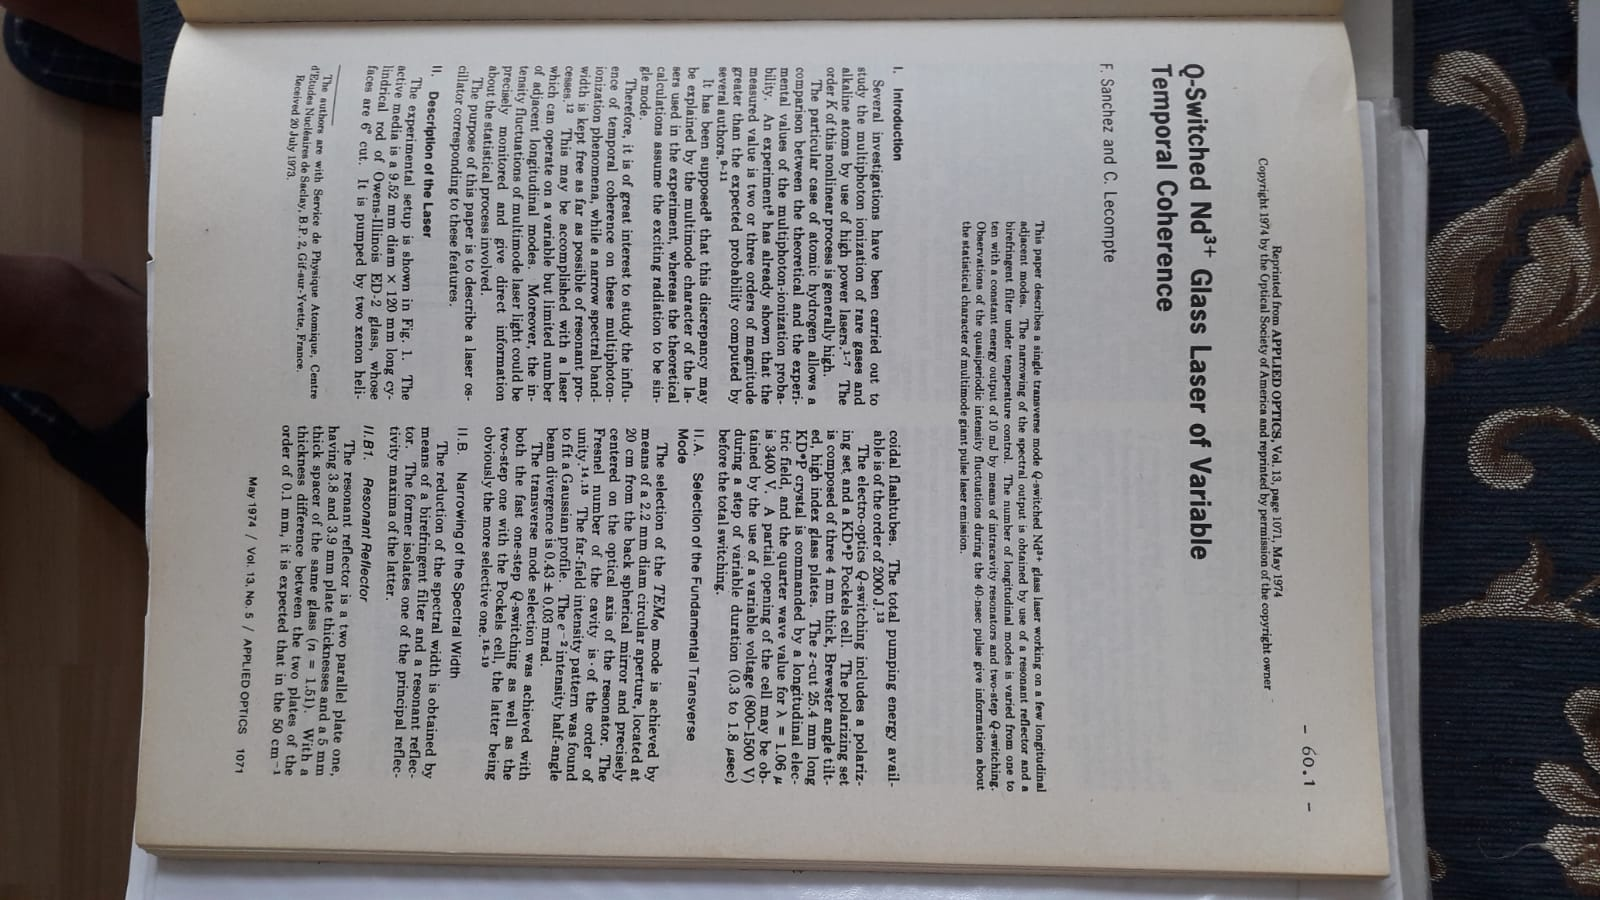
\includegraphics[width=14.5cm,height=8.6cm]{./figures/Nd3PlusGlassLASER-paper-1973.jpg}
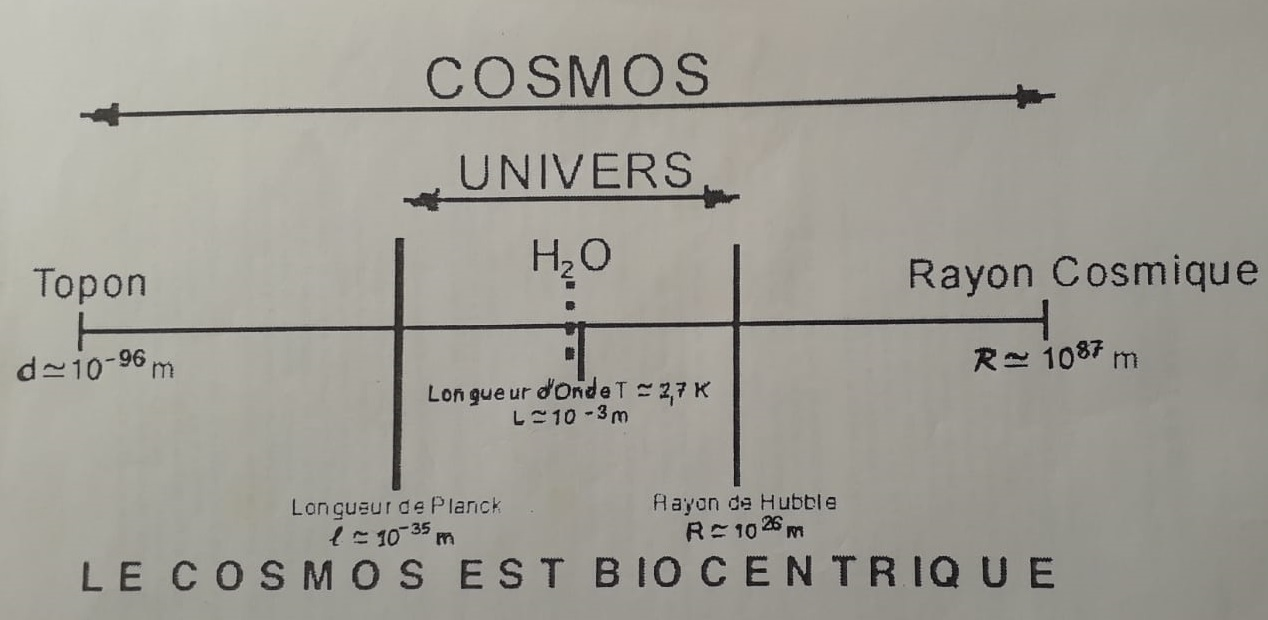
\includegraphics[width=14.5cm,height=8.5cm]{./figures/h2o-biocentrique.jpg}
\caption[Schema du Cosmos Biocentrique $H_2O$ ]{\textit{Schema du cosmos biocentrique autour de $H_2O$} - 9 Nov 2000.} 
\label{fig:13:figure13}
\end{figure}

\begin{figure}
\centering
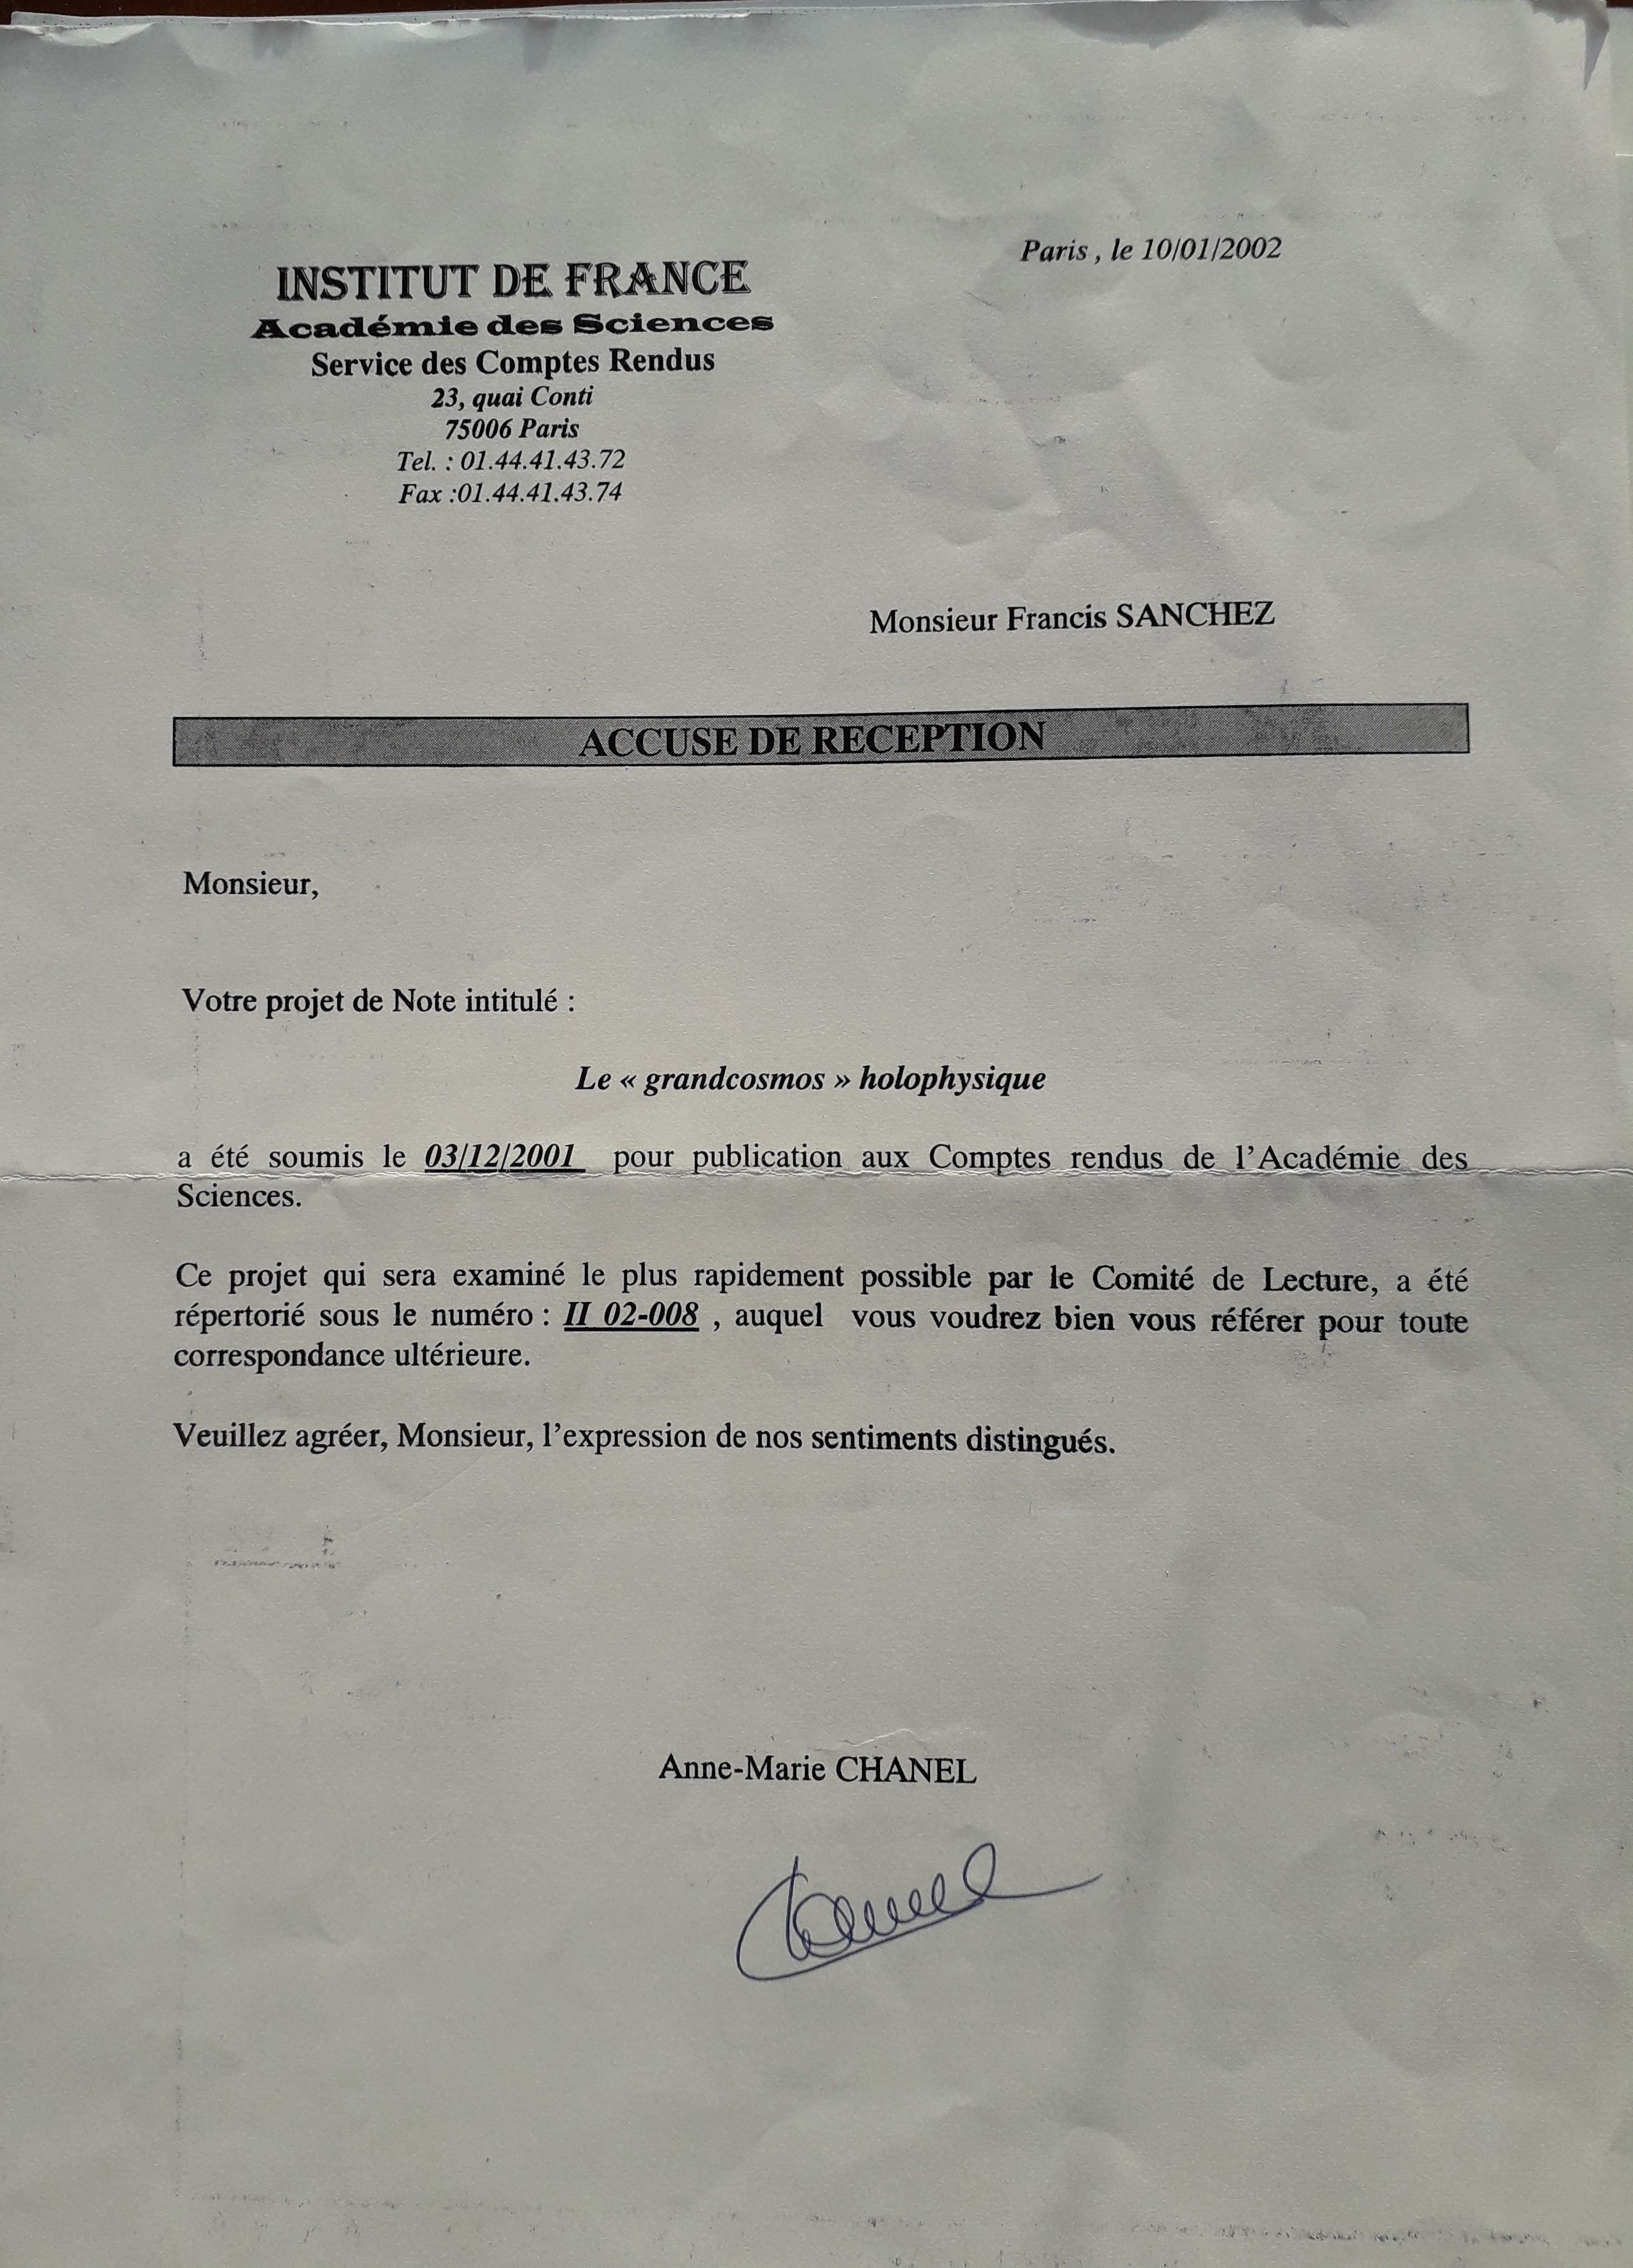
\includegraphics[width=8.5cm,height=14.5cm]{./figures/AcadSciences2001.jpg}
\caption[Accuse reception du depot du compte-rendu aupres de l'Academie des Sciences]{\textit{Accuse reception du compte-rendu intitulé ``Le Grandcosmos Holophysique'' déposé aupres de l'Académie des Sciences par l'intermédiaire de l'institut de France} - 03 DEC 2001.} 
\label{fig:14:figure14}
\end{figure}

\begin{figure}
\centering
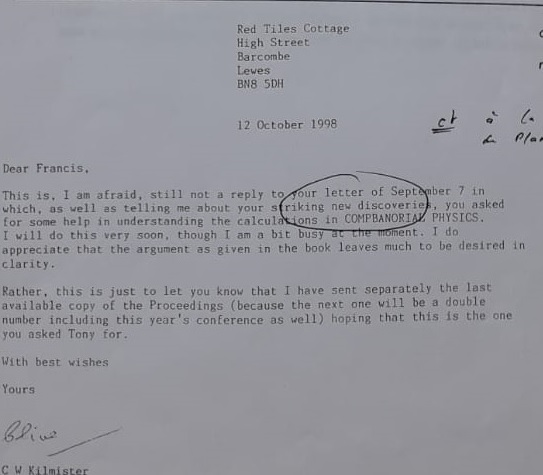
\includegraphics[width=8.5cm,height=14.5cm]{./figures/kilmister.jpg}
\caption[Rapport de Kilmister]{\textit{Rapport de Clive Kilmister} -  1998.} 
\label{fig:15:figure15}
\end{figure}

\begin{figure}
\centering
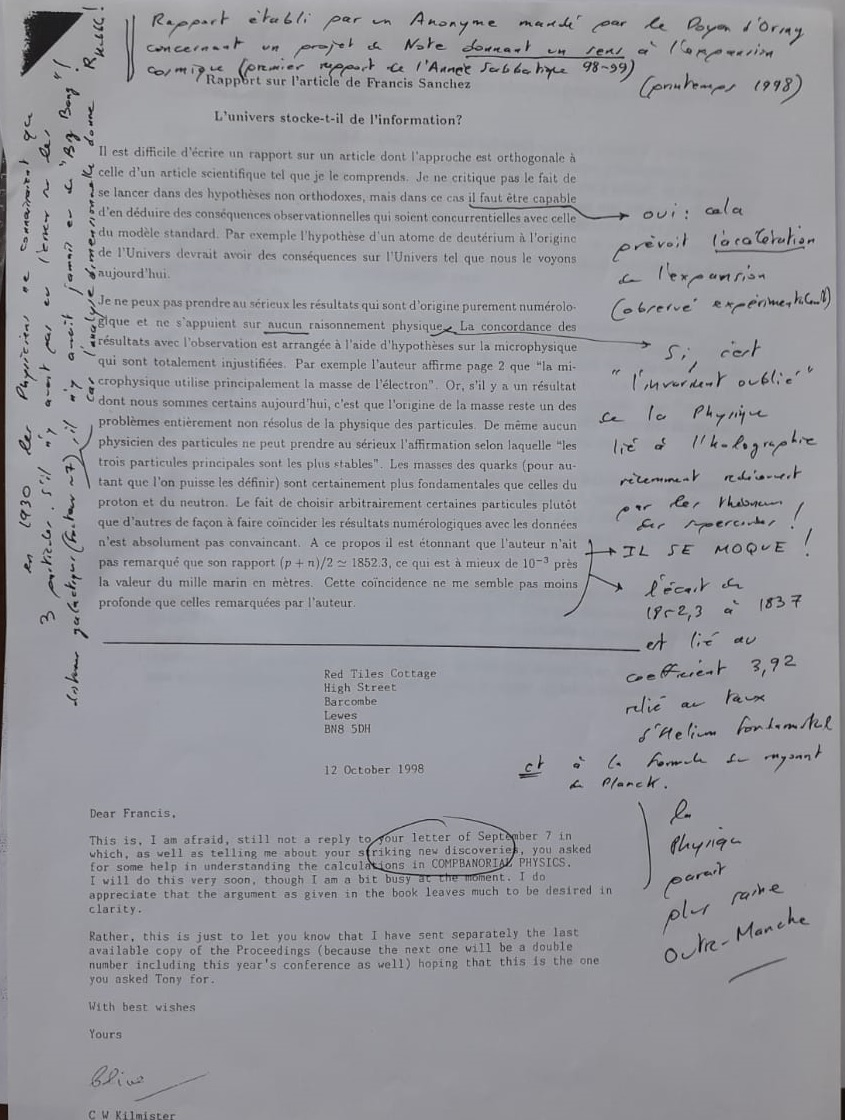
\includegraphics[width=8.5cm,height=14.5cm]{./figures/rapportAnonyme.jpg}
\caption[Rapport Anonyme demande par le doyen de l'universite d'Orsay]{\textit{Rapport anonyme sur ``L'univers stocke-t-il de l'information ?''} -  1998.} 
\label{fig:16:figure16}
\end{figure}

\begin{figure}
\centering
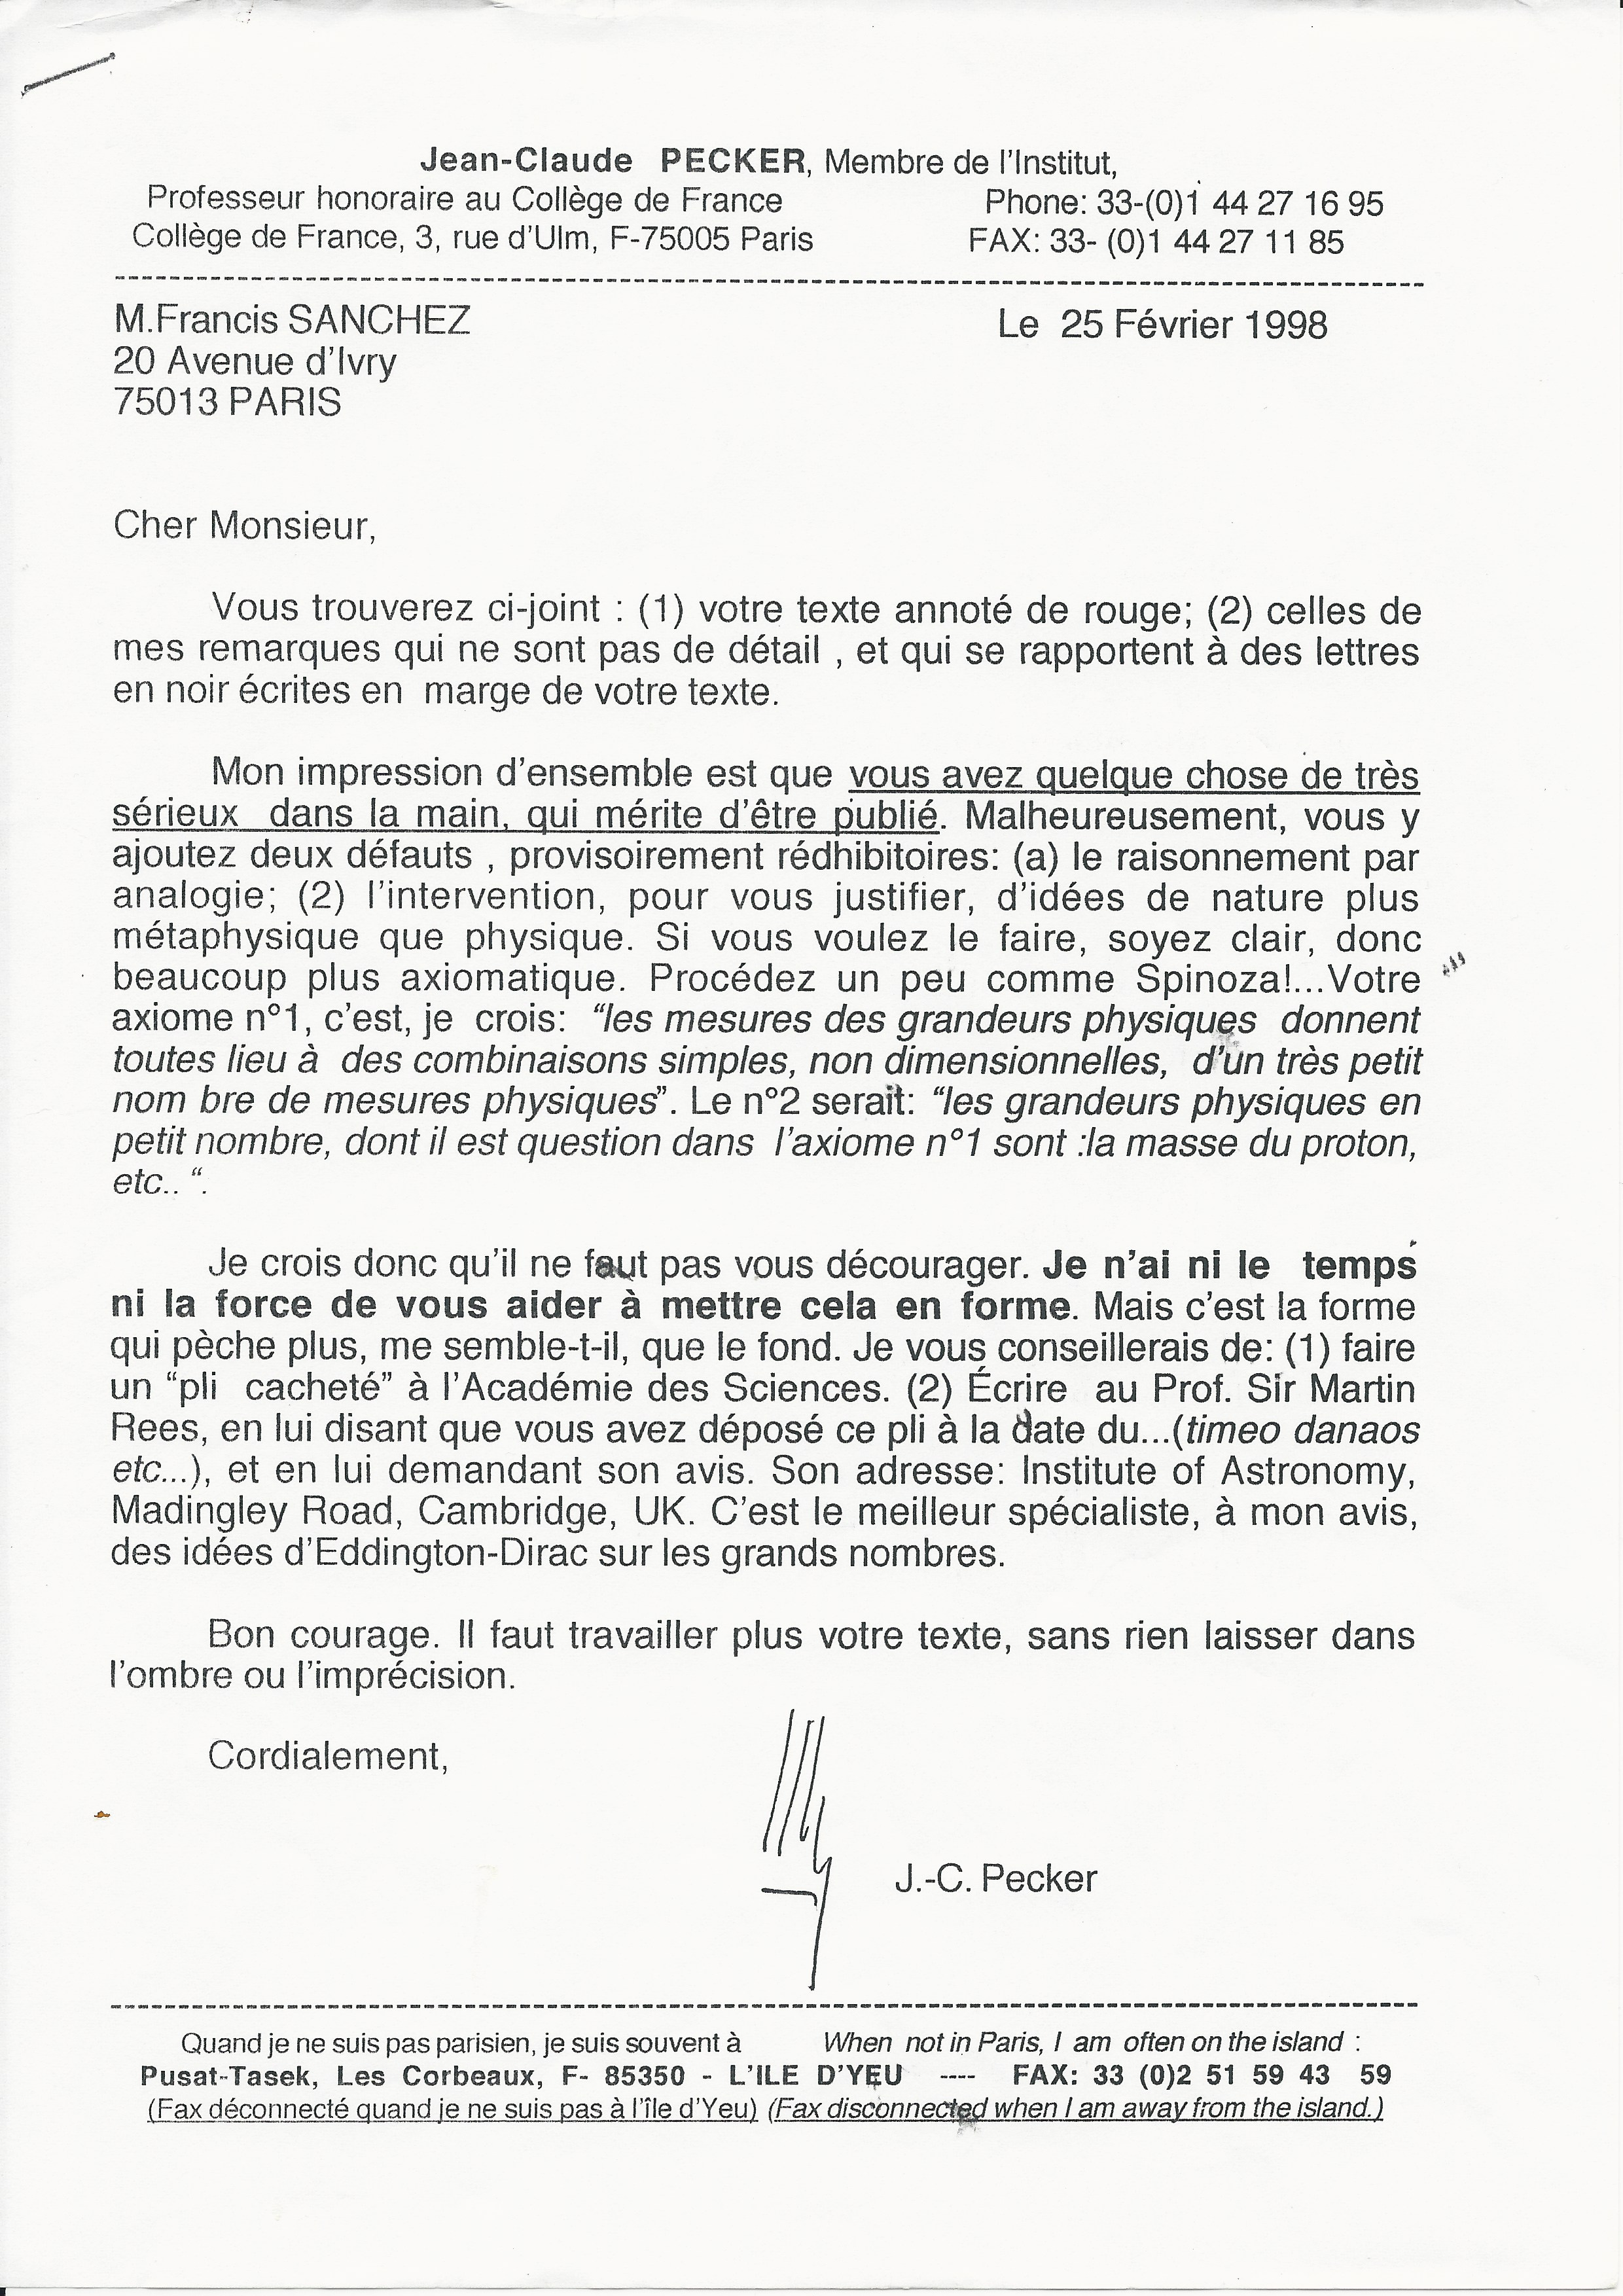
\includegraphics[width=8.5cm,height=11.5cm]{./figures/Pecker98.jpg}
%%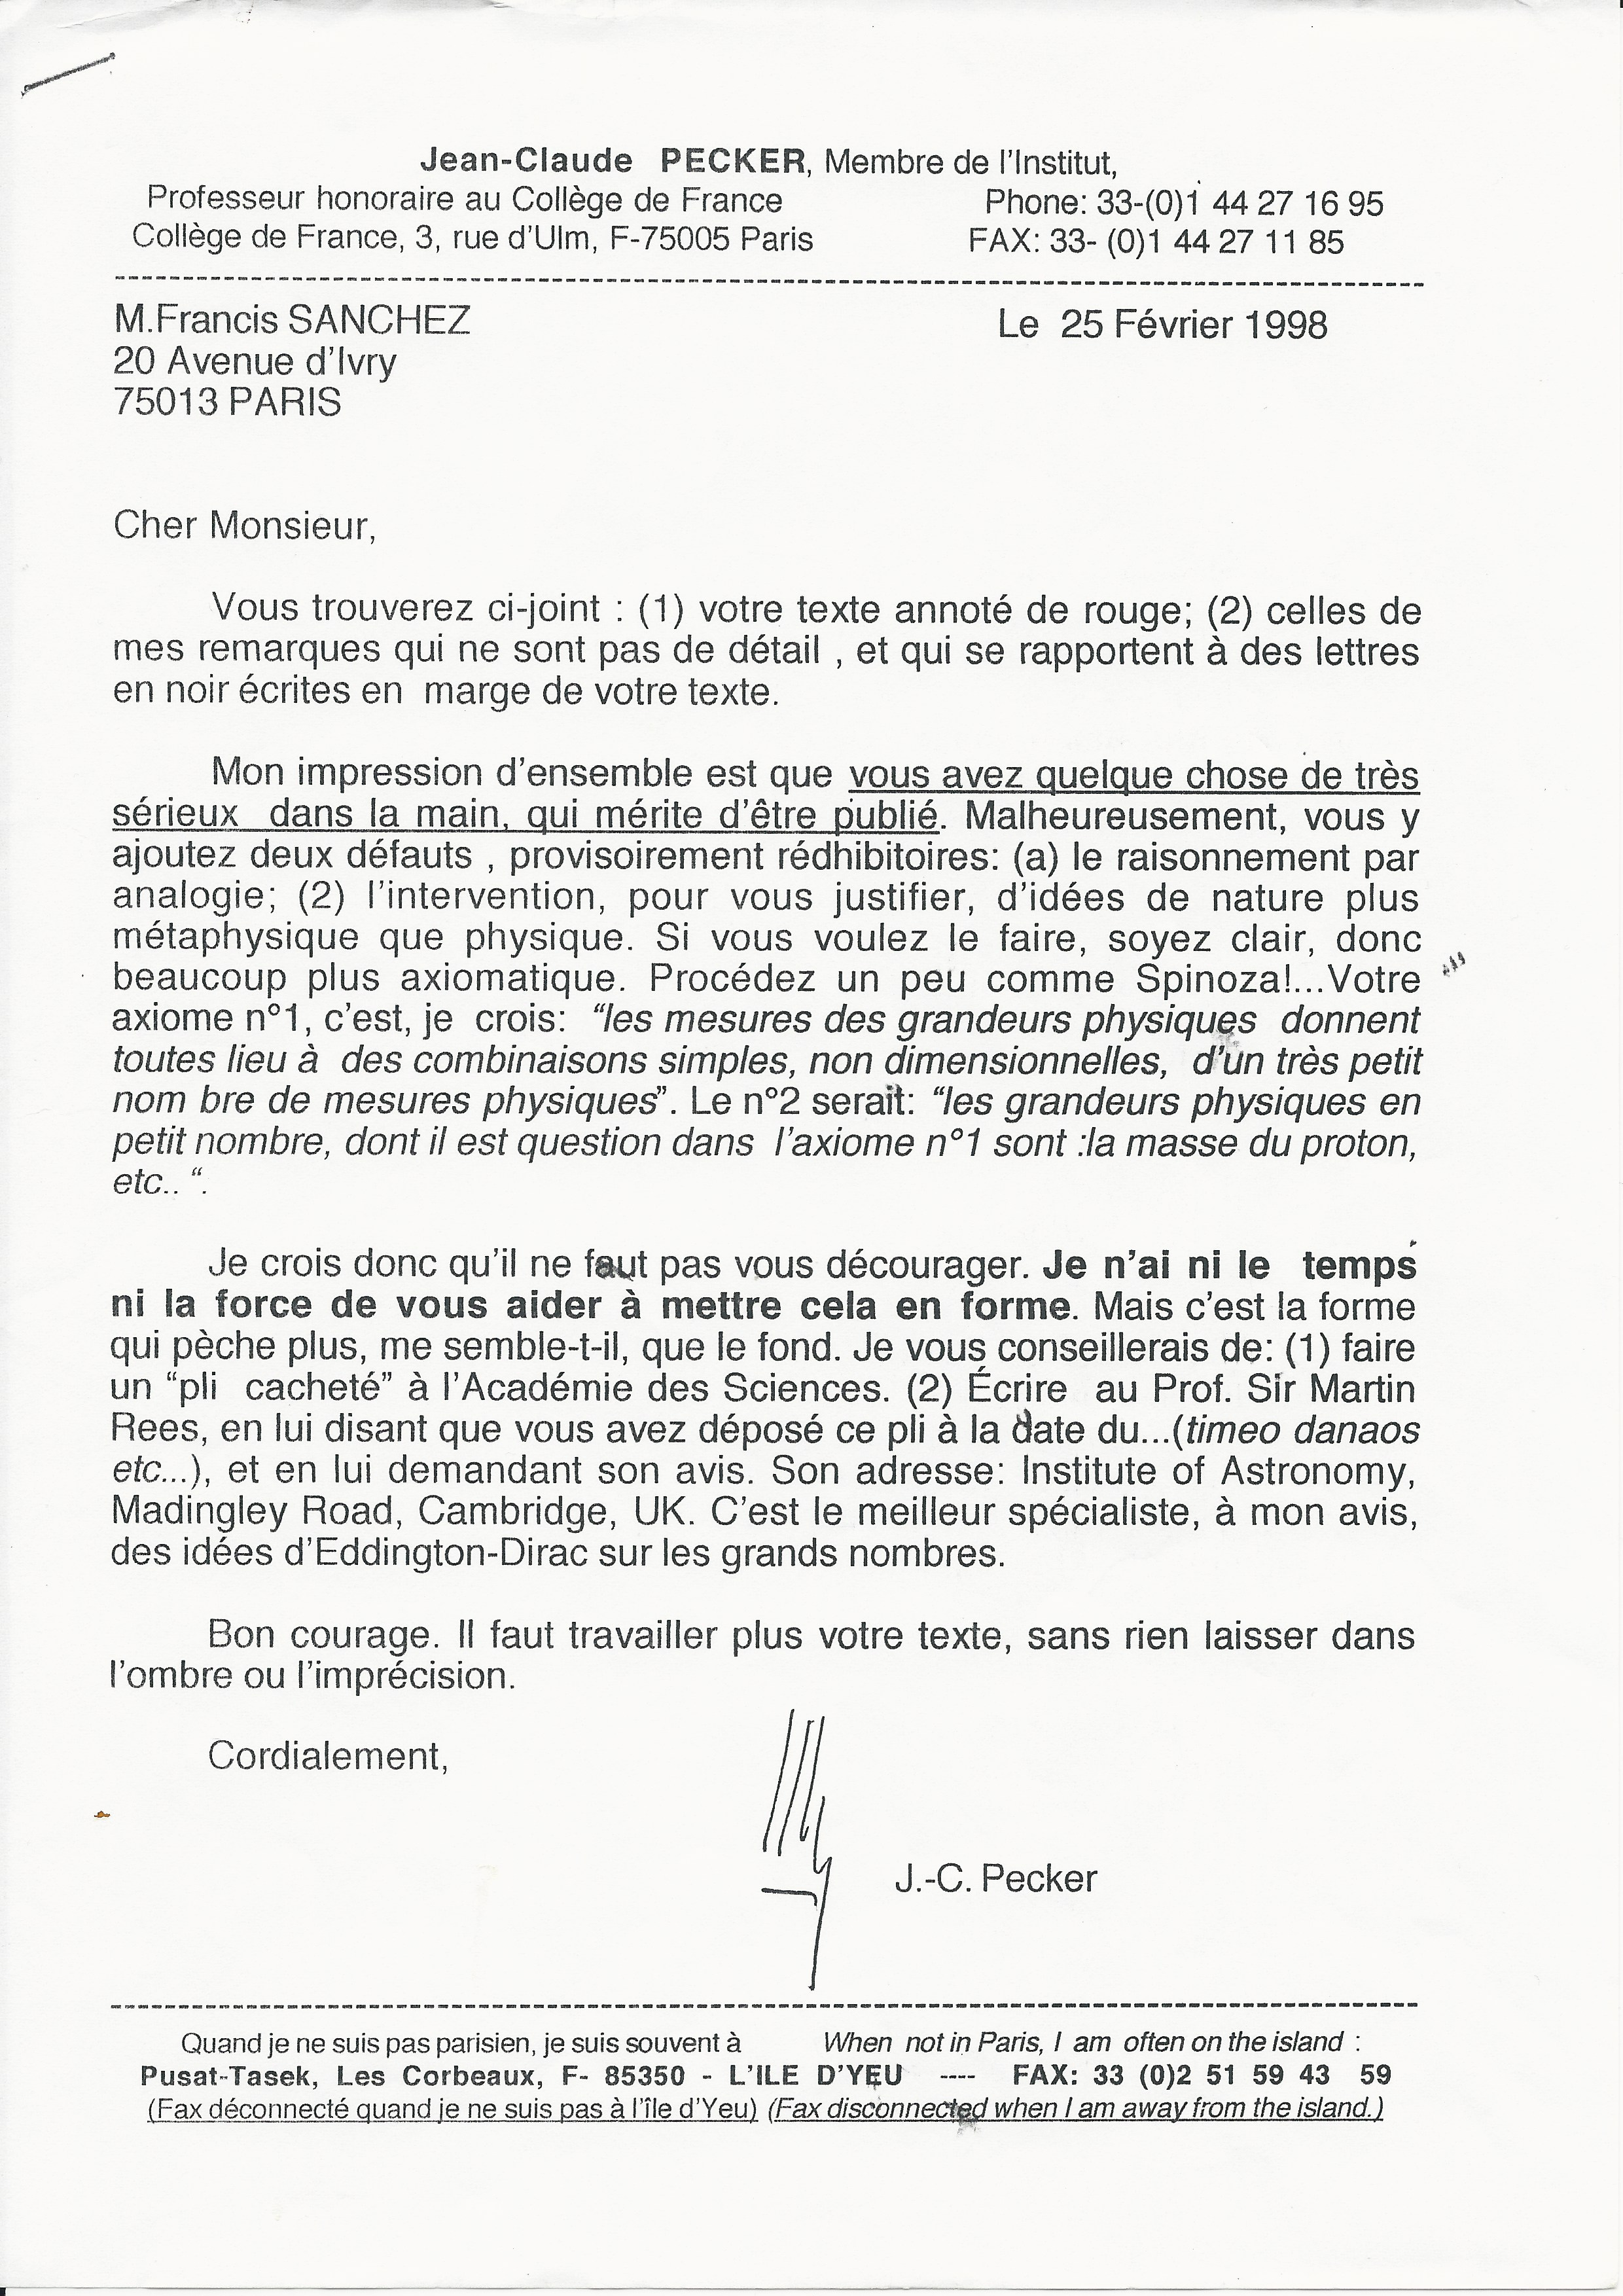
\includegraphics{./figures/Pecker98.jpg}
\caption[Rapport de JC Pecker sur la theorie de Francis M. Sanchez]{\textit{Rapport de J-C Pecker membre de l'Institut professeur honoraire au college de France} - 25 Fev 1998.} 
\label{fig:17:figure17}
\end{figure}


\begin{figure}
\centering
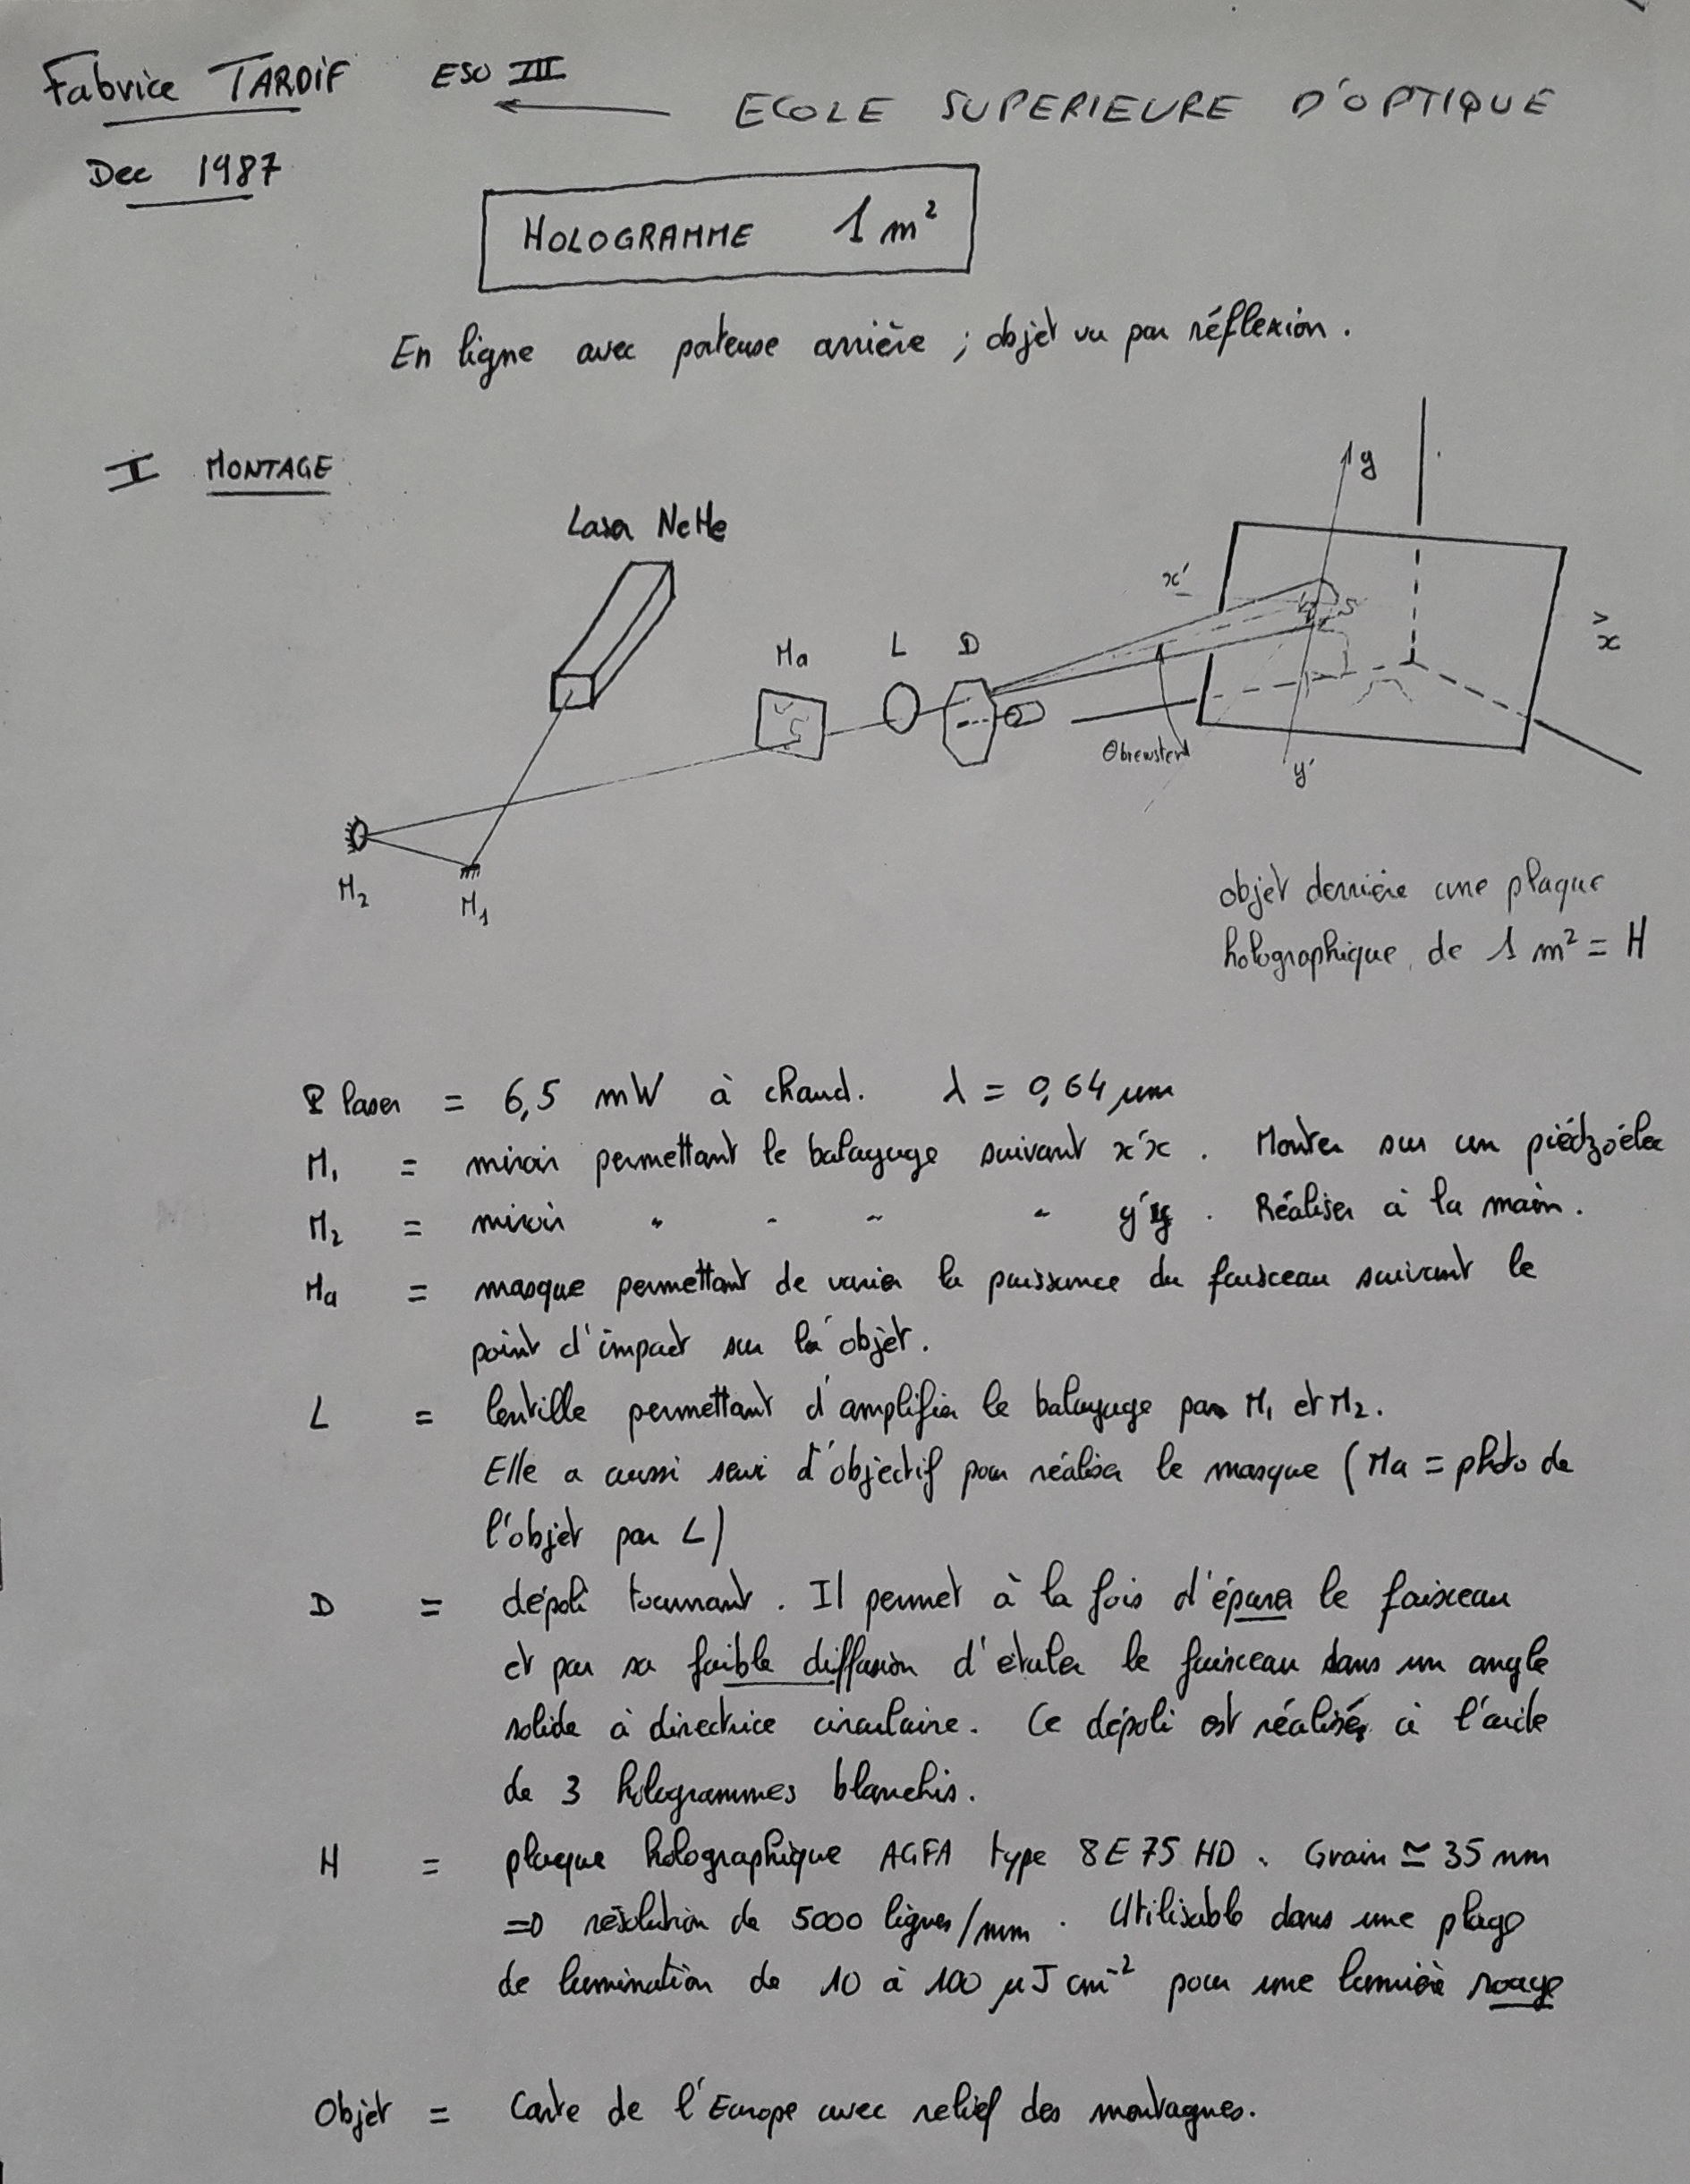
\includegraphics[width=8.5cm,height=11.5cm]{./figures/Tardif1987.png}
\caption[Rapport de Fabrice Tardif sur l'holographie a balayage]{\textit{Rapport de Fabrice Tardif sur l'holographie à balayage} décembre 1987}
\label{fig:18:figure18}
\end{figure}

\clearpage

\begin{figure}
\centering
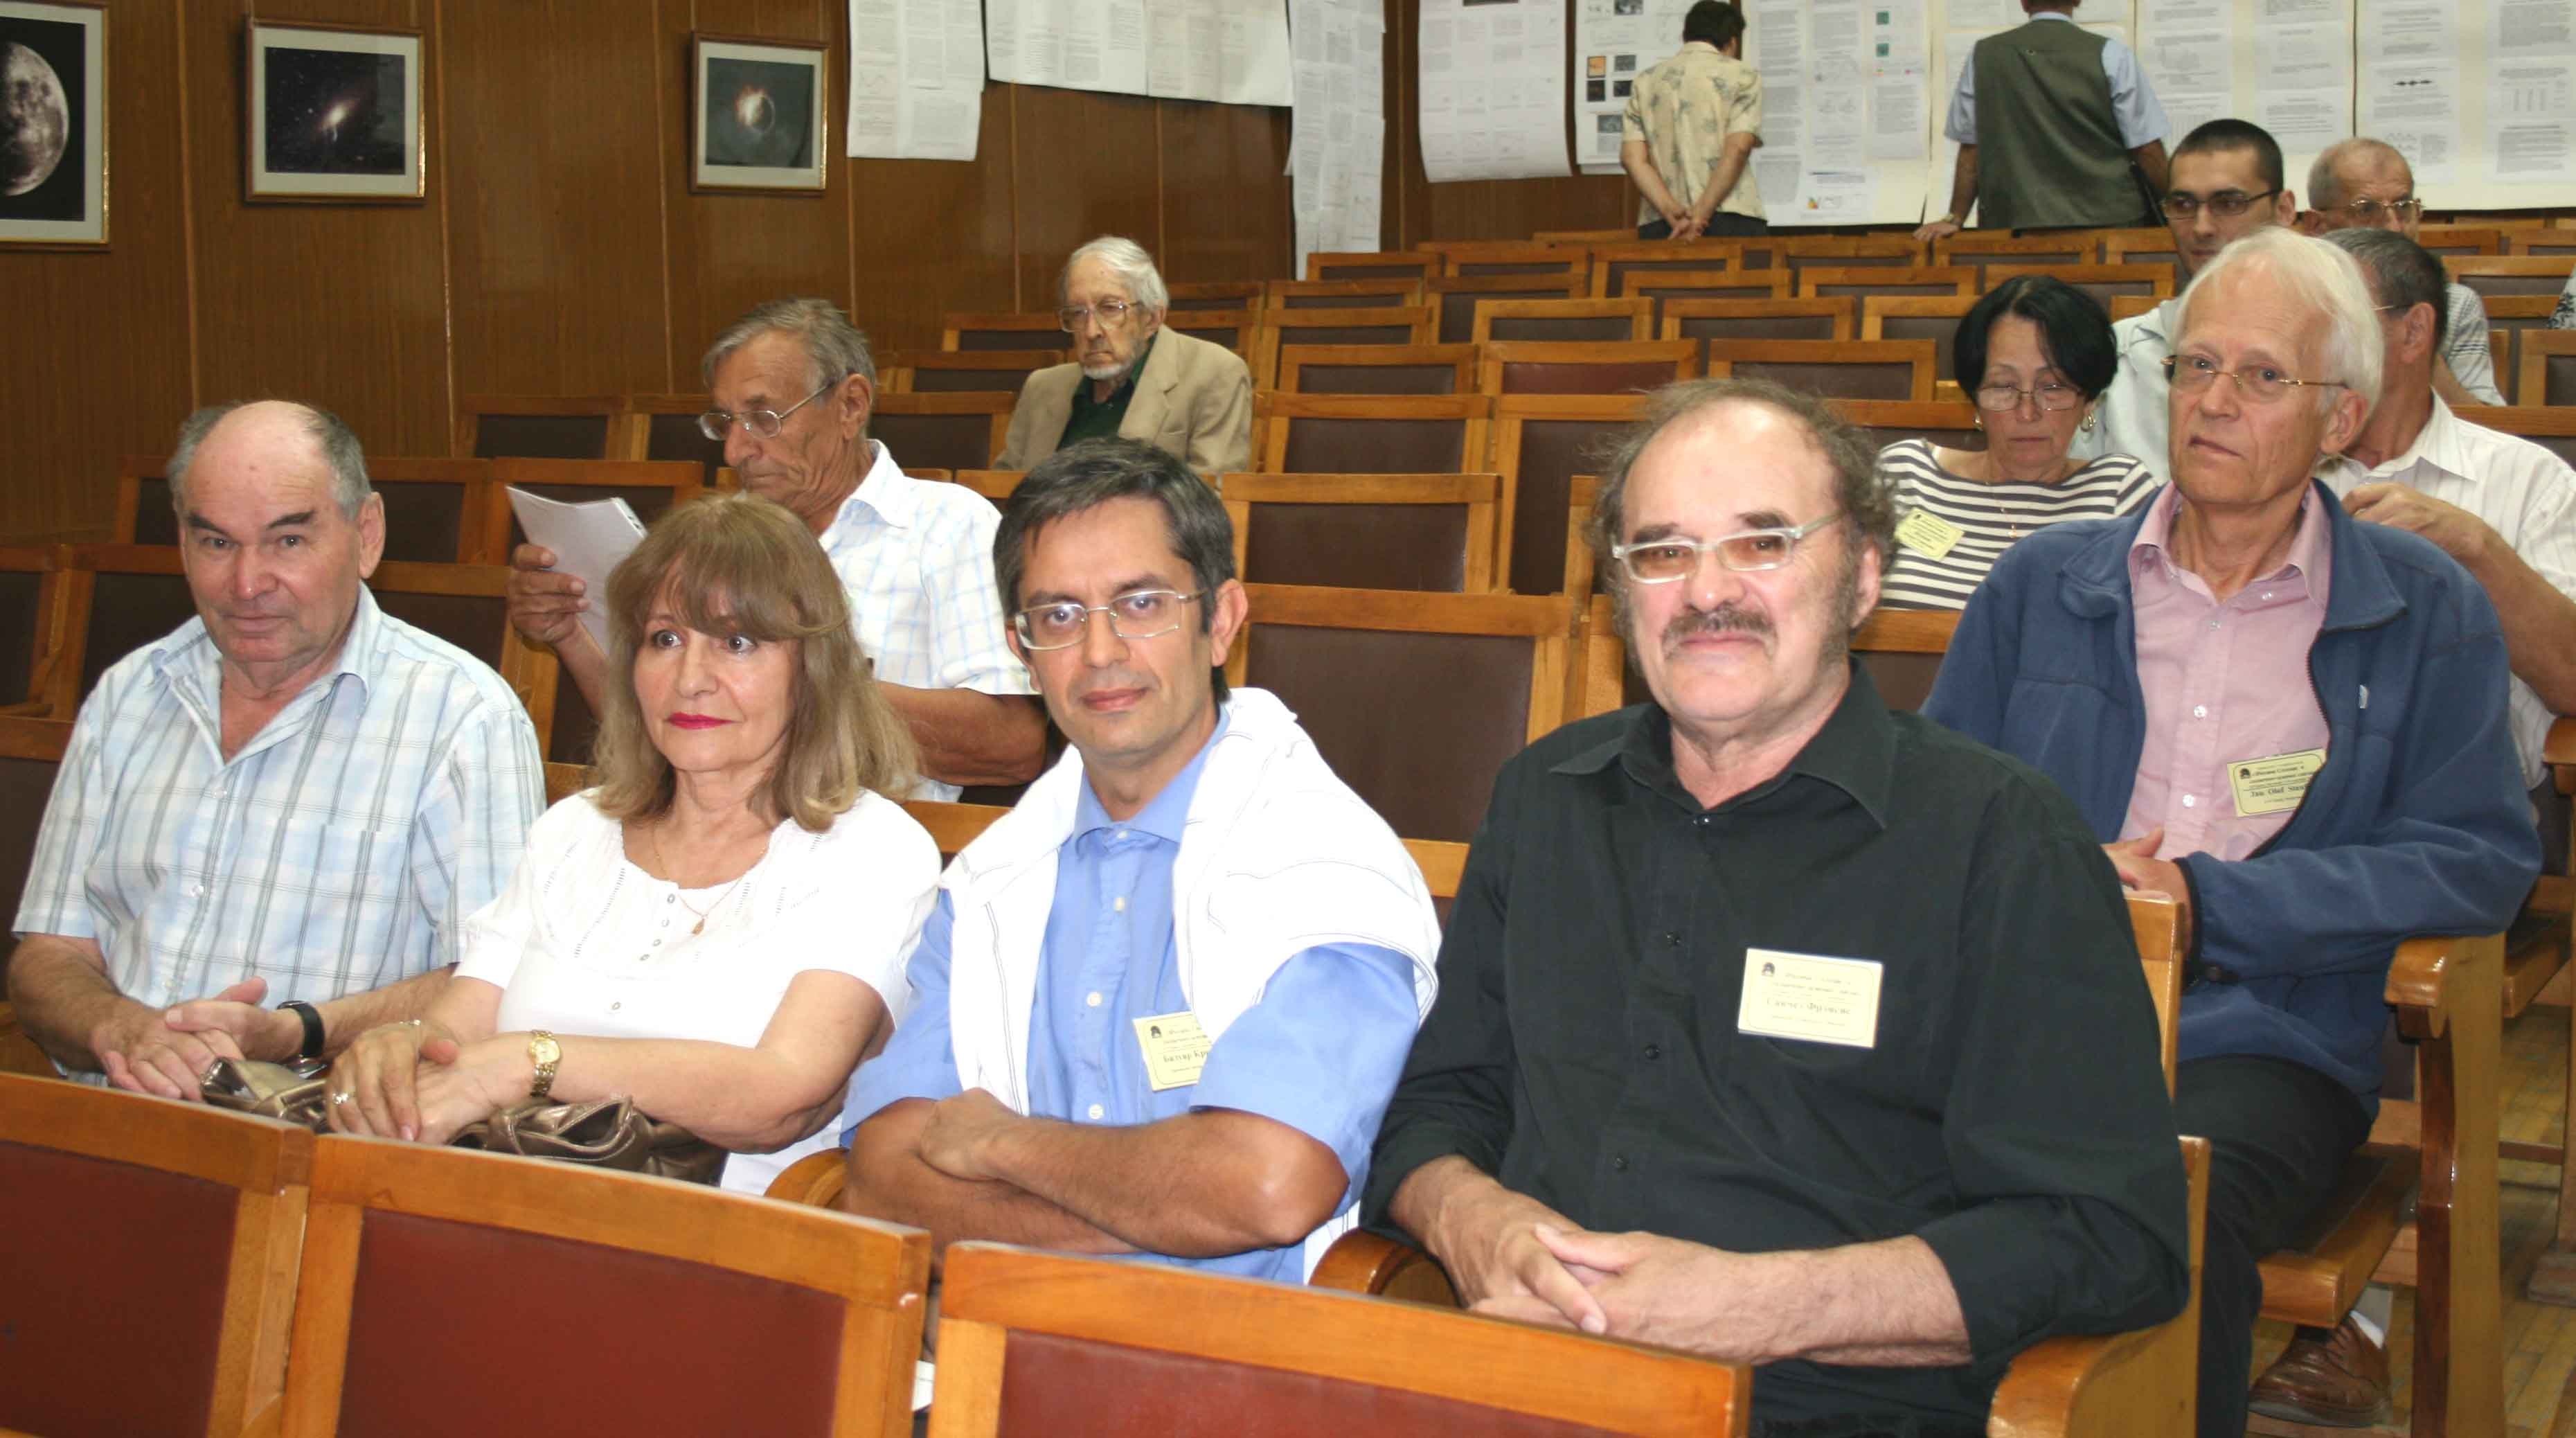
\includegraphics[width=12.5cm,height=7.5cm]{./figures/Kotov.jpg}
%%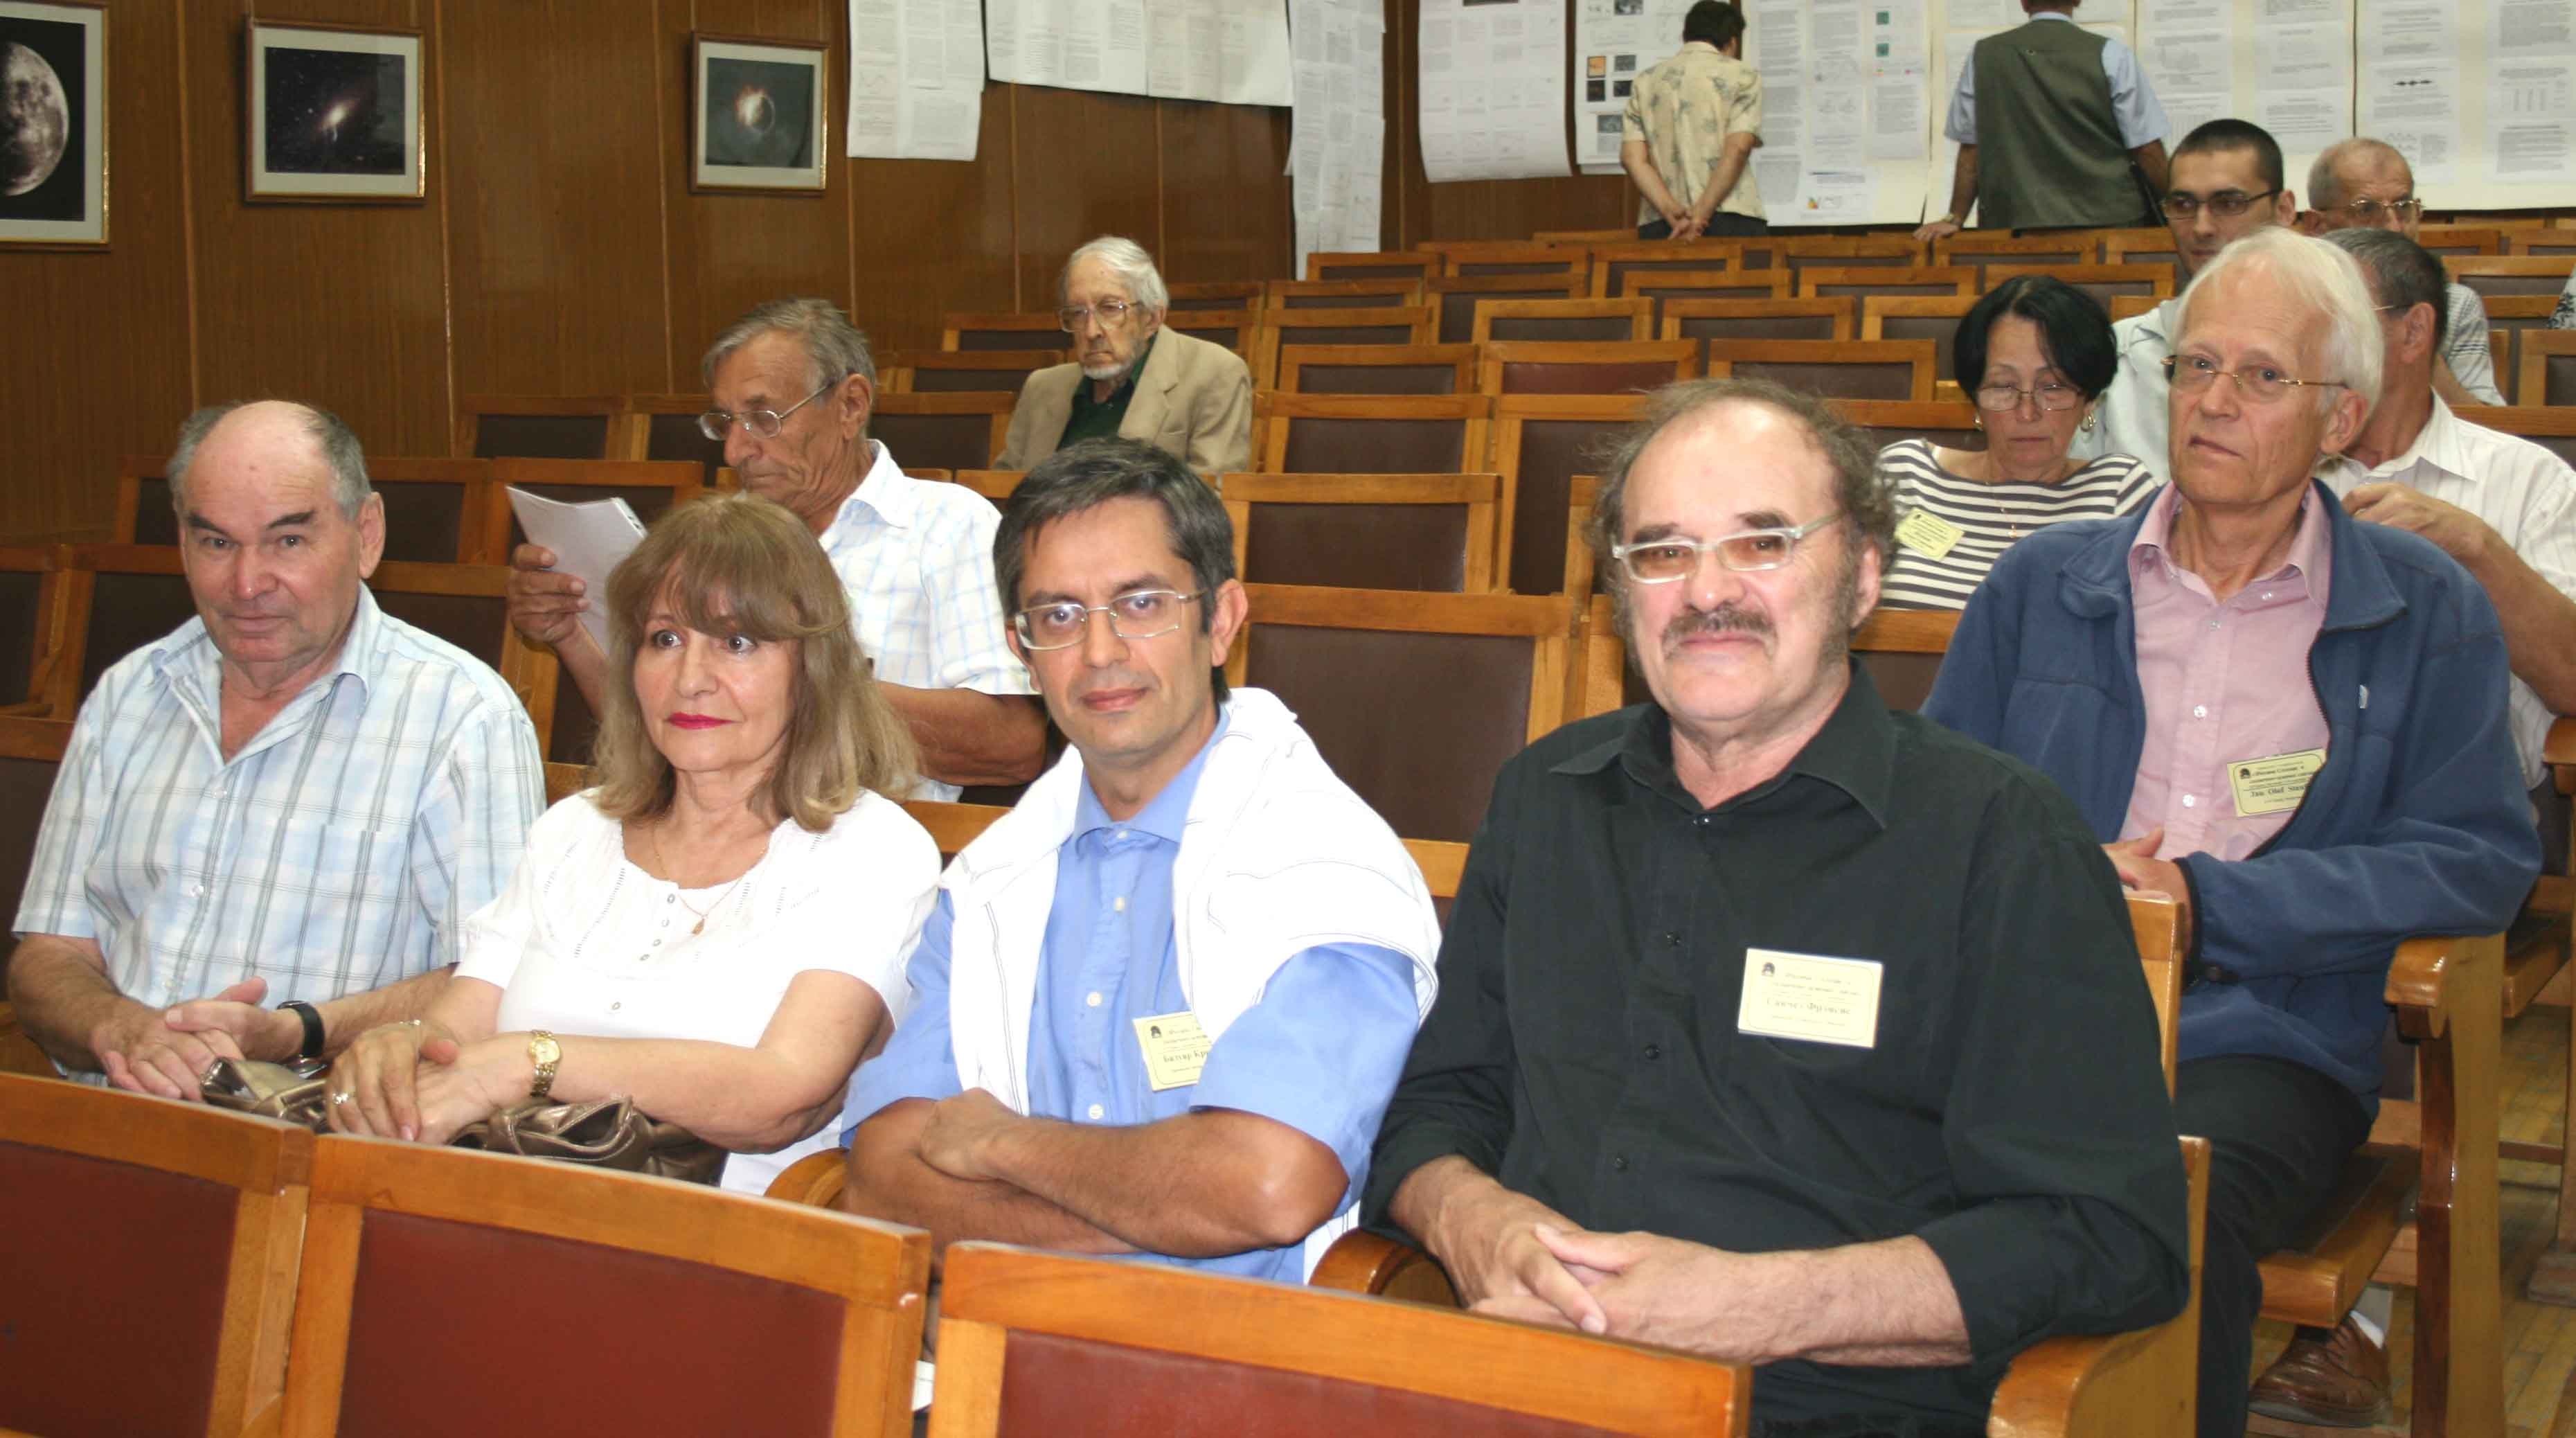
\includegraphics{./figures/Kotov.jpg}
\caption[Reunion a l'observatoire de Crimee]{\textit{La réunion à l'observatoire de Crimée: 1er rang de droite a gauche: Francis Sanchez, Christian Bizouard, Oya Artun, Valery Kotov. 2eme rang à droite Jan  directeur de l'Observatoire de } 2008}
\label{fig:19:figure19}
\end{figure}

\clearpage

\begin{figure}
\centering
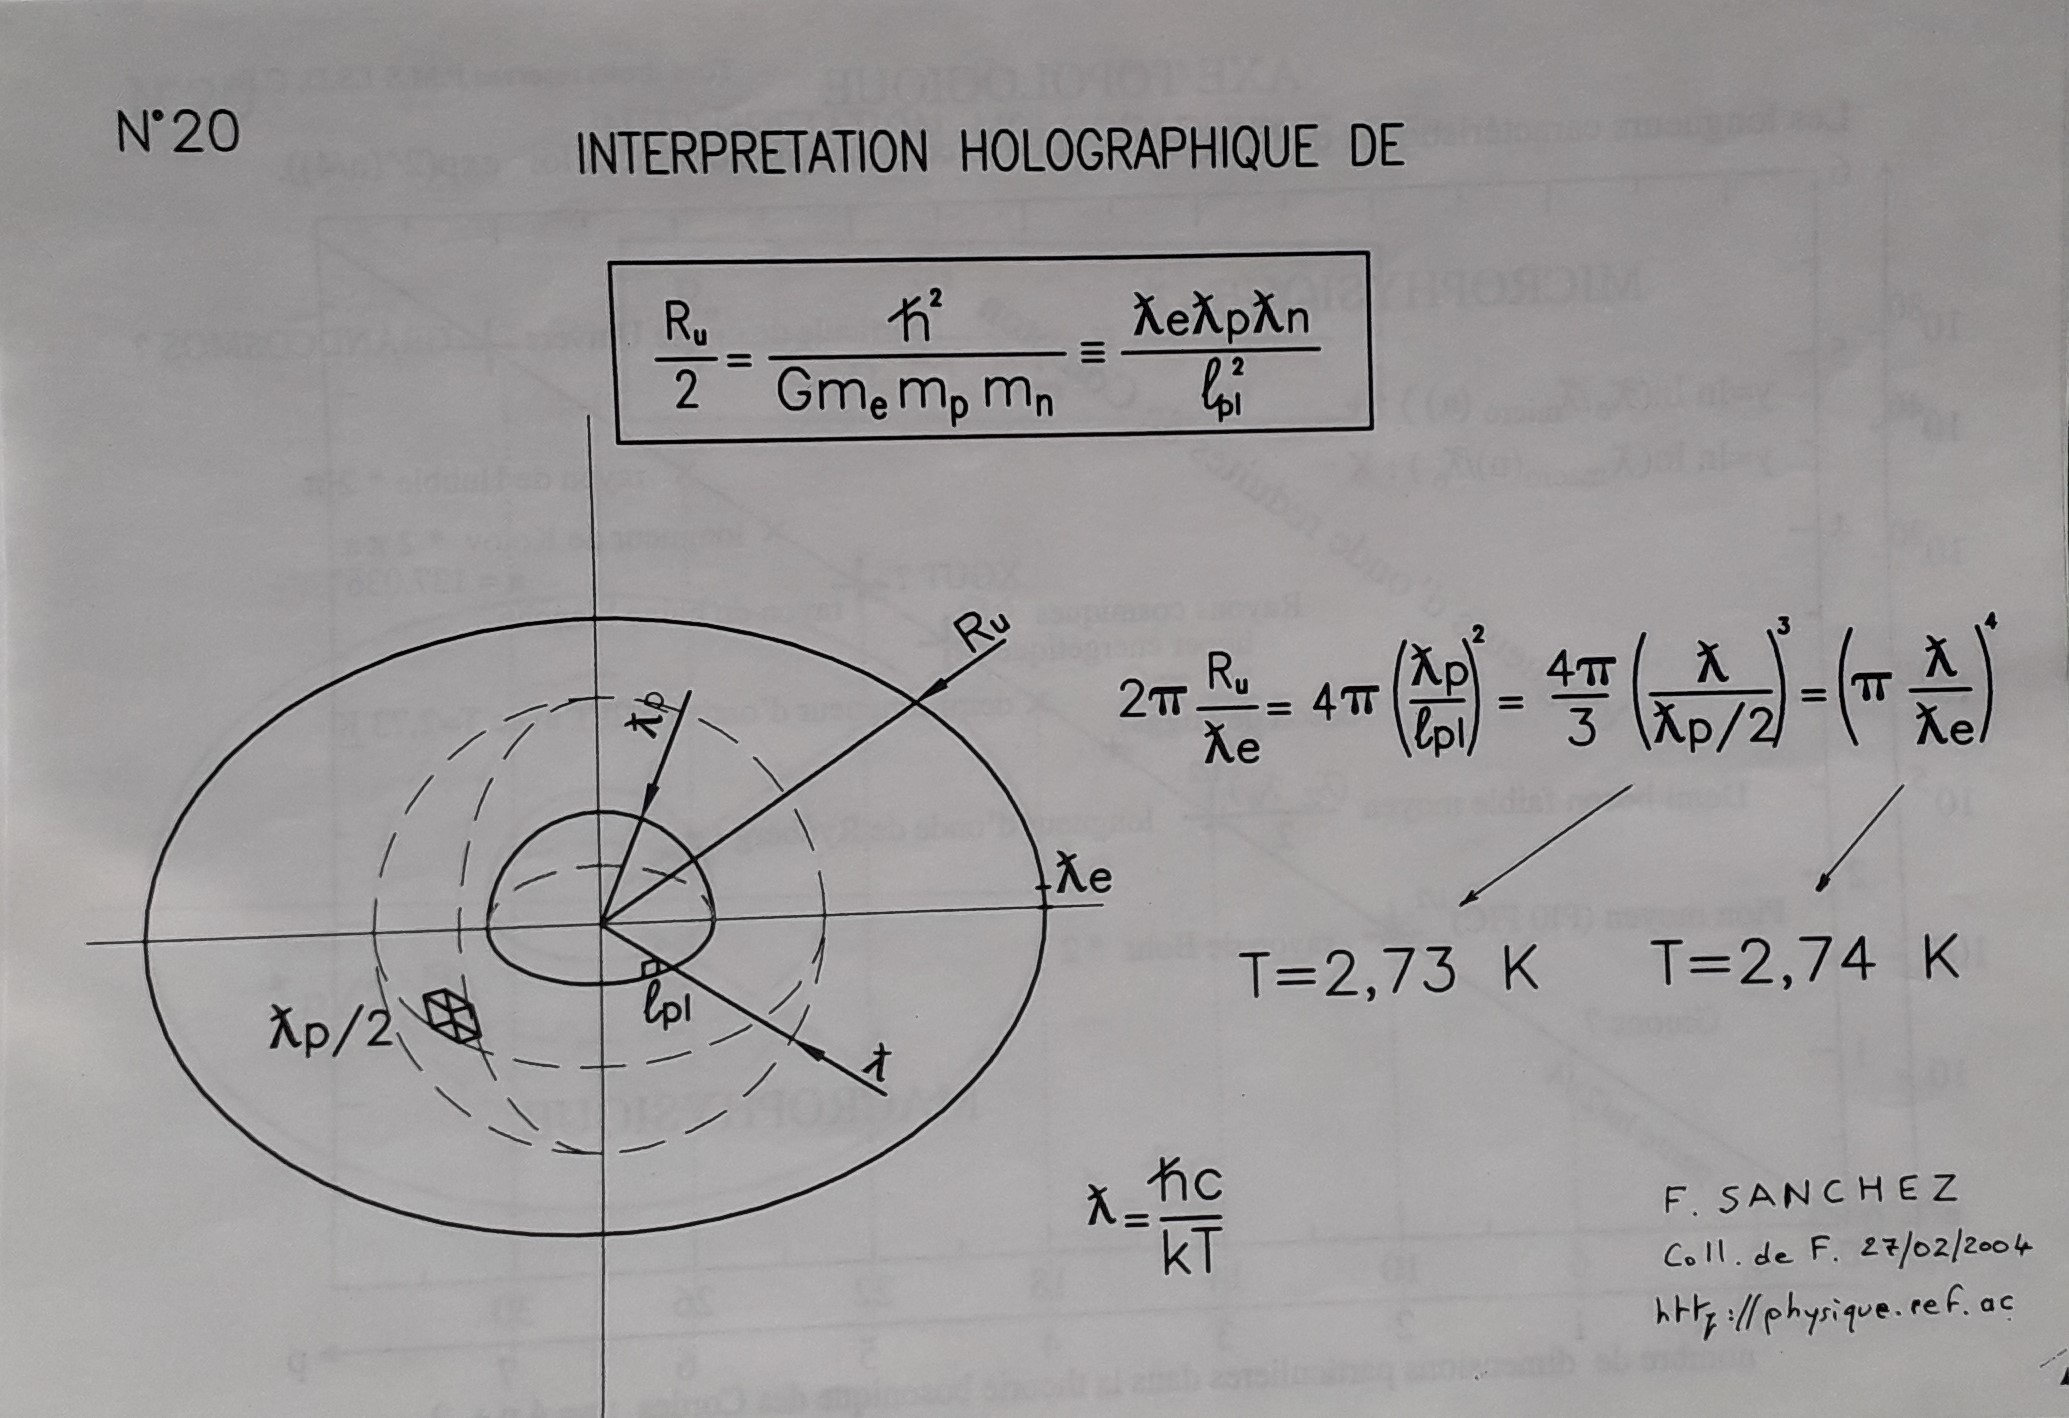
\includegraphics[width=12.5cm,height=7.5cm]{./figures/Holotemperature.jpg}
\caption[Interpretation holographique de la relation centrale. College de France]{\textit{Interprétation holographique de la relation centrale. Collège de France} Février 2004}
\label{fig:20:figure20}
\end{figure}

\begin{figure}
\centering
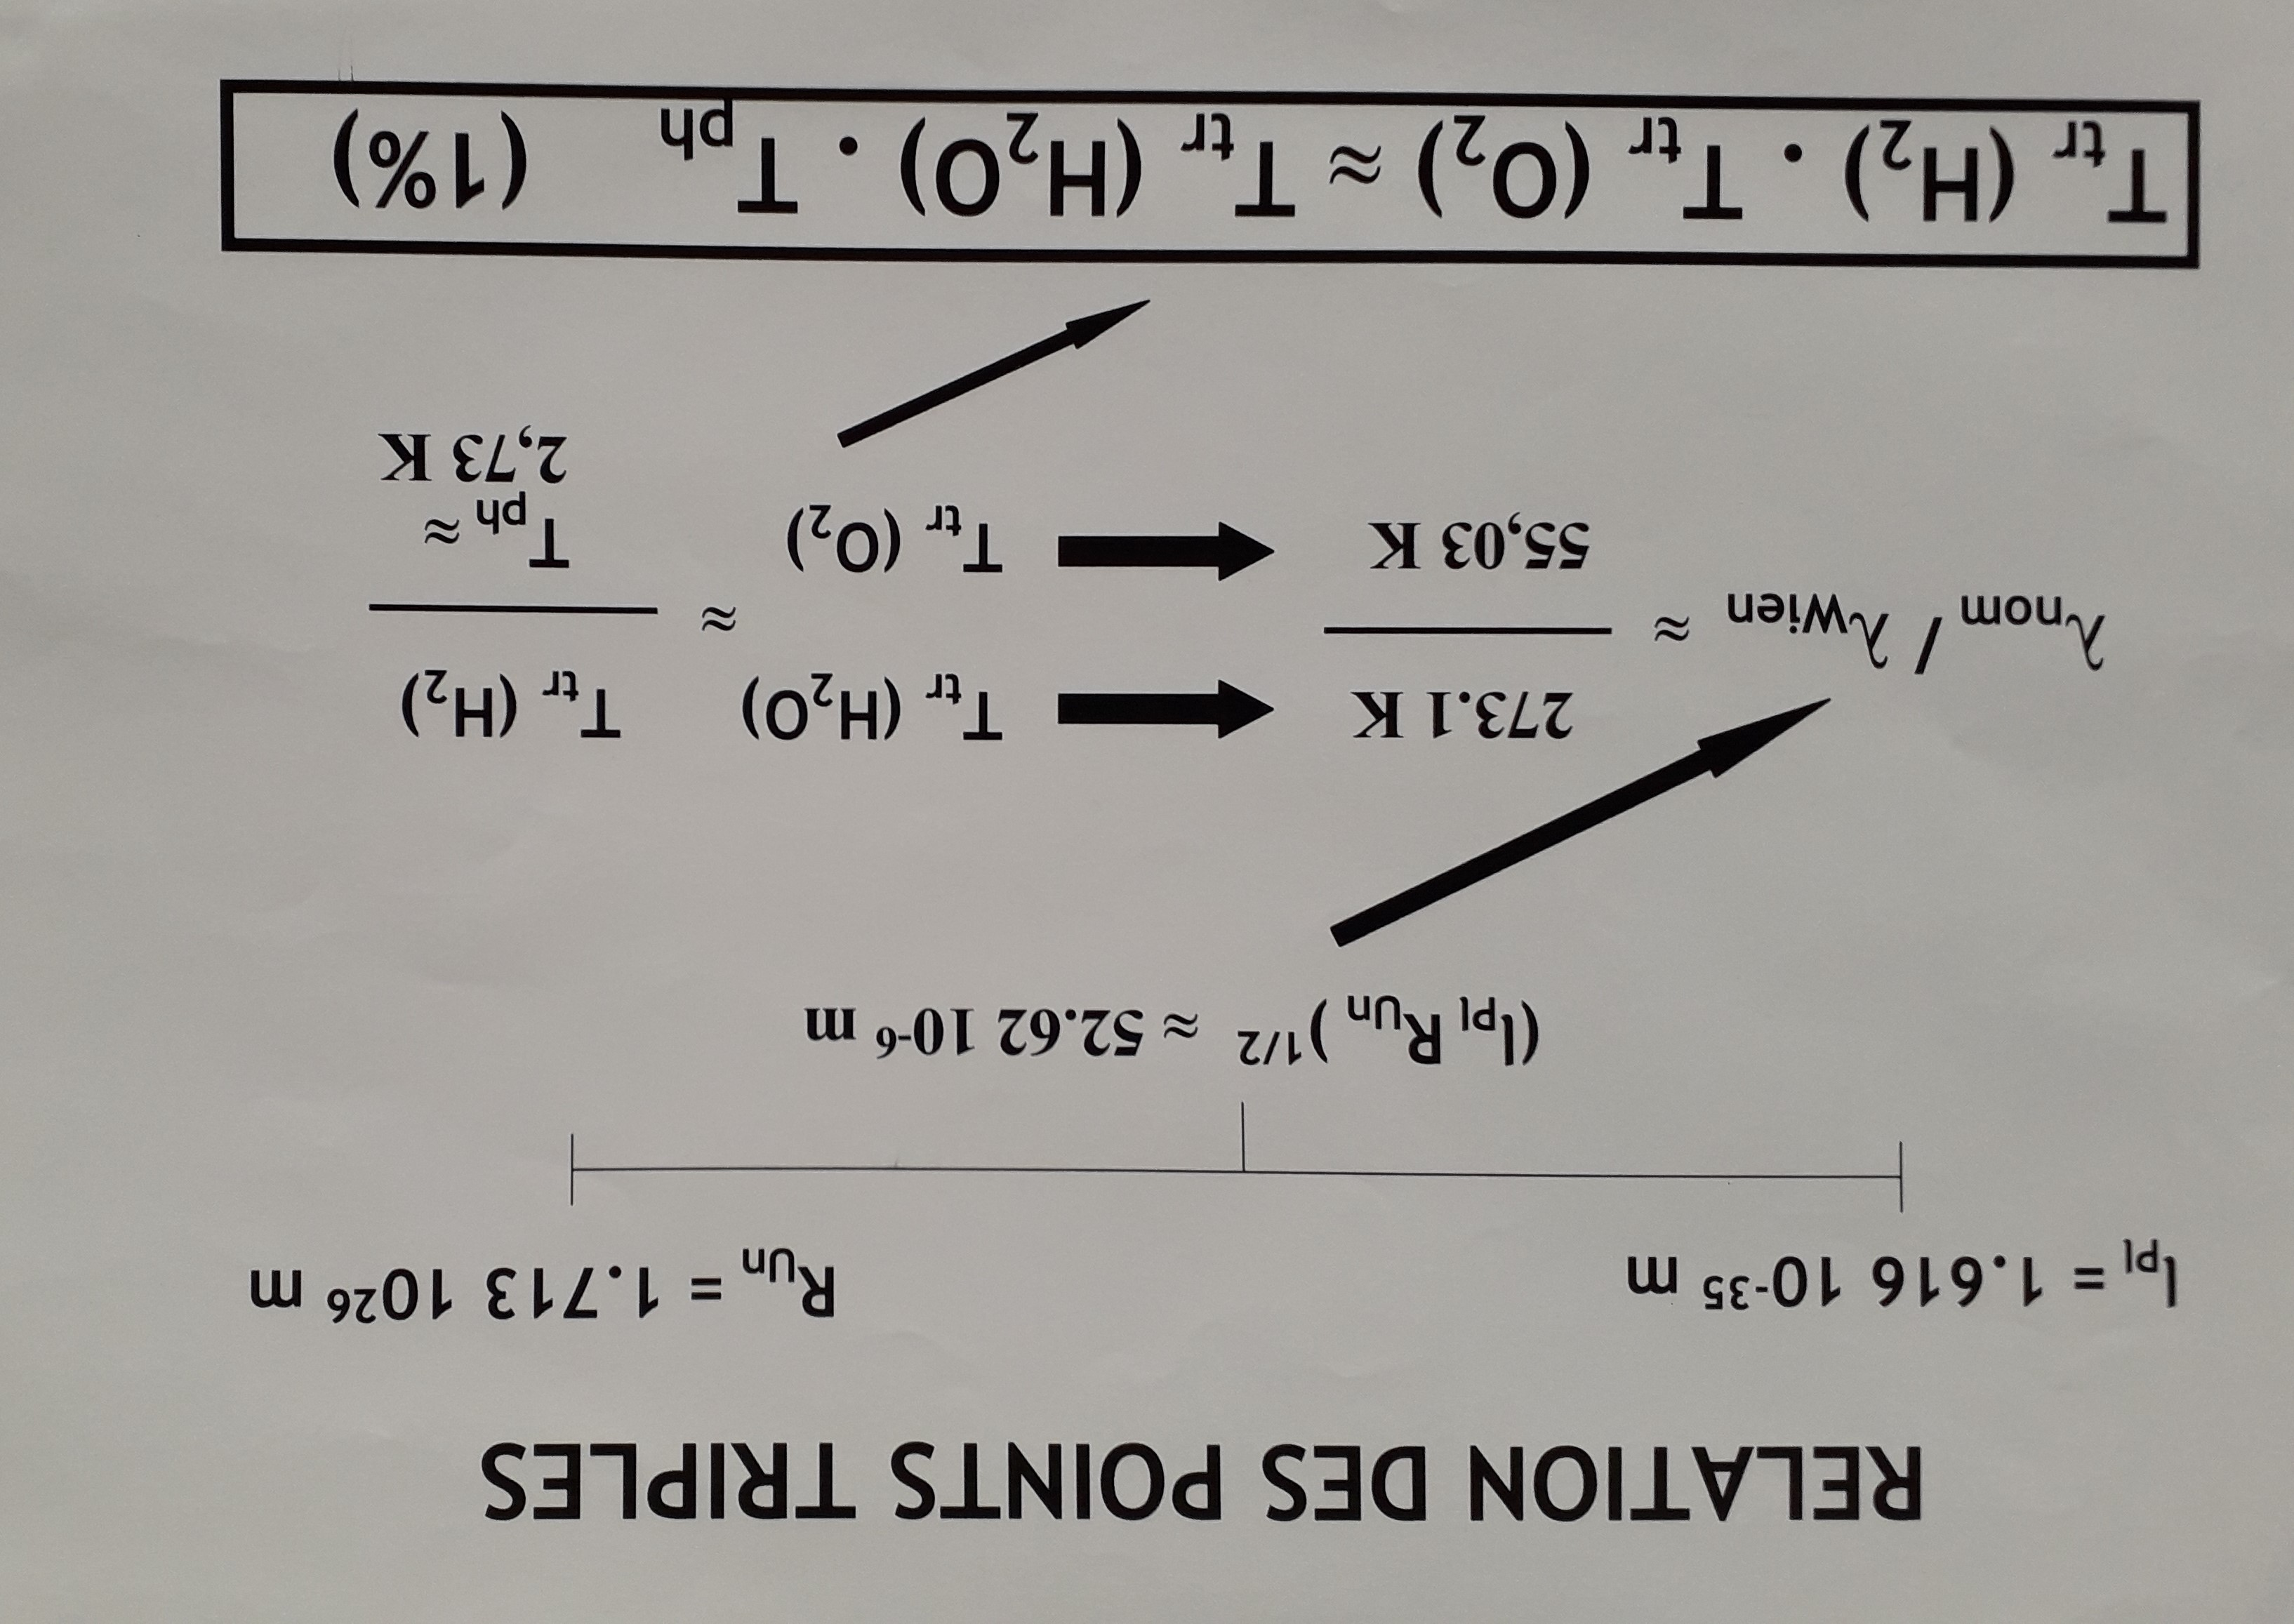
\includegraphics[width=12.5cm,height=7.5cm]{./figures/Zpointstriples.png}
\caption[Relation des Points Triples de l eau]{\textit{Relation des Points Triples de $H_2O$} - Collège de France 2004.} 
\label{fig:21:figure21}
\end{figure}

\clearpage

\begin{figure}
\centering
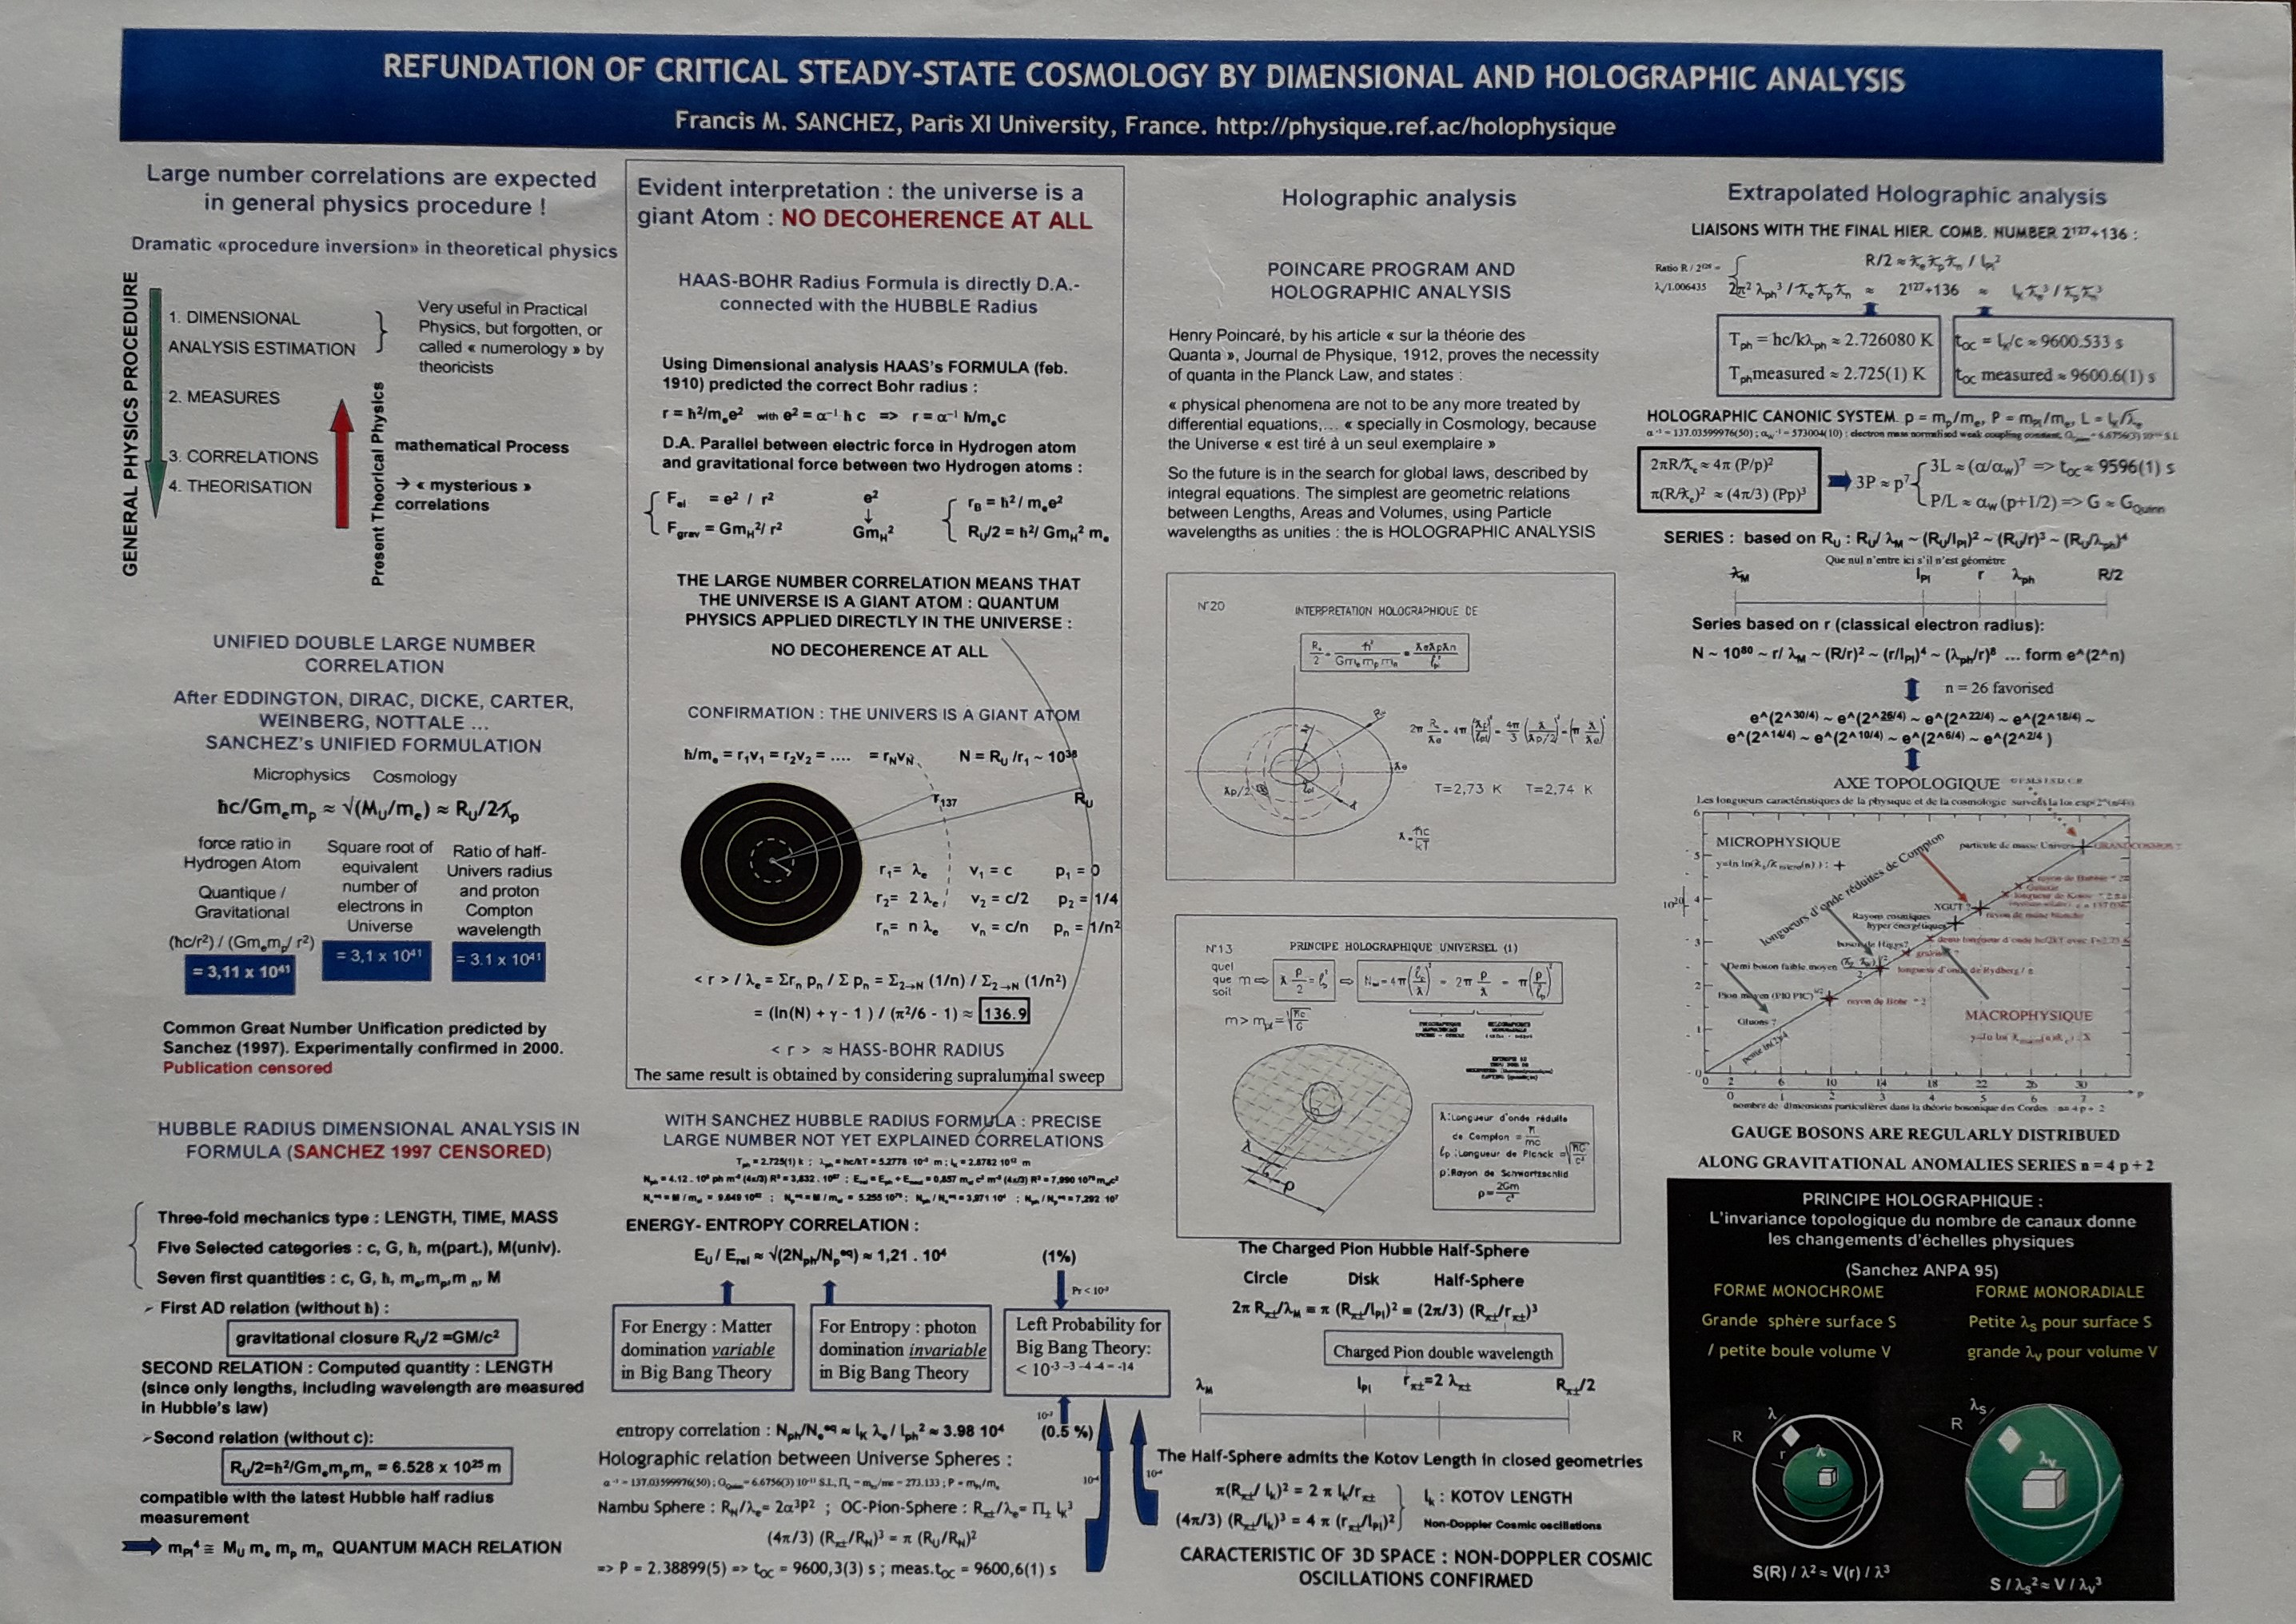
\includegraphics[width=12.5cm,height=7.5cm]{./figures/Collegedefrance2004.png}
\caption[Holophysique presentation College de France 2004]{\textit{Refundation of critical steady-state cosmology by Holographic and dimensional analysis} - Collège de France 2004.} 
\label{fig:22:figure22}
\end{figure}

\clearpage

\begin{figure}
\centering
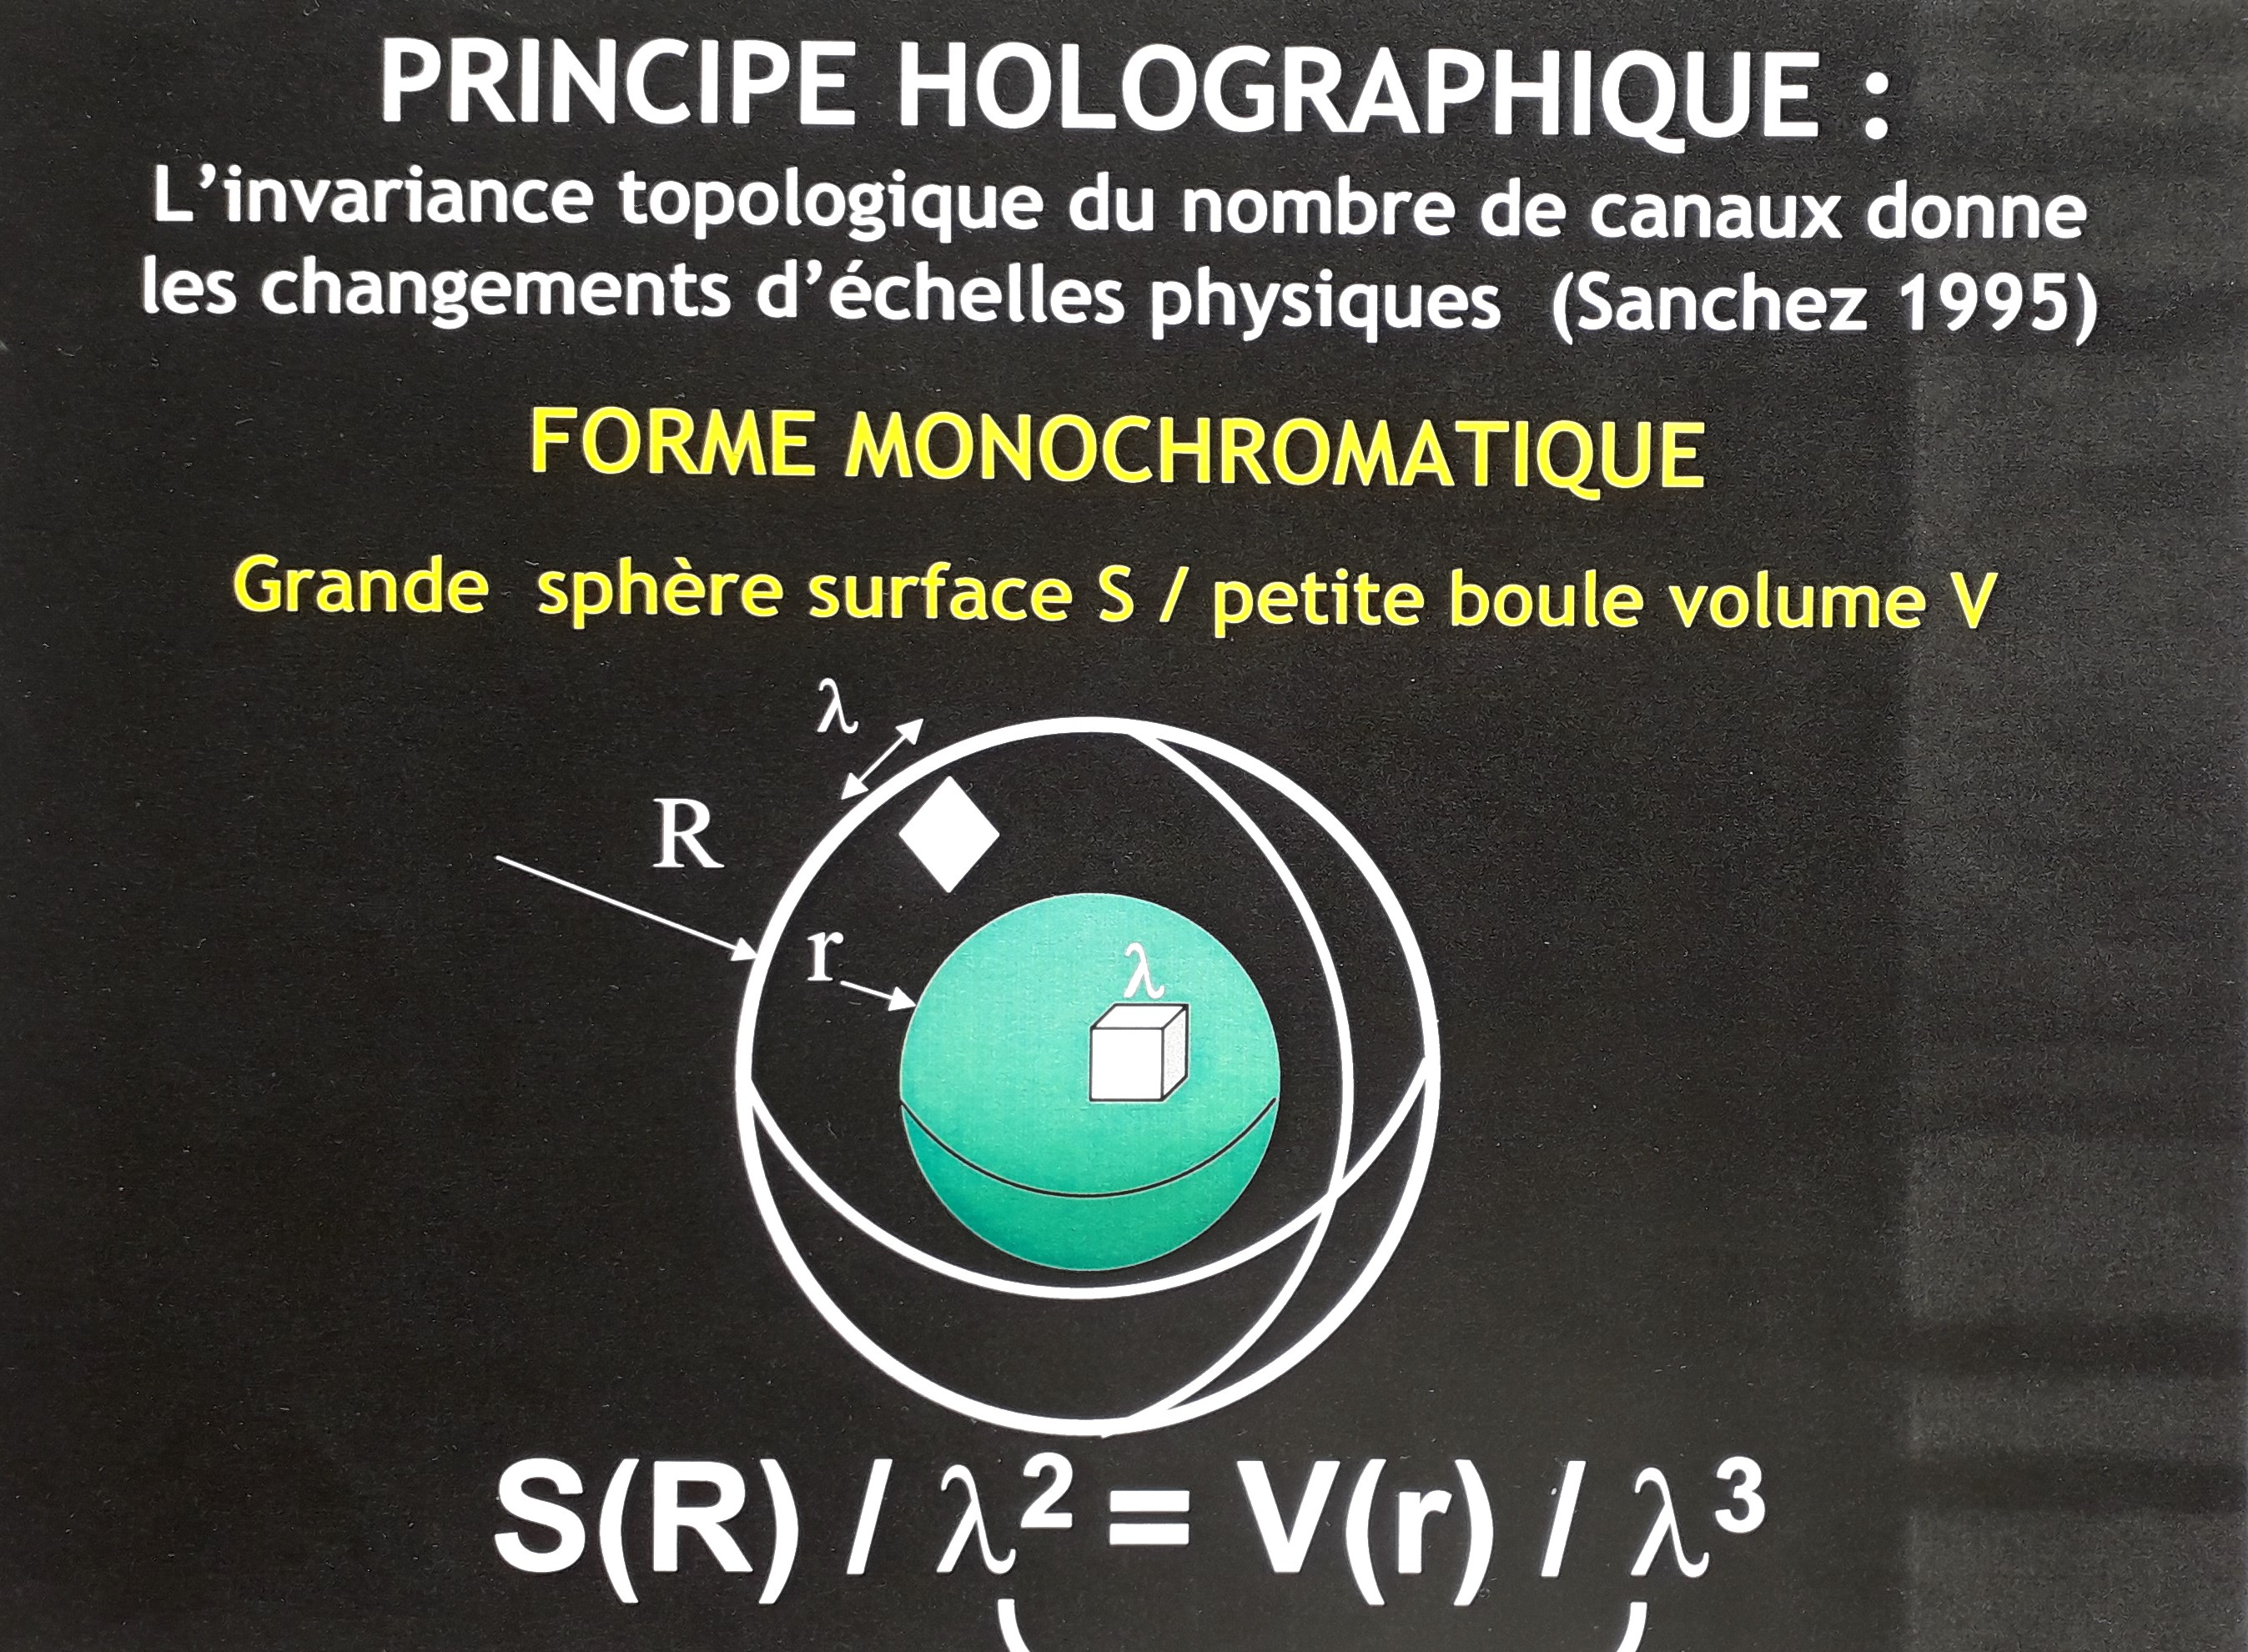
\includegraphics[width=12.5cm,height=7.5cm]{./figures/HPmonochro.jpg}
\caption[HP monochro Collège de France 2004]{\textit{HPmonochro, College de France} - date 2004.} 
\label{fig:23:figure23}
\end{figure}


\begin{figure}
\centering
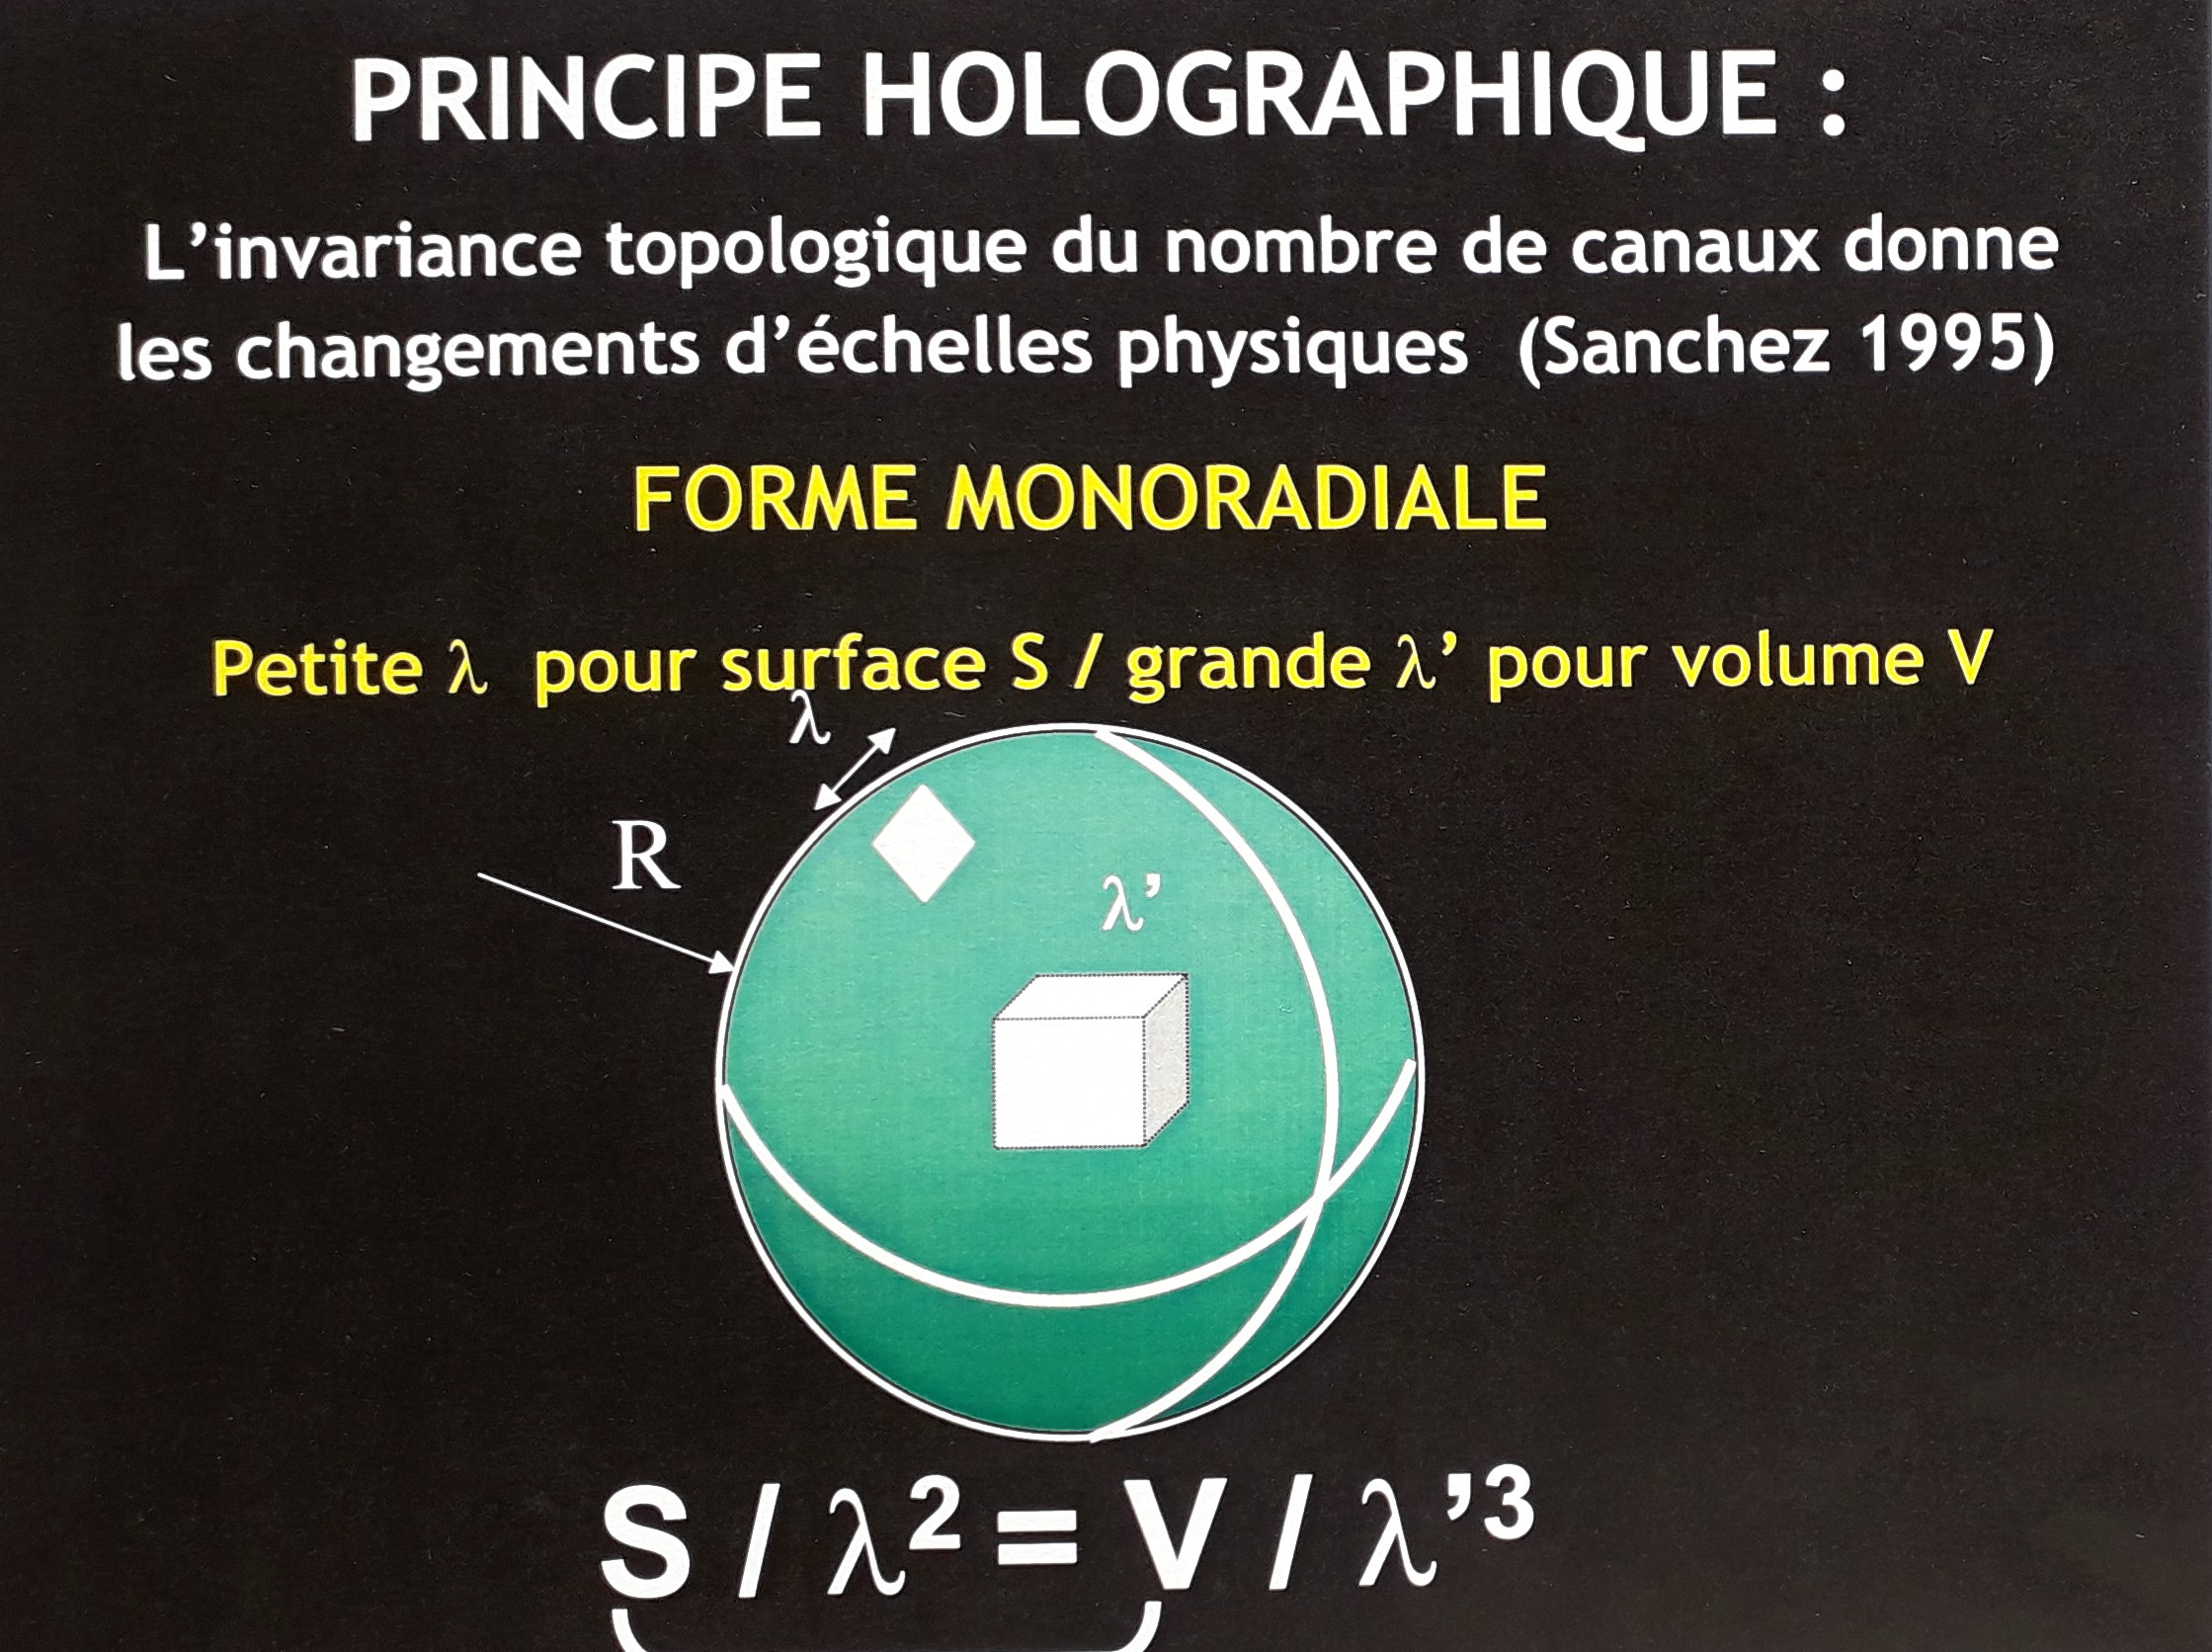
\includegraphics[width=12.5cm,height=7.5cm]{./figures/HPmonoradial.jpg}
\caption[HP monoradial Collège de France 2004]{\textit{HPmonoradial, College de France} - date 2004.} 
\label{fig:24:figure24}
\end{figure}

\clearpage

\begin{figure}
\centering
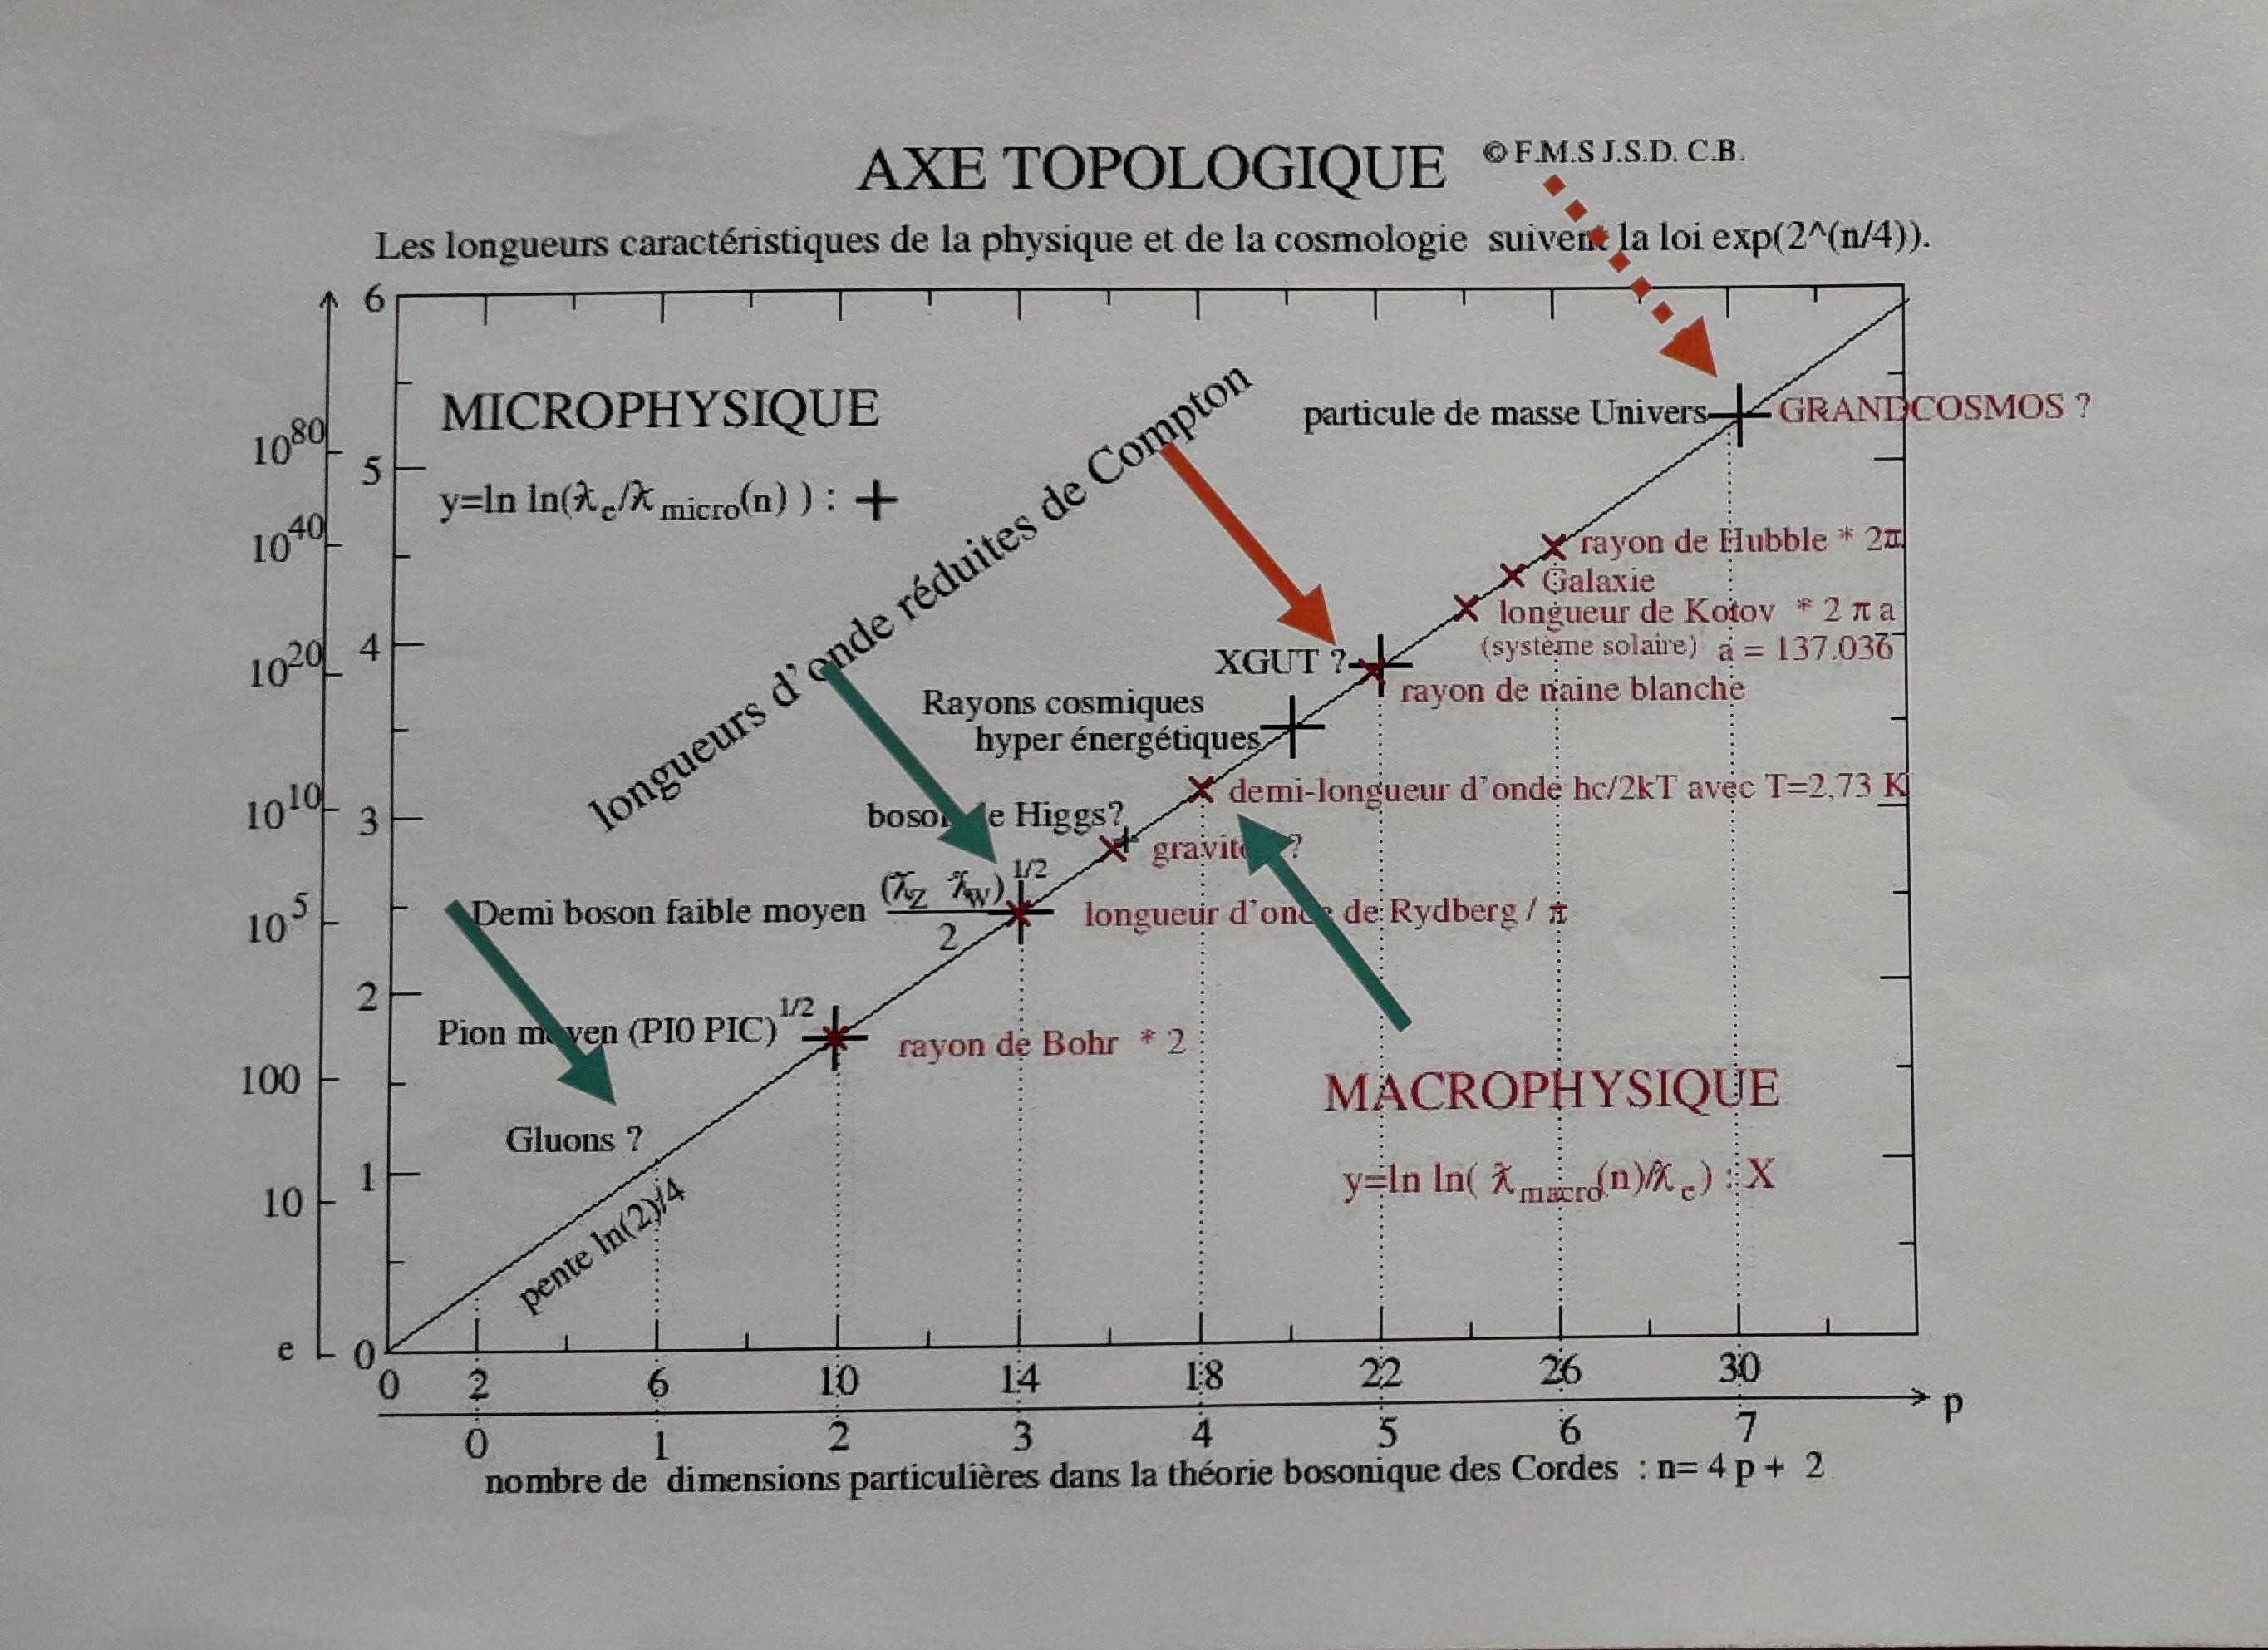
\includegraphics[width=12.5cm,height=7.5cm]{./figures/ATgaugebosons.jpg}
\caption[Axe Topologique: Bosons de jauge, Collège de France, 2004.]{\textit{Axe Topologique: Bosons de jauge, College de France} - date 2004.} 
\label{fig:25:figure25}
\end{figure}


\begin{figure}
\centering
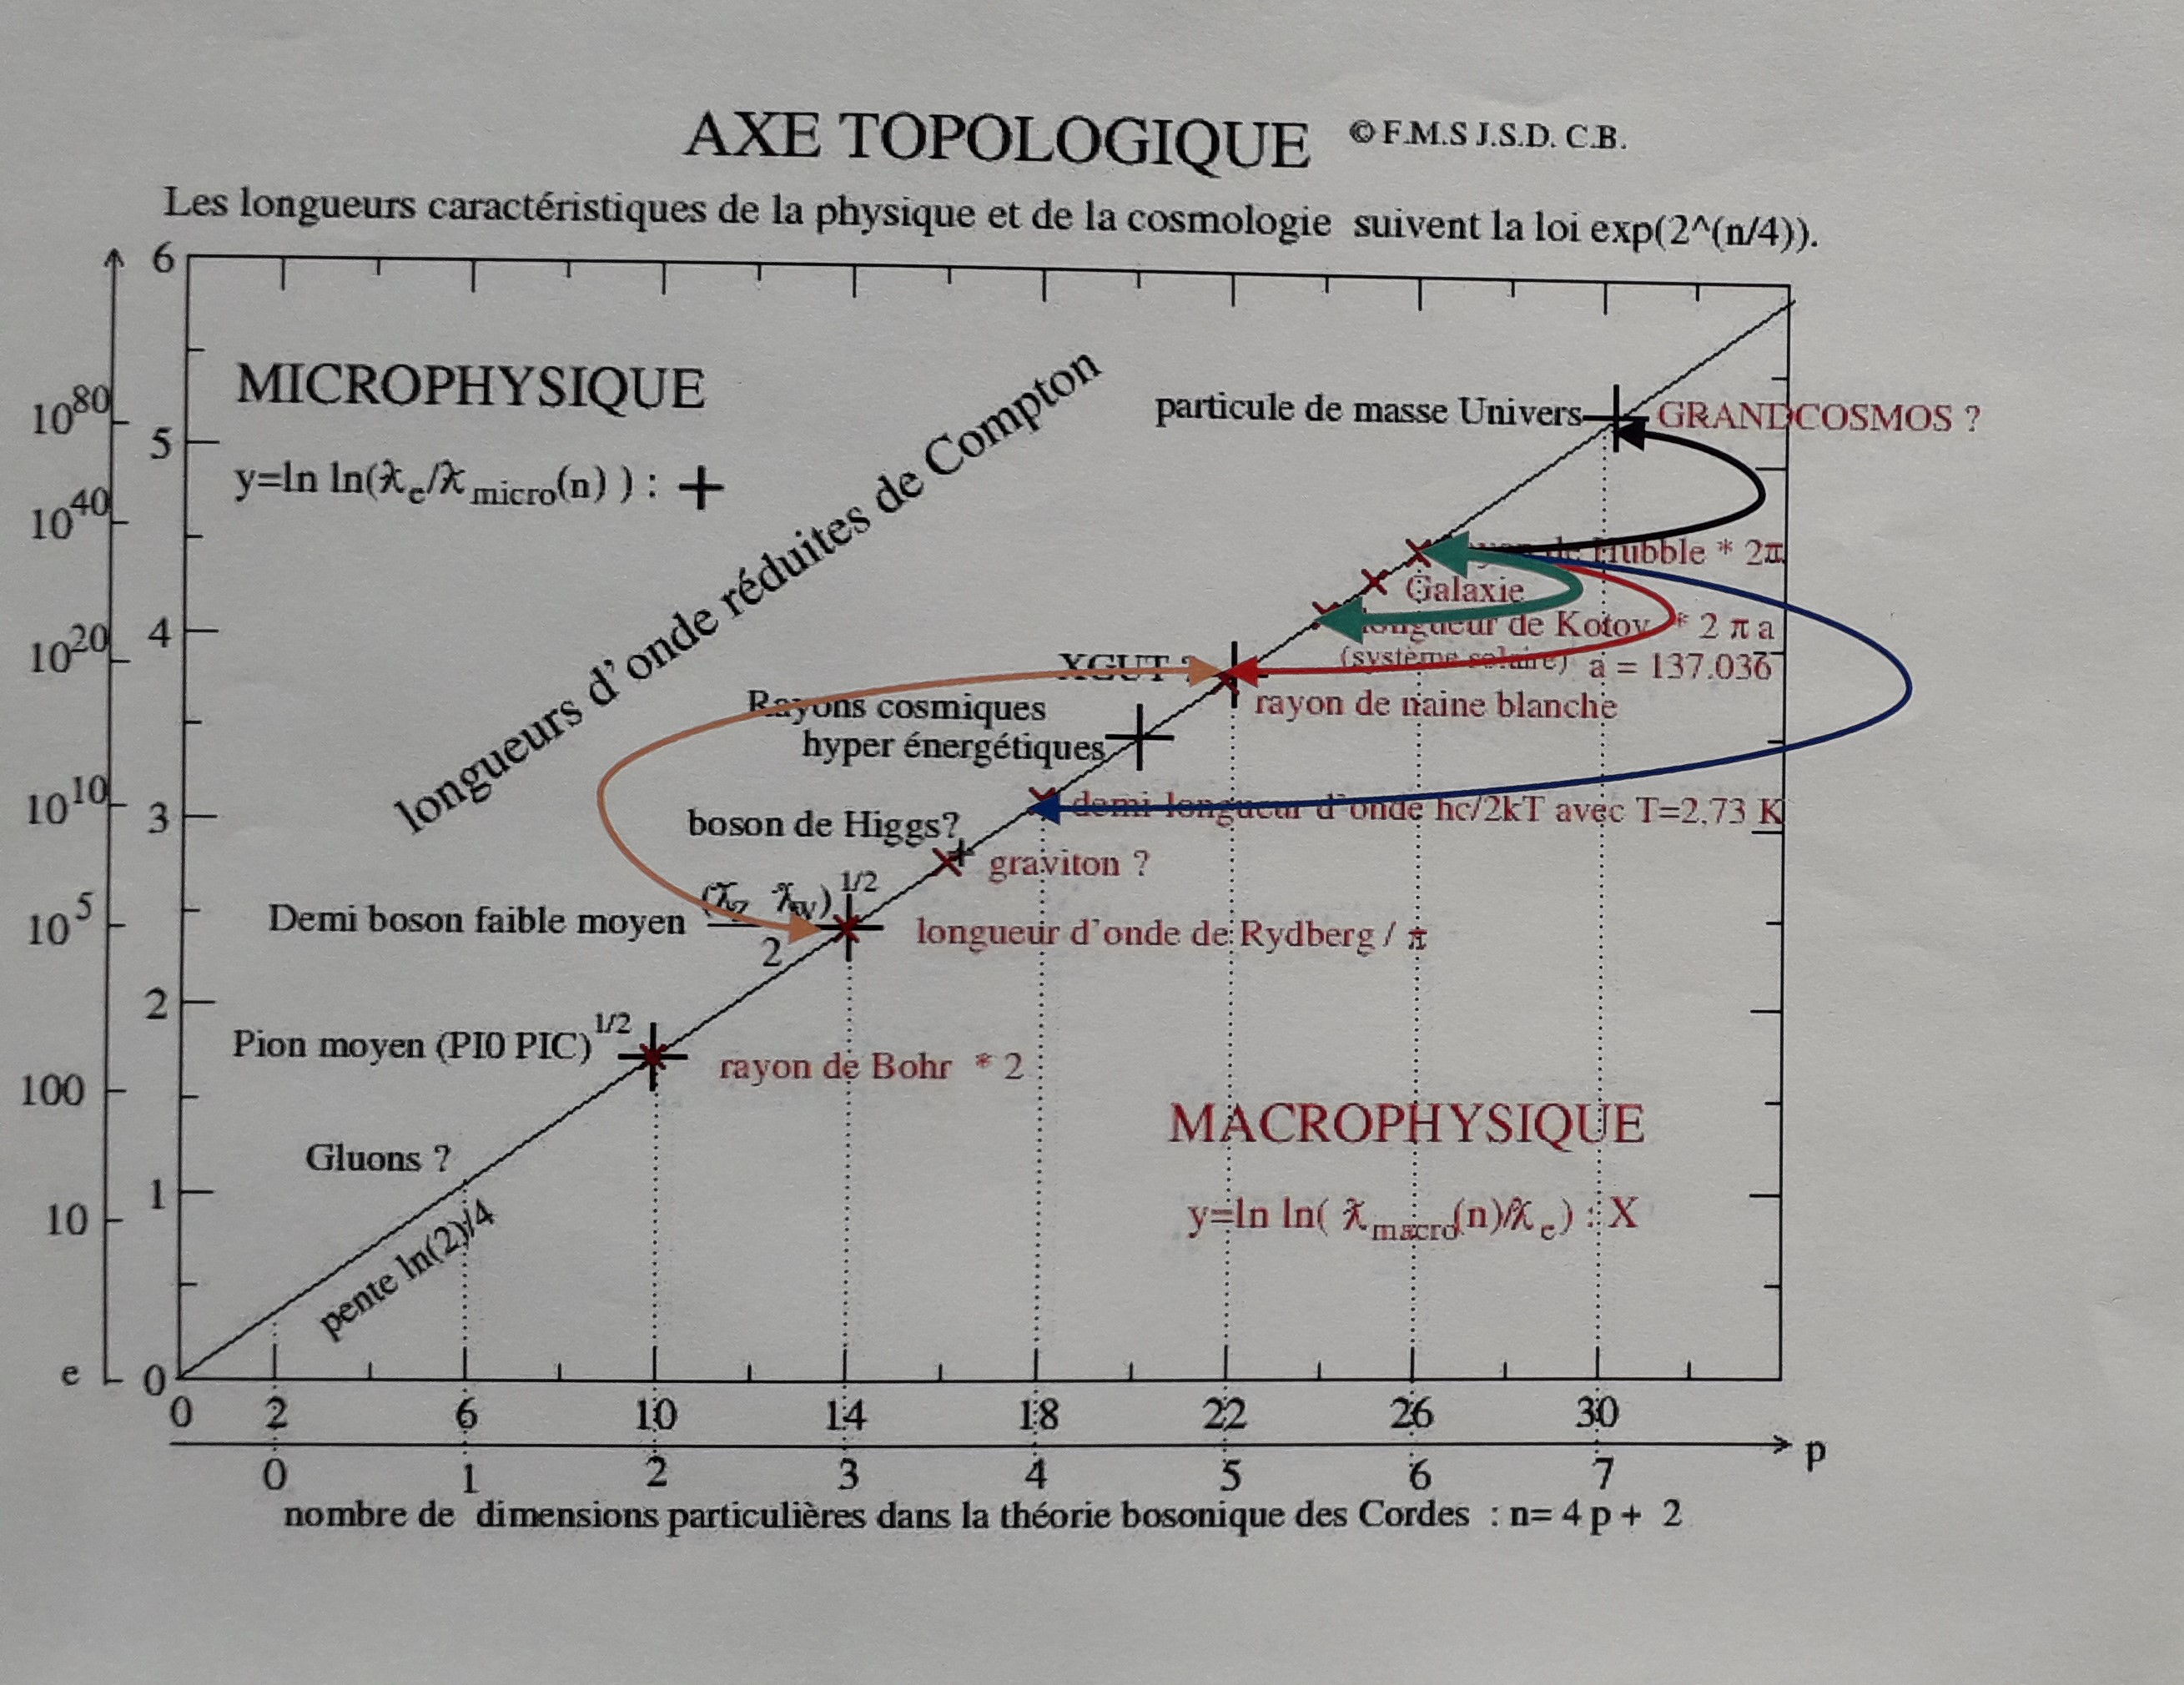
\includegraphics[width=12.5cm,height=7.5cm]{./figures/ATconexions.jpg}
\caption[Axe Topologique: Connexions, Collège de France, 2004.]{\textit{Axe Topologique: Connexions, College de France} - date 2004.} 
\label{fig:26:figure26}
\end{figure}

\clearpage

%\begin{figure}
%\centering
%%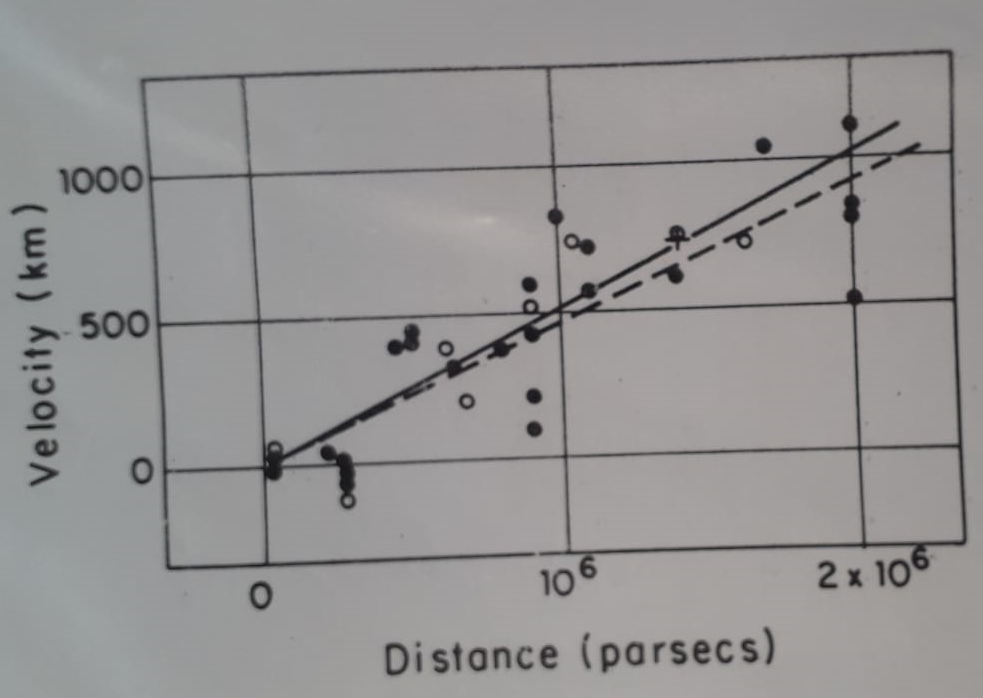
\includegraphics[width=14.5cm,height=8.6cm]{./figures/hubble-edwin-1929-ProcNaturalAcad.SciVol15p168.png}https://www.pnas.org/content/pnas/15/3/168/F2.large.jpg

%% \write18{wget https://www.pnas.org/content/pnas/15/3/168/F2.large.jpg}
%%\href{https://www.pnas.org/content/pnas/15/3/168/F2.large.jpg}{\incudegraphics{F2.large.jpg}}
%\includegraphics{hubble-orig.jpg}
%\caption [Edwin Hubble 1929]{\textit{Edwin Hubble ProcNaturalAcad-SciVol15p168} - Tracé .} 
%\label{fig:10:figure10}
%\end{figure}






\bibliographystyle{unsrt}  
%\bibliography{references}  %%% Remove comment to use the external .bib file (using bibtex).
%%% and comment out the ``thebibliography'' section.


%%% Comment out this section when you \bibliography{references} is enabled.
\begin{thebibliography}{1}

\bibitem{Sanchez3} Sanchez F.M. ``Towards the grand unified Holic Theory''. Current Issues in Cosmology. Ed. J.-C. Pecker and J. Narlikar. p. 257--260.
\newblock Cambridge Univ. Press, 2006

\bibitem{Sanchez4} Francis M. Sanchez ``Holic Principle: The coherence of the Universe`` (Sept 1995), 324--344.
\newblock Entelechies, 16th ANPA
\bibitem{Grosmann} Michel H. Grosmann and P. Meyrueis ``Optics and Photonics Applied to Communication and Processing''. SPIE.  Jan 1979.
%%\newblock Optics and Photonics Applied to Communication and Processing.
\newblock In {\em SPIE (SPIE), 1979 International Conference on}, pages . SPIE, 1979.
  
\bibitem{Grosmann2} Michel H. Grosmann, José Rebordão,  and Patrick Meyrueis, 1985,02,p761--765,Propagation Of Waves In Optical Systems: Reformulation Of Huyghens Principle For Aspheric Systems, volume 491, Proceedings of SPIE - The International Society for Optical Engineering, doi:10.1117/12.968010
\newblock In {\em Proceedings of SPIE - The International Society for Optical Engineering}. SPIE, 1985.
\bibitem{Kress} Digital Diffractive Optics: An Introduction to Planar Diffractive Optics and Related Technology, by B. Kress, P. Meyrueis, pp. 396. ISBN 0-471-98447-7. Wiley-VCH , October 2000.
\newblock An Introduction to Planar Diffractive Optics and Related Technology.
\bibitem{Sanchez5} F. M. Sanchez, V. Kotov, M. H. Grosmann, D. Weigel, R. Veysseyre, C. Bizouard, N. Flawisky, D. Gayral, L. Gueroult, ``Back to Cosmos''
\newblock {\em Progress in Physics}, 2019 (vol. 15), issue 2, http://www.ptep-online.com/2019/PP-57-12.PDF
\bibitem{Denisyuk} Yuri N. Denisyuk, ``Fundamentals of Holography'', p26--55
\newblock {\em State Optical S.I. Vavilov Institute}, 1978.
\bibitem{Tarasov} Lev V. Tarasov, ``Laser age in Optics'', p202
\newblock {\em Mir Publishers Moscow}, 1981.
\bibitem{Vienot} J-C Vienot, P. Smigielski, H. Royer ``Holographie Optique, Developpements-Applications'', preface de Dennis Gabor
\newblock {\em Dunod Ed.}, 1971.
\bibitem{Bjelkhagen} Hans I. Bjelkhagen, H. John Caulfield ``Selected Papers on Fundamental Techniques in Holography'', Holographic Cinematography: Principle of the holographic cinematography Victor G. Komar (in 1st European Congress on Optics Applied to Metrology, M. H. Grosmann, editor, 1977) p258, Vol. MS171
\newblock {\em SPIE Ed.}, 2001, https://spie.org/Publications/Book/436130
\bibitem{Gabor} Dennis gabor ``Nobel Lecture: Holography'', 1948–1971. Nobel Foundation.
\newblock {\em Nobel Media AB}, 2014.
\bibitem{French} A P French; G Delacote; J Souchon-Rouyer; Alfred Kastler; J B Yelnick; et al ``Einstein : le livre du centenaire''
\newblock {\em Hier et Demain}, 1979.
\bibitem{Koyre} A. KOYRÉ, ``Etudes d’Histoire de la pensée scientifique'', Paris, Gallimard, 1973, p. 54.
\newblock {\em Gallimard}, 1973.
\bibitem{Sherrard} Ph. SHERRARD, ``Human Image : World Image. The death and resurrection of sacred cosmology'', Limni, Evia, Grèce, Denise Harvey, 2004, (princeps par Golgonooza Press en 1992)
\newblock {\em Golgonooza Press}, 1992.
\bibitem{Galilee} GALILÉE, ``Il Saggiatore, in Le Opere di Galileo Galilei'', Ed ; Nazionale, A. Favaro, Florence, 21 vol., 1890-1909, vol. VI, p. 232.
\newblock {\em Ed Nazionale}, 1890-1909.
\bibitem{Beaty} William J. Beaty ``Drawing Holograms by Hand'' W. T. Plummer and L. R. Gardner, "A mechanically generated hologram", Applied Optics Vol.31, No. 31 (1 November 1992) pp.6585-6588
\newblock {\em http://holowiki.nss.rpi.edu/wiki/Scratch-O-Gram}, 1992.

\bibitem{ISL}  https://www.isl.eu
\newblock {\em https://www.isl.eu/documentation/rapports-annuels}, 1958.

\bibitem{Wu}  Junfei Wu et al. ``Progress in Precise Measurements of the Gravitational Constant''
\newblock {\em https://onlinelibrary.wiley.com/doi/full/10.1002/andp.201900013}, April 2019

\bibitem{Tanabashi} M. Tanabashi et al. ``The Review of Particle Physics''
\newblock {\em http://pdg.lbl.gov/2019/reviews/rpp2019-rev-history-plots.pdf}, 2019

\bibitem{Ives} Herbert IVES, Journal of the Optical Society of America Vol. 42, Issue 8, pp. 540-543 
\newblock {\em https://doi.org/10.1364/JOSA.42.000540}, 1952

\bibitem{Lecompte} F. Sanchez C. Lecompte ``Q-Switched $Nd^3+$ Glass Laser of Variable Temporal Coherence'', Applied optics, vol.13, 05.1974, p1071--1076
\newblock {\em https://doi.org/10.1364/AO.13.001071}

\bibitem{Mainfray} C. Lecompte, G. Mainfray, C. Manus, F. Sanchez ``Laser temporal-coherence effects on multiphoton ionization processes'', Physical Review A 11(3), vol.11, 03.1975
\newblock {\em https://journals.aps.org/pra/abstract/10.1103/PhysRevA.11.1009}

\bibitem{Gabrielse} G. Gabrielse et al,, ``New Determination of the Fine Structure Constant from the Electron g Value and  QED'',  Phys. Rev. Lett. 97, 030802 (2006)
\newblock {\em http://hussle.harvard.edu/~gabrielse/gabrielse/papers/2006/NewFineStructureConstant.pdf}, 2006

\bibitem{Merkatas} C. Merkatas et. al., ``Consensus Value for the Newtonian Constant of Gravitation'' Xiv:1905.09551v1 [physics.data-an] 23 May 2019
\newblock {\em https://arxiv.org/abs/1905.09551v1}, 2019

\bibitem{Grosmann3} Grosmann, Michel and Rebordão, José and Meyrueis, Patrick., ``Propagation Of Waves In Optical Systems: Reformulation Of Huyghens Principle For Aspheric'' Proceedings of SPIE - The International Society for Optical Engineering,vol.491, 02.1985, p761--765
\newblock {\em https://www.spiedigitallibrary.org/conference-proceedings-of-spie/0491/1/Propagation-Of-Waves-In-Optical-Systems--Reformulation-Of-Huyghens/10.1117/12.968010.short?SSO=1}, 1985

\bibitem{Gentet} Yves Gentet, Philippe Gentet: Ultimate emulsion and its applications: A laboratory-made silver halide emulsion of optimized quality for monochromatic pulsed and full color holography.
\newblock {\em https://www.spiedigitallibrary.org/conference-proceedings-of-spie/4149/1/Ultimate-emulsion-and-its-applications--a-laboratory-made-silver/10.1117/12.402459.short?SSO=1}, OCT 2000

\end{thebibliography}
\end{appendix}

\end{document}
